% Copyright 2026 MiniLangProject contributors
% SPDX-License-Identifier: Apache-2.0
\documentclass[11pt,a4paper,oneside,openany]{book}
% Source baseline. Change this only after reviewing the corresponding revision.
\newcommand{\SourceCommit}{ce5b0ad6884b5d053dc455474e500117bb73b19a}
\newcommand{\SourceShort}{ce5b0ad}
\newcommand{\EditionDate}{25 November 2026}
\newcommand{\ManualVersion}{1.1}
\newcommand{\RepositoryURL}{https://github.com/MiniLangProject/MiniSQL}

\usepackage[T1]{fontenc}
\usepackage[utf8]{inputenc}
\usepackage{lmodern}
\ifdefined\pdfmapfile\pdfmapfile{+lm.map}\fi
\usepackage{microtype}
\usepackage[a4paper,inner=24mm,outer=23mm,top=24mm,bottom=25mm,headheight=15pt,headsep=8mm]{geometry}
\usepackage{graphicx,xcolor,booktabs,longtable,array,tabularx,multirow}
\usepackage{amsmath,amssymb}
\usepackage{enumitem}
\usepackage{listings,upquote}
\usepackage{tikz}
\usetikzlibrary{arrows.meta,positioning,calc,fit,backgrounds,shapes.geometric}
\usepackage[most]{tcolorbox}
\usepackage{titlesec,fancyhdr,needspace}
\usepackage{makeidx}
\usepackage{hyperref}
\usepackage{bookmark}
\usepackage{url}
\definecolor{Navy}{HTML}{142B45}
\definecolor{Teal}{HTML}{087F8C}
\definecolor{Ink}{HTML}{213547}
\definecolor{Muted}{HTML}{56687A}
\definecolor{Pale}{HTML}{EFF5F8}
\definecolor{CodeBg}{HTML}{F4F7FA}
\definecolor{Rule}{HTML}{CCD8E3}
\definecolor{Amber}{HTML}{A85E06}
\definecolor{AmberBg}{HTML}{FFF5E5}
\hypersetup{colorlinks=true,linkcolor=Teal,urlcolor=Teal,citecolor=Teal,
  pdftitle={MiniSQL User Manual},pdfauthor={MiniLangProject},
  pdfsubject={Implementation-based English user manual; storage format 2},
  pdfkeywords={MiniSQL, SQL, administration, MiniLang, storage format 2},
  bookmarksnumbered=true,bookmarksopen=true,bookmarksopenlevel=1}
\urlstyle{tt}
\setlength{\emergencystretch}{3em}
\setlength{\parskip}{.35em}
\setlength{\parindent}{0pt}
\setlength{\tabcolsep}{5pt}
\renewcommand{\arraystretch}{1.16}
\setcounter{secnumdepth}{2}
\setcounter{tocdepth}{1}
\setlist{nosep,topsep=4pt,itemsep=3pt,leftmargin=1.6em}
\titleformat{\chapter}[display]{\sffamily\bfseries\color{Navy}\raggedright\hyphenpenalty=10000\exhyphenpenalty=10000}{\color{Teal}\large \MakeUppercase{\chaptertitlename} \thechapter}{8pt}{\Huge}
\titlespacing*{\chapter}{0pt}{-8pt}{25pt}
\titleformat{\section}{\Large\sffamily\bfseries\color{Navy}}{\thesection}{.7em}{}
\titleformat{\subsection}{\large\sffamily\bfseries\color{Teal}}{\thesubsection}{.7em}{}
\titleformat{\subsubsection}{\normalsize\sffamily\bfseries\color{Navy}}{}{0pt}{}
\titlespacing*{\section}{0pt}{20pt}{7pt}
\titlespacing*{\subsection}{0pt}{14pt}{5pt}
\pagestyle{fancy}
\fancyhf{}
\fancyhead[L]{\sffamily\small\color{Navy}\textbf{MiniSQL}\enspace /\enspace User Manual}
\fancyhead[R]{\sffamily\footnotesize\color{Muted}Storage format 2}
\fancyfoot[L]{\sffamily\footnotesize\color{Muted}Implementation edition\enspace\SourceShort}
\fancyfoot[R]{\sffamily\color{Navy}\thepage}
\renewcommand{\headrulewidth}{.4pt}
\renewcommand{\footrulewidth}{0pt}
\fancypagestyle{plain}{\fancyhf{}\fancyfoot[L]{\sffamily\footnotesize\color{Muted}MiniSQL / User Manual}\fancyfoot[R]{\sffamily\color{Navy}\thepage}\renewcommand{\headrulewidth}{0pt}}
\newcommand{\code}[1]{\texttt{#1}}
\newcommand{\tip}[2]{\begin{tcolorbox}[enhanced,colback=Pale,colframe=Teal,boxrule=.4pt,leftrule=2.5pt,arc=1mm,title={#1},fonttitle=\sffamily\bfseries,coltitle=Navy,colbacktitle=Pale,attach title to upper={\par\smallskip},before skip=9pt,after skip=9pt]#2\end{tcolorbox}}
\newcommand{\warning}[2]{\begin{tcolorbox}[enhanced,colback=AmberBg,colframe=Amber,boxrule=.4pt,leftrule=2.5pt,arc=1mm,title={#1},fonttitle=\sffamily\bfseries,coltitle=Amber,colbacktitle=AmberBg,attach title to upper={\par\smallskip},before skip=9pt,after skip=9pt]#2\end{tcolorbox}}
\newcommand{\sourcecode}[2]{\par\smallskip{\footnotesize\color{Muted}\textbf{Implementation evidence:} \href{\RepositoryURL/blob/\SourceCommit/#1}{\nolinkurl{#1}}. #2\par}\smallskip}
\newcommand{\learning}[1]{\tip{What you will learn}{#1}}
\lstdefinestyle{manual}{basicstyle=\ttfamily\footnotesize,keywordstyle=\color{Teal}\bfseries,commentstyle=\color{Muted}\itshape,stringstyle=\color{Amber},backgroundcolor=\color{CodeBg},rulecolor=\color{Rule},frame=single,framerule=.4pt,framesep=7pt,xleftmargin=8pt,xrightmargin=8pt,breaklines=true,breakatwhitespace=false,columns=fullflexible,keepspaces=true,showstringspaces=false,tabsize=2,aboveskip=11pt,belowskip=9pt,upquote=true,captionpos=b}
\lstset{style=manual}
\lstdefinelanguage{json}{morestring=[b]",morekeywords={true,false,null},sensitive=true}
\lstdefinelanguage{PowerShell}{morekeywords={param,if,else,foreach,in,try,catch,finally,throw,function,return},morecomment=[l]{\#},morestring=[b]",morestring=[b]'}
\tikzset{box/.style={draw=Rule,fill=Pale,rounded corners=2pt,align=center,font=\sffamily\small,inner sep=7pt},strong/.style={box,draw=Teal,fill=Teal!9},arrow/.style={-{Stealth[length=2.5mm]},thick,draw=Teal},smalllabel/.style={font=\sffamily\scriptsize,color=Muted,align=center}}
\makeindex

% Keep short executable examples from starting at the bottom of a page.
\BeforeBeginEnvironment{lstlisting}{\Needspace{8\baselineskip}}

\begin{document}
\begin{titlepage}

\begin{tikzpicture}[remember picture,overlay]
\fill[Navy] (current page.south west) rectangle (current page.north east);
\fill[Teal] ([xshift=19mm]current page.south west) rectangle ([xshift=23mm]current page.north west);
\foreach \r in {0,1,2,3,4}{\foreach \c in {0,1,2}{\fill[white,opacity=.07] ([xshift=133mm+\c*13mm,yshift=-39mm-\r*13mm]current page.north west) rectangle ++(10mm,-10mm);}}
\node[anchor=north west,text=white,align=left,text width=155mm] at ([xshift=34mm,yshift=-38mm]current page.north west) {\sffamily\large\bfseries MINILANG PROJECT};
\node[anchor=north west,text=white,align=left,text width=155mm] at ([xshift=34mm,yshift=-81mm]current page.north west) {\sffamily\fontsize{52}{58}\selectfont\bfseries MiniSQL\\[8mm]\fontsize{30}{36}\selectfont User Manual};
\node[anchor=north west,text=white,align=left,text width=141mm] at ([xshift=34mm,yshift=-153mm]current page.north west) {\sffamily\Large From your first database\\to SQL, operations and internals\\[10mm]\normalsize A practical course and implementation reference\\with worked examples, diagrams and exercises};
\node[anchor=south west,text=white,align=left,text width=146mm] at ([xshift=34mm,yshift=28mm]current page.south west) {\sffamily\small\textbf{IMPLEMENTATION EDITION}\quad\EditionDate\\[3mm]Source revision \SourceShort\quad |\quad Storage format 2\quad |\quad Wire protocol 1};
\end{tikzpicture}
\end{titlepage}
\frontmatter
\chapter*{About this edition}
\addcontentsline{toc}{chapter}{About this edition}
This book teaches MiniSQL as it is implemented in the repository at revision
\href{\RepositoryURL/commit/\SourceCommit}{\texttt{\SourceShort}}.
It combines a course for a first-time database user with a reference for the
person who develops applications, operates a server, diagnoses a slow query,
or needs to understand a database file. All prose, examples and figure sources
are included beside this PDF so the book can evolve with the engine.

\begin{table}[htbp]\centering
\caption{The identity of the implementation described in this book}
\begin{tabularx}{\linewidth}{p{.29\linewidth}X}
\toprule
Item & This edition\\\midrule
Repository & \url{https://github.com/MiniLangProject/MiniSQL}\\
Source baseline & \texttt{\SourceShort}; full identifier in \path{edition.tex}\\
Application version banner & MiniSQL 1.1.1\\
Storage generation & 2, an unreleased development change at this revision\\
Wire protocol & 1; independent of storage generation\\
Main operating targets & Native Windows x64 and Linux x64\\
Graphical Workbench & Native Windows application\\
Manual edition & \ManualVersion, \EditionDate\\\bottomrule
\end{tabularx}
\end{table}

\warning{Read the version identity before opening existing data}{The
\code{1.1.1} program banner does not mean that the current development tree
opens a released format-1 database. Storage format 2 rejects format-1 files.
There is no automatic format-1 converter. Changing a version number in a file
or configuration does not migrate its contents. Keep the old executable and
its database together while preparing a separately verified logical rebuild.}

\section*{How the book establishes a claim}
The primary sources are the program entry points, parser, binder, executor,
storage code, connector implementations and tests at the pinned revision.
An \emph{Implementation evidence} note identifies the relevant repository
file, with a link fixed to the source commit. Existing release guides and
historical acceptance reports provide context; they do not override behavior
in the current code. The executable teaching examples and focused edge-case
probes are recorded in \path{validation.json}. The appendix states precisely
what was executed and what was reviewed from source.

This matters because a parser can recognize a clause that the executor later
rejects. It also matters because implementing a storage type does not prove
that all arithmetic, comparison and wire-conversion paths have standard SQL
semantics. The book marks such cases at the point where a learner would
otherwise be likely to rely on them.

\section*{Learning routes}
Read Chapters 1--3 in order if you have never used a relational database.
Continue through the language chapters while running the supplied SQL files.
Use the workshops to check understanding. The operations chapters then turn a
local experiment into a managed service: accounts, limits, backups, restore
verification and replication. Application developers should also read the
connector chapter before adopting transaction or type-conversion assumptions
from another database driver. The performance and storage chapters explain
how to investigate behavior rather than guess.

An experienced SQL user can start with the type and language differences,
the transactions chapter and the compatibility matrix, then use the detailed
reference. An operator can start with installation and the server-mode table,
but should still read the version warning and the limitations below.

\section*{Conventions}
SQL keywords are capitalized for readability, not as a requirement. Examples
use lowercase, uncomplicated identifiers. Angle-bracketed text in command
syntax, such as \code{<database-path>}, is a placeholder to replace, not literal
text to type. Square brackets in a syntax summary mean an optional part;
square brackets in actual programming code retain that language's meaning.
Statements in the console end in a semicolon. A listing with no shell prompt
can be copied without deleting prompt characters.

Shell commands and operational paths are relative to the repository root unless stated otherwise. References to the manual's own \path{chapters/}, \path{figures/}, \path{examples/} and \path{tools/} directories are relative to \path{docs/manual/}.
Linux commands use \path{build/bin-linux}; Windows commands use
\path{build/bin}. A concrete database path is the \path{db_<uuid>} directory
printed by \code{--init}, not just its human-readable database name.
Output tables omit irrelevant diagnostic logs. Query row order is guaranteed
in examples only where \code{ORDER BY} is specified.

\section*{Important boundaries at this revision}
The chapters explain the full implemented public surface, including its
restrictions. They do not imply conformance to every feature in an SQL
standard. In particular, the current implementation has verified limitations
in scaled-decimal arithmetic and presentation, date/time comparison,
\code{CURRENT\_TIMESTAMP}, \code{NULLIF} with a null argument, and referential
actions. Updating a referenced parent key can leave an orphaned child;
therefore the teaching database treats keys as immutable. Protocol-v1 result
cells are text and cannot distinguish SQL NULL from the literal string
\code{'NULL'} in the general result path. These are operationally meaningful
limitations, not exercises for the reader to discover accidentally.

Historical full Windows acceptance is separate from the focused native Linux
checks performed for this documentation. A successful example is evidence
for that example, not an independent production or security audit.

\section*{License and maintenance}
The manual, examples and build tools use the repository's Apache-2.0 license.
See the repository \path{LICENSE} and \path{NOTICE.md}. The figures are editable
LaTeX/TikZ drawings created for this manual. When updating the source baseline,
rerun the examples, inspect the parser and command inventories, rebuild the
PDF, and check its pages. Merely changing \path{edition.tex} is not a content
review.
\sourcecode{src/minisql/common/format_version.ml}{The storage version registry is independent of the application banner and wire protocol.}

\tableofcontents
\listoffigures
\listoftables
\mainmatter
\part{Learn MiniSQL}
\chapter{From data to a relational database}
\label{learn:foundations}
\learning{Understand tables, rows, keys, relationships, SQL statements, client/server sessions and durable storage. Learn which part of MiniSQL performs each job before installing anything.}

\section{What a database gives you}
\index{database}\index{relational model}
Imagine keeping a small shop in a spreadsheet. One sheet lists customers,
another products, and a third orders. A product's name should be recorded in
one authoritative place, not copied into hundreds of order rows. Every order
must identify a real customer. Two people should not accidentally sell the
same last item because they both read yesterday's stock count. If a process
stops, you need a defined way to recover committed work.

A relational database organizes facts into \emph{tables} and lets you express
relationships between them. A table has named \emph{columns}; each column has
a declared type and constraints. Each \emph{row} records one instance of the
kind of thing that the table represents. A query produces a result table.
A transaction groups related changes into one decision to keep or undo the
changes. These ideas are independent of any particular interface.

MiniSQL implements this model in native programs written in MiniLang. It
includes a persistent server, a console client, a Windows Workbench,
offline maintenance utilities, and Python and Java connectors. It also
implements its own parser, planner, executor and disk storage. Its SQL is
not SQLite's SQL, and a MiniSQL database directory is not an SQLite file.
Choose tools designed for MiniSQL and read the dialect details in this book.

\section{Tables, rows and types}
\index{table}\index{row}\index{column}
The following table records three products. A product identifier answers
``which product?''; the name describes it; the stock records a quantity.

\begin{table}[htbp]\centering
\caption{A first relation: selected columns from the teaching products table}
\begin{tabular}{r l r}\toprule
product\_id & name & stock\\\midrule
101 & Mechanical Keyboard & 12\\
102 & Optical Mouse & 30\\
103 & USB-C Cable & 100\\\bottomrule
\end{tabular}
\end{table}

An \code{INTEGER} column stores whole numbers. A \code{VARCHAR(100)} column
stores text with a maximum encoded byte length of 100 in this implementation.
A \code{BOOLEAN} holds a truth value. \code{NULL} records that a value is
missing or unknown; it is not the number zero, an empty string, or a false
Boolean. Types and nullability describe the allowed values; constraints
describe additional rules such as nonnegative stock.

\begin{lstlisting}[language=SQL]
CREATE TABLE first_product (
    product_id INTEGER PRIMARY KEY,
    name VARCHAR(100) NOT NULL,
    stock INTEGER NOT NULL CHECK (stock >= 0)
);
\end{lstlisting}

This definition creates a structure, not a row. \code{INSERT} adds rows.
\code{SELECT} retrieves values. \code{UPDATE} changes matching rows, and
\code{DELETE} removes matching rows. A table is not an ordered list: if a
result must be sorted, request \code{ORDER BY}.

\section{Keys and relationships}
\index{primary key}\index{foreign key}\index{normalization}
A \emph{primary key} identifies one row without ambiguity. It can be one
column or a combination of columns. A \emph{foreign key} names a relationship
to a key in another table. The shop stores the customer's identifier in an
order, so the order can be joined to the customer's current name without
duplicating the entire customer record.

A product can occur in several orders, and an order can contain several
products. That many-to-many relationship needs a separate table,
\code{order\_items}. Its pair \code{(order\_id, product\_id)} identifies a
product line within an order. Quantity belongs to the line, not to the
customer or product alone. Price at purchase also belongs to the line:
changing a product's current price should not rewrite past purchases.

This separation is a practical beginning to normalization: place a fact in
the table whose key determines it. Do not store a comma-separated list of
product identifiers in an order column. Separate rows make joins,
constraints, aggregation and updates possible without reparsing a text field.

\warning{Keep referenced keys stable}{At this revision MiniSQL checks normal
child inserts against referenced keys and rejects certain parent deletes,
but its foreign-key update and cascade behavior is incomplete. A parent-key
update can leave an orphan. The examples use immutable identifiers and
explicit, correctly ordered child/parent changes. Read the constraints
chapter before designing cascading workflows.}

\section{What SQL statements do}
\index{SQL}
SQL is a language for describing data structures and desired results. The
following families are useful vocabulary, not separate programs.

\begin{table}[htbp]\centering
\caption{The main kinds of work expressed in MiniSQL SQL}
\begin{tabularx}{\linewidth}{p{.18\linewidth}p{.31\linewidth}X}\toprule
Family & Examples & Purpose\\\midrule
Definition (DDL) & \code{CREATE TABLE}, \code{ALTER TABLE}, \code{DROP VIEW} & Define or change objects and rules.\\
Data changes (DML) & \code{INSERT}, \code{UPDATE}, \code{DELETE}, \code{MERGE} & Add, revise or remove rows.\\
Queries & \code{SELECT}, \code{WITH}, joins & Derive a result from stored or calculated data.\\
Transactions & \code{BEGIN}, \code{COMMIT}, \code{ROLLBACK} & Choose a boundary for related changes.\\
Access control (DCL) & \code{CREATE USER}, \code{GRANT}, \code{REVOKE} & Define principals and permissions.\\
Operations & \code{ANALYZE}, \code{SHOW STATUS}, \code{SHUTDOWN} & Inspect, maintain and manage the engine.\\\bottomrule
\end{tabularx}
\end{table}

SQL differs from an imperative row-by-row loop. ``Return the products whose
stock is less than 15'' leaves the engine free to scan a table or use an
index. You state the condition; the planner chooses an executable plan.
Small examples can look immediate, but a query still has to be parsed, bound
to real objects, checked for types and permissions, and executed.

\section{Clients, the server and the database directory}
\index{client/server}\index{session}
The \code{minisqld} program opens a database directory and listens for
connections. The \code{minisql} console connects to that server. A Python
application and the Workbench are also clients. A \emph{session} is the
server-side state of one connection: its identity, prepared plans,
transaction and other request state. Two separate \code{--query} invocations
open two separate sessions. A transaction cannot begin in one invocation
and continue in another.

\begin{figure}[htbp]
\centering
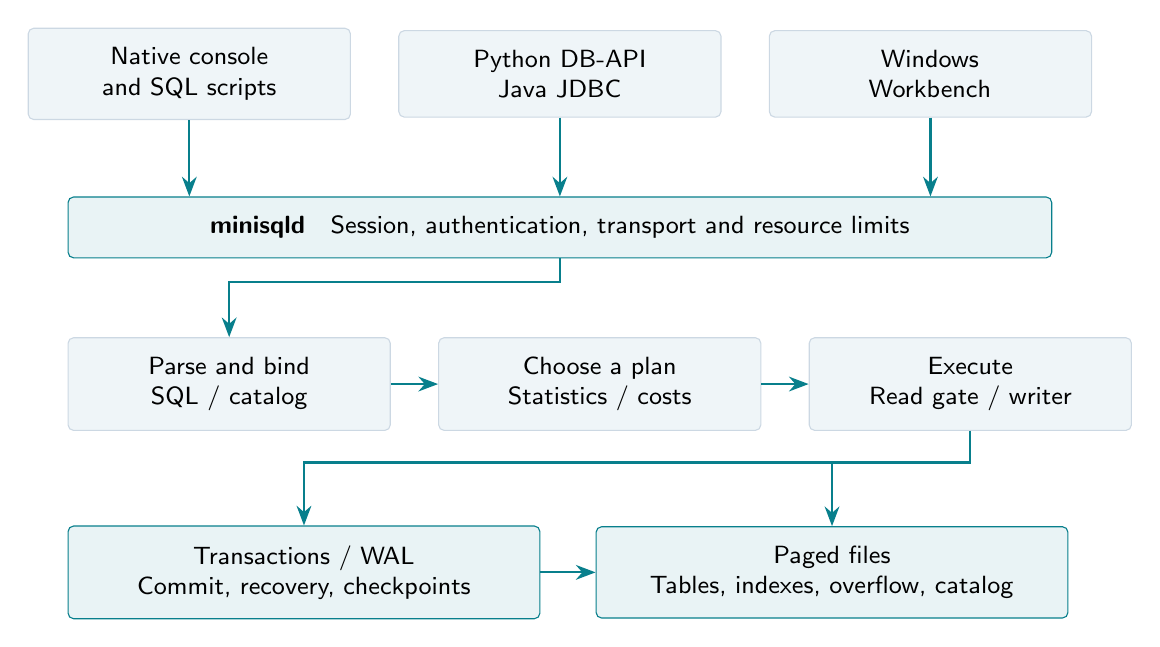
\begin{tikzpicture}[node distance=7mm and 6mm]
\node[box,text width=36mm] (shell) {Native console\\and SQL scripts};
\node[box,text width=36mm,right=of shell] (apps) {Python DB-API\\Java JDBC};
\node[box,text width=36mm,right=of apps] (gui) {Windows\\Workbench};
\node[strong,text width=120mm,below=10mm of apps] (server) {\textbf{minisqld}\quad Session, authentication, transport and resource limits};
\foreach \n in {shell,apps,gui}{\draw[arrow] (\n.south) -- (server.north -| \n.south);}
\node[box,text width=36mm,below=10mm of server.south west,anchor=north west] (sql) {Parse and bind\\SQL / catalog};
\node[box,text width=36mm,right=of sql] (plan) {Choose a plan\\Statistics / costs};
\node[box,text width=36mm,right=of plan] (execute) {Execute\\Read gate / writer};
\draw[arrow] (server.south) -- ++(0,-3mm) -| (sql.north);
\draw[arrow] (sql) -- (plan);\draw[arrow] (plan) -- (execute);
\node[strong,text width=55mm,below=12mm of sql.south west,anchor=north west] (wal) {Transactions / WAL\\Commit, recovery, checkpoints};
\node[strong,text width=55mm,right=7mm of wal] (files) {Paged files\\Tables, indexes, overflow, catalog};
\draw[arrow] (execute.south) -- ++(0,-4mm) -| (files.north);
\draw[arrow] (execute.south) -- ++(0,-4mm) -| (wal.north);
\draw[arrow] (wal) -- (files);
\end{tikzpicture}
\caption{MiniSQL's main components. Every client uses the server's SQL engine; the Workbench adds a user interface. Offline tools open a stopped database directly.}
\label{fig:architecture}
\end{figure}


The server is pointed at an already-created database directory. It does not
offer a SQL \code{CREATE DATABASE} or \code{USE database} workflow. Create a
database with \code{minisqld --init}; then start the server using the exact
directory printed by that command. Client connection paths such as
\code{/main} are protocol labels, not a way to switch the running server to
another disk database.

The directory contains authoritative catalog, table, index and WAL files as
well as metadata and derived acceleration files. Treat the database as a
whole. Copying an individual table file is not a supported way to export a
table, and renaming storage files is not the same as renaming SQL objects.
Offline tools take locks and expect the appropriate stopped-database state;
read their operation-specific instructions before running them.

\section{Durability, transactions and what an acknowledgement means}
\index{durability}\index{write-ahead log}
In autocommit mode, each successful data-changing statement has its own
transaction boundary. With an explicit transaction, you can perform several
changes and then \code{COMMIT} or \code{ROLLBACK}. MiniSQL uses a write-ahead
log (WAL), checksummed pages and recovery procedures. Committed work is
recovered using the engine's durable records; an arbitrary file copy made
while pages are changing is not a substitute for a backup procedure.

There are two different questions after a connection fails: did the server
commit the transaction, and did the application receive the reply? The
second can be false even when the first is true. An application that blindly
retries an order insertion can therefore create duplicate work. Use a stable
application identifier or unique key and a reconciliation query so you can
determine whether the operation already succeeded. This is an application
design rule, not a guarantee that a client can infer success from a lost
connection.

\section{A method for learning and diagnosing}
For each new feature, work through four questions: What result do I intend?
Which rows and keys represent it? Which MiniSQL syntax expresses it? How can
I verify the result? First run a \code{SELECT} that identifies the intended
rows. Then make the change inside a disposable transaction. Query the result
and either commit intentionally or roll back. Once correctness is established,
measure the plan and performance.

When an error occurs, preserve the smallest statement that reproduces it,
the relevant table definition, the source revision and the full error code
and text. Separate a parsing error from a constraint rejection, a connection
problem, an unsupported feature and damaged storage. The troubleshooting
chapter follows this distinction.

\tip{Checkpoint before continuing}{You should now be able to explain why
orders store a customer identifier, why order items need their own table,
why \code{NULL} differs from zero, and why a console connection is not the
database itself. The next chapter installs the programs; the guided tutorial
turns these ideas into a reproducible dataset.}
\sourcecode{src/apps/minisqld/main.ml}{Database initialization and the server's public modes.}
\sourcecode{src/minisql/client/console.ml}{A shell or script runs statements through one client session.}
\sourcecode{src/minisql/executor/dml.ml}{DML constraints and relationship validation.}

\chapter{Installation and database creation}
\label{ops:installation}

\section{Choose the implementation you intend to run}

MiniSQL is a native database server written in MiniLang. The server owns a
database directory; clients connect to its TCP listener and send SQL. The
command-line client is a separate program, so starting a client does not start
a server automatically. The native Windows Workbench is another client of the
same server. Python and Java applications can connect through the supplied
drivers.

This manual describes the development revision printed on its title page.
That revision uses database, table, index, and row format version 2. Its WAL
record framing remains version 1. The application version string and the
storage-format version answer different questions: a binary identifying
itself as MiniSQL 1.1.1 is not sufficient evidence that it can open a
particular database. Record the source revision and build target alongside
the executable.

\warning{Existing databases}{The current source rejects format-1 databases.
Do not point a newly built format-2 server at the only copy of an older
database. Retain the matching old executable, export the schema and data
through that executable, create a new database with the current executable,
and load the exported information. The page-size migration tool does not
implement a format-1 to format-2 conversion.}

\sourcecode{src/minisql/common/format_version.ml}{Persisted format identifiers.}
\sourcecode{docs/formats/FORMAT_COMPATIBILITY.md}{Compatibility policy for the current tree.}

\section{Platforms, prerequisites, and program inventory}
\index{installation}\index{Windows}\index{Linux}\index{build prerequisites}

The supported native targets are Windows x64 and Linux x64. Linux requires
glibc; native TLS requires OpenSSL 3, including \path{libssl.so.3} and
\path{libcrypto.so.3}. Windows uses Schannel and CryptoAPI for native TLS and
needs an operating-system configuration capable of the required TLS 1.3
profile. The Windows GUI is not a portable Linux application.

For a source build, use MiniLangCompilerPy or MiniLangCompilerML 1.3.0 or
newer, as required by the current repository. The Python compiler and the
repository's build/test tooling require Python 3.11 or newer. The Python
database connector itself has a separate Python 3.10 minimum. PowerShell is
needed for the supplied \path{build.ps1} launcher. A direct compiler command
can be used on Linux without that launcher.

\begin{longtable}{p{.27\linewidth}p{.66\linewidth}}
\toprule
Program & Purpose \\
\midrule
\endhead
\path{minisqld} & Creates databases, administers local passwords and encryption,
and runs the server. \\
\path{minisql} & Interactive SQL shell, single-query client, script runner,
and connection checks. \\
\path{minisql-check} & Opens a stopped database and verifies authoritative
storage, rows, overflow values, and indexes. \\
\path{minisql-backup} & Base backups, encrypted backups, restores, WAL archives,
point-in-time recovery, and standby administration. \\
\path{minisql-migrate} & Checks whether a page-size change is needed and
performs a separate offline copy-and-rewrite when requested. \\
\path{minisql-admin} & Windows-only graphical MiniSQL Workbench. \\
\bottomrule
\end{longtable}

Windows names end in \path{.exe}. Windows builds are placed in
\path{build/bin}; Linux builds are placed in \path{build/bin-linux} and omit
that suffix. Keep all programs from the same source revision together. A
checker or backup program is part of the storage implementation, so mixing
it with an unrelated server build is an unnecessary compatibility risk.

\sourcecode{build.ps1}{Target selection, compiler discovery, include paths, and executable inventory.}

\section{Build from source on Windows}
\index{build.ps1}\index{compiler}

Keep sibling checkouts for MiniSQL and the compiler. In PowerShell, change to
the MiniSQL repository and run:

\begin{lstlisting}
git clone https://github.com/MiniLangProject/MiniSQL.git
git clone https://github.com/MiniLangProject/MiniLangCompilerPy.git
cd MiniSQL
$compiler = "..\MiniLangCompilerPy\mlc_win64.py"
.\build.ps1 -Compiler $compiler -Target windows-x64 -AppsOnly
.\build\bin\minisqld.exe --version
\end{lstlisting}

The compiler path can be absolute. If \code{-Compiler} is omitted, the script
checks \code{MINILANG\_COMPILER} and several conventional repository-relative
locations. Explicit paths make a build easier to reproduce. Use
\code{-Python} to select a particular Python executable when more than one
is installed.

\begin{lstlisting}
.\build.ps1 -Compiler C:\Tools\MiniLangCompilerPy\mlc_win64.py `
  -Python C:\Python311\python.exe -Target windows-x64 -AppsOnly
\end{lstlisting}

With the native self-hosted compiler, supply its executable instead:

\begin{lstlisting}
.\build.ps1 -Compiler ..\MiniLangCompilerML\build\mlc_win64.exe `
  -Target windows-x64 -AppsOnly
\end{lstlisting}

The launcher discovers the compiler's \path{std/} include root and selects
its object pipeline for the large self-hosted build. \code{-AppsOnly} builds
the public programs; omitting it also compiles the native test applications.
\code{-Clean} removes the selected binary output directory before rebuilding.
The script verifies both the compiler's exit code and the existence of each
expected executable. A zero exit status from the compiler without an output
file is treated as failure.

Building Linux targets from the same checkout is possible by selecting
\code{-Target linux-x64}. Compiling a Linux ELF file does not execute its
tests on Windows; native execution requires Linux or an appropriate WSL
environment.

\section{Build and run on Linux}
\index{Linux!building}

If PowerShell is available on Linux, the same launcher can select
\code{linux-x64}. The following direct Python-compiler commands show the
equivalent source/include relationship without depending on PowerShell.
Run them from the MiniSQL repository with a sibling compiler checkout:

\begin{lstlisting}[language=bash]
mkdir -p build/bin-linux
compiler=../MiniLangCompilerPy/mlc_win64.py
compiler_root=../MiniLangCompilerPy
python3 "$compiler" src/apps/minisqld/main.ml \
  build/bin-linux/minisqld -I src -I "$compiler_root" \
  --target linux-x64
python3 "$compiler" src/apps/minisql/main.ml \
  build/bin-linux/minisql -I src -I "$compiler_root" \
  --target linux-x64
python3 "$compiler" src/apps/minisql_check/main.ml \
  build/bin-linux/minisql-check -I src -I "$compiler_root" \
  --target linux-x64
python3 "$compiler" src/apps/minisql_backup/main.ml \
  build/bin-linux/minisql-backup -I src -I "$compiler_root" \
  --target linux-x64
python3 "$compiler" src/apps/minisql_migrate/main.ml \
  build/bin-linux/minisql-migrate -I src -I "$compiler_root" \
  --target linux-x64
chmod +x build/bin-linux/minisql*
build/bin-linux/minisqld --version
\end{lstlisting}

The output remains native machine code: Python is a build dependency here,
not an interpreter that runs each SQL query. The optional monitoring,
replication, and qualification scripts use Python independently of the native
server.

If a generated program reports that a shared library cannot be loaded,
inspect the Linux runtime dependencies before changing SQL or database files.
If the compiler cannot find \code{std} modules, check the second include root.
If the shell reports permission denied for a compiled binary, check its
executable permission and the mount's execution policy.

\section{Create the first database}

\subsection{A database is created by the server tool}

MiniSQL does not implement SQL \code{CREATE DATABASE}, \code{DROP DATABASE},
or \code{USE}. A server instance is opened on one database path. Creating a
table in an existing database and creating that database directory are
different operations.

\begin{lstlisting}
# Windows PowerShell, from the repository root
.\build\bin\minisqld.exe --init .\data learning 4096
\end{lstlisting}

\begin{lstlisting}[language=bash]
# Linux, from the repository root
build/bin-linux/minisqld --init ./data learning 4096
\end{lstlisting}

The tool reports a generated path of the form
\path{data/db_<32-hexadecimal-digits>}, the logical name \code{learning},
and the page size. Copy the actual path from this output. The database is not
necessarily stored in a directory named \path{learning}; the UUID-derived
directory avoids confusing a logical database name with its physical identity.

Supported page sizes are 4096, 8192, 16384, and 32768 bytes. Omitting the last
argument selects 4096. Start with 4096 unless a measured workload gives a
reason to choose differently. Page size is persisted when the database is
created. Editing a JSON default later does not change existing pages.

The public \code{--init} command accepts the data root, logical name, and
optional page size. It uses the compiled default database settings. There is
no \code{--init-config} command that consumes arbitrary creation defaults
from JSON. Do not assume that a configuration file is read automatically.

\sourcecode{src/apps/minisqld/main.ml}{initializeDatabase and the --init argument branch.}
\sourcecode{src/minisql/catalog/catalog.ml}{Database creation and UUID-based paths.}

\subsection{Start a local learning server}

Replace the example path below with the path printed by initialization:

\begin{lstlisting}
$database = ".\data\db_REPLACE_WITH_THE_PRINTED_ID"
.\build\bin\minisqld.exe --serve $database 7432 32
\end{lstlisting}

\begin{lstlisting}[language=bash]
database='./data/db_REPLACE_WITH_THE_PRINTED_ID'
build/bin-linux/minisqld --serve "$database" 7432 32
\end{lstlisting}

The process remains running. Its startup banner reports the mode, physical
database path, address, port, connection limit, and request budget. This
particular mode binds to \code{127.0.0.1} and trusts local clients. Every
local client that can reach the port is administrative; a database password
does not protect this mode.

Open a second terminal in the repository and connect:

\begin{lstlisting}
.\build\bin\minisql.exe --ping 7432
.\build\bin\minisql.exe --shell 7432
\end{lstlisting}

On Linux the equivalents are \path{build/bin-linux/minisql --ping 7432} and
\path{build/bin-linux/minisql --shell 7432}. At the SQL prompt:

\begin{lstlisting}[language=SQL]
SELECT 2 + 3 AS answer;
SHOW TABLES;
\end{lstlisting}

The first query should return one row containing 5. A fresh database has no
user-created tables. The client session and the server process have separate
lifetimes: leaving the shell disconnects that client but keeps the server
running. To request a graceful stop from an authorized session, execute:

\begin{lstlisting}[language=SQL]
SHUTDOWN;
\end{lstlisting}

\sourcecode{src/apps/minisql/main.ml}{Client command forms.}
\sourcecode{src/apps/minisqld/main.ml}{Server mode selection and startup banner.}

\section{Choose a connection mode deliberately}

\begin{longtable}{p{.32\linewidth}p{.61\linewidth}}
\toprule
Server mode & Meaning and matching client family \\
\midrule
\endhead
\code{--serve} & Trusted loopback. Use \code{--shell}, \code{--query},
\code{--script}, or \code{--ping}. Appropriate for a local tutorial or an
environment whose local access is the intended trust boundary. \\
\code{--serve-authenticated} & Password-authenticated loopback with MiniSQL
protected framing after login. Use \code{--auth-shell-prompt} and the related
prompt commands. This mode is not TLS. \\
\code{--serve-secure} & MiniSQL-specific authenticated encrypted framing.
Use the \code{--secure-*} client family. This is a distinct protocol from TLS. \\
\code{--serve-tls} & Native TLS 1.3 plus database authentication. Use
\code{--tls-*} or \code{--tls-pin-*}. The certificate identity and trust
configuration must match. \\
\code{--serve-standby} & Read-only standby server, bound to loopback. This
requires a database materialized as a standby. \\
\bottomrule
\end{longtable}

Configuration-driven variants and fencing are explained later. The positional
\code{--serve-\allowbreak authenticated} fixes the address to loopback; the configured
authenticated listener has an explicit address from JSON and uses the same
MiniSQL-specific protected framing after authentication. Native TLS remains
the separate \code{--serve-tls} family. Match the client to the actual listener
mode rather than assuming that every encrypted listener speaks TLS.

\section{Organize an installation for repeatable operation}

Separate application binaries, database directories, configuration, keys,
logs, and backup destinations. Give the process write access to the database
and its intended logging/spill locations, read access to required certificates
and encryption keys, and no unnecessary permissions. Use absolute database,
configuration, log, and key paths in unattended launchers. Relative paths
resolve against the process working directory, which can differ between an
interactive shell and a service supervisor.

There is no universal installer wizard in the repository. Copying the native
binaries and supplying an explicit configuration is the deployment model.
The supplied systemd unit and Windows launch/stop scripts are templates to
adapt, not automatic account creation or service registration tools.

Keep a small installation record: source commit, compiler revision, target,
binary directory, database path and logical name, page size, listener mode,
port, configuration path, key-provider paths, and the date of the latest
successful restore drill. This information makes a later upgrade or incident
recovery concrete.

\section{Check the installation before loading important data}

At minimum, verify a query, a committed write, a restart, and an offline check.
Use a disposable database for these checks. A query result proves connection
and execution; a row that survives restart proves a more relevant path for
durable use. A checker result adds storage consistency evidence.

\begin{lstlisting}[language=SQL]
CREATE TABLE installation_check (
  id INTEGER PRIMARY KEY,
  note VARCHAR(80) NOT NULL
);
INSERT INTO installation_check VALUES (1, 'restart verification');
SELECT * FROM installation_check;
SHUTDOWN;
\end{lstlisting}

Run \path{minisql-check <database-path>} while the server is stopped. Start
the server again, query \code{installation\_check}, and confirm the row.
Drop this disposable table after the check if continuing to use the database.

For storage-format qualification, the repository provides a focused gate:

\begin{lstlisting}
.\test.ps1 -StorageV2 -Target windows-x64
.\test.ps1 -StorageV2 -Target linux-x64
\end{lstlisting}

Use the corresponding native host for execution. The direct Python runner
also supports \code{--compiler}, \code{--target}, selected cases,
\code{--integration}, and compile-only cross-target checks. The historical
106-phase release results belong to earlier validated revisions; they do not
automatically certify every new storage-format change. Consult the current
acceptance report and run the relevant gate for the binary being deployed.

\sourcecode{tests/run_storage_v2.py}{Focused storage-v2 compilation and execution gate.}
\sourcecode{docs/acceptance/STORAGE_V2_2026-11-24.md}{Recorded evidence and platform limits.}

\section{Troubleshooting the first connection}

\begin{longtable}{p{.29\linewidth}p{.64\linewidth}}
\toprule
Symptom & Check first \\
\midrule
\endhead
Connection refused & The server must still be running on the selected port.
The shell and server are different programs. \\
Database cannot be opened & Use the actual UUID directory, not only the data
root. Check permissions, the required encryption key, and whether another
process already owns the database lock. \\
Unsupported format & Confirm the source/build revision and persisted format.
Do not edit a header to bypass the check. \\
Authentication failure & Use the matching client mode, an enabled account,
the correct password, and a database \code{CONNECT} grant. \\
TLS handshake failure & Verify TLS 1.3 support, certificate/private-key
availability, the requested server name, and the trust or pin mode. \\
Handshake appears stuck in an older Windows daemon & Exit console selection
mode with Escape. Current code disables QuickEdit before logging, but an
already-running older process may still be paused by text selection. \\
\bottomrule
\end{longtable}

Do not troubleshoot a format or encryption error by deleting metadata, WAL,
lock files, or audit files. Preserve the directory and use the diagnostic
message to identify the failing boundary.

\chapter{Your first complete database}
\label{learn:tutorial}
\index{tutorial}
\learning{Create a fresh database, load a relational schema, insert data, retrieve useful answers, make reversible changes and verify the results. Every file in this chapter is supplied with the manual.}

\section{Prepare two terminals and one fresh database}
Complete the installation chapter first. Work from the repository root. Use
one terminal for the server and another for the client. In the first terminal
create a new teaching database:
\begin{lstlisting}[language=bash]
./build/bin-linux/minisqld --init ./data shop 4096
\end{lstlisting}
On Windows the equivalent command is:
\begin{lstlisting}[language=PowerShell]
.\build\bin\minisqld.exe --init .\data shop 4096
\end{lstlisting}
The output includes a directory beginning with \code{db\_}, a human-readable
database name and a page size. Copy the actual directory into the server
command. The following placeholder is deliberately not a real directory:
\begin{lstlisting}[language=bash]
./build/bin-linux/minisqld --serve ./data/db_<uuid> 7432 16
\end{lstlisting}
The server remains running. A listener-ready message means the server has
opened the database and reached its listener setup. Check the complete
startup output if the next command cannot connect.

In the second terminal, test the connection:
\begin{lstlisting}[language=bash]
./build/bin-linux/minisql --ping 7432
./build/bin-linux/minisql --shell 7432
\end{lstlisting}
\code{--ping} prints \code{PONG} on success. The shell displays a
\code{minisql>} prompt. The trusted listener is a local learning mode: its
sessions have administrative authority. Read the security chapter before
allowing users or applications to connect in a deployment.

\section{Understand the model before typing the schema}
The teaching database represents customers, products, orders and individual
order lines. A customer may have no orders. A product may have stock but no
orders. One order can contain several products. The schema retains these
distinctions instead of trying to fit all facts into one table.
\begin{figure}[htbp]
\centering
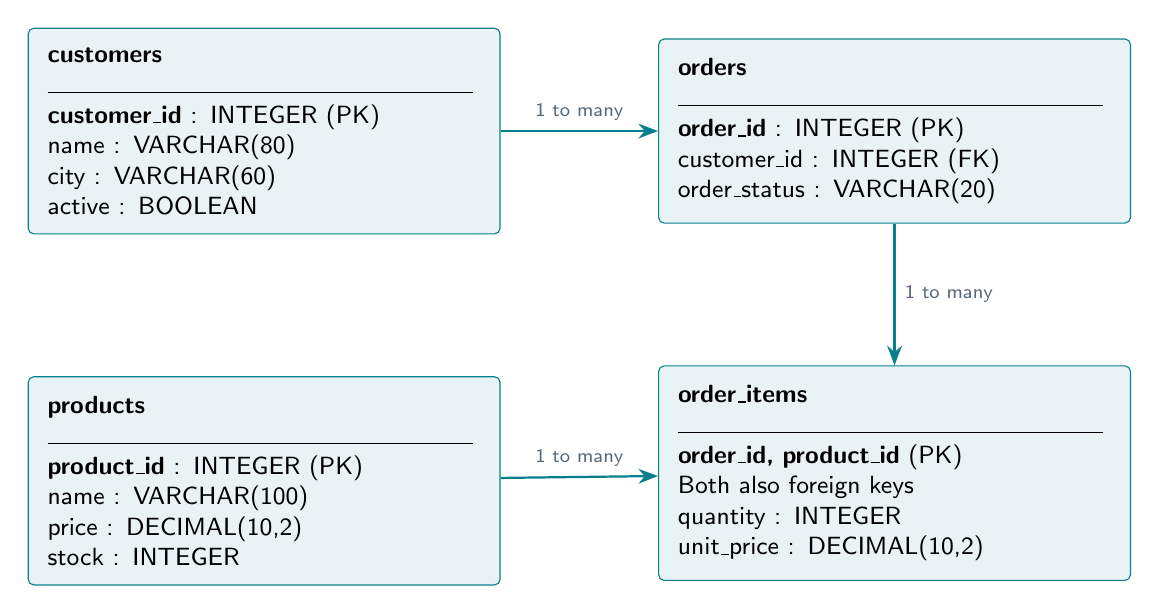
\begin{tikzpicture}[node distance=18mm and 20mm]
\node[strong,text width=55mm,align=left] (customers) {\textbf{customers}\\\rule{54mm}{.3pt}\\\textbf{customer\_id} : INTEGER (PK)\\name : VARCHAR(80)\\city : VARCHAR(60)\\active : BOOLEAN};
\node[strong,text width=55mm,align=left,right=of customers] (orders) {\textbf{orders}\\\rule{54mm}{.3pt}\\\textbf{order\_id} : INTEGER (PK)\\customer\_id : INTEGER (FK)\\order\_status : VARCHAR(20)};
\node[strong,text width=55mm,align=left,below=of customers] (products) {\textbf{products}\\\rule{54mm}{.3pt}\\\textbf{product\_id} : INTEGER (PK)\\name : VARCHAR(100)\\price : DECIMAL(10,2)\\stock : INTEGER};
\node[strong,text width=55mm,align=left,below=of orders] (items) {\textbf{order\_items}\\\rule{54mm}{.3pt}\\\textbf{order\_id, product\_id} (PK)\\Both also foreign keys\\quantity : INTEGER\\unit\_price : DECIMAL(10,2)};
\draw[arrow] (customers) -- node[smalllabel,above] {1 to many} (orders);
\draw[arrow] (orders) -- node[smalllabel,right] {1 to many} (items);
\draw[arrow] (products) -- node[smalllabel,above] {1 to many} (items);
\end{tikzpicture}
\caption{The teaching database: one customer can place many orders; order items connect orders to products. Keys are immutable in these examples.}
\label{fig:shop-schema}
\end{figure}


The examples use explicit stable identifiers so that expected results are
easy to compare. Identity and sequence features are taught later, with their
different allocation semantics. The identifier of an existing customer or
product is never changed during this tutorial.

\section{Create and populate the tables}
Leave the shell with \code{\textbackslash quit}, or open a third terminal,
and run the first script:
\begin{lstlisting}[language=bash]
./build/bin-linux/minisql --script 7432 \
  docs/manual/examples/01-create-shop.sql
\end{lstlisting}
On Windows:
\begin{lstlisting}[language=PowerShell]
.\build\bin\minisql.exe --script 7432 `
  .\docs\manual\examples\01-create-shop.sql
\end{lstlisting}
The file contains the following complete setup. It is intentionally designed
for a new empty database. Rerunning it on the same database should fail when
objects already exist; an unexpected pre-existing schema must not be silently
accepted as the tutorial schema.
\lstinputlisting[language=SQL,caption={The complete reproducible teaching database}]{examples/01-create-shop.sql}

The four \code{CREATE TABLE} statements are schema changes. They run before
the explicit transaction that loads data. The \code{BEGIN}/\code{COMMIT}
pair makes the initial row population one transaction. Parents are inserted
before children, so foreign-key checks can find the referenced rows.
\code{CHECK (stock >= 0)} prevents a negative quantity; \code{CHECK (quantity
> 0)} requires a positive order-line quantity. \code{NOT NULL} requires a
value rather than leaving it unknown.

The final count queries should report the following values:
\begin{table}[htbp]\centering
\caption{The teaching database after successful setup}
\begin{tabular}{l r l}\toprule
Table & Rows & What one row means\\\midrule
customers & 4 & One customer\\
products & 5 & One product offered for sale\\
orders & 4 & One order placed by a customer\\
order\_items & 6 & One product line in an order\\\bottomrule
\end{tabular}
\end{table}

\tip{What to do after a setup error}{Read the first error, not only the final
script status. A script stops at its failure point; earlier DDL may already
be committed. For the tutorial, create another fresh database instead of
guessing which objects to delete. The validation tool always uses a new
temporary directory.}

\section{Inspect rows and choose columns}
Reconnect with \code{--shell 7432} and run:
\begin{lstlisting}[language=SQL]
SELECT customer_id, name, city, active
FROM customers
ORDER BY customer_id;
\end{lstlisting}
\begin{table}[htbp]\centering
\caption{The four customers in identifier order}
\begin{tabular}{r l l l}\toprule
customer\_id & name & city & active\\\midrule
1 & Ada & London & TRUE\\
2 & Grace & New York & TRUE\\
3 & Linus & Helsinki & TRUE\\
4 & Margaret & NULL & FALSE\\\bottomrule
\end{tabular}
\end{table}
The selected column list controls the result's shape. It can omit columns,
reorder them or add expressions. A column alias such as
\code{COUNT(*) AS customer\_count} gives the result a readable heading.
Use explicit columns in application code so a later schema extension does
not accidentally change the expected result layout.

\section{Filter and sort}
\begin{lstlisting}[language=SQL]
SELECT product_id, name, stock
FROM products
WHERE stock < 15
ORDER BY stock, product_id;
\end{lstlisting}
The result contains Monitor Stand (104) with stock 8 and Mechanical Keyboard
(101) with stock 12, in that order. \code{WHERE} keeps rows for which its
condition is true. \code{ORDER BY stock, product\_id} sorts by stock, then
uses the identifier as a deterministic tie-breaker.

To find the two products with the most stock, reverse the first sort:
\begin{lstlisting}[language=SQL]
SELECT product_id, name, stock
FROM products
ORDER BY stock DESC, product_id
LIMIT 2;
\end{lstlisting}
The result is USB-C Cable (103, stock 100) followed by Notebook (105, stock
50). A bare \code{LIMIT 2} without \code{ORDER BY} would mean ``any first two
rows produced by the chosen plan'', not ``the two largest''.

\section{Work correctly with unknown values}
\begin{lstlisting}[language=SQL]
SELECT customer_id, name FROM customers
WHERE city IS NULL;

SELECT COUNT(city) AS known_cities,
       COUNT(*) AS customer_count
FROM customers;
\end{lstlisting}
Margaret is the customer with no recorded city. The counts are 3 known cities
and 4 customers. \code{COUNT(city)} counts non-null city values;
\code{COUNT(*)} counts rows. The test for an unknown value is
\code{IS NULL}, not \code{= NULL}. The language chapter develops the
three-valued logic behind this distinction.

\warning{NULL in the current text protocol}{The native console displays SQL
NULL as \code{NULL}. Protocol version 1 also uses that text for an actual
string containing the four characters \code{NULL}. The general Python/JDBC
result path consequently cannot distinguish them. Do not choose that literal
string as a special missing-data marker. This limitation is separate from
the engine's internal typed null representation.}

\section{Join related tables}
\begin{lstlisting}[language=SQL]
SELECT o.order_id, c.name, o.order_status
FROM orders o
JOIN customers c ON c.customer_id = o.customer_id
ORDER BY o.order_id;
\end{lstlisting}
\code{o} and \code{c} are table aliases. Qualified names such as
\code{o.customer\_id} make each column's origin clear. The join condition
matches an order's customer key to a customer row.

\begin{table}[htbp]\centering
\caption{Joining orders to their customers}
\begin{tabular}{r l l}\toprule
order\_id & name & order\_status\\\midrule
1001 & Ada & new\\
1002 & Grace & shipped\\
1003 & Ada & paid\\
1004 & Linus & new\\\bottomrule
\end{tabular}
\end{table}
Notice that Ada appears twice because she has two orders. A join produces
matching row combinations; it does not implicitly deduplicate customer
names. If a customer has no orders, an inner join omits that customer.

\section{Retain unmatched rows and count correctly}
\begin{lstlisting}[language=SQL]
SELECT c.name, COUNT(o.order_id) AS order_count
FROM customers c
LEFT JOIN orders o ON o.customer_id = c.customer_id
GROUP BY c.name
ORDER BY c.name;
\end{lstlisting}
The left join retains every customer. Margaret's unmatched right-hand
columns are null, so \code{COUNT(o.order\_id)} returns zero for her group.
The four results are Ada 2, Grace 1, Linus 1 and Margaret 0. Replacing
\code{COUNT(o.order\_id)} with \code{COUNT(*)} would count the retained
unmatched row as one. This is a common beginner mistake.

Names happen to be unique in this small fixture. In a real customer report,
group by the stable customer identifier as well as the display name, or two
different people with the same name could be merged into one group.

\section{Build a grouped business query}
\begin{lstlisting}[language=SQL]
SELECT c.name, SUM(i.quantity) AS units
FROM customers c
JOIN orders o ON o.customer_id = c.customer_id
JOIN order_items i ON i.order_id = o.order_id
GROUP BY c.name
HAVING SUM(i.quantity) >= 3
ORDER BY c.name;
\end{lstlisting}
This asks for customers whose orders contain at least three units in total.
The result is Ada 6 and Grace 3. \code{SUM(i.quantity)} adds integer
quantities within each customer's group. \code{HAVING} filters groups after
aggregation. \code{WHERE}, if present, would filter the input rows before
grouping. The total quantity across all six order lines is 10.
\begin{figure}[htbp]
\centering
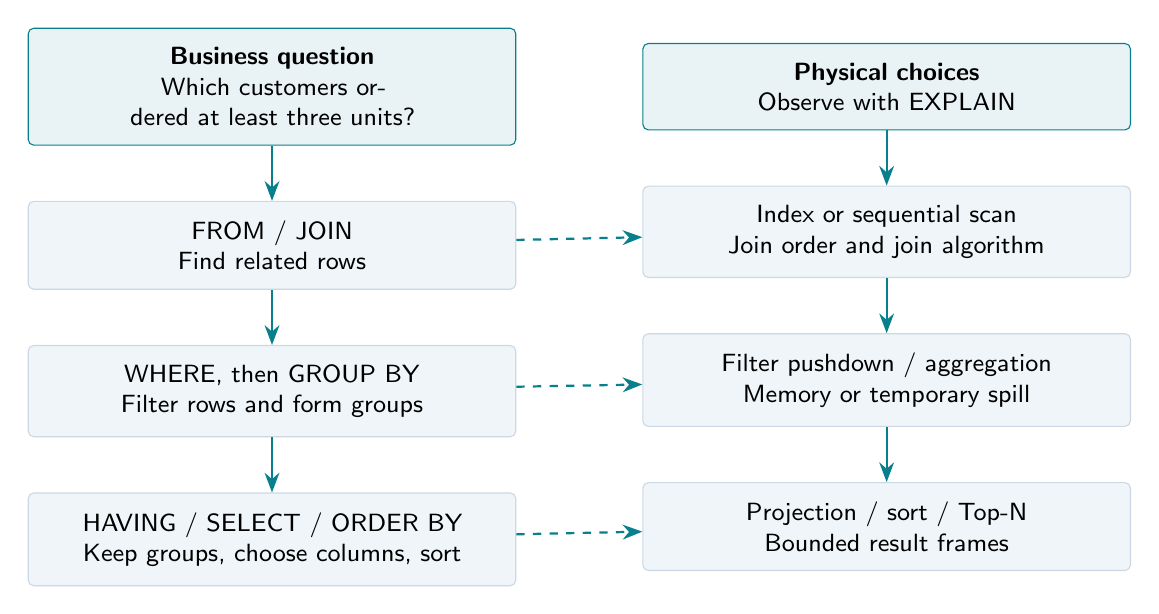
\begin{tikzpicture}[node distance=7mm and 16mm]
\node[strong,text width=57mm] (question) {\textbf{Business question}\\Which customers ordered at least three units?};
\node[strong,text width=57mm,right=of question] (physical) {\textbf{Physical choices}\\Observe with EXPLAIN};
\node[box,text width=57mm,below=of question] (sources) {FROM / JOIN\\Find related rows};
\node[box,text width=57mm,below=of physical] (access) {Index or sequential scan\\Join order and join algorithm};
\node[box,text width=57mm,below=of sources] (filter) {WHERE, then GROUP BY\\Filter rows and form groups};
\node[box,text width=57mm,below=of access] (blocking) {Filter pushdown / aggregation\\Memory or temporary spill};
\node[box,text width=57mm,below=of filter] (result) {HAVING / SELECT / ORDER BY\\Keep groups, choose columns, sort};
\node[box,text width=57mm,below=of blocking] (delivery) {Projection / sort / Top-N\\Bounded result frames};
\foreach \a/\b in {question/sources,sources/filter,filter/result,physical/access,access/blocking,blocking/delivery}{\draw[arrow] (\a) -- (\b);}
\draw[arrow,dashed] (sources) -- (access);\draw[arrow,dashed] (filter) -- (blocking);\draw[arrow,dashed] (result) -- (delivery);
\end{tikzpicture}
\caption{A learning model for a grouped query. SQL describes a result; the optimizer selects the physical work. This is a conceptual ordering, not a promise that every operator executes in the written order.}
\label{fig:query-thinking}
\end{figure}


\section{Interpret the price columns without assuming a wire format}
\begin{lstlisting}[language=SQL]
SELECT product_id, price FROM products WHERE product_id = 101;
\end{lstlisting}
At this revision the console returns \code{101 | 7990}. The declared scale is
2, so the stored coefficient 7990 represents the decimal value 79.90.
Exact decimal storage and exact decimal input validation are present, but
the generic wire formatter emits the coefficient without its decimal point.
The SQL arithmetic path also has a separate rescaling defect. For example,
the tested expression adding decimal 3.30 and 1.20 produces wire text 45000,
not a correct decimal sum representation.

The tutorial therefore uses integer quantities for SQL aggregation.
For an application that needs money calculations at this revision, one
workable design is to store and calculate integer minor units explicitly
(for example, cents), enforce a consistent scale in the application, and
format the result there. Range-check multiplication and sums. If reading an
existing \code{DECIMAL(10,2)} column, the application must know that column's
scale and decode its coefficient deliberately; ordinary result metadata does
not carry enough type information to reconstruct every value automatically.
Do not compensate for the arithmetic bug by guessing an extra divisor in
arbitrary SQL expressions.

\section{Make reversible changes}
Run the supplied transaction script:
\begin{lstlisting}[language=bash]
./build/bin-linux/minisql --script 7432 \
  docs/manual/examples/03-transactions.sql
\end{lstlisting}
Its first experiment is:
\begin{lstlisting}[language=SQL]
BEGIN;
UPDATE products SET stock = stock - 1 WHERE product_id = 101;
SAVEPOINT before_second;
UPDATE products SET stock = stock - 2 WHERE product_id = 101;
ROLLBACK TO before_second;
RELEASE before_second;
ROLLBACK;
\end{lstlisting}
The complete file queries the intermediate values. Stock starts at 12,
changes to 11, then 9, returns to 11 after the savepoint rollback, and returns
to 12 after the full rollback. A savepoint gives a named position within the
transaction; it does not commit earlier work. \code{RELEASE} removes that
savepoint. The final \code{ROLLBACK} abandons the transaction.

\begin{figure}[htbp]\centering
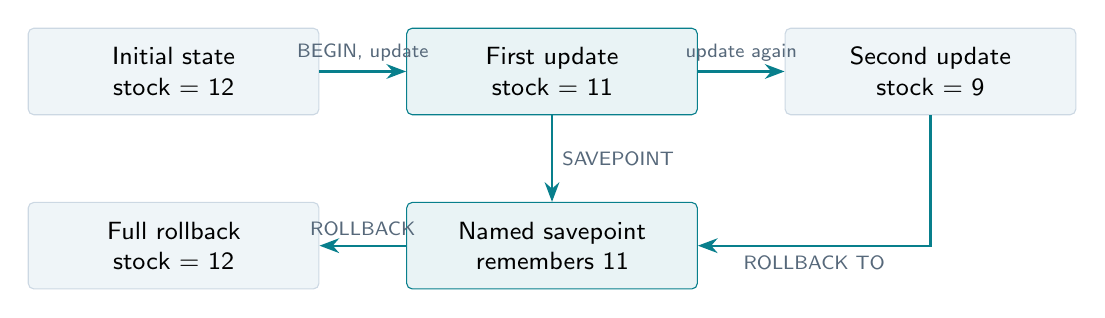
\begin{tikzpicture}[node distance=11mm and 11mm]
\node[box,text width=32mm] (initial) {Initial state\\stock = 12};
\node[strong,text width=32mm,right=of initial] (first) {First update\\stock = 11};
\node[box,text width=32mm,right=of first] (second) {Second update\\stock = 9};
\node[strong,text width=32mm,below=of first] (save) {Named savepoint\\remembers 11};
\node[box,text width=32mm,below=of initial] (rolled) {Full rollback\\stock = 12};
\draw[arrow] (initial) -- node[smalllabel,above] {BEGIN, update} (first);
\draw[arrow] (first) -- node[smalllabel,above] {update again} (second);
\draw[arrow] (first) -- node[smalllabel,right] {SAVEPOINT} (save);
\draw[arrow] (second.south) |- node[smalllabel,pos=.75,below] {ROLLBACK TO} (save.east);
\draw[arrow] (save) -- node[smalllabel,above] {ROLLBACK} (rolled);
\end{tikzpicture}
\caption{The tutorial's reversible stock experiment. Rolling back to a savepoint leaves the transaction active; a full rollback ends the transaction and restores its initial state.}
\label{fig:savepoints}
\end{figure}


Its second experiment inserts customer 99, updates the city, and deletes the
row, returning the changed values with \code{RETURNING}. A final rollback
leaves the teaching dataset unchanged. The check for customer 99 returns
zero rows counted. Read the transaction chapter before depending on failure,
DDL or concurrency behavior in application code.

\section{See constraints reject mistakes}
Run each of the following separately, outside an explicit transaction. Each
is an intentional error and is therefore not placed in the successful setup
script:
\begin{lstlisting}[language=SQL]
INSERT INTO customers(customer_id, name) VALUES (1, 'Duplicate');
INSERT INTO orders(order_id, customer_id, order_status)
VALUES (9999, 9999, 'new');
UPDATE products SET stock = -1 WHERE product_id = 101;
\end{lstlisting}
The first conflicts with an existing primary key. The second references a
customer that does not exist. The third violates the stock check. Query the
original rows afterwards to confirm that the rejected operations did not
perform the intended invalid change. In application code, treat a constraint
failure as a result to handle; do not convert every database error into
``try again forever''.

\section{Move to CTEs and window functions}
\path{examples/04-query-workshop.sql} gives named intermediate queries,
left-join anti-matching, per-customer order numbering, conditional display
values and a recursive sequence from 1 to 5. These build on the same schema.
The CTE that totals units per order returns 3, 3, 3 and 1 for orders
1001--1004. The window query numbers Ada's two orders 1 and 2 while restarting
at 1 for each other customer.

The query that finds customers without orders uses:
\begin{lstlisting}[language=SQL]
SELECT c.customer_id, c.name
FROM customers c
LEFT JOIN orders o ON o.customer_id = c.customer_id
WHERE o.order_id IS NULL
ORDER BY c.customer_id;
\end{lstlisting}
The result is Margaret (4). This uses an implemented, verified query shape.
The correlated-subquery section describes the narrower support and the
runtime issue found during validation; do not assume every standard
anti-join spelling is interchangeable in this development revision.

\section{Stop cleanly and reproduce your results}
When you have finished, issue \code{SHUTDOWN;} from the trusted shell. The
listener acknowledges the request, drains workers and closes its database.
You can then run offline tools on the directory. Reopen the same directory
with \code{--serve} to resume; do not run \code{--init} as a way of opening
an existing database.

To execute the tutorial in an isolated temporary database and compare its
results automatically, run:
\begin{lstlisting}[language=bash]
python3 docs/manual/tools/validate_examples.py \
  --bin-dir build/bin-linux \
  --output build/manual-validation.json
\end{lstlisting}
On Windows use \code{python}, the Windows binary directory, and normal
PowerShell line continuation if splitting the command. The runner starts
its own server on a free loopback port and removes its temporary database
afterwards. It does not open your teaching or application database.

\tip{You have completed the first learning milestone}{You can now create
and connect to a database, define relationships, load data, ask sorted and
grouped questions, retain unmatched rows, observe constraint errors and
undo a change. The next chapters explain each SQL feature systematically,
including syntax and MiniSQL-specific limitations.}
\sourcecode{src/minisql/sql/parser.ml}{The SQL parser and reserved-word behavior; the tutorial uses order\_status because STATUS is a keyword.}
\sourcecode{src/minisql/client/formatter.ml}{Result text formatting, including decimal coefficients.}
\sourcecode{src/minisql/executor/dml.ml}{Constraint checks and row changes used in the tutorial.}

\part{The MiniSQL SQL Language}
\chapter{SQL foundations: values, names, and expressions}
\label{sql:foundations}

SQL describes the result or change you want. A query does not tell MiniSQL which disk page to read first or which join algorithm to use. You name the data, describe relationships and conditions, and let the engine choose an executable plan. Understanding this distinction helps you write correct queries before trying to make them faster.

This chapter introduces the language shared by table definitions, queries, and data changes. Later chapters give complete statement forms. The reference describes the checked source revision, including places where accepted syntax has a narrower meaning than in another database.

\section{A statement, a script, and a session}

A statement is one instruction, such as a \code{SELECT} or \code{INSERT}. A script is a sequence of statements separated by semicolons. A session is the connection in which statements run; it owns transaction state, prepared statements, and the session's last sequence values. A second connection does not inherit that state.

\begin{lstlisting}[language=SQL]
SELECT 2 + 3 AS answer;
SELECT 'MiniSQL' AS product;
\end{lstlisting}

The first result has one column named \code{answer} and one value, 5. The second has one column named \code{product}. A \code{SELECT} without \code{FROM} evaluates a single conceptual input row, making it useful for learning expressions. \code{SELECT *} needs a source table; there are no columns to expand otherwise.

The parser accepts a final statement without a semicolon at end of input, but the interactive shell uses the terminator to decide when to submit accumulated input. Write terminators consistently in saved scripts. Repeated empty semicolon statements are ignored. A script containing several statements is not automatically one transaction: use an explicit transaction when the changes must succeed or fail together. A syntax error and a runtime error occur at different stages, so do not infer that earlier statements were undone merely because a later statement failed.

\sourcecode{src/minisql/sql/parser.ml}{parseTokens and parseStatement define statement boundaries and the accepted statement families.}

\section{Reading the syntax diagrams in this manual}

In reference listings, capital words are SQL keywords, lower-case names stand for your identifiers, square brackets mark optional syntax, braces with a vertical bar show alternatives, and an ellipsis means repetition. These notation characters are explanatory; they are not all typed literally. Parentheses shown in statement forms are literal SQL punctuation unless the surrounding explanation says otherwise.

For example:

\begin{lstlisting}[language=SQL]
SELECT [DISTINCT] expression [AS output_name] [, ...]
FROM table_name [AS alias]
[WHERE boolean_expression];
\end{lstlisting}

An actual statement might be:

\begin{lstlisting}[language=SQL]
SELECT customer_id, name AS customer_name
FROM customers
WHERE active = TRUE;
\end{lstlisting}

SQL result rows have no guaranteed order unless the query specifies \code{ORDER BY}. Physical insertion order, primary-key order, and the order printed by an earlier run are not substitutes for an ordering clause.

\section{Keywords, identifiers, quoting, and comments}
\index{identifiers}\index{reserved words}\index{quoting}\index{comments}

\subsection{Names and letter case}

Keywords are case-insensitive. Unquoted identifiers are normalized using ASCII lowercasing, so \code{CUSTOMERS}, \code{Customers}, and \code{customers} refer to the same ordinary name. Double-quoted identifiers preserve spelling and case. Single quotes delimit string values, not identifiers.

\begin{lstlisting}[language=SQL]
CREATE TABLE name_example (
    id INTEGER PRIMARY KEY,
    "DisplayName" VARCHAR(60)
);
INSERT INTO name_example(id, "DisplayName")
VALUES (1, 'Ada''s account');
SELECT "DisplayName" FROM name_example;
\end{lstlisting}

The value contains one apostrophe: \code{Ada's account}. Double a single quote inside a string and double a double quote inside a quoted identifier. Backticks, bracketed identifiers, and backslash string escapes are not alternative quoting conventions in this grammar.

An unquoted identifier begins with a letter, underscore, or non-ASCII UTF-8 byte; subsequent characters may also include digits and a dollar sign. Prefer short ASCII names with underscores for portable scripts and persisted expression definitions. Some words, particularly data-type and built-in function names, are contextual keywords and remain usable as identifiers. Grammar words such as \code{SELECT}, \code{WHERE}, and \code{ORDER} should be avoided as ordinary names.

\warning{Quoted names and persisted expressions}{Quoted identifiers work in ordinary SQL, but the current functional-index persistence check rejects names whose meaning would change after formatting and reparsing. Choosing simple lower-case names avoids this limitation and makes scripts easier to maintain.}

\subsection{Schemas and qualification}

The ordinary schema is \code{public}. \code{customers} and \code{public.customers} name the same table. An object in another schema uses a two-part name, for example \code{sales.orders}. Column references can use a table alias, such as \code{o.order\_id}. Three-part catalog names and configurable search paths are not implemented. A database is selected when the server or connection is opened; there is no \code{USE database} statement.

\begin{lstlisting}[language=SQL]
SELECT c.customer_id, c.name
FROM public.customers AS c
WHERE c.active = TRUE;
\end{lstlisting}

After introducing an alias, use it consistently. When two sources have a column with the same name, qualify the reference to avoid ambiguity.

\subsection{Comments and whitespace}

Whitespace can separate tokens across lines. The lexer supports line comments introduced by two hyphens and block comments delimited by slash-star and star-slash.

\begin{lstlisting}[language=SQL]
-- Find active customers.
SELECT customer_id, name
FROM customers
/* Add more filters here when required. */
WHERE active = TRUE;
\end{lstlisting}

Block comments are not nested. A terminator inside a quoted string is part of that string, not the end of the statement. Keep explanatory comments separate from data literals when building scripts in another language.

\sourcecode{src/minisql/sql/lexer.ml}{skipIgnored, readIdentifier, readQuotedIdentifier, and the string scanner define the lexical rules.}
\sourcecode{src/minisql/sql/dialect.ml}{keywordList, nonReservedIdentifierKeywordList, and canonicalIdentifier provide the exact keyword policy.}

\section{Literal values and explicit conversion}
\index{literals}\index{CAST}\index{type conversion}

\begin{longtable}{p{.25\linewidth}p{.68\linewidth}}
\toprule
Form & Meaning and practical rule \\
\midrule
\endhead
\code{42}, \code{-7} & Integer literals. Unary signs are parsed as operators. Large positive integer tokens can use the full stored BIGINT representation, but arithmetic and negative boundary expressions have additional runtime limits. \\
\code{3.3}, \code{1.25e2} & Approximate-number literals, normally bound as DOUBLE. The decimal separator is a dot. INSERT into DECIMAL uses target-directed exact literal conversion. \\
\code{'hello'} & A string value. Two adjacent quotes inside it represent one quote. An empty string is distinct from NULL. \\
\code{TRUE}, \code{FALSE} & Boolean values. Conditions require Boolean expressions; an arbitrary integer is not a truth value. \\
\code{NULL} & An absent or unknown value, not zero, an empty string, or the string \code{'NULL'}. \\
\code{?} & A positional parameter in a prepared statement. It represents a value, never a table name, keyword, or arbitrary SQL fragment. \\
\code{CURRENT\_TIMESTAMP} & Recognized by the grammar, but the checked implementation binds an epoch-zero placeholder. Do not use it to record the current time. \\
\bottomrule
\end{longtable}

Use \code{CAST(expression AS type)} for a deliberate conversion:

\begin{lstlisting}[language=SQL]
SELECT CAST('42' AS INTEGER) AS answer;
SELECT CAST(7 AS VARCHAR(8)) AS number_as_text;
SELECT CAST('TRUE' AS BOOLEAN) AS enabled;
SELECT CAST('3.30' AS DECIMAL(10,2)) AS amount;
\end{lstlisting}

The first three logical values are integer 42, text \code{'7'}, and Boolean true. The last value is stored exactly at scale two; the current text formatter prints its scaled coefficient, 330. This display limitation and the more serious DECIMAL-expression limitations are explained in Chapter~\ref{sql:schema}.

Assignment conversion is stricter than explicit casting. A quoted string is not silently accepted for every numeric column. The text-to-number cast validates spelling and overflow. Numeric-to-Boolean casts accept only 0 and 1; text-to-Boolean casts accept case-insensitive \code{TRUE}/\code{FALSE} and the strings \code{'1'}/\code{'0'}. A cast is not a general-purpose date parser: ISO dates and times in strings are not parsed by the present temporal conversion code.

There are no SQL binary literals such as \code{X'ABCD'}, no array literal, and no JSON data type. BINARY, VARBINARY, and BLOB exist in the engine, but the SQL text interface cannot currently construct a non-NULL binary value from a binary literal. A connector's existence does not imply that it supplies typed binary parameters.

\sourcecode{src/minisql/sql/values.ml}{fromLiteral, literalInteger, decimalWordsFromText, convert, and cast define literal and conversion behavior.}
\sourcecode{src/minisql/client/formatter.ml}{valueText exposes scalar and Int64Words values as protocol text.}

\section{NULL and three-valued logic}
\index{NULL}\index{three-valued logic}
\label{sql:null}

SQL conditions have three possible logical outcomes: true, false, and unknown. A comparison involving NULL normally yields unknown. A \code{WHERE} clause retains only rows for which its condition is true. Both false and unknown are filtered out.

\begin{lstlisting}[language=SQL]
SELECT customer_id, name
FROM customers
WHERE city IS NULL;

SELECT customer_id, name
FROM customers
WHERE city IS NOT NULL;
\end{lstlisting}

Do not write \code{city = NULL}. That asks for a comparison with an unknown value. Use the dedicated \code{IS NULL} predicate. NULL also propagates through ordinary arithmetic and text concatenation.

\begin{longtable}{p{.25\linewidth}p{.20\linewidth}p{.20\linewidth}p{.23\linewidth}}
\toprule
Left & Right & AND & OR \\
\midrule
\endhead
TRUE & TRUE & TRUE & TRUE \\
TRUE & FALSE & FALSE & TRUE \\
TRUE & UNKNOWN & UNKNOWN & TRUE \\
FALSE & FALSE & FALSE & FALSE \\
FALSE & UNKNOWN & FALSE & UNKNOWN \\
UNKNOWN & UNKNOWN & UNKNOWN & UNKNOWN \\
\bottomrule
\end{longtable}

The table is symmetric: exchanging the operands does not change the logical result. \code{NOT TRUE} is false, \code{NOT FALSE} is true, and \code{NOT UNKNOWN} is unknown. The evaluator short-circuits Boolean AND after a false left operand and OR after a true left operand.

The truth-test predicates always produce a non-NULL Boolean result:

\begin{lstlisting}[language=SQL]
SELECT TRUE IS TRUE AS a,
       FALSE IS NOT TRUE AS b,
       CAST(NULL AS BOOLEAN) IS UNKNOWN AS c;
\end{lstlisting}

All three values are true. Supported forms are \code{IS [NOT] TRUE}, \code{IS [NOT] FALSE}, and \code{IS [NOT] UNKNOWN}. Parenthesize a compound condition before attaching a truth test:

\begin{lstlisting}[language=SQL]
SELECT customer_id
FROM customers
WHERE (city = 'Berlin') IS UNKNOWN;
\end{lstlisting}

\subsection{CHECK differs from WHERE}

A \code{CHECK} constraint rejects false; true and unknown pass. Therefore \code{CHECK (quantity > 0)} does not by itself prohibit NULL. Write \code{quantity INTEGER NOT NULL CHECK (quantity > 0)} when every row must have a positive quantity. This distinction is central to reliable schema design.

\subsection{Replacing an absent value}

\code{COALESCE} returns the first non-NULL argument. Use a compatible fallback type:

\begin{lstlisting}[language=SQL]
SELECT name, COALESCE(city, 'Not recorded') AS city_label
FROM customers;
\end{lstlisting}

The original column remains NULL in the table; only the result is replaced. A display replacement should not be confused with a data correction. To store a replacement, issue an explicit \code{UPDATE}.

\warning{NULLIF implementation difference}{The current scalar evaluator propagates any NULL argument before its NULLIF-specific comparison. Consequently \code{NULLIF(5, NULL)} produces NULL in this revision. This differs from the usual SQL behavior. Use an explicit CASE expression when the second argument may be NULL and retaining the first value matters.}

\sourcecode{src/minisql/sql/values.ml}{truth, logicalAnd, logicalOr, and logicalNot implement three-valued logic.}
\sourcecode{src/minisql/sql/expressions.ml}{predicatePasses, checkPasses, and evaluateScalarValues distinguish filtering, CHECK, and scalar NULL handling.}

\section{Operators and precedence}
\index{operators}\index{operator precedence}

\begin{longtable}{p{.25\linewidth}p{.68\linewidth}}
\toprule
Binary group, weakest first & Operators and interpretation \\
\midrule
\endhead
Boolean alternative & \code{OR}. At least one condition must be true. \\
Boolean conjunction & \code{AND}. Both conditions must be true. \\
Comparisons & \code{=}, \code{<>}, \code{!=}, \code{<}, \code{<=}, \code{>}, \code{>=}. Operands must have compatible types. \\
Text concatenation & \code{||}. Both operands must be text. NULL yields NULL. \\
Additive arithmetic & \code{+}, \code{-}. Numeric operands only. \\
Multiplicative arithmetic & \code{*}, \code{/}, \code{\%}. Numeric operands only; zero divisors are errors. \\
\bottomrule
\end{longtable}

Within a binary precedence group, evaluation is left-associative. Parentheses override grouping. Unary \code{+}, unary \code{-}, and \code{NOT} are parsed tightly. Predicate suffixes such as \code{IS NULL}, \code{LIKE}, \code{IN}, and \code{BETWEEN} are attached during primary-expression parsing. This is not an exact copy of every other SQL dialect's precedence table.

\begin{lstlisting}[language=SQL]
SELECT 2 + 3 * 4 AS a, (2 + 3) * 4 AS b;
-- a = 14, b = 20

SELECT customer_id
FROM customers
WHERE active = TRUE AND (city = 'Berlin' OR city = 'Bonn');
\end{lstlisting}

Always write \code{NOT (stock > 0)} when negating a comparison. For a computed left operand, write \code{(stock + 1) BETWEEN 2 AND 5} or \code{(name || '!') LIKE 'A\%'}. Parentheses make the intended predicate boundary unambiguous in this parser.

Mixed numeric types use a common type. The numeric rank increases from SMALLINT through INTEGER, BIGINT, DECIMAL, REAL, and DOUBLE. This ranking does not promise complete scale-aware DECIMAL mathematics or arbitrary-precision arithmetic. Division always binds a DOUBLE result, so \code{SELECT 5 / 2} returns 2.5. Assignment of a fractional result back into an integral column is a separate conversion and must not be assumed to truncate safely. See the type caveats before building accounting logic.

String comparison is lexicographic over UTF-8 bytes and case-sensitive. There is no configurable collation, accent-insensitive comparison, or Unicode case-folding locale. CHAR values are padded with spaces to their declared byte width; trailing spaces remain part of their stored string. Normalize values deliberately if comparison should ignore superficial differences.

\sourcecode{src/minisql/sql/parser.ml}{operatorPrecedence, parseUnary, parsePredicateTail, and parseExpression define the actual grouping rules.}
\sourcecode{src/minisql/sql/types.ml}{commonNumeric and comparable define type combination and comparison eligibility.}
\sourcecode{src/minisql/sql/expressions.ml}{numericResult and comparisonResult execute operators.}

\section{Predicates for finding the right rows}

\subsection{Ranges with BETWEEN}
\index{BETWEEN}

\begin{lstlisting}[language=SQL]
SELECT product_id, name, stock
FROM products
WHERE stock BETWEEN 5 AND 20;
\end{lstlisting}

Both endpoints are included. The expression means \code{stock >= 5 AND stock <= 20}. \code{NOT BETWEEN} negates the test. A NULL operand or endpoint produces unknown unless the underlying three-valued conjunction can determine a false result. For a range with an exclusive upper bound, write the two comparisons explicitly.

\subsection{Membership with IN}
\index{IN}\index{NOT IN}

\begin{lstlisting}[language=SQL]
SELECT order_id, order_status
FROM orders
WHERE order_status IN ('new', 'paid');
\end{lstlisting}

The list must contain at least one value. \code{NOT IN} is useful only when its NULL behavior is understood. If no value matches and the candidate list contains NULL, the result is unknown rather than true. Thus \code{2 NOT IN (1, NULL)} does not pass a filter. For the current native implementation, use a LEFT JOIN followed by an IS NULL test on the non-nullable joined key when checking for absent related rows. A verified defect in correlated NOT EXISTS is described in Section~\ref{sql:subqueries}.

\subsection{Patterns with LIKE}
\index{LIKE}

\begin{lstlisting}[language=SQL]
SELECT customer_id, name
FROM customers
WHERE name LIKE 'A%';
\end{lstlisting}

Percent matches zero or more bytes. Underscore matches one byte. The matching engine is case-sensitive and operates on UTF-8 bytes; an underscore is not guaranteed to match one non-ASCII character. Common prefix, suffix, and contains patterns have optimized byte-search paths, while the general matcher uses bounded-memory wildcard matching.

\begin{longtable}{p{.25\linewidth}p{.68\linewidth}}
\toprule
Pattern & Matches \\
\midrule
\endhead
\code{'Mini\%'} & Any text beginning with \code{Mini}. \\
\code{'\%SQL'} & Any text ending with \code{SQL}. \\
\code{'\%shop\%'} & Text containing the byte sequence \code{shop}. \\
\code{'A\_'} & An ASCII A followed by exactly one byte. \\
\bottomrule
\end{longtable}

\code{NOT LIKE} is supported. There is no \code{ESCAPE} clause and no regular-expression operator. If percent or underscore is ordinary data that must match literally, do not assume that a backslash escapes it; use equality or perform the more specialized matching in the application.

\sourcecode{src/minisql/sql/expressions.ml}{likeResult, evaluateIn, evaluateBetween, and evaluateTruthTest implement these predicates.}
\sourcecode{src/tests/m36_predicates_fetch.ml}{Regression examples cover IN, BETWEEN, truth tests, NOT LIKE, NULL-sensitive NOT IN, and FETCH.}

\section{CASE: choosing an output value}
\index{CASE}

A searched CASE evaluates conditions in order and chooses the first true branch. A simple CASE compares one operand with each WHEN value. If no branch matches and no ELSE is present, the result is NULL. Branch result types must be compatible.

\begin{lstlisting}[language=SQL]
SELECT product_id, name,
       CASE
         WHEN stock = 0 THEN 'out of stock'
         WHEN stock < 5 THEN 'low stock'
         ELSE 'available'
       END AS stock_state
FROM products;

SELECT order_id,
       CASE order_status
         WHEN 'new' THEN 'Awaiting payment'
         WHEN 'paid' THEN 'Ready to ship'
         ELSE 'Other state'
       END AS next_action
FROM orders;
\end{lstlisting}

CASE returns a value; it does not execute SQL statements or provide procedural branching. The chosen result branch is evaluated at runtime, but all branches must still be valid and type-compatible when the query is bound. An unreachable branch is not a way to hide an unknown column.

\tip{A disciplined query-writing routine}{First identify the source and the required row set. Write the WHERE clause, inspect a small ordered sample, then add computed columns. Add aggregation only after verifying the input rows. Keep explicit aliases for calculated columns so client code does not depend on automatically formatted expression names.}

\section{Check your understanding}

Before continuing, be able to explain why \code{city IS NULL} is different from \code{city = NULL}; why a primary key does not imply result order; why \code{CHECK (stock >= 0)} still needs NOT NULL if absence is forbidden; and why a parameter cannot stand in for a table name. Write a query that lists active customers whose city is either Berlin or Bonn, and another that gives an explicit label to customers without a city. The important result is a correct set of rows, not a particular physical execution plan.

\chapter{Designing schemas, tables, types, and indexes}
\label{sql:schema}

A schema translates an application's rules into durable structure. It answers four questions: what constitutes one row, how a row is identified, which values are allowed, and how rows refer to one another. Good SQL begins with those decisions. The database can enforce many of them, but the current implementation has specific boundaries that must be understood before relying on an apparently familiar keyword.

\section{From a business fact to a table}

The tutorial store separates customers, products, orders, and order items. A customer's name belongs in the customer row; an order refers to that customer by an identifier. An order can contain several products, and a product can occur in several orders, so a separate order-item table represents that many-to-many relationship. Its quantity describes one product in one order.

This avoids repeating the customer address in every product row or storing a comma-separated list of product identifiers inside an order. Repetition creates update anomalies: one copy is changed while another remains stale. A list inside a string loses ordinary relational checks and requires application parsing. Columns should contain individual values appropriate to their declared types.

A primary key identifies one row. A foreign key records a relationship. A unique constraint prevents duplicate candidate keys. NOT NULL requires a value; CHECK adds a row-level condition. An index is a physical access structure that may speed queries and can also implement uniqueness. These concepts are related, but they solve different problems.

\section{Create and remove a schema}
\index{schema}\index{CREATE SCHEMA}\index{DROP SCHEMA}

\begin{lstlisting}[language=SQL]
CREATE SCHEMA [IF NOT EXISTS] schema_name;
DROP SCHEMA [IF EXISTS] schema_name [RESTRICT];
\end{lstlisting}

\begin{lstlisting}[language=SQL]
CREATE SCHEMA IF NOT EXISTS reporting;
CREATE TABLE reporting.daily_count (
    day_number INTEGER PRIMARY KEY,
    order_count INTEGER NOT NULL CHECK (order_count >= 0)
);
\end{lstlisting}

The built-in schemas \code{public} and \code{information\_schema} always exist. An omitted schema means public. There is no session search-path configuration and no cross-database three-part qualification. DROP SCHEMA is restrictive: remove its objects before dropping it. There is no schema CASCADE shortcut in this grammar.

Use separate schemas to clarify ownership or purpose, not as an assumption about independent database files or independent transaction domains. A schema is a namespace inside the open database. Administrative database creation uses the server's initialization command, not \code{CREATE DATABASE} SQL.

\sourcecode{src/minisql/sql/parser.ml}{parseCreateSchema, parseDrop, and parseObjectName define schema syntax and qualification.}
\sourcecode{src/minisql/executor/executor.ml}{Schema DDL and INFORMATION\_SCHEMA execution enforce the database namespace rules.}

\section{The complete CREATE TABLE form}
\index{CREATE TABLE}

\begin{lstlisting}[language=SQL]
CREATE TABLE [IF NOT EXISTS] [schema_name.]table_name (
    column_name data_type [column_attribute ...],
    ...
    [table_constraint, ...]
);
\end{lstlisting}

At least one column is required. Column names must be distinct. A column attribute can specify NULL or NOT NULL, DEFAULT, a primary or unique key, CHECK, a reference, an identity, or a stored generated expression. Table constraints express multi-column keys and explicitly named rules.

\begin{lstlisting}[language=SQL]
CREATE TABLE inventory_example (
    item_id INTEGER PRIMARY KEY,
    sku VARCHAR(30) NOT NULL,
    label VARCHAR(100) NOT NULL,
    stock INTEGER NOT NULL DEFAULT 0,
    active BOOLEAN NOT NULL DEFAULT TRUE,
    CONSTRAINT uq_inventory_sku UNIQUE (sku),
    CONSTRAINT ck_inventory_stock CHECK (stock >= 0)
);
\end{lstlisting}

The named constraints make later maintenance readable. IF NOT EXISTS suppresses the conflict caused by an existing name; it does not compare the existing schema with the requested definition. A deployment script should inspect metadata or maintain its own schema version instead of treating an idempotent CREATE as a migration verifier.

There is no \code{CREATE TABLE AS SELECT}, temporary-table declaration, table inheritance, partitioning syntax, or table-level storage-engine selector. Create the desired table explicitly, then use INSERT SELECT to populate it. Tables do not have an implicit user-visible row identifier: define your own key.

\sourcecode{src/minisql/sql/parser.ml}{parseCreateTable, parseColumnDefinition, and parseTableConstraint define the table grammar.}
\sourcecode{src/minisql/sql/binder.ml}{bindCreateTable validates duplicate names, types, identity counts, and generated-column references.}

\section{Choosing a data type}
\index{data types}\index{BIGINT}\index{BINARY}\index{BLOB}\index{BOOLEAN}\index{CHAR}\index{DATE}\index{DECIMAL}\index{DOUBLE}\index{INTEGER}\index{REAL}\index{SMALLINT}\index{TEXT}\index{TIME}\index{TIMESTAMP}\index{VARBINARY}\index{VARCHAR}
\label{sql:types}

\begin{longtable}{p{.25\linewidth}p{.68\linewidth}}
\toprule
Type & Meaning and limits in this implementation \\
\midrule
\endhead
BOOLEAN & TRUE, FALSE, or NULL if nullable. An integer column is not a substitute for a Boolean predicate. \\
SMALLINT & Signed 16-bit integer: -32,768 through 32,767. Overflow is rejected. \\
INTEGER, INT & Signed 32-bit integer: -2,147,483,648 through 2,147,483,647. INT is an alias. \\
BIGINT & Signed 64-bit storage using a high/low-word representation. Full-width values can be stored and compared, but not every scalar arithmetic or text-formatting path supports the entire range. \\
REAL & Approximate numeric value. Storage format 2 stores it as IEEE-754 binary64, not a 32-bit float. \\
DOUBLE, DOUBLE PRECISION, FLOAT & Approximate binary64 numeric value; FLOAT maps to DOUBLE. No user-selected FLOAT precision is implemented as a separate storage class. \\
DECIMAL(p,s), NUMERIC(p,s) & Exact scaled integer input and storage, with \(1\leq p\leq18\), \(0\leq s\leq p\). Bare DECIMAL defaults to precision 18, scale 0. The computation and display caveats below are essential. \\
CHAR(n) & Text bounded by n UTF-8 bytes and padded with ASCII spaces to exactly n bytes. A positive length is required. \\
VARCHAR(n) & Text bounded by n UTF-8 bytes without padding. A positive length is required. \\
TEXT & Variable-size text, with overflow storage for large values. Resource and storage limits still apply. \\
BINARY(n) & Exactly n bytes. A short value is rejected rather than zero-padded. SQL text has no binary-literal syntax. \\
VARBINARY(n) & Up to n bytes. A positive length is required. The same input-interface limitation applies. \\
BLOB & Variable-size binary data, including overflow storage. Ordinary SQL text and current connector parameters do not provide a general non-NULL binary input path. \\
DATE & Signed integer count of days relative to 1970-01-01. Current temporal conversion does not parse ISO date strings. \\
TIME[(p)] & Signed 64-bit microsecond representation for time of day; precision parameter 0 through 6 is accepted. \\
TIMESTAMP[(p)] & Signed 64-bit microsecond count relative to the Unix epoch; precision parameter 0 through 6 is accepted. No timezone-qualified SQL type exists. \\
\bottomrule
\end{longtable}

Type spelling matters at the grammar boundary. Use the documented keyword spellings, including BOOLEAN. Although an internal type helper mentions BOOL, BOOL is not a normal recognized type keyword in the current lexer and should not be used as a portable alias.

\subsection{Text length is a byte limit}

A VARCHAR declaration limits encoded bytes, whereas LENGTH and CHAR\_LENGTH count UTF-8 character starts. ASCII characters use one byte, but many other characters use two or more. A column declared VARCHAR(5) cannot necessarily hold five displayed characters. Combining marks and multi-code-point emoji make a visual character count an additional, different concept.

Choose lengths from the actual encoding and application constraints. Do not use CHAR to obtain case-insensitive matching or automatic trimming: its padding remains part of the value. Use TRIM explicitly when removing surrounding ASCII spaces is appropriate. MiniSQL does not provide locale collations or Unicode normalization.

\subsection{Exact DECIMAL input does not imply correct DECIMAL calculations}
\label{sql:decimal-caveat}

DECIMAL(p,s) stores an integer coefficient with an implied scale. For DECIMAL(10,2), logical 3.30 is represented by coefficient 330. The insertion path can preserve the spelling of a numeric literal and convert it exactly. Excess nonzero fractional digits and precision overflow are errors, not silently rounded values.

\begin{lstlisting}[language=SQL]
CREATE TABLE decimal_demo (
    id INTEGER PRIMARY KEY,
    amount DECIMAL(10,2) NOT NULL
);
INSERT INTO decimal_demo(id, amount) VALUES (1, 3.30);
-- Rejected: a nonzero third fractional digit requires rounding.
-- INSERT INTO decimal_demo(id, amount) VALUES (2, 3.333);
\end{lstlisting}

\warning{Current numeric correctness boundary}{At the documented revision, exact DECIMAL insertion and storage are implemented, but general DECIMAL arithmetic, mixed-scale comparisons, casts, aggregate calculations, and text presentation are not consistently scale-aware. This is a correctness limitation, not a cosmetic formatting choice. Do not use DECIMAL expressions in this revision as a financial calculation engine.}

The checked implementation illustrates the problem concretely:

\begin{longtable}{p{.48\linewidth}p{.45\linewidth}}
\toprule
Expression or operation & Observed current behavior \\
\midrule
\endhead
CAST('3.30' AS DECIMAL(10,2)) & Text output is 330, the stored coefficient. \\
Adding that value to CAST('1.20' AS DECIMAL(10,2)) & Text output is 45000: the coefficients are added and rescaled again. \\
Comparing that DECIMAL 3.30 with integer 330 & Returns TRUE by comparing raw integral representations. \\
ROUND, CEIL, FLOOR of DECIMAL & Explicitly rejected because scale-aware rounding is not implemented. \\
\bottomrule
\end{longtable}

For exact application calculations, store an explicitly named integer unit such as \code{price\_cents} and keep all operands in that unit, with validated range bounds. Compute display decimals in application code. Alternatively, retain DECIMAL as a stored interchange value and perform arithmetic in an application decimal library using the schema's scale. Do not cast a DECIMAL to DOUBLE and assume the coefficient has automatically been divided by its scale.

An INTEGER cents column gives a smaller range than BIGINT, while BIGINT expression paths still have native scalar limits. Choose a range that has been tested for the complete calculation, not merely for insertion. Document the unit in both the schema and the application interface.

\subsection{Approximate numbers}

REAL and DOUBLE are approximate and unsuitable for exact equality of independently computed decimal fractions. They are appropriate for measurements and other data where approximation is acceptable. Storage format 2 uses eight little-endian IEEE-754 bytes for both declared types. This is one of the explicit changes from the older development format that stored floating-point values as text.

Numeric literals accept a decimal point and scientific notation, such as 1.25e2 and -4.75. A comma remains SQL punctuation. Integral division produces a DOUBLE result, so \code{SELECT 5 / 2} returns 2.5. Division or modulo by zero is an error. Some operations convert a full-width BIGINT into the narrower native MiniLang scalar range and reject values that do not fit; storage support alone does not guarantee all arithmetic over \(-2^{63}\) through \(2^{63}-1\).

\subsection{Temporal values: use explicit units}
\label{sql:temporal-caveat}

\begin{lstlisting}[language=SQL]
SELECT DATE_PART('year', CAST(0 AS DATE)) AS epoch_year;
SELECT DATE_PART('day', CAST(86400000000 AS TIMESTAMP))
       AS epoch_plus_one_day;
SELECT DATE_PART('hour', CAST(3661000000 AS TIME))
       AS hour_value;
\end{lstlisting}

These return 1970, 2, and 1 respectively. The timestamp example is one day after the epoch; the time example is 01:01:01 in microseconds. Use these numeric conversions as the supported temporal input mechanism. The SQL text formatter emits the numeric representation rather than an ISO timestamp.

\warning{Temporal features are incomplete}{CURRENT\_TIMESTAMP currently evaluates to epoch zero. Direct DATE/TIME/TIMESTAMP comparison is accepted by the type checker but fails in the scalar comparator; even CAST(0 AS DATE) = CAST(0 AS DATE) fails. There is no timezone-aware type, date-literal syntax, ISO-string parser, interval arithmetic, or reliable automatic timestamp default. Supply timestamps from the application and, when filtering and ordering are required, use an explicitly documented INTEGER day count or BIGINT epoch count that has been tested with the chosen operations.}

TIME and TIMESTAMP precision parameters are declaration metadata; do not assume comprehensive precision rounding or range validation for time-of-day input. DATE\_PART supports only year, month, day, hour, minute, and second; it returns an integer second component and does not expose fractional microseconds as a separate part. Be explicit about UTC and epoch units at the application boundary.

\sourcecode{src/minisql/sql/types.ml}{SqlTypeKind, create, fromTypeName, and canAssign define types and supported attributes.}
\sourcecode{src/minisql/sql/values.ml}{convert, cast, asNumber, and compareNonNull expose numeric and temporal implementation limits.}
\sourcecode{src/minisql/sql/binder.ml}{bindLiteral currently binds CURRENT\_TIMESTAMP to zero.}
\sourcecode{src/minisql/client/formatter.ml}{valueText prints Int64Words coefficients without DECIMAL scale or temporal formatting.}

\section{Defaults, required values, and CHECK}
\index{DEFAULT}\index{NOT NULL}\index{CHECK}

\begin{lstlisting}[language=SQL]
CREATE TABLE task_example (
    task_id INTEGER PRIMARY KEY,
    title VARCHAR(120) NOT NULL,
    priority INTEGER NOT NULL DEFAULT 1,
    done BOOLEAN NOT NULL DEFAULT FALSE,
    CONSTRAINT ck_task_priority CHECK (priority BETWEEN 1 AND 5)
);
INSERT INTO task_example(task_id, title)
VALUES (1, 'Check the restored database');
\end{lstlisting}

An omitted column receives its default if defined, an identity or generated value if applicable, or NULL otherwise. An explicitly supplied NULL does not request the default. NOT NULL is enforced independently of a default. For the example, priority is 1 and done is false.

The INSERT grammar does not accept \code{DEFAULT VALUES}, empty VALUES tuples, or DEFAULT as a general VALUES expression. Omit defaulted columns from an explicit target-column list. A table consisting only of an identity column consequently has no ordinary empty-row INSERT form in this grammar; include a meaningful writable column or use a deliberately designed alternative.

CHECK expressions operate on one row. They are not a substitute for a foreign key or an aggregate rule across rows. Unknown passes a CHECK, so pair it with NOT NULL when needed. Name important CHECK constraints so a diagnostic identifies the business rule. There is no deferred-constraint syntax; current DML validates constraints as rows are processed.

For CREATE TABLE defaults, use simple constant values and tested expressions. For ALTER TABLE ADD COLUMN and ALTER COLUMN SET DEFAULT, the supported metadata-only path deliberately requires a restricted deterministic constant expression; CURRENT\_TIMESTAMP is rejected there. Do not assume all scalar functions qualify as schema constants merely because they return the same value for a given input.

\sourcecode{src/minisql/executor/dml.ml}{initialRow and validateRow apply defaults, generated values, type checks, and row constraints.}
\sourcecode{src/minisql/sql/binder.ml}{constantSchemaExpression and bindAlterTable restrict metadata-only defaults.}

\section{Keys and relationships}

\subsection{Primary and unique keys}

\begin{lstlisting}[language=SQL]
CREATE TABLE enrollment_example (
    course_id INTEGER NOT NULL,
    student_id INTEGER NOT NULL,
    note VARCHAR(100),
    CONSTRAINT pk_enrollment PRIMARY KEY (course_id, student_id)
);
\end{lstlisting}

A composite key identifies a combination, not each component independently. This permits many students in one course and one student in many courses, while prohibiting the same pair twice. Primary-key components cannot be NULL. A UNIQUE constraint skips a key that contains NULL, allowing multiple absent values; it does not make the column required. Use NOT NULL when the candidate key must always exist.

An explicit unique index and a table UNIQUE constraint both enforce uniqueness, but the ownership of their physical index differs. Drop a constraint-owned index through ALTER TABLE DROP CONSTRAINT. DROP INDEX is for explicitly created indexes and refuses constraint-owned primary/unique structures.

\subsection{Foreign keys}
\index{foreign key!limitations}\index{REFERENCES}\index{CASCADE}

\begin{lstlisting}[language=SQL]
CREATE TABLE parent_example (
    parent_id INTEGER PRIMARY KEY,
    label VARCHAR(40) NOT NULL
);
CREATE TABLE child_example (
    child_id INTEGER PRIMARY KEY,
    parent_id INTEGER NOT NULL,
    CONSTRAINT fk_child_parent
      FOREIGN KEY (parent_id)
      REFERENCES parent_example(parent_id)
);
\end{lstlisting}

Create the parent before the child and insert parent rows before dependent child rows. Reference a declared primary or unique key with matching columns and compatible types. Composite foreign keys list corresponding columns in the same order. A foreign key containing NULL is not checked for a matching parent, which is another reason to add NOT NULL when the relationship is mandatory.

The grammar accepts these action words after REFERENCES:

\begin{lstlisting}[language=SQL]
[ON DELETE {NO ACTION | RESTRICT | CASCADE | SET NULL}]
[ON UPDATE {NO ACTION | RESTRICT | CASCADE | SET NULL}]
\end{lstlisting}

\warning{Referential actions are not fully implemented}{The current engine enforces outgoing foreign keys on inserted/updated child rows and rejects ordinary deletion of a referenced parent. However, ON DELETE CASCADE and SET NULL are only parsed and persisted; deleting a parent with dependants reports unsupported SQL. Incoming references are not revalidated when a parent key is updated, so a parent-key UPDATE can leave orphaned child rows. Stored ON UPDATE action names do not provide a cascade or reliable protection. Treat referenced keys as immutable in this revision.}

To remove a parent deliberately, delete or detach its children explicitly in the same transaction, then delete the parent. To change a business identifier, keep a stable surrogate primary key and update a separate non-key attribute. If a key must change, construct and validate a migration with new parent rows, updated child references, and removal of the old parent. Audit relationships with a left anti-join after importing or migrating data. This avoids the current correlated NOT EXISTS runtime defect:

\begin{lstlisting}[language=SQL]
SELECT c.child_id, c.parent_id
FROM child_example AS c
LEFT JOIN parent_example AS p ON p.parent_id = c.parent_id
WHERE p.parent_id IS NULL;
\end{lstlisting}

An empty result is the desired outcome. This is an application-level integrity check and must not be confused with physical page consistency checking.

\sourcecode{src/minisql/executor/dml.ml}{validateUnique, validateForeignKey, validateDeleteReferences, and updateInner implement the current constraint behavior.}
\sourcecode{src/minisql/catalog/schema_history.ml}{Constraint definitions persist referential action names; persistence does not imply execution support.}

\section{Identity columns}
\index{identity}\index{AUTO\_INCREMENT}\index{AUTOINCREMENT}
\label{sql:identity}

\begin{lstlisting}[language=SQL]
CREATE TABLE identity_example (
    id INTEGER GENERATED ALWAYS AS IDENTITY PRIMARY KEY,
    label VARCHAR(60) NOT NULL
);
INSERT INTO identity_example(label) VALUES ('first') RETURNING id;
\end{lstlisting}

The aliases \code{AUTO\_INCREMENT} and \code{AUTOINCREMENT} are supported in a column definition. Only one identity column is allowed per table. Its type must be SMALLINT, INTEGER, or BIGINT; it cannot also have DEFAULT. The engine makes it non-nullable. Explicit INSERT values and UPDATE assignments to it are rejected, including values supplied through a conflict-update branch.

The next identity is calculated from the currently visible rows: maximum existing value plus one, or 1 for an empty table. It is not an independent monotonically advancing sequence object. Removing the highest row can therefore allow reuse of its number, and emptying the table allows the next number to start at 1. A rolled-back row does not guarantee a permanently consumed identifier.

Use RETURNING to obtain the assigned value from the same statement. Do not run MAX(id) afterwards to discover the row another concurrent connection may have inserted. If the application requires a never-reused external identifier, define that contract separately; MiniSQL identity as implemented does not provide it. Standalone sequences have different persistence and session rules, discussed in Chapter~\ref{sql:advanced}.

\sourcecode{src/minisql/executor/dml.ml}{nextIdentity, initialRow, and updateInner define allocation and immutability.}
\sourcecode{src/tests/m43_auto_increment_decimal.ml}{Tests verify identity aliases, explicit-value rejection, type restrictions, and reopen behavior.}

\section{Stored generated columns}
\index{generated columns}

\begin{lstlisting}[language=SQL]
CREATE TABLE line_example (
    id INTEGER PRIMARY KEY,
    quantity INTEGER NOT NULL CHECK (quantity > 0),
    price_cents INTEGER NOT NULL CHECK (price_cents >= 0),
    total_cents INTEGER
      GENERATED ALWAYS AS (quantity * price_cents) STORED
);
INSERT INTO line_example(id, quantity, price_cents)
VALUES (1, 3, 700) RETURNING total_cents;
\end{lstlisting}

The returned total is 2100. Updating quantity recomputes total. Users cannot insert or update total directly. A generated column cannot also have DEFAULT or IDENTITY. Only STORED syntax exists; a VIRTUAL keyword is not supported. In CREATE TABLE, the expression may reference only earlier columns, which makes evaluation order explicit. Keep expressions row-local and deterministic; aggregates, windows, and subqueries are not supported as generated expressions.

ALTER TABLE can add a supported generated column to an existing table. Older rows are materialized with the generated expression when read through schema-evolution logic. Do not infer that adding the column rewrites every old disk row immediately. Avoid DECIMAL arithmetic in these expressions for the reasons in Section~\ref{sql:decimal-caveat}.

\sourcecode{src/minisql/sql/binder.ml}{bindCreateTable and bindAlterTable validate generated expressions.}
\sourcecode{src/minisql/executor/dml.ml}{applyGenerated maintains generated values during changes.}
\sourcecode{src/tests/m45_sequences_generated_triggers.ml}{The invoice and legacy-item examples cover generated values and schema evolution.}

\section{Changing a table safely}
\index{ALTER TABLE}\index{schema evolution}

\begin{longtable}{p{.48\linewidth}p{.45\linewidth}}
\toprule
Supported ALTER TABLE suffix & Important rule \\
\midrule
\endhead
ADD [COLUMN] column definition & Metadata-compatible addition. Required ordinary columns need a deterministic DEFAULT; identity additions are rejected. Add key/CHECK/reference constraints separately. \\
ADD [CONSTRAINT name] PRIMARY KEY (...) & Validate existing rows and create the key structure. \\
ADD [CONSTRAINT name] UNIQUE (...) & Reject existing duplicate non-NULL keys. \\
ADD [CONSTRAINT name] CHECK (...) & Validate existing rows against the check. \\
ADD [CONSTRAINT name] FOREIGN KEY (...) REFERENCES ... & Validate existing child rows against the referenced relation. \\
DROP CONSTRAINT name & Remove the named rule, subject to dependencies such as a foreign key referencing a unique key. \\
RENAME COLUMN old TO new & Rename a column and its supported catalog references. Review stored application SQL separately. \\
RENAME TO new & Rename within the existing schema; this is not a schema move. \\
DROP COLUMN column & Only for an empty table and an unreferenced column. At least one column must remain. \\
ALTER [COLUMN] column SET DEFAULT expression & Restricted deterministic constant expression; affects future omitted values. \\
ALTER [COLUMN] column DROP DEFAULT & Restore absence of a default. \\
ALTER [COLUMN] column SET \mbox{NOT NULL} & Existing NULL values must be corrected first. \\
ALTER [COLUMN] column DROP \mbox{NOT NULL} & Not permitted for a primary-key column. \\
\bottomrule
\end{longtable}

Each ALTER statement contains one action. There is no general ALTER COLUMN TYPE operation, implicit populated-table column removal, column reordering, or identity-addition rewrite. For an incompatible logical schema change, create a new table, copy explicitly selected columns, validate counts and relationships, and arrange a controlled application cutover. The offline page-size migration utility changes physical settings; it is not a general SQL schema-conversion tool.

\begin{lstlisting}[language=SQL]
ALTER TABLE inventory_example
  ADD COLUMN category VARCHAR(40) DEFAULT 'uncategorized';
ALTER TABLE inventory_example
  ALTER COLUMN category SET NOT NULL;
ALTER TABLE inventory_example
  ADD CONSTRAINT ck_inventory_label CHECK (LENGTH(label) > 0);
\end{lstlisting}

Read the transaction chapter before combining DDL with data changes. Core table DDL has transactional support, while extension objects such as procedures and sequences have autocommit-only paths. Do not infer one universal DDL rule from another SQL system.

\sourcecode{src/minisql/sql/parser.ml}{parseAlterTable is the complete ALTER grammar.}
\sourcecode{src/minisql/sql/binder.ml}{bindAlterTable validates each supported action.}
\sourcecode{src/tests/m24_schema_evolution.ml}{Tests cover defaults on old rows, rollback, named constraints, nullable-state changes, rename, and empty-table column removal.}

\section{Indexes: correctness, access, and coverage}
\index{CREATE INDEX}
\label{sql:indexes}

\begin{lstlisting}[language=SQL]
CREATE [UNIQUE] INDEX [IF NOT EXISTS] index_name
ON table_name (key_column_or_expression [, ...])
[INCLUDE (payload_column [, ...])]
[WHERE deterministic_row_predicate];

DROP INDEX [IF EXISTS] index_name;
\end{lstlisting}

An index contains ordered keys and references to matching rows. It can reduce the number of rows read for a selective predicate or provide values without opening the table heap. It also adds work to INSERT, UPDATE, and DELETE. Start with indexes justified by actual access patterns and inspect EXPLAIN; an index's existence does not guarantee its selection.

\subsection{Ordinary and composite indexes}

\begin{lstlisting}[language=SQL]
CREATE INDEX ix_orders_customer ON orders(customer_id);
CREATE INDEX ix_orders_status_customer
  ON orders(order_status, customer_id);
\end{lstlisting}

A composite key has an ordered list of components. The current optimizer selects a composite index for a complete equality group covering every key component. Leading-prefix-only probes and composite range probes are not exposed by the storage integration. Single-column indexes can support eligible equality and range probes. A different composite order represents a different access structure, but does not add missing prefix-range support. One encoded B+ tree key is limited to 256 bytes, so large text keys can fail even if the table column itself can hold the value. The limit applies to the complete encoded composite key, not independently to every column.

CREATE UNIQUE INDEX enforces uniqueness for qualifying non-NULL keys. It can be convenient for a functional or partial rule, but should not be treated as an automatic substitute for every primary-key or foreign-key requirement. Constraint-owned indexes have a different lifecycle from ordinary indexes.

\subsection{Covering indexes with INCLUDE}
\index{covering index}\index{INCLUDE}

\begin{lstlisting}[language=SQL]
CREATE INDEX ix_orders_customer_cover
  ON orders(customer_id)
  INCLUDE (order_id, order_status);
\end{lstlisting}

Included columns are payload in the leaves. They do not participate in ordering or uniqueness. When all values needed by a query are decodable from the key and payload, the optimizer may select an Index Only Scan. INCLUDE names must exist and must not duplicate ordinary key columns. A leaf payload is limited to 3,584 encoded bytes so the entry can fit a minimum-size page. Wide TEXT data therefore does not make a good covering payload merely because INCLUDE accepts a column name.

\subsection{Partial indexes}
\index{partial index}

\begin{lstlisting}[language=SQL]
CREATE INDEX ix_active_customer_city
  ON customers(city)
  INCLUDE (customer_id, name)
  WHERE active = TRUE;
\end{lstlisting}

Only rows whose predicate is true are indexed; false and unknown are omitted. Predicates must be deterministic, row-local base expressions. Columns, literals, unary/binary operators, and IS NULL can be used; function calls, subqueries, aggregates, and windows are rejected for partial predicates. A partial unique index enforces uniqueness only within its qualifying subset.

The optimizer uses a partial index only when it can prove that the query implies every predicate conjunct. Proof is deliberately bounded: identical typed conjuncts and stronger compatible single-column literal bounds are supported, not arbitrary logical equivalence. Include the predicate explicitly in a query when that expresses its intention. Current ON CONFLICT column targets cannot infer partial unique indexes, and partial uniqueness is not a foreign-key target.

\subsection{Functional indexes}
\index{functional index}

\begin{lstlisting}[language=SQL]
CREATE INDEX ix_customer_lower_name
  ON customers(LOWER(name));

SELECT customer_id, name
FROM customers
WHERE LOWER(name) = 'ada';
\end{lstlisting}

Exactly one deterministic expression key is supported. Its tree must depend on the row; a constant-only expression is rejected. Deterministic scalar functions, casts, columns, literals within a row-dependent expression, and ordinary operators are available. Mixed expression-and-column composite keys, parameters, sequences, current timestamps, aggregates, subqueries, and windows are not supported.

The query expression must bind to the same typed expression and be compared with a literal. Merely mathematical equivalence does not establish index eligibility. Functional scans currently fetch heap rows; they do not have expression-aware index-only decoding. INCLUDE, WHERE, and UNIQUE can be combined subject to their own restrictions. Identifiers that cannot survive the current expression formatting/reparsing roundtrip are rejected.

\sourcecode{src/minisql/sql/binder.ml}{bindCreateIndex, indexPredicateSafe, indexKeyAstDeterministic, and indexKeyExpressionRoundTrips validate index definitions.}
\sourcecode{src/minisql/storage/btree.ml}{MAX\_KEY\_BYTES and MAX\_VALUE\_BYTES define per-entry bounds.}
\sourcecode{src/tests/m23_index_integration.ml}{Tests cover maintenance, covering payloads, partial predicates, functional expressions, and persistence.}

\section{Inspecting and removing objects}
\index{DESCRIBE}\index{SHOW TABLES}\index{SHOW INDEXES}\index{DROP TABLE}\index{DROP INDEX}

\begin{lstlisting}[language=SQL]
SHOW TABLES;
DESCRIBE inventory_example;
SHOW INDEXES FROM inventory_example;
-- SHOW INDEXES ON inventory_example is also accepted.

SELECT table_schema, table_name
FROM information_schema.tables
ORDER BY table_schema, table_name;

SELECT column_name, data_type, is_nullable
FROM information_schema.columns
WHERE table_schema = 'public'
  AND table_name = 'inventory_example'
ORDER BY ordinal_position;
\end{lstlisting}

DESCRIBE returns ordinal, column name, data type, nullable flag, default SQL, and identity flag. SHOW INDEXES returns index name, kind, uniqueness, key columns, included columns, and predicate. INFORMATION\_SCHEMA provides relational metadata that can be filtered, joined, and consumed by applications.

Available virtual relations are \code{schemata}, \code{tables}, \code{columns}, \code{table\_constraints}, \code{views}, \code{routines}, and \code{parameters}. There is no promise that MiniSQL implements the entire SQL-standard INFORMATION\_SCHEMA. Discover the available columns with a small query before copying metadata SQL from another engine.

\begin{lstlisting}[language=SQL]
DROP TABLE [IF EXISTS] table_name;
\end{lstlisting}

DROP TABLE removes the object and its data. It is different from DELETE, which leaves the table and can select rows, and TRUNCATE, which empties the table. There is no DROP TABLE CASCADE grammar. Resolve dependencies explicitly. IF EXISTS is appropriate for cleanup scripts but can conceal a typo during a carefully controlled migration, so use it intentionally.

\sourcecode{src/minisql/sql/binder.ml}{Information-schema source definitions enumerate the virtual relation columns.}
\sourcecode{src/minisql/executor/executor.ml}{SHOW, DESCRIBE, and metadata-result construction define displayed fields.}
\sourcecode{src/tests/m34_catalog_introspection.ml}{Examples exercise schemas, metadata filters, constraints, and DROP INDEX behavior.}

\section{Design review exercise}

Design a book-loan table with a stable loan identifier, book identifier, borrower identifier, and required checkout day stored as an explicitly documented integer day count. Decide which columns may be NULL and what constitutes a duplicate loan. Explain how you would prevent a borrower from disappearing while a loan exists under the current referential-action limitations. Add an index for the query that lists a borrower's active loans, and justify its key order. Finally, explain why a generated charge column based on DECIMAL arithmetic would be inappropriate for this revision and propose an integer-unit alternative.

\chapter{Creating, changing, and removing data}
\label{sql:dml}

Data manipulation language, or DML, changes the rows in existing tables. The main operations are INSERT, UPDATE, and DELETE. MiniSQL also supports INSERT SELECT, conflict handling, a core MERGE form, and transactional TRUNCATE. This chapter shows how to use those operations while preserving a clear relationship between the rows you intend to change and the rows actually affected.

Use explicit column lists and explicit conditions. Inspect the affected-row count returned by a statement. When the operation is part of a larger logical change, use a transaction and verify the result before committing. A successful RETURNING result describes a statement's changes, but those changes can still be rolled back by an enclosing transaction.

\section{A small working table}

The following self-contained table is used in several examples in this chapter. It stores whole units so the examples do not depend on the current DECIMAL calculation limitations.

\begin{lstlisting}[language=SQL]
CREATE TABLE stock_demo (
    id INTEGER PRIMARY KEY,
    code VARCHAR(30) NOT NULL UNIQUE,
    quantity INTEGER NOT NULL DEFAULT 0,
    CONSTRAINT ck_stock_demo_quantity CHECK (quantity >= 0)
);
\end{lstlisting}

Run this CREATE once in your practice database. Repeating the examples changes its state; when an example says that the row already exists, it refers to the earlier statements in this chapter. To repeat the complete exercise, remove the practice table and create it again after ensuring no other objects depend on it.

\section{INSERT: adding rows}
\index{INSERT}

\begin{lstlisting}[language=SQL]
INSERT INTO table_name [(column_name [, ...])]
VALUES (expression [, ...]) [, (...)]
[ON CONFLICT ...]
[RETURNING select_item [, ...]];
\end{lstlisting}

\begin{lstlisting}[language=SQL]
INSERT INTO stock_demo(id, code, quantity)
VALUES (1, 'notebook', 10),
       (2, 'pencil', 20),
       (3, 'folder', 5);
\end{lstlisting}

Each VALUES tuple creates one row. The number of values must match the number of target columns. Explicit target names make a script robust against changes to the physical column order. Omitting the target list binds values to the table's complete declared column list; that is inconvenient for identity or generated columns, which must not receive explicit values.

\begin{lstlisting}[language=SQL]
INSERT INTO stock_demo(id, code)
VALUES (4, 'eraser');
\end{lstlisting}

Quantity becomes 0 because it was omitted and has a default. Supplying NULL would be a different request and would fail the NOT NULL constraint. MiniSQL does not support DEFAULT VALUES or a DEFAULT token as a general expression inside a VALUES tuple. Omit the defaulted columns instead.

VALUES expressions can compute constant values, but they do not have a table-row source. To derive a value from existing rows, use INSERT SELECT. A type mismatch, a failed CHECK, a missing foreign-key target, or an unhandled duplicate key causes an error. DO NOTHING handles only the unique conflicts described later; it does not suppress arbitrary bad input.

\sourcecode{src/minisql/sql/parser.ml}{parseInsert defines VALUES tuples, optional target columns, conflict clauses, and RETURNING.}
\sourcecode{src/minisql/sql/binder.ml}{bindInsert validates counts, source compatibility, and conflict targets.}
\sourcecode{src/minisql/executor/dml.ml}{initialRow, insertInner, and insertBatchWithoutConflict apply defaults and validate the resulting rows.}

\section{RETURNING: use the values from the change}
\index{RETURNING}
\label{sql:returning}

INSERT, UPDATE, and DELETE can return row expressions directly:

\begin{lstlisting}[language=SQL]
INSERT INTO stock_demo(id, code, quantity)
VALUES (5, 'marker', 12)
RETURNING id, code, quantity;

UPDATE stock_demo
SET quantity = quantity + 3
WHERE id = 5
RETURNING id, quantity;

DELETE FROM stock_demo
WHERE id = 5
RETURNING id, code, quantity;
\end{lstlisting}

The INSERT returns quantity 12. The UPDATE returns the new quantity 15. The DELETE returns the removed row, whose quantity was 15. RETURNING can expand \code{*} or use aliases and ordinary row expressions. It does not provide an independent FROM clause, aggregate query, window calculation, or subquery context.

For an identity column, omit the identity from INSERT and request it with RETURNING. This associates the generated value with the statement that created it, avoiding a separate MAX(id) query. A skipped conflict row produces no RETURNING row. An UPSERT that updates produces the final updated row. There is no RETURNING clause on the supported MERGE or TRUNCATE forms.

RETURNING output still consumes the server's result-row and result-byte budgets. A large UPDATE RETURNING * can generate a large result even if the change itself is simple. Return only the columns the application needs, and consume the stream before reusing a connection whose driver allows only one unread result.

\sourcecode{src/minisql/sql/binder.ml}{bindReturning binds output expressions against the target table.}
\sourcecode{src/minisql/executor/dml.ml}{evaluateReturning uses inserted/updated values or the deleted row image.}
\sourcecode{src/tests/m38_returning.ml}{The regression suite exercises DML result projections and rollback.}

\section{INSERT SELECT: copying and transforming data}
\index{INSERT SELECT}

\begin{lstlisting}[language=SQL]
INSERT INTO target_table [(column_name [, ...])]
SELECT ...
[ON CONFLICT ...]
[RETURNING select_item [, ...]];
\end{lstlisting}

\begin{lstlisting}[language=SQL]
CREATE TABLE replenishment_demo (
    id INTEGER PRIMARY KEY,
    code VARCHAR(30) NOT NULL,
    suggested_quantity INTEGER NOT NULL
);

INSERT INTO replenishment_demo(id, code, suggested_quantity)
SELECT id, code, 10 - quantity
FROM stock_demo
WHERE quantity < 10
RETURNING id, code, suggested_quantity;
\end{lstlisting}

The source query decides which rows exist and what values they contribute. Target columns are matched positionally, not by the names of source aliases. The source column count and types must match the target list. Defaults apply to omitted target columns, just as with VALUES.

A self-copy, where the target also appears in the source query, uses a materialized finite source snapshot so the newly inserted rows do not recursively become more source rows in the same statement. This protects against runaway self-insertion, but it also means that a large copy can require memory. Plan batch sizes with the configured resource limits.

The grammar starts the source with SELECT. A top-level \code{WITH ... INSERT} or \code{INSERT ... WITH ... SELECT} form is not implemented. If a reusable intermediate query is helpful, use a derived table inside SELECT or a view, subject to the normal query restrictions. CREATE TABLE AS SELECT is also absent: define the destination first.

\sourcecode{src/tests/m39_insert_select.ml}{Tests verify expression copying, omitted-column defaults, self-copy snapshot behavior, rollback, and count/type errors.}

\section{UPDATE: modify a selected set}
\index{UPDATE}

\begin{lstlisting}[language=SQL]
UPDATE table_name
SET column_name = expression [, ...]
[WHERE boolean_expression]
[RETURNING select_item [, ...]];
\end{lstlisting}

\begin{lstlisting}[language=SQL]
SELECT id, code, quantity FROM stock_demo WHERE id = 1;

UPDATE stock_demo
SET quantity = quantity - 2
WHERE id = 1 AND quantity >= 2
RETURNING id, quantity;
\end{lstlisting}

The condition both identifies the row and states the precondition that enough stock exists. One affected row means that the operation found an eligible row; zero means that no row satisfied the complete condition. Do not treat zero affected rows as proof that the key exists or that the requested change occurred.

Assignments use the old row as their input. If a statement sets two columns, the right-hand side of the second assignment does not read the already-updated first value. The same target column cannot be assigned twice. The resulting row is checked for type, length, NULL, key, CHECK, and outgoing foreign-key validity; generated columns are recalculated. Identity and generated columns cannot be assigned directly.

The present grammar has one target table and no UPDATE FROM, target alias declaration, join-update clause, ORDER BY, or LIMIT. Subqueries are not bound in ordinary UPDATE expressions or filters in the same way as they are in SELECT. Use a supported MERGE for a simple source-to-target update, or select the required keys in application code and apply parameterized statements within a suitable transaction.

\warning{An omitted WHERE changes every row}{Use a preview SELECT with the same condition before a maintenance update, then inspect affected rows. Keep referenced primary keys immutable because the current incoming-foreign-key update checks are incomplete. Updating a parent's key can leave child rows pointing to an absent parent even though updating a child's reference is checked.}

\sourcecode{src/minisql/sql/parser.ml}{parseUpdate defines the single-table grammar.}
\sourcecode{src/minisql/executor/dml.ml}{updateInner evaluates assignments against source.values and validates nextRow.}

\section{DELETE: remove selected rows}
\index{DELETE}

\begin{lstlisting}[language=SQL]
DELETE FROM table_name
[WHERE boolean_expression]
[RETURNING select_item [, ...]];
\end{lstlisting}

\begin{lstlisting}[language=SQL]
DELETE FROM stock_demo
WHERE quantity = 0
RETURNING id, code;
\end{lstlisting}

The table definition, indexes, and constraints remain. An omitted WHERE deletes all rows, subject to constraints and triggers. The supported form has no target alias, USING source list, ORDER BY, or LIMIT. To perform a bounded deletion, select an explicit batch of keys and delete them using parameterized statements or a tested IN list; manage the batch transaction deliberately.

Deleting a referenced parent is rejected while matching child rows remain. CASCADE and SET NULL referential-action execution are not implemented. Remove children explicitly before the parent in one transaction when that is the intended business operation. Deleting rows does not necessarily shrink the table file immediately; reclaimed storage and VACUUM are administration topics.

\sourcecode{src/minisql/executor/dml.ml}{deleteInner and validateDeleteReferences define row removal and referenced-parent protection.}

\section{Conflict handling and UPSERT}
\index{UPSERT}\index{ON CONFLICT}
\label{sql:upsert}

\subsection{Ignore a duplicate deliberately}

\begin{lstlisting}[language=SQL]
INSERT INTO stock_demo(id, code, quantity)
VALUES (1, 'ignored-duplicate-id', 99)
ON CONFLICT DO NOTHING
RETURNING id;
\end{lstlisting}

If id 1 exists, this inserts no row and returns no row. Without a conflict target, DO NOTHING skips primary-key or unique conflicts encountered by the implementation. With a target, only that matching rule is handled:

\begin{lstlisting}[language=SQL]
INSERT INTO stock_demo(id, code, quantity)
VALUES (6, 'notebook', 2)
ON CONFLICT (code) DO NOTHING;
\end{lstlisting}

A target is an ordered list of columns that exactly matches a persisted PRIMARY KEY or full UNIQUE rule. Composite target order matters. The syntax cannot name a constraint directly, attach a partial predicate, or infer a partial unique index. A conflict on another unique rule remains an error. Multiple NULL values in a nullable UNIQUE key do not create an ordinary uniqueness conflict.

DO NOTHING is useful for idempotent import of already-known keys, but it can hide a meaningful disagreement in other column values. Decide whether duplicate input should be ignored, compared, or treated as an application error.

\subsection{Update on a selected conflict}

\begin{lstlisting}[language=SQL]
INSERT INTO table_name [(column_name [, ...])]
VALUES (...)
ON CONFLICT (key_column [, ...]) DO UPDATE
SET column_name = expression [, ...]
[WHERE boolean_expression]
[RETURNING select_item [, ...]];
\end{lstlisting}

\begin{lstlisting}[language=SQL]
INSERT INTO stock_demo(id, code, quantity)
VALUES (1, 'notebook', 5)
ON CONFLICT (id) DO UPDATE
SET quantity = stock_demo.quantity + excluded.quantity
RETURNING id, quantity;
\end{lstlisting}

The table-qualified value refers to the existing row. The special \code{excluded} qualifier refers to the row that the INSERT attempted to create. If id 1 exists with quantity 8 after the earlier update, the new quantity is 13. If no matching conflict exists, the candidate row is inserted normally.

DO UPDATE requires an explicit supported conflict target. Its optional WHERE applies to the conflict-update branch, not to deciding whether an ordinary insert is permitted. A false or unknown branch condition skips the update and produces no RETURNING row. The final updated row must satisfy all other constraints. An unrelated unique conflict, a negative quantity, or an illegal identity/generated assignment is still an error.

\begin{lstlisting}[language=SQL]
INSERT INTO stock_demo(id, code, quantity)
VALUES (1, 'notebook', 0)
ON CONFLICT (id) DO UPDATE
SET quantity = excluded.quantity
WHERE excluded.quantity > 0
RETURNING id;
\end{lstlisting}

This preserves the existing row when the candidate quantity is zero. A successful statement with zero affected rows is therefore meaningful and should be handled deliberately in application code.

\sourcecode{src/minisql/sql/binder.ml}{conflictConstraint, conflictBindingSources, and bindConflictAssignments resolve target and EXCLUDED references.}
\sourcecode{src/tests/m40_conflict_nothing.ml}{Tests distinguish targetless and targeted skips, composite target order, and unrelated conflicts.}
\sourcecode{src/tests/m41_upsert.ml}{Tests cover accumulated values, branch filters, final constraints, prepared UPSERT, and rollback.}

\section{MERGE: reconcile one source table}
\index{MERGE}

MERGE compares a source table with a target table. The core supported form contains one matched action and one not-matched insert action:

\begin{lstlisting}[language=SQL]
MERGE INTO target_table [AS target_alias]
USING source_table [AS source_alias]
ON match_condition
[WHEN MATCHED THEN
   {UPDATE SET column = expression [, ...] | DELETE}]
[WHEN NOT MATCHED THEN
   INSERT [(column [, ...])] VALUES (expression [, ...])];
\end{lstlisting}

At least one action is required. Use at most one action for each branch. The implementation does not model a list of conditional matched branches, a query-valued USING source, a NOT MATCHED BY SOURCE branch, or MERGE RETURNING. Do not paste a richer MERGE from another database and assume unsupported branch details are preserved.

\begin{lstlisting}[language=SQL]
CREATE TABLE incoming_stock_demo (
    id INTEGER PRIMARY KEY,
    code VARCHAR(30) NOT NULL,
    quantity INTEGER NOT NULL
);
INSERT INTO incoming_stock_demo(id, code, quantity)
VALUES (1, 'notebook', 30), (8, 'binder', 12);

MERGE INTO stock_demo AS t
USING incoming_stock_demo AS s
ON t.id = s.id
WHEN MATCHED THEN UPDATE
  SET code = s.code, quantity = s.quantity
WHEN NOT MATCHED THEN INSERT (id, code, quantity)
  VALUES (s.id, s.code, s.quantity);
\end{lstlisting}

The first source row updates target id 1. The second inserts id 8 if absent. Make the source key unique so the intended match is unambiguous. Verify the source table before merging, including duplicates and invalid values. All actions use the ordinary DML constraint, index, and trigger paths and form one database transaction; a failing action does not intentionally leave earlier MERGE actions committed.

MERGE is useful for reconciling a prepared staging table. It does not itself read CSV files, discover column mappings, or validate application semantics. Importing data safely still requires a staging design and a validation plan.

\sourcecode{src/minisql/sql/parser.ml}{parseMerge defines the actual source-table and branch grammar.}
\sourcecode{src/minisql/executor/executor.ml}{MERGE materialization and execution use normal DML statements and restore statement state on failure.}
\sourcecode{src/tests/m45_sequences_generated_triggers.ml}{Tests exercise matched UPDATE, unmatched INSERT, matched DELETE, and rollback after trigger failure.}

\section{TRUNCATE: empty a table transactionally}
\index{TRUNCATE}

\begin{lstlisting}[language=SQL]
TRUNCATE [TABLE] table_name [RESTART IDENTITY];
\end{lstlisting}

TRUNCATE removes all rows while keeping the table. It is transactional and reports the affected row count. The current implementation scans and stages row deletions, so do not assume the constant-time file replacement behavior of another engine. It checks referenced-parent dependencies before deletion and maintains index consistency through the normal transaction paths.

\begin{lstlisting}[language=SQL]
BEGIN;
TRUNCATE TABLE incoming_stock_demo;
SELECT COUNT(*) AS remaining FROM incoming_stock_demo;
ROLLBACK;
\end{lstlisting}

The count inside the transaction is zero. Rollback restores the rows. Without an explicit transaction, a successful TRUNCATE commits according to autocommit behavior. RESTART IDENTITY is the default; an emptied identity table derives its next value as 1. CONTINUE IDENTITY is recognized by the parser but rejected by the binder in this revision, even though standalone sequence objects also exist.

TRUNCATE has no WHERE clause, CASCADE option, multiple-table list, or RETURNING output. If only some rows should be removed, use DELETE. If the schema itself should disappear, use DROP TABLE.

\sourcecode{src/minisql/sql/binder.ml}{bindTruncate explicitly rejects CONTINUE IDENTITY.}
\sourcecode{src/minisql/executor/dml.ml}{truncate validates references and stages deletions.}
\sourcecode{src/tests/m42_truncate.ml}{Tests cover rollback, identity restart, dependent-row checks, and reopen durability.}

\section{A repeatable data-change workflow}

For a maintenance task, first state an invariant such as ``only order 104 may change from new to paid.'' Express that invariant in the WHERE clause and verify the selected rows. Use a transaction when related rows must change together. Execute the change, check its affected count and selected RETURNING values, run a validation query, and then commit. If validation fails, roll back rather than attempting an improvised inverse update whose original values may no longer be known.

For repeated application operations, prepare the SQL and bind values. Keep identifiers fixed or select them from a trusted allow-list in application code. Batching can reduce round trips, but an extremely large VALUES list increases SQL payload, parsing, transaction, and result costs. Choose bounded batches that fit the configured limits and test the actual workload.

\section{Practice task}

Create a practice stock table with a nonnegative quantity rule. Insert three products and one omitted quantity. Decrease one product only when sufficient stock exists. Write an UPSERT that accumulates incoming stock, and show how its result differs from an UPSERT that replaces stock. Finally, empty a staging table inside a transaction and prove that rollback restores it. For each operation, record the expected affected-row count before running it and compare the actual result.

\chapter{Querying data: from a single table to recursive reports}
\label{sql:queries}
\index{SELECT}\index{WHERE}\index{JOIN}\index{GROUP BY}\index{HAVING}\index{ORDER BY}\index{LIMIT}\index{OFFSET}\index{DISTINCT}\index{UNION}\index{INTERSECT}\index{EXCEPT}\index{CTE}\index{WITH RECURSIVE}\index{subqueries}\index{NOT EXISTS}

A useful query starts with a question stated at the correct level: one row per customer, one row per order, or one row per product group. Many SQL mistakes are really mistakes about that level. A join can multiply rows, a GROUP BY can collapse them, and a window function can calculate across a group while preserving individual rows. This chapter develops those operations in that order.

\section{The complete SELECT structure}

\begin{lstlisting}[language=SQL]
[WITH [RECURSIVE] cte_definition [, ...]]
SELECT [DISTINCT] select_item [, ...]
[FROM source [AS alias]
   { , source [AS alias]
   | [INNER] JOIN source [AS alias] ON condition
   | {LEFT | RIGHT | FULL} [OUTER] JOIN source [AS alias]
       ON condition
   | CROSS JOIN source [AS alias] } ...]
[WHERE condition]
[GROUP BY expression [, ...]]
[HAVING condition]
[{UNION | INTERSECT | EXCEPT} [ALL] SELECT ...] ...
[ORDER BY expression [ASC | DESC] [NULLS FIRST | NULLS LAST]
          [, ...]]
[LIMIT integer]
[OFFSET integer [ROW | ROWS]]
[FETCH {FIRST | NEXT} integer {ROW | ROWS} ONLY];
\end{lstlisting}

LIMIT and FETCH are alternatives and cannot be combined. OFFSET precedes FETCH and follows LIMIT in this grammar. A source is a table, a view, a CTE, or a parenthesized query with a required alias. There is no SELECT ALL keyword in the implemented grammar: omit DISTINCT for ordinary duplicate-preserving output.

The clause order written in SQL is fixed. A helpful logical reading order is: choose sources and joins, filter rows with WHERE, form groups, filter groups with HAVING, produce output expressions, apply duplicate/set rules, order the result, and finally select the requested slice. The optimizer may execute physical operations differently when that preserves the result.

\sourcecode{src/minisql/sql/parser.ml}{parseSelectCore, parseSelect, parseTableSource, and parseWithSelect define the SELECT grammar.}

\section{Projection, aliases, and DISTINCT}

\begin{lstlisting}[language=SQL]
SELECT customer_id, name, city
FROM customers;

SELECT product_id, name, stock * 2 AS double_stock
FROM products;

SELECT DISTINCT city FROM customers ORDER BY city;
\end{lstlisting}

Projection chooses output columns and computes expressions. AS gives a stable output name. For a quick inspection, \code{SELECT *} expands every source column; for application code, an explicit list avoids accidental changes to result shape when columns are added. \code{c.*} expands only the columns of the named source or alias.

DISTINCT removes duplicate complete output rows, not duplicates of just the first column. Two rows with the same city but different customer identifiers remain distinct if both fields are selected. NULLs compare as equal for duplicate elimination, even though ordinary \code{NULL = NULL} is unknown in a predicate.

\begin{lstlisting}[language=SQL]
SELECT DISTINCT customer_id, city FROM customers;
\end{lstlisting}

This is not a list of unique cities because the identifier is part of the output row. Determine which fact should be unique before adding DISTINCT. Using DISTINCT to conceal an incorrectly multiplied join usually hides the real issue and can discard legitimate data.

\sourcecode{src/minisql/sql/binder.ml}{SELECT item expansion and output-name resolution determine projection shape.}
\sourcecode{src/minisql/executor/projection.ml}{distinct and sameValue define output-row deduplication, including NULL handling.}

\section{Filtering and Boolean composition}

\begin{lstlisting}[language=SQL]
SELECT product_id, name, stock
FROM products
WHERE stock > 0 AND stock < 10
ORDER BY stock, product_id;
\end{lstlisting}

WHERE is applied to individual input rows and accepts only a Boolean expression. A column alias created by the SELECT list is not generally available in WHERE. Repeat the underlying expression, or place the projection in a derived table and filter the named output there.

\begin{lstlisting}[language=SQL]
SELECT p.product_id, p.double_stock
FROM (
    SELECT product_id, stock * 2 AS double_stock
    FROM products
) AS p
WHERE p.double_stock >= 20;
\end{lstlisting}

Parenthesize mixed AND/OR conditions to communicate the intended grouping. NULL-sensitive expressions require particular care: \code{city <> 'Berlin'} excludes rows with unknown city, while \code{city <> 'Berlin' OR city IS NULL} includes them. Neither formulation is universally correct; choose the one that matches the question.

\section{Sorting and pagination}
\label{sql:ordering}

\begin{lstlisting}[language=SQL]
SELECT customer_id, name, city
FROM customers
ORDER BY city ASC NULLS LAST, name ASC, customer_id ASC;
\end{lstlisting}

ASC is the default direction. Without an explicit NULLS option, NULL sorts last for ascending order and first for descending order. An explicit NULLS clause makes the contract visible to a reader. Text order uses bytewise, case-sensitive comparison rather than a locale's dictionary rules.

ORDER BY can refer to an unambiguous SELECT alias. It can also use an expression over the source in a simple query. In a compound query with set operations, the order expression must match an output expression. Do not use positional shorthand such as ORDER BY 1: the binder treats the integer as a constant expression, not as a request for the first result column. GROUP BY likewise expects actual expressions, not positional shorthand or SELECT aliases.

\begin{lstlisting}[language=SQL]
SELECT product_id, name, stock
FROM products
ORDER BY stock DESC, product_id
LIMIT 10 OFFSET 20;

SELECT product_id, name, stock
FROM products
ORDER BY stock DESC, product_id
OFFSET 20 ROWS FETCH NEXT 10 ROWS ONLY;
\end{lstlisting}

Both forms skip the first 20 ordered rows and return at most 10. The count and offset are integer syntax values, not arbitrary expressions or parameter placeholders. Use nonnegative values. LIMIT 0 produces no rows. FETCH requires an explicit count and ONLY; WITH TIES and PERCENT are not implemented.

A deterministic page order should include a unique tie-breaker. If several products have the same stock count and the order contains no unique key, their relative order is not guaranteed. Offset pagination can also shift when another transaction inserts or removes earlier rows. For a growing key-ordered list, keyset pagination often provides a clearer continuation rule:

\begin{lstlisting}[language=SQL]
SELECT product_id, name
FROM products
WHERE product_id > 100
ORDER BY product_id
LIMIT 20;
\end{lstlisting}

The application remembers the final product identifier from the previous page. This example assumes the ordering key is stable and that the required semantics are ``continue after this key.'' A consistent report across multiple requests still needs an appropriate transaction or application snapshot strategy.

\sourcecode{src/minisql/executor/sort.ml}{compareNullable defines default NULL placement.}
\sourcecode{src/minisql/sql/binder.ml}{bindSelect resolves ORDER BY aliases and checks compound-query ordering.}
\sourcecode{src/tests/m36_predicates_fetch.ml}{Tests verify OFFSET/FETCH and reject mixed LIMIT/FETCH.}

\section{Joins: combine related rows}
\label{sql:joins}

\subsection{Inner join}

\begin{lstlisting}[language=SQL]
SELECT o.order_id, c.name, o.order_status
FROM orders AS o
INNER JOIN customers AS c ON c.customer_id = o.customer_id
ORDER BY o.order_id;
\end{lstlisting}

An inner join returns matching combinations. If one customer has three orders, that customer's name appears in three result rows. That is correct for a report with one row per order. The same multiplication would be wrong if you intended one row per customer and then counted customers with COUNT(*).

JOIN without INNER means INNER JOIN. Non-cross joins require ON in this grammar. NATURAL JOIN and JOIN USING are not supported. Qualify identically named columns and keep join conditions separate from additional row filters for readability.

\subsection{Left, right, and full outer joins}

\begin{lstlisting}[language=SQL]
SELECT c.customer_id, c.name, o.order_id
FROM customers AS c
LEFT JOIN orders AS o ON o.customer_id = c.customer_id
ORDER BY c.customer_id, o.order_id;
\end{lstlisting}

A left join retains every left row. When there is no matching order, the order columns are NULL. RIGHT JOIN retains every right row; FULL JOIN retains unmatched rows from either side. The OUTER keyword is optional. A matching pair appears once for each matching combination, just as in an inner join.

The location of a filter matters:

\begin{lstlisting}[language=SQL]
-- Keep every customer, attach only paid orders.
SELECT c.customer_id, o.order_id
FROM customers AS c
LEFT JOIN orders AS o
  ON o.customer_id = c.customer_id AND o.order_status = 'paid';
\end{lstlisting}

Moving the paid-order test to WHERE would remove the NULL-extended rows and therefore omit customers with no paid order. Decide whether a condition defines a match or filters the final joined row. This distinction is often the key to correct outer joins.

\subsection{Cross joins and comma-separated sources}

\begin{lstlisting}[language=SQL]
SELECT c.customer_id, p.product_id
FROM customers AS c CROSS JOIN products AS p;
\end{lstlisting}

A cross join forms all combinations. Ten customers and twenty products produce two hundred rows. Use it when combinations are the purpose, such as constructing a small planning grid. A missing join condition in a larger query can cause unexpectedly large intermediate results.

Comma-separated sources are also supported:

\begin{lstlisting}[language=SQL]
SELECT c.name, o.order_id
FROM customers AS c, orders AS o
WHERE o.customer_id = c.customer_id;
\end{lstlisting}

The parser begins with a cartesian product and the binder can promote suitable equality predicates into the costed join path. Explicit JOIN remains easier to review because it makes the relationship visible. Do not rely on another engine's subtle precedence rules when mixing comma lists and explicit joins; write one clear explicit join structure.

\subsection{Self joins and join limitations}

A table can be joined to itself with different aliases. Each alias is a separate logical source. For example, an employee table with an integer manager identifier can be joined to itself to show employee and manager names. The two sources must be distinguishable even though they read the same physical table.

The current binder rejects subqueries inside ON predicates. Use a derived table or CTE to calculate the required source before joining. There is no LATERAL, APPLY, or directly correlated FROM subquery. Outer joins retain SQL order in the optimizer, whereas eligible inner equijoins may be reordered. Query correctness must not depend on a specific physical join algorithm.

\sourcecode{src/minisql/sql/parser.ml}{parseJoinClause and parseSelectCore accept explicit and comma join forms.}
\sourcecode{src/minisql/sql/binder.ml}{promoteCrossJoinEqualities, source resolution, and join-condition checks define binding.}
\sourcecode{src/tests/m16_relational_engine.ml}{Inner joins, comma joins, aliases, and aggregate joins are exercised together.}
\sourcecode{src/tests/m37_outer_joins.ml}{RIGHT and FULL joins are checked for matched and NULL-extended rows.}

\section{Grouping and aggregate reports}
\label{sql:grouping}

GROUP BY changes the output level from rows to groups. Every output expression must be grouped or computed from aggregates, or be an expression whose components satisfy those rules. MiniSQL does not infer arbitrary functional dependencies to permit an unrelated selected column merely because another selected column is a primary key.

\begin{lstlisting}[language=SQL]
SELECT o.order_status, COUNT(*) AS number_of_orders
FROM orders AS o
GROUP BY o.order_status
ORDER BY o.order_status;
\end{lstlisting}

This produces one row per distinct status. WHERE filters input rows before grouping. HAVING filters the resulting groups:

\begin{lstlisting}[language=SQL]
SELECT customer_id, COUNT(*) AS number_of_orders
FROM orders
WHERE order_status = 'paid'
GROUP BY customer_id
HAVING COUNT(*) >= 2
ORDER BY number_of_orders DESC, customer_id;
\end{lstlisting}

The query asks for customers with at least two paid orders. Moving the paid-state filter into HAVING would change the grouping logic or be invalid. A HAVING clause requires grouping or an aggregate. Nested aggregates such as SUM(COUNT(*)) are not accepted at one query level; calculate the first aggregate in a derived table and aggregate its output separately.

\subsection{COUNT(*) versus COUNT(column)}

COUNT(*) counts rows, including a NULL-extended row produced by an outer join. COUNT(expression) counts only non-NULL expression values. To count matching orders while retaining customers without orders, count the non-nullable key on the order side:

\begin{lstlisting}[language=SQL]
SELECT c.customer_id, c.name, COUNT(o.order_id) AS order_count
FROM customers AS c
LEFT JOIN orders AS o ON o.customer_id = c.customer_id
GROUP BY c.customer_id, c.name
ORDER BY c.customer_id;
\end{lstlisting}

Customers with no orders get zero. COUNT(*) would count their one NULL-extended row and return one, which answers a different question.

An aggregate query without GROUP BY produces a single summary row even when the input is empty. COUNT returns zero; SUM, AVG, MIN, MAX, BOOL\_AND, BOOL\_OR, and STRING\_AGG return NULL when no non-NULL values contribute. Use COALESCE when the application's display contract requires a default, while retaining awareness that ``no data'' and numeric zero are different facts.

\begin{lstlisting}[language=SQL]
SELECT COUNT(*) AS product_count,
       COALESCE(SUM(stock), 0) AS stock_units
FROM products;
\end{lstlisting}

The complete aggregate reference is in Chapter~\ref{sql:advanced}. DECIMAL aggregates share the current scale limitations of ordinary DECIMAL arithmetic. Examples here deliberately aggregate integer quantities.

\subsection{Aggregate before joining when needed}

If you join orders to order items and then count orders, each order appears once per item. Aggregate at the order level first when the report needs one row per order, or count distinct order identifiers where that is truly the intended measure. A derived table makes the level explicit:

\begin{lstlisting}[language=SQL]
SELECT o.order_id, c.name, q.units
FROM orders AS o
JOIN customers AS c ON c.customer_id = o.customer_id
JOIN (
    SELECT order_id, SUM(quantity) AS units
    FROM order_items
    GROUP BY order_id
) AS q ON q.order_id = o.order_id
ORDER BY o.order_id;
\end{lstlisting}

The inner query returns one row per order with its item-unit sum. The outer query then attaches descriptive data. GROUPING SETS, ROLLUP, CUBE, FILTER aggregate clauses, and ordered-set aggregates are not part of the current grammar.

\sourcecode{src/minisql/sql/binder.ml}{groupedExpressionSafe and bindSelect validate grouped output, HAVING, and aggregate nesting.}
\sourcecode{src/minisql/executor/aggregate.ml}{aggregateValue and streaming accumulator finalization define empty-input and NULL behavior.}

\section{Set operations}

UNION, INTERSECT, and EXCEPT combine the rows from complete SELECT queries. Every branch must return the same number of columns with compatible types. Matching is positional. Output names come from the first query.

\begin{lstlisting}[language=SQL]
SELECT customer_id FROM customers WHERE city = 'Berlin'
UNION
SELECT customer_id FROM orders WHERE order_status = 'paid'
ORDER BY customer_id;
\end{lstlisting}

This returns each qualifying customer identifier once. UNION ALL keeps all occurrences. INTERSECT keeps rows present in both inputs. EXCEPT keeps rows in the left input that are absent from the right. The default is distinct behavior; write ALL to preserve multiplicities.

\begin{longtable}{p{.25\linewidth}p{.68\linewidth}}
\toprule
Operation & Duplicate rule \\
\midrule
\endhead
UNION & One copy of each distinct row from either input. \\
UNION ALL & All left and right occurrences. \\
INTERSECT & One copy of each row present in both inputs. \\
INTERSECT ALL & Each row appears the minimum of its left and right occurrence counts. \\
EXCEPT & One copy of each distinct left row not present on the right. \\
EXCEPT ALL & Right occurrences cancel left occurrences one for one; remaining left occurrences survive. \\
\bottomrule
\end{longtable}

The parser stores compound operations in their written sequence and the executor applies them from left to right. Do not assume that INTERSECT has a different precedence, as it does in some SQL systems. Use a derived table to group a subexpression intentionally. Individual branches do not accept their own trailing ORDER BY/LIMIT at the top compound level; put a branch inside a derived table if it needs its own limited subquery. The final ORDER BY and slice apply to the combined result.

NULLs are treated as equal for row deduplication and matching in set operations. This is separate from the three-valued meaning of an equality predicate. Avoid mixing types whose runtime comparisons are known to be incomplete, such as temporal values or incompatible DECIMAL scales.

\sourcecode{src/minisql/sql/parser.ml}{parseSelect accumulates compound operations and the final ordering/slice.}
\sourcecode{src/minisql/executor/aggregate.ml}{setOperation implements distinct and ALL multiplicity rules.}

\Needspace{9\baselineskip}
\section{Subqueries and derived tables}
\label{sql:subqueries}

\subsection{A scalar subquery returns one value}

\begin{lstlisting}[language=SQL]
SELECT (SELECT name FROM products WHERE product_id = 1)
       AS selected_product;
\end{lstlisting}

A scalar subquery must return exactly one column. Zero rows produces NULL; more than one row is an error. If several rows are possible, decide whether the application wants an aggregate, an explicit ordered limit, or a different relationship. Adding LIMIT 1 without a meaningful ORDER BY hides the ambiguity rather than resolving it.

\subsection{EXISTS and NOT EXISTS}

\begin{lstlisting}[language=SQL]
SELECT c.customer_id, c.name
FROM customers AS c
WHERE EXISTS (
    SELECT o.order_id
    FROM orders AS o
    WHERE o.customer_id = c.customer_id
);
\end{lstlisting}

EXISTS asks whether any row is produced, not what that row's values are. It returns a non-NULL Boolean. The corresponding NOT EXISTS syntax expresses absence in SQL, but the current native implementation has a verified defect for correlated NOT EXISTS. Positive correlated EXISTS and scalar correlated COUNT were checked successfully; do not infer that their success covers the negated form.

\warning{Correlated NOT EXISTS currently fails}{With the checked native Linux build, a qualified correlated NOT EXISTS query fails with runtime error 1306, ``Struct has no member kind,'' both with and without ORDER BY. Use a left join and test the non-nullable key on the joined side for NULL to express the anti-join.}

\begin{lstlisting}[language=SQL]
SELECT c.customer_id, c.name
FROM customers AS c
LEFT JOIN orders AS o ON o.customer_id = c.customer_id
WHERE o.order_id IS NULL
ORDER BY c.customer_id;
\end{lstlisting}

This returns customers without orders. Test a column that is guaranteed non-NULL for a real match; testing an ordinary nullable column could incorrectly classify a matched row as absent.

The reference to \code{c.customer\_id} in the earlier EXISTS example is correlated: it refers to the current outer row. Outer references must be explicitly qualified. The implementation supports these subqueries in non-grouped projection, filtering, and ordering expressions. It rejects subqueries in join conditions and queries that mix outer aggregate/window processing with subquery expressions. The present check is conservative and can reject even a non-correlated subquery at that outer aggregate/window level.

\subsection{IN and NOT IN subqueries}

\begin{lstlisting}[language=SQL]
SELECT customer_id, name
FROM customers
WHERE customer_id IN (
    SELECT customer_id FROM orders WHERE order_status = 'paid'
);
\end{lstlisting}

The subquery must return one compatible column. Duplicates do not change membership. NULLs do matter, particularly for NOT IN: a nonmatching outer value and an inner NULL produce unknown. Filter NULLs from the subquery when appropriate, or use the left anti-join shown above. Avoid the verified correlated NOT EXISTS failure in this revision.

\subsection{Derived tables have a required alias}

\begin{lstlisting}[language=SQL]
SELECT totals.customer_id, totals.order_count
FROM (
    SELECT customer_id, COUNT(*) AS order_count
    FROM orders
    GROUP BY customer_id
) AS totals
WHERE totals.order_count >= 2;
\end{lstlisting}

The inner result becomes a source with named columns. Give calculated outputs explicit aliases so the outer query has simple names to use. A derived table is scoped to this statement and does not create a persistent table. It is not automatically correlated to the sources beside it; there is no LATERAL syntax.

\sourcecode{src/minisql/sql/binder.ml}{bindSubqueryExpression, maskOuterSelect, and bindSelect enforce subquery shape and context limits.}
\sourcecode{src/tests/m43_views_subqueries.ml}{Tests cover zero/one/multiple-row scalar results and NULL-sensitive membership.}
\sourcecode{src/tests/m16_relational_engine.ml}{Correlated scalar, EXISTS, IN, alias shadowing, and derived-source behavior are exercised.}

\section{Common table expressions}
\label{sql:cte}

A common table expression, or CTE, gives a query-local name to an intermediate result. It can make a multi-step transformation readable without creating persistent objects.

\begin{lstlisting}[language=SQL]
WITH paid_orders AS (
    SELECT order_id, customer_id
    FROM orders
    WHERE order_status = 'paid'
), customer_totals AS (
    SELECT customer_id, COUNT(*) AS paid_count
    FROM paid_orders
    GROUP BY customer_id
)
SELECT c.name, t.paid_count
FROM customer_totals AS t
JOIN customers AS c ON c.customer_id = t.customer_id
ORDER BY t.paid_count DESC, c.customer_id;
\end{lstlisting}

CTEs are visible in declaration order: a later CTE can reference an earlier one. The final query can reference all of them. An optional column-name list can explicitly name the result columns. A CTE name must not duplicate another visible CTE or shadow a real table in the current binder. Choose descriptive, distinct names.

WITH introduces a SELECT in this grammar, not arbitrary DML. It does not create a transaction boundary or a durable temporary table. Do not depend on an undocumented materialization hint; MATERIALIZED and NOT MATERIALIZED are not implemented syntax.

\section{Recursive CTEs}

A recursive CTE has an anchor that supplies initial rows and one recursive term that finds the next rows. The recursive term receives the current iteration's delta. Recursion ends when no new rows are produced or a guard reports excessive iteration.

\begin{lstlisting}[language=SQL]
WITH RECURSIVE numbers(n) AS (
    SELECT 1 AS n
    UNION ALL
    SELECT n + 1 FROM numbers WHERE n < 5
)
SELECT n FROM numbers ORDER BY n;
\end{lstlisting}

The result is 1, 2, 3, 4, 5. The anchor supplies 1. Each iteration adds one while the current value is below 5. UNION ALL preserves every generated row, so termination depends on the recursive term eventually returning no rows.

UNION instead of UNION ALL removes rows already discovered and reaches a deduplicated fixpoint. This is useful for a graph reachability query whose state is a stable node identifier. It does not automatically make every recursive query safe: if each iteration adds a changing depth column, previously visited nodes may still be distinct output rows.

\begin{lstlisting}[language=SQL]
CREATE TABLE graph_edge (from_node INTEGER, to_node INTEGER);
INSERT INTO graph_edge(from_node, to_node)
VALUES (1, 2), (2, 3), (3, 1), (2, 4);

WITH RECURSIVE reachable(node) AS (
    SELECT 1 AS node
    UNION
    SELECT e.to_node
    FROM graph_edge AS e
    JOIN reachable AS r ON e.from_node = r.node
)
SELECT node FROM reachable ORDER BY node;
\end{lstlisting}

The intended reachable set is 1, 2, 3, 4 despite the cycle. The recursive form must consist of an anchor and exactly one UNION or UNION ALL recursive term with the same output width and compatible types. Explicit mutual recursion is not supported. A 10,000-iteration guard diagnoses a still-active recursion; result and resource limits can stop a query sooner. Always reason about termination before executing a recursive statement on a large graph.

\sourcecode{src/minisql/sql/binder.ml}{Recursive CTE binding creates a typed working-table reference from the anchor.}
\sourcecode{src/minisql/executor/executor.ml}{evaluateRecursiveQuery implements delta iterations, distinct fixpoints, and the 10,000-iteration guard.}
\sourcecode{src/tests/m44_cte_windows.ml}{Tests verify chained CTEs, recursive numbers, cycle deduplication, and recursive views after reopen.}

\section{Window calculations: keep the rows}

A grouped query usually collapses several source rows into one group row. A window query retains the source rows and attaches a calculation over a related partition. Use a window when a report needs both a detail row and its group context.

\begin{lstlisting}[language=SQL]
SELECT order_id, customer_id,
       ROW_NUMBER() OVER (
           PARTITION BY customer_id ORDER BY order_id
       ) AS customer_order_number,
       COUNT(*) OVER (PARTITION BY customer_id) AS customer_orders
FROM orders
ORDER BY customer_id, order_id;
\end{lstlisting}

PARTITION BY groups rows for the calculation. ORDER BY inside OVER establishes order within a partition; it does not establish the final output order. The outer ORDER BY does that separately. Without PARTITION BY, the entire filtered input is one partition.

\warning{Windows use whole partitions}{All supported aggregate windows calculate over the complete partition, even when OVER contains ORDER BY. They do not become running totals. LAST\_VALUE means the last row of the complete ordered partition. Explicit ROWS, RANGE, GROUPS, frame bounds, named WINDOW clauses, and QUALIFY are not implemented.}

Window functions must be top-level SELECT or ORDER BY expressions. They cannot be embedded directly in arithmetic, CASE, or another function at the same query level, and cannot appear in WHERE or HAVING. Grouped aggregation and windows cannot be mixed at the same SELECT level. Put one stage in a derived table or CTE, then apply the next stage outside it:

\begin{lstlisting}[language=SQL]
WITH numbered_orders AS (
    SELECT order_id, customer_id,
           ROW_NUMBER() OVER (
               PARTITION BY customer_id ORDER BY order_id DESC
           ) AS position
    FROM orders
)
SELECT order_id, customer_id
FROM numbered_orders
WHERE position = 1
ORDER BY customer_id;
\end{lstlisting}

This finds the highest order identifier for each customer under the stated ordering. It does not imply that identifier order is the same as creation time. The complete ranking, navigation, and aggregate-window function reference follows in Chapter~\ref{sql:advanced}.

\section{Reason about a result before tuning it}

For each query, write down the intended row level and how NULLs should behave. Check join cardinalities using small data with a matching row, an unmatched row, and more than one match. For aggregation, test an empty group/input and a NULL value. For pagination, include ties. For recursion, include a cycle. Those cases reveal semantic mistakes much more effectively than a large happy-path dataset.

Only after the result is correct should you inspect EXPLAIN, refresh statistics, and consider indexes. A faster plan for the wrong join or a missing WHERE condition is still wrong. The performance chapter explains the available physical operators and the difference between estimated choices and observed execution counters.

\section{Practice report}

Build a report with one row per customer containing the number of orders and the number of item units across those orders. Keep customers with no orders. Explain why joining all four tutorial tables and immediately applying COUNT(*) is not a correct order count. Use a CTE or derived table to calculate each quantity at the right level, then join the summaries. Finally, show only the first ten customers in a deterministic order and explain what would change if the list were paged while other sessions inserted orders.

\chapter{Function reference and reusable SQL objects}
\label{sql:advanced}

This chapter completes the SQL reference with every built-in scalar, aggregate, and window function recognized by the current binder, followed by views, prepared statements, sequences, triggers, and stored procedures. Use it as a reference after working through the earlier query chapters. Each family solves a different problem: a scalar function transforms one value, an aggregate summarizes rows, a window attaches a calculation to existing rows, and a stored object gives a reusable name to a definition.

\section{Scalar functions}
\index{scalar functions}
\label{sql:scalar-functions}

Function names are case-insensitive. Arguments must have compatible declared types; automatic conversion is deliberately limited. Unless described otherwise, a NULL argument causes a NULL result. For example, CONCAT does not silently treat NULL as an empty string. Apply COALESCE explicitly when that is the required policy.

\subsection{NULL selection}
\index{COALESCE}\index{NULLIF}

\begin{longtable}{p{.30\linewidth}p{.63\linewidth}}
\toprule
Function & Contract \\
\midrule
\endhead
COALESCE(a [, ...]) & At least one argument. Return the first non-NULL value after deriving a compatible result type from all arguments. All-NULL arguments yield NULL. Evaluation stops after the chosen value. \\
NULLIF(a,b) & Exactly two compatible values. Equal non-NULL values yield NULL; different non-NULL values yield a. The current evaluator also returns NULL if either argument is NULL, including a non-NULL first argument and NULL second argument. \\
\bottomrule
\end{longtable}

\begin{lstlisting}[language=SQL]
SELECT COALESCE(NULL, NULL, 'fallback') AS chosen;
SELECT NULLIF(5, 5) AS equal_case,
       NULLIF(5, 6) AS different_case;
\end{lstlisting}

The results are text \code{fallback}, NULL, and integer 5. COALESCE(1, 'text') is not a generic formatting operation; the incompatible result types are rejected. Cast intentionally if the application wants text.

The NULLIF difference is significant for expressions copied from other SQL engines. For a nullable second value, express the intended rule with CASE instead of assuming the standard shortcut. For example, \code{CASE WHEN b IS NULL THEN a WHEN a = b THEN NULL ELSE a END} retains a when b is absent. The CASE branches must still have compatible types.

\subsection{Text functions}
\index{text functions}\index{LOWER}\index{UPPER}\index{SUBSTRING}\index{TRIM}\index{REPLACE}\index{CONCAT}\index{LENGTH}

\begin{longtable}{p{.30\linewidth}p{.63\linewidth}}
\toprule
Function & Contract and boundaries \\
\midrule
\endhead
LOWER(text) & Lowercase ASCII A--Z. Non-ASCII UTF-8 bytes are preserved, not Unicode-case-folded. \\
UPPER(text) & Uppercase ASCII a--z, with the same non-ASCII limitation. \\
LENGTH(text) & Count UTF-8 character starts. This is not the byte limit enforced by VARCHAR(n). \\
CHAR\_LENGTH(text) & Same behavior as LENGTH in this implementation. \\
SUBSTRING(text,start [,length]) & One-based character offset. Start must be at least 1; optional length must be nonnegative. Omitting length takes the remainder. This is comma-argument syntax, not SQL's FROM/FOR spelling. \\
TRIM(text) & Remove surrounding ASCII space bytes only. There is no LEADING/TRAILING/BOTH modifier, custom trim character, or general Unicode-whitespace trimming. \\
REPLACE(text,\allowbreak search,\allowbreak replacement) & Replace every nonoverlapping matching byte sequence. All three arguments are text. Empty search returns the input unchanged. \\
CONCAT(text [, ...]) & At least one text argument. Concatenate all arguments. A NULL argument yields NULL. Numeric arguments require explicit text conversion. \\
\bottomrule
\end{longtable}

\begin{lstlisting}[language=SQL]
SELECT LOWER('MiniSQL') AS lower_name,
       UPPER('MiniSQL') AS upper_name,
       LENGTH('MiniSQL') AS characters,
       SUBSTRING('MiniSQL', 5, 3) AS suffix,
       TRIM('  ready  ') AS trimmed,
       REPLACE('a-b-a', 'a', 'x') AS replaced,
       CONCAT('Mini', 'SQL') AS joined;
\end{lstlisting}

The values are \code{minisql}, \code{MINISQL}, 7, \code{SQL}, \code{ready}, \code{x-b-x}, and \code{MiniSQL}. SUBSTRING works in character offsets for valid UTF-8, while LIKE's underscore wildcard works in bytes. Those two operations should not be assumed to have identical Unicode behavior.

An application's text policy may require Unicode normalization, case folding, accent handling, or grapheme counting. Perform those transformations in the application when needed and store the normalized comparison key deliberately. A LOWER-based functional index accelerates MiniSQL's ASCII normalization semantics; it does not add a locale-aware collation.

\subsection{Numeric functions}
\index{numeric functions}\index{ABS}\index{ROUND}\index{CEIL}\index{FLOOR}\index{POWER}

\begin{longtable}{p{.30\linewidth}p{.63\linewidth}}
\toprule
Function & Contract and boundaries \\
\midrule
\endhead
ABS(number) & Absolute value, retaining the argument's type. The full-width signed BIGINT minimum cannot be negated and produces overflow. \\
ROUND(number) & One numeric argument. Integral values are unchanged; approximate values are rounded by the native math implementation and retain the approximate type. There is no second decimal-place argument. DECIMAL input is rejected. \\
CEIL(number) & Smallest integral-valued number no smaller than the input, returned in the argument's numeric type. DECIMAL input is rejected. \\
FLOOR(number) & Largest integral-valued number no larger than the input. DECIMAL input is rejected. \\
POWER(base,exponent) & Two numeric arguments and a DOUBLE result. Undefined real-domain operations are errors. \\
\bottomrule
\end{longtable}

\begin{lstlisting}[language=SQL]
SELECT ABS(-7) AS magnitude,
       ROUND(2.6) AS rounded,
       CEIL(-2.2) AS upward,
       FLOOR(-2.2) AS downward,
       POWER(2, 10) AS powered;
\end{lstlisting}

The logical values are 7, 3, -2, -3, and 1024. Approximate result presentation can include or omit a fractional suffix. POWER(-2, 0.5) is outside the real domain and is rejected. There are no built-in SQRT, LOG, trigonometric, random-number, or user-defined scalar functions in the current binder. Use POWER only for semantics that fit its documented domain.

These functions do not repair DECIMAL arithmetic. Although ABS preserves an existing scaled representation, general arithmetic, comparisons across scales, and conversion to approximate values still have the limitations in Section~\ref{sql:decimal-caveat}. Treat result units and scale as part of the application contract.

\subsection{Temporal extraction}
\index{DATE\_PART}\index{CURRENT\_TIMESTAMP}

\begin{lstlisting}[language=SQL]
DATE_PART(part_name, temporal_value)
\end{lstlisting}

The first argument is text. Accepted case-insensitive names are YEAR, MONTH, DAY, HOUR, MINUTE, and SECOND. The second argument must be DATE, TIME, or TIMESTAMP. TIME supports only hour, minute, and second. DATE's time components are zero. TIMESTAMP is decomposed from its epoch microseconds. The result is INTEGER, including an integer second component.

\begin{lstlisting}[language=SQL]
SELECT DATE_PART('year', CAST(0 AS DATE)) AS y,
       DATE_PART('minute', CAST(3661000000 AS TIME)) AS m;
\end{lstlisting}

This returns 1970 and 1. DATE\_PART is not an ISO date-string parser or a timezone converter. The absence of reliable CURRENT\_TIMESTAMP and direct temporal comparison remains relevant even though component extraction is available.

\sourcecode{src/minisql/sql/binder.ml}{isScalarFunctionName and bindScalarFunction enumerate all supported scalar names, arities, and argument types.}
\sourcecode{src/minisql/sql/expressions.ml}{evaluateScalarValues, asciiCase, utf8CharacterCount, utf8ByteOffset, and replaceText define results.}
\sourcecode{src/tests/m35_scalar_expressions.ml}{Tests cover CASE, casts, NULL selection, UTF-8 substring/length, numeric functions, and temporal extraction.}

\section{Aggregate function reference}
\index{aggregate functions}\index{COUNT}\index{SUM}\index{AVG}\index{MIN}\index{MAX}\index{STRING\_AGG}\index{BOOL\_AND}\index{BOOL\_OR}
\label{sql:aggregate-functions}

An aggregate consumes a group of input rows. Apart from COUNT(*), aggregates ignore NULL input values. The DISTINCT modifier removes duplicate non-NULL argument values before aggregation. Nested aggregate calls at the same query level are rejected.

\begin{longtable}{p{.30\linewidth}p{.63\linewidth}}
\toprule
Function & Meaning and result type \\
\midrule
\endhead
COUNT(*) & Number of input rows, including rows containing NULL. Non-nullable BIGINT result; empty input gives 0. COUNT(DISTINCT *) is invalid. \\
COUNT([DISTINCT] expression) & Number of contributing non-NULL values. BIGINT result; empty/all-NULL input gives 0. \\
SUM([DISTINCT] number) & Numeric total. Integral input promotes to BIGINT; approximate/DECIMAL types otherwise follow their type rules. Empty input gives NULL. DECIMAL sums are subject to the current scaling defect. \\
AVG([DISTINCT] number) & Arithmetic mean of non-NULL values; DOUBLE result. Empty input gives NULL. DECIMAL inputs expose raw scaled coefficients in the present calculation path. \\
MIN([DISTINCT] expression) & Least contributing value using the current comparator; retains the argument type and is nullable. DISTINCT has no effect on the minimum. \\
MAX([DISTINCT] expression) & Greatest contributing value, with analogous type and NULL behavior. \\
BOOL\_AND([DISTINCT] boolean) & True when every contributing non-NULL Boolean is true. All-NULL/empty input gives NULL. \\
BOOL\_OR([DISTINCT] boolean) & True when at least one contributing non-NULL Boolean is true. All-NULL/empty input gives NULL. \\
STRING\_AGG([DISTINCT] text,delimiter) & Concatenate contributing text values, using the text delimiter between entries. Empty/all-NULL input gives NULL. A NULL delimiter contributes no separator at that boundary. \\
\bottomrule
\end{longtable}

\begin{lstlisting}[language=SQL]
CREATE TABLE aggregate_demo (
    group_id INTEGER,
    label VARCHAR(30),
    quantity INTEGER,
    accepted BOOLEAN
);
INSERT INTO aggregate_demo(group_id, label, quantity, accepted)
VALUES (1, 'alpha', 10, TRUE),
       (1, 'beta', 20, FALSE),
       (1, 'gamma', NULL, NULL),
       (2, 'delta', 5, TRUE);

SELECT group_id, COUNT(*) AS rows_in_group,
       COUNT(quantity) AS recorded_quantities,
       SUM(quantity) AS total_quantity,
       AVG(quantity) AS average_quantity,
       BOOL_AND(accepted) AS all_accepted,
       BOOL_OR(accepted) AS any_accepted
FROM aggregate_demo
GROUP BY group_id
ORDER BY group_id;
\end{lstlisting}

For group 1, the row count is 3, recorded-quantity count is 2, sum is 30, average is 15, all-accepted is false, and any-accepted is true. The unknown accepted value is ignored rather than making the entire Boolean aggregate unknown. For group 2, the corresponding counts are 1 and 1, total and average are 5, and both Boolean aggregates are true.

\begin{lstlisting}[language=SQL]
SELECT group_id, STRING_AGG(label, ', ') AS labels
FROM aggregate_demo
GROUP BY group_id;
\end{lstlisting}

STRING\_AGG has no ORDER BY argument or WITHIN GROUP clause. An outer ORDER BY orders the resulting groups, not the values inside each concatenated string. Do not use the concatenation as a canonical ordered serialization unless the order is established outside this aggregate by an explicitly tested application process. A constant delimiter is normally clearer than a per-row delimiter expression.

Aggregate arithmetic uses native scalar accumulation and remains bounded by its range. Full-width BIGINT storage is not a promise that SUM over arbitrary BIGINT values can never overflow. MIN/MAX also depend on the supported comparison paths; current temporal scalar comparison failures apply there. Test edge values and reject out-of-contract inputs in the application.

\sourcecode{src/minisql/sql/binder.ml}{bindAggregate defines accepted names, DISTINCT handling, and result types.}
\sourcecode{src/minisql/executor/aggregate.ml}{aggregateValue, accumulateRow, and finishAccumulator define grouped and streaming calculations.}
\sourcecode{src/tests/m16_relational_engine.ml}{Tests exercise numeric, text, and Boolean aggregates with joins and HAVING.}

\section{Window function reference}
\index{window functions}\index{ROW\_NUMBER}\index{RANK}\index{DENSE\_RANK}\index{LAG}\index{LEAD}\index{NTILE}
\label{sql:window-functions}

\begin{lstlisting}[language=SQL]
function_name(arguments) OVER (
    [PARTITION BY expression [, ...]]
    [ORDER BY expression [ASC | DESC] [NULLS FIRST | NULLS LAST]
              [, ...]]
)
\end{lstlisting}

The current implementation has no explicit window frame. All supported aggregate windows use the complete partition. Navigation functions require ORDER BY. Ranking functions are accepted without an order, but an explicitly chosen order is needed for a meaningful deterministic ranking. A final outer ORDER BY controls the displayed row order independently.

\begin{longtable}{p{.30\linewidth}p{.63\linewidth}}
\toprule
Function & Meaning within its partition \\
\midrule
\endhead
ROW\_NUMBER() & One-based row position. Add a unique tie-breaker to ORDER BY when tied rows need deterministic individual numbering. BIGINT result. \\
RANK() & One-based position of the first row in the current peer group; ties share a rank and leave gaps. BIGINT result. \\
DENSE\_RANK() & Peer-group number; ties share a rank without gaps. BIGINT result. \\
PERCENT\_RANK() & \((rank-1)/(row\_count-1)\), with 0 for a one-row partition. DOUBLE result. \\
CUME\_DIST() & Number of rows up to the end of the current peer group divided by partition size. DOUBLE result. \\
NTILE(bucket\_count) & Split the ordered rows into a positive number of buckets; larger buckets come first. BIGINT bucket number. \\
LAG(value [,offset [,default]]) & Value from an earlier ordered row. Default offset 1; offset must be a nonnegative integer. Missing target yields the supplied default or NULL. \\
LEAD(value [,offset [,default]]) & Analogous value from a later ordered row. \\
FIRST\_VALUE(value) & Value in the first row of the complete ordered partition. \\
LAST\_VALUE(value) & Value in the last row of the complete ordered partition, not the last row of a running frame. \\
NTH\_VALUE(value,n) & Value at one-based positive position n in the complete ordered partition, or NULL if it does not exist. \\
COUNT(*), COUNT(value) & Whole-partition row/non-NULL count. \\
SUM(value), AVG(value), MIN(value), MAX(value) & Whole-partition aggregate with the corresponding aggregate's NULL and type rules. \\
\bottomrule
\end{longtable}

BOOL\_AND, BOOL\_OR, and STRING\_AGG are ordinary aggregates only; they are not window aggregates in this revision. DISTINCT window aggregation is not implemented. The parser's OVER conversion does not preserve a DISTINCT flag, so an accepted DISTINCT spelling must not be treated as evidence of distinct-window semantics. Avoid it.

\subsection{An explicit ranking example}

\begin{lstlisting}[language=SQL]
CREATE TABLE score_demo (
    id INTEGER PRIMARY KEY,
    team INTEGER NOT NULL,
    score INTEGER NOT NULL
);
INSERT INTO score_demo(id, team, score)
VALUES (1, 1, 10), (2, 1, 20), (3, 1, 20),
       (4, 2, 5), (5, 2, 15);

SELECT id, team, score,
       ROW_NUMBER() OVER (
           PARTITION BY team ORDER BY score DESC, id
       ) AS position,
       RANK() OVER (
           PARTITION BY team ORDER BY score DESC
       ) AS rank_value,
       DENSE_RANK() OVER (
           PARTITION BY team ORDER BY score DESC
       ) AS dense_value,
       SUM(score) OVER (PARTITION BY team) AS team_total
FROM score_demo
ORDER BY id;
\end{lstlisting}

\begin{longtable}{rrrrrrr}
\toprule
id & team & score & position & rank & dense rank & team total \\
\midrule
\endhead
1 & 1 & 10 & 3 & 3 & 2 & 50 \\
2 & 1 & 20 & 1 & 1 & 1 & 50 \\
3 & 1 & 20 & 2 & 1 & 1 & 50 \\
4 & 2 & 5 & 2 & 2 & 2 & 20 \\
5 & 2 & 15 & 1 & 1 & 1 & 20 \\
\bottomrule
\end{longtable}

The ROW\_NUMBER ordering includes id so tied scores receive distinct predictable positions. RANK and DENSE\_RANK intentionally omit id so the tied scores remain peers. Adding a unique key to those rankings would eliminate the tie and change the question being answered.

\subsection{Navigation and missing rows}

\begin{lstlisting}[language=SQL]
SELECT id, team, score,
       LAG(score, 1, -1) OVER (
           PARTITION BY team ORDER BY score, id
       ) AS previous_score,
       LEAD(score, 1, -1) OVER (
           PARTITION BY team ORDER BY score, id
       ) AS next_score,
       LAST_VALUE(score) OVER (
           PARTITION BY team ORDER BY score, id
       ) AS final_score
FROM score_demo
ORDER BY id;
\end{lstlisting}

For team 1 in ascending score order, the previous-score values are -1, 10, and 20; the final-score value is 20 on every row. A default is used only when the target row is out of range. If a real target row contains NULL, that NULL remains the result. There is no IGNORE NULLS modifier. Defaults must be compatible with the value type and are converted to that type.

To compute a difference involving LAG, place this window projection in a derived table or CTE and subtract in the outer query. Directly writing \code{score - LAG(score) OVER (...)} is rejected by the current top-level-window restriction. Likewise, filter ranked results in an outer query instead of writing a window function in WHERE.

Window evaluation can materialize and repeatedly inspect partitions. It is not covered by every streaming or spillable operator optimization. Start with bounded reports, inspect runtime resource behavior, and do not assume that a window calculation over millions of wide rows has the same memory profile as a simple indexed SELECT.

\sourcecode{src/minisql/sql/binder.ml}{bindWindowExpression, validateWindowArguments, isWindowAggregateName, and windowTopLevelSafe define supported shapes.}
\sourcecode{src/minisql/executor/projection.ml}{windowValue, windowAggregate, and applyWindows calculate whole-partition results.}
\sourcecode{src/tests/m44_cte_windows.ml}{Ranking, navigation, whole-partition aggregates, invalid arguments, and persisted window views are tested.}

\section{Views: a persistent query name}
\index{views}\index{CREATE VIEW}
\label{sql:views}

\begin{lstlisting}[language=SQL]
CREATE [OR REPLACE] VIEW view_name AS select_query;
DROP VIEW [IF EXISTS] view_name;
\end{lstlisting}

\begin{lstlisting}[language=SQL]
CREATE VIEW active_customers AS
SELECT customer_id, name, city
FROM customers
WHERE active = TRUE;

SELECT customer_id, name
FROM active_customers
ORDER BY customer_id;
\end{lstlisting}

A view stores the query definition, not a snapshot of its result. Reading it evaluates the definition against the current database state visible to the statement. OR REPLACE updates the stored definition. There is no CREATE VIEW IF NOT EXISTS form, explicit view column-name list, materialized-view storage, or REFRESH MATERIALIZED VIEW command.

Give calculated output expressions stable aliases before storing the view. Views can contain supported CTEs, recursion, and windows. Cyclic view dependencies are rejected. A view is a query source, not an updatable DML target in this implementation. Change the base table with an explicit statement.

View DDL is autocommit-only. End an explicit transaction before creating, replacing, or dropping a view. Stored definitions may depend on base-table columns, so include dependent views in a schema migration plan and verify them after changes. Do not assume a view executes with a separate owner's elevated privileges: authorization follows referenced sources and the invoking session's permissions.

\begin{lstlisting}[language=SQL]
SELECT table_schema, table_name, view_definition
FROM information_schema.views
ORDER BY table_schema, table_name;
\end{lstlisting}

\sourcecode{src/minisql/executor/executor.ml}{executeViewDdl, authorizeNamedSource, and authorizeSelectInternal implement persistence and access checks.}
\sourcecode{src/minisql/sql/binder.ml}{resolveNamedQuery resolves stored SELECT definitions and rejects cycles.}

\section{Prepared statements}
\index{prepared statements}\index{PREPARE}\index{EXECUTE}\index{DEALLOCATE}
\label{sql:prepared}

\begin{lstlisting}[language=SQL]
PREPARE statement_name AS {SELECT ... | INSERT ... |
                           UPDATE ... | DELETE ...};
EXECUTE statement_name [USING value_expression [, ...]];
DEALLOCATE [PREPARE] statement_name;
\end{lstlisting}

A prepared statement stores a SQL template in the current session. Question marks are numbered by occurrence from left to right within that one template. They stand for values. Preparing two statements in one script gives each template its own parameter sequence.

\begin{lstlisting}[language=SQL]
PREPARE find_product AS
SELECT product_id, name, stock
FROM products
WHERE product_id = ?;

EXECUTE find_product USING 1;
EXECUTE find_product USING 2;
DEALLOCATE PREPARE find_product;
\end{lstlisting}

EXECUTE requires exactly the parameter count. USING arguments must be constant value expressions, not columns from an imaginary row. A duplicate prepared name is rejected; deallocate it before reusing the name. Closing the session removes its prepared statements. Reopening the database does not restore them.

\begin{lstlisting}[language=SQL]
PREPARE adjust_stock AS
UPDATE products
SET stock = stock + ?
WHERE product_id = ?
RETURNING product_id, stock;

EXECUTE adjust_stock USING 5, 1;
DEALLOCATE adjust_stock;
\end{lstlisting}

The template can include supported RETURNING or conflict clauses of its inner statement. The legacy PREPARE AS form does not support DDL, MERGE, TRUNCATE, CALL, or a sequence of statements as one prepared body. The MySQL-style PREPARE FROM form accepts a string literal or session variable holding one dynamic SQL statement; it is described with stored procedures below. A WITH query is represented internally as a SELECT and follows the same query restrictions.

Preparation is not a complete execution-time validation or a guarantee that schema changes can never invalidate the statement. The implementation records a planning generation and rebinds/replans as required; a removed column can still make a later EXECUTE fail. Parameter values are inserted into typed expression processing and the resulting statement is checked against the then-current schema and privileges.

Use a connector's parameter API for application code; its placeholder style may differ from the SQL-level question-mark syntax. For example, the Python connector's DB-API convention is described in its integration chapter. Never concatenate untrusted values into SQL merely because a prepared facility exists elsewhere in the application. Parameters do not substitute identifiers, ordering keywords, or entire predicates.

\sourcecode{src/minisql/sql/parser.ml}{preparableStatement, parsePrepare, parseExecutePrepared, and parseDeallocate define the SQL interface.}
\sourcecode{src/minisql/executor/executor.ml}{executePrepare, executePrepared, substituteStatement, and executeDeallocate manage session state.}
\sourcecode{src/tests/m22_prepared_statements.ml}{Tests cover parameter counts, duplicate names, schema changes, DML, deallocation, and session lifetime.}

\section{Standalone sequences}
\index{sequences}\index{NEXTVAL}\index{CURRVAL}
\label{sql:sequences}

\begin{lstlisting}[language=SQL]
CREATE SEQUENCE [IF NOT EXISTS] sequence_name
[START [WITH] integer]
[INCREMENT [BY] integer]
[MINVALUE integer]
[MAXVALUE integer]
[{CYCLE | NO CYCLE}];

DROP SEQUENCE [IF EXISTS] sequence_name;
SELECT NEXTVAL('sequence_name');
SELECT CURRVAL('sequence_name');
\end{lstlisting}

CREATE defaults to start 1, increment 1, and NO CYCLE. The parser's default bounds are \(-2^{60}\) through \(2^{60}-1\), reflecting native scalar limits rather than the entire stored BIGINT domain. The increment must be nonzero; bounds must be ordered and include the start value. A negative increment is possible. CYCLE wraps at the configured bound; a noncycling exhausted sequence is an error.

\begin{lstlisting}[language=SQL]
CREATE SEQUENCE ticket_demo
START WITH 10 INCREMENT BY 5 MINVALUE 10 MAXVALUE 20 CYCLE;

SELECT NEXTVAL('ticket_demo') AS ticket;
SELECT NEXTVAL('ticket_demo') AS ticket;
SELECT CURRVAL('ticket_demo') AS current_ticket;
SELECT NEXTVAL('ticket_demo') AS ticket;
SELECT NEXTVAL('ticket_demo') AS ticket;
\end{lstlisting}

The embedded executor regression test allocates 10, 15, then reads CURRVAL 15, followed by 20 and the cycled value 10. The current network SELECT path can consume an additional value before producing a result, so these are not promised console outputs; the allocation caveat below applies. CURRVAL reads the last value allocated for that sequence in the current session; it does not ask for a global last value from another connection. It is undefined before this session has obtained a value. The sequence name argument must be a string literal; it is not an arbitrary expression. A public-qualified literal and its unqualified equivalent resolve to the same public sequence.

Sequence state is persisted independently in schema-extension metadata. DDL is autocommit-only. NEXTVAL consumes durable sequence state and is not rolled back by ROLLBACK. The current execution path also permits NEXTVAL inside BEGIN READ ONLY; read-only transaction mode is not a protection against this sequence side effect. Use a noncycling sequence when reusing a number would violate the application's identifier contract, and still plan for capacity and backup/recovery semantics.

\warning{NEXTVAL is materialized before row evaluation}{The executor replaces each syntactic NEXTVAL occurrence with a typed literal before executing the query or DML body. It is not a row-by-row generator in a SELECT over many rows. A query such as SELECT NEXTVAL('ticket\_demo') FROM products can therefore repeat one allocated value across its result rows. Obtain values with explicit single-row calls, or use the identity behavior if its documented reuse semantics are suitable. Do not assume per-row sequence-default behavior from another database.}

There is no ALTER SEQUENCE, RESTART SEQUENCE, SETVAL, sequence cache clause, or BY DEFAULT identity syntax. Standalone sequence objects and identity columns are distinct mechanisms in this implementation. TRUNCATE CONTINUE IDENTITY remains rejected despite the existence of sequence objects.

\sourcecode{src/minisql/sql/parser.ml}{parseCreateSequence validates numeric options and bounds.}
\sourcecode{src/minisql/executor/executor.ml}{executeSequenceDdl, materializeExpression, rememberSequenceValue, and currentSequenceValue define persistence and per-occurrence evaluation.}
\sourcecode{src/minisql/catalog/schema_history.ml}{nextSequence persists the sequence state.}

\section{Row triggers}
\index{triggers}\index{CREATE TRIGGER}
\label{sql:triggers}

\begin{lstlisting}[language=SQL]
CREATE TRIGGER [IF NOT EXISTS] trigger_name
{BEFORE | AFTER}
{INSERT | UPDATE [OF column_name] | DELETE}
ON table_name
[FOR EACH ROW]
single_dml_statement;

ALTER TRIGGER trigger_name {ENABLE | DISABLE};
DROP TRIGGER [IF EXISTS] trigger_name;
\end{lstlisting}

Triggers attach a supported DML body to row changes. FOR EACH ROW is optional syntax, but the implementation is row-oriented; there is no statement-trigger mode. UPDATE OF accepts one column. It selects updates that assign that column, not only updates whose resulting value differs from its old value.

\begin{lstlisting}[language=SQL]
CREATE TABLE trigger_subject (
    id INTEGER PRIMARY KEY,
    quantity INTEGER NOT NULL
);
CREATE TABLE trigger_log (
    subject_id INTEGER,
    old_quantity INTEGER,
    new_quantity INTEGER,
    event_name VARCHAR(10)
);

CREATE TRIGGER subject_quantity_log
AFTER UPDATE OF quantity ON trigger_subject
FOR EACH ROW
INSERT INTO trigger_log
    (subject_id, old_quantity, new_quantity, event_name)
VALUES (NEW.id, OLD.quantity, NEW.quantity, 'UPDATE');

INSERT INTO trigger_subject(id, quantity) VALUES (1, 10);
UPDATE trigger_subject SET quantity = 12 WHERE id = 1;
SELECT subject_id, old_quantity, new_quantity
FROM trigger_log;
\end{lstlisting}

The log contains subject 1 with old quantity 10 and new quantity 12. OLD and NEW are read-only row images. INSERT has NEW, DELETE has OLD, and UPDATE has both. Referencing an unavailable image is an error. A trigger cannot assign NEW.column to rewrite the proposed row.

\warning{BEFORE does not mean before the base mutation here}{The checked executor first performs the base DML and its row validation, then invokes fireTriggers with the completed old/new images. It runs the BEFORE-labelled trigger group before the AFTER-labelled group. Consequently a BEFORE trigger is not a conventional pre-insert/pre-constraint hook and cannot repair an invalid row before validation. Use it only with this documented ordering behavior; the AFTER audit example is the clearer general pattern.}

The body is exactly one VALUES-based INSERT, UPDATE, or DELETE. It cannot contain RETURNING, ON CONFLICT, INSERT SELECT, a block of statements, IF/LOOP, a subquery, or a window function. There is no WHEN trigger condition, INSTEAD OF trigger, or multiple-event trigger declaration. Put a supported row filter in an UPDATE/DELETE body when that expresses the required effect.

Trigger bodies run in the same page transaction and are authorized using the invoking session. A failure rolls back an implicit DML transaction; explicit transaction error handling should follow the transaction chapter. Recursive trigger invocation is bounded at depth eight. Design triggers so their effect terminates naturally instead of relying on the depth guard. In particular, writing back to the same table can fire another trigger repeatedly.

TRUNCATE is not mapped to the INSERT/UPDATE/DELETE trigger-event code and does not fire these row DELETE triggers. Use DELETE if a workflow specifically depends on delete-trigger side effects. Likewise, do not assume that UPSERT invokes a conventional pair of INSERT and UPDATE trigger families: its bound statement remains INSERT in the current trigger-event classifier. Validate trigger behavior for each conflict path before using it for authoritative auditing.

CREATE, DROP, and ENABLE/DISABLE trigger operations are autocommit-only. Disabled state is durable. A disabled audit trigger means subsequent matching changes are not logged; reenabling does not reconstruct the missed records. Keep schema-level audit logging distinct from the server's operational/security audit facilities.

\sourcecode{src/minisql/executor/executor.ml}{triggerEventCode, executeDml, fireTriggers, executeTriggerBody, persistedProgramBodySupported, and executeTriggerDdl define actual timing and body limits.}
\sourcecode{src/tests/m45_sequences_generated_triggers.ml}{Tests cover OLD/NEW images, timing groups, enable/disable state, and trigger failure propagation; the depth bound is enforced in executeTriggerBody.}

\section{Stored procedures}
\index{procedures}\index{CREATE PROCEDURE}\index{CALL}
\label{sql:procedures}

A stored procedure is a persistent SQL program. It can combine typed inputs and
outputs, local variables, branches, loops, queries, data changes, cursors, and
condition handlers. MiniSQL follows MySQL 8.4 conventions for this procedural
language. SQL statements inside the procedure still use MiniSQL's own SQL
implementation, types, transactions, and account model.

\subsection{Define and call a procedure}

\begin{lstlisting}[language=SQL]
CREATE [OR REPLACE] [DEFINER = account]
PROCEDURE [IF NOT EXISTS] [schema.]procedure_name(
    [IN | OUT | INOUT] parameter_name data_type [, ...]
)
[characteristic ...]
routine_statement;

CALL procedure_name(argument [, ...]);
ALTER PROCEDURE procedure_name characteristic ...;
DROP PROCEDURE [IF EXISTS] procedure_name;
\end{lstlisting}

The body can be one supported SQL statement or a compound \code{BEGIN ... END}
block. Empty parameter lists still use parentheses. \code{OR REPLACE} is a
MiniSQL extension and cannot be combined with \code{IF NOT EXISTS}.
\code{ALTER PROCEDURE} changes characteristics; replacing the body or parameter
list requires a new definition. Definition changes remain autocommit-only.

\begin{lstlisting}[language=SQL]
DELIMITER $$
CREATE PROCEDURE sum_to(IN p_limit INTEGER, OUT p_sum INTEGER)
SQL SECURITY INVOKER
COMMENT 'Sum the integers from one through the supplied bound'
BEGIN
  DECLARE v_n INTEGER DEFAULT 0;
  SET p_sum = 0;
  counting: WHILE v_n < p_limit DO
    SET v_n = v_n + 1;
    SET p_sum = p_sum + v_n;
  END WHILE counting;
END$$
DELIMITER ;

CALL sum_to(5, @sum);
SELECT @sum;
\end{lstlisting}

The result is 15. \code{DELIMITER} is a client command that keeps semicolons
inside the definition together. Applications that send a complete definition
through the execution API omit delimiter commands. The database persists the
procedure, while \code{@sum} belongs to the current connection.

\subsection{Parameter directions and local scope}

\begin{longtable}{p{.14\linewidth}p{.78\linewidth}}
\toprule
Mode & Contract \\
\midrule
\endhead
\code{IN} & Default mode. The argument is evaluated and converted to the
parameter type. Changing it inside the procedure does not change the caller. \\
\code{OUT} & Starts as NULL. The final value is copied to the caller's writable
destination after successful completion. \\
\code{INOUT} & Starts with the caller's value and copies the final value back
after successful completion. \\
\bottomrule
\end{longtable}

Use a session variable for an output destination in ordinary SQL. Inside a
routine, a declared local or another parameter can also be used. A literal or
arithmetic expression is not a writable output destination. An unhandled
exception, including a rethrown error, suppresses output-parameter copyback.
There are no named/default arguments, overloaded signatures, or scalar stored
function declarations in this procedure feature.

\code{DECLARE v\_name INTEGER DEFAULT expression} introduces a local variable.
Several names can share a declaration. Omitted defaults give NULL. Nested
blocks have independent lexical scopes: an inner declaration shadows an outer
name, and leaving the block restores visibility of the outer value. Locals and
parameters take precedence over unqualified column names, so use distinct
prefixes and qualified table columns.

All declarations precede executable statements in the block. Declare variables
and named conditions first, cursors next, and handlers last. Variables are
initialized on entry to the block; session variables and prepared statements
have the longer connection lifetime.

\subsection{Control flow and labels}

\begin{longtable}{p{.22\linewidth}p{.70\linewidth}}
\toprule
Construct & Form and purpose \\
\midrule
\endhead
Conditional & \code{IF ... THEN ... ELSEIF ... ELSE ... END IF}. \\
Statement CASE & \code{CASE expression WHEN ... THEN ... ELSE ... END CASE},
or a searched \code{CASE WHEN condition THEN ... END CASE}. \\
Precondition loop & \code{WHILE condition DO ... END WHILE}. \\
Postcondition loop & \code{REPEAT ... UNTIL condition END REPEAT}. \\
Unconditional loop & \code{LOOP ... END LOOP}. \\
Block/loop exit & \code{LEAVE label}. An outer labeled block supplies an early
procedure exit. \\
Next iteration & \code{ITERATE label}; the label must refer to a loop. \\
\bottomrule
\end{longtable}

Compound blocks and loops allow opening \code{label:} and optional matching
closing labels. Statement CASE raises a condition when nothing matches and no
ELSE exists; it differs from the scalar expression's implicit NULL result.
Use \code{BEGIN END} when a branch intentionally does nothing.

\subsection{SELECT INTO, result sets, and cursors}

\begin{lstlisting}[language=SQL]
SELECT amount INTO v_amount FROM items WHERE id = p_id;
SELECT amount FROM items WHERE id = p_id INTO v_amount;
\end{lstlisting}

SELECT INTO requires one destination per result column. No row raises NOT FOUND
and leaves existing destination values unchanged; more than one row is an
error. An ordinary SELECT without INTO returns a result set. Multiple such
queries, including nested calls, produce ordered multiple results. Earlier
results remain observable when a later statement fails; a streaming client
receives that error as it advances. An earlier result does not establish
successful CALL completion or output-parameter copyback. Clients
must consume every result before reusing the connection. SQL CALL through an
ordinary execute API does not imply support for every connector's specialized
stored-procedure convenience interface.

MiniSQL's final CALL status accumulates affected rows from successful DML
throughout the call, including nested calls and DML with RETURNING. SELECT
result rows do not contribute to that mutation count. Inside the routine,
GET DIAGNOSTICS ROW\_COUNT describes the most recent statement. These are
MiniSQL execution-status rules; full MySQL CALL-status and ROW\_COUNT
equivalence is not claimed.

\begin{lstlisting}[language=SQL]
DECLARE v_done INTEGER DEFAULT 0;
DECLARE v_amount INTEGER;
DECLARE items_cursor CURSOR FOR SELECT amount FROM items ORDER BY id;
DECLARE CONTINUE HANDLER FOR NOT FOUND SET v_done = 1;

OPEN items_cursor;
reading: LOOP
  FETCH items_cursor INTO v_amount;
  IF v_done = 1 THEN LEAVE reading; END IF;
  SET p_total = p_total + v_amount;
END LOOP reading;
CLOSE items_cursor;
\end{lstlisting}

This fragment belongs inside a procedure block after the relevant tables and
output parameter exist, with \code{p\_total} initialized before OPEN. Cursors
are read-only and forward-only. FETCH advances by one row; exhaustion raises
SQLSTATE 02000. SELECT INTO can raise the same condition, so use separate
nested blocks and handlers if those operations need different behavior.

\subsection{Conditions, handlers, and diagnostics}

\begin{lstlisting}[language=SQL]
DECLARE invalid_input CONDITION FOR SQLSTATE '45000';
DECLARE EXIT HANDLER FOR SQLEXCEPTION
BEGIN
  GET STACKED DIAGNOSTICS CONDITION 1
    @last_state = RETURNED_SQLSTATE, @last_message = MESSAGE_TEXT;
  RESIGNAL;
END;

SIGNAL invalid_input SET MESSAGE_TEXT = 'Invalid input';
\end{lstlisting}

Handlers match a numeric error code, SQLSTATE, named condition, SQLWARNING,
NOT FOUND, or SQLEXCEPTION. CONTINUE resumes after the offending statement;
EXIT leaves the block where the handler was declared. Neither action implies
ROLLBACK. The nearest matching scope wins, then numeric error takes precedence
over SQLSTATE and SQLSTATE over a condition class. A handler's own errors are
not caught by itself or sibling handlers in the declaring block.

SIGNAL creates a condition. MYSQL\_ERRNO must be an integer from 1 through
65535, MESSAGE\_TEXT is limited to 128 UTF-8 bytes, and information items cannot
be NULL. RESIGNAL requires an active handler. Bare RESIGNAL and RESIGNAL SET
preserve original values except for explicitly replaced items. RESIGNAL
SQLSTATE starts the error-number/message defaults for the new state class,
applies explicit information items, and appends the condition to diagnostics.
\code{GET [CURRENT | STACKED] DIAGNOSTICS} reads NUMBER/ROW\_COUNT or one
condition's RETURNED\_SQLSTATE, MYSQL\_ERRNO, MESSAGE\_TEXT, and descriptive
origin/object fields. STACKED retains the triggering condition while statements
in the handler update CURRENT. SQLSTATE class 00 is successful completion and
cannot be signaled; 45000 is the usual application-exception state.

Uncaught exceptions terminate the procedure; warnings continue. Normal no-data
conditions continue without a handler, whereas explicitly signaled no-data
conditions exit. MiniSQL's engine errors are mapped to procedure conditions;
this is not a guarantee of every MySQL server's numeric error and exact wording.
The MySQL system variables \code{warning\_count}, \code{max\_error\_count}, and
\code{sql\_mode} are not implemented. Diagnostics describe the conditions
maintained by MiniSQL's execution engine.

\subsection{Dynamic SQL, recursion, and transaction context}

\begin{lstlisting}[language=SQL]
SET @query = 'SELECT amount FROM items WHERE id = ?';
PREPARE item_lookup FROM @query;
SET @id = 1;
EXECUTE item_lookup USING @id;
DEALLOCATE PREPARE item_lookup;

SET @@session.max_sp_recursion_depth = 16;
\end{lstlisting}

Dynamic PREPARE FROM accepts a SQL string literal or a session variable holding
one statement. It cannot capture procedure locals or parameters because the
prepared statement can survive return. Use session variables or bound values;
question marks substitute values, never identifiers. The older PREPARE AS form
remains available. Nested calls have separate local frames. Recursive calls
are disabled by default; max\_sp\_recursion\_depth accepts 0 through 255.
All active procedure frames also have a hard limit of 256, including chains of
distinct, nonrecursive procedures. PREPARE accepts supported ordinary SQL,
including session-variable SET and SELECT INTO with session-variable targets.
Procedure definitions, compound program blocks, and nested PREPARE, EXECUTE,
or DEALLOCATE commands cannot themselves be prepared.

Procedures use the caller's transaction context and can issue START TRANSACTION,
COMMIT, ROLLBACK, and supported savepoint statements. BEGIN inside the routine
starts a lexical block. CALL does not automatically make every operation one
atomic transaction. Define transaction boundaries and error recovery explicitly.
Unqualified names resolve in the routine's schema and the caller's context is
restored afterward. USE inside a procedure is not supported.

\subsection{Security, characteristics, and inspection}

New MySQL-style definitions default to SQL SECURITY DEFINER. SQL SECURITY
INVOKER uses the caller's effective privileges. The earlier AS spelling defaults
to INVOKER for compatibility unless security is explicit. The definer identity
is persisted, and unrelated privileged definers require administrative
permission. Database CREATE ROUTINE permits creation; EXECUTE and ALTER ROUTINE
can apply to one procedure or the whole database. See Chapter~\ref{ops:security}
for grants and role inheritance.

LANGUAGE SQL, COMMENT, [NOT] DETERMINISTIC, and the CONTAINS SQL/NO SQL/READS SQL
DATA/MODIFIES SQL DATA characteristics are persisted. Determinism and data-access
characteristics describe intent; they do not replace privilege checks or a
read-only transaction. A drop followed by recreation uses a new durable object
identifier so old grants do not transfer silently to the new definition.

\begin{lstlisting}[language=SQL]
SHOW CREATE PROCEDURE public.sum_to;
SHOW PROCEDURE STATUS;
SELECT routine_schema, routine_name, security_type, definer,
       is_deterministic, sql_data_access, routine_comment
FROM information_schema.routines;
SELECT specific_schema, specific_name, ordinal_position,
       parameter_mode, parameter_name, data_type,
       character_maximum_length, numeric_precision, numeric_scale
FROM information_schema.parameters
ORDER BY specific_schema, specific_name, ordinal_position;
\end{lstlisting}

ROUTINES also includes routine\_type and routine\_definition. Parameter ordinals
start at one; irrelevant length/precision/scale fields are NULL. The detailed
standalone reference is \path{docs/sql/stored-procedures.md}. Stored functions,
MySQL's complete type/collation and sql\_mode behavior, host-qualified account
matching, and MySQL replication remain separate features.

\sourcecode{src/minisql/sql/parser.ml}{Procedure grammar, block declarations, characteristics, and invocation syntax.}
\sourcecode{src/minisql/executor/executor.ml}{Procedure execution, nested frames, result propagation, conditions, and authorization.}
\sourcecode{src/minisql/catalog/schema_history.ml}{Durable definitions and monotonically allocated extension identifiers.}
\sourcecode{src/tests/routine_security.ml}{Security-codec, inherited grants, reopen, drop/recreate identity, and cleanup regression tests.}

\Needspace{30\baselineskip}
\section{Choosing the right reusable mechanism}

\begin{longtable}{p{.25\linewidth}p{.68\linewidth}}
\toprule
Need & Appropriate mechanism and boundary \\
\midrule
\endhead
A named intermediate result in one query & A CTE or derived table. It is not persistent. \\
A reusable read query & A view. It stores a SELECT definition and is not an updatable table. \\
Repeated SQL with varying values & A session prepared statement or a connector's parameter API. The template is not restored after reconnect. \\
A reusable SQL workflow & A stored procedure with typed parameters, local control flow, handlers, and result sets. \\
A row-change side effect & A trigger, after accounting for the actual timing, conflict-path, and recursion behavior. \\
A stored calculated column & A STORED generated column for supported row-local expressions. Avoid current DECIMAL calculation defects. \\
A durable number allocator & A standalone sequence with explicit single-row NEXTVAL calls and a policy for gaps, bounds, and cycling. \\
A convenient table-local row number & An identity column, when MAX(existing)+1 and possible reuse satisfy the application contract. \\
\bottomrule
\end{longtable}

\section{Dialect boundaries checklist}

The implemented language is substantial, but it is not a drop-in PostgreSQL, SQLite, MySQL, or SQL Server dialect. In particular, it has no CREATE DATABASE/USE SQL, general ALTER COLUMN TYPE, CTAS, temporary tables, JSON type/functions, binary literal, regex operator, full date/time library, SQL user-defined function, NATURAL/USING/LATERAL joins, aggregate FILTER/ROLLUP/CUBE, named or framed windows, SELECT FOR UPDATE, RETURNING on MERGE/TRUNCATE, or generic file COPY/LOAD DATA command.

Some accepted syntax also has explicit functional limits: referential cascades, parent-key update protection, DECIMAL computations, temporal comparison/current time, BEFORE trigger timing, per-row NEXTVAL expectations, and DISTINCT window aggregates. These are documented where they affect the user's decision. A parser accepting a word is not sufficient evidence that its familiar behavior is implemented.

To port an existing application, inventory its actual SQL and compare each used construct with this reference. Start with a small representative database, verify result values and error cases, then test transaction behavior, reconnects, resource limits, and backups. Keep the tested source revision with the application so a later database update can repeat the same compatibility checks.

\section{Capstone exercise}

Create a view of active customers, prepare a parameterized stock adjustment, and add an AFTER trigger that records changes to an integer quantity. Write a procedure that inserts a named item with typed inputs. Demonstrate that a prepared statement disappears on reconnect while the view, trigger, and procedure remain. Then explain why a generated DECIMAL total, CURRENT\_TIMESTAMP default, and per-row NEXTVAL SELECT would not be acceptable assumptions for this revision. The goal is to know both the available mechanisms and their real operational boundaries.

\part{Operate and Protect a Database}
\chapter{Transactions, isolation, and concurrent work}
\label{ops:transactions}

\section{What a transaction gives an application}

A transaction groups changes into one unit that can be committed or rolled
back. Consider an order: its header, line items, and stock adjustment should
either become durable together or leave the database unchanged. A sequence
of successful individual statements is not enough if the application fails
between them.

MiniSQL uses autocommit when no explicit transaction is active. Each ordinary
data-changing statement receives its own transaction. To group statements,
use \code{BEGIN}, execute the related operations, and finish with
\code{COMMIT}. Use \code{ROLLBACK} when the operation cannot be completed.

\begin{lstlisting}[language=SQL]
BEGIN;
INSERT INTO orders(order_id, customer_id, order_status)
VALUES (900, 1, 'new');
INSERT INTO order_items(order_id, product_id, quantity, unit_price)
VALUES (900, 101, 2, 79.90);
UPDATE products SET stock = stock - 2 WHERE product_id = 101;
COMMIT;
\end{lstlisting}

This example illustrates transaction boundaries; an application must still
ensure that the product exists and enough stock is available. A transaction
does not invent a business rule. Express an invariant through a constraint
where possible, or check the affected-row count of a conditional update
inside the transaction.

\begin{lstlisting}[language=SQL]
UPDATE products
SET stock = stock - 2
WHERE product_id = 101 AND stock >= 2;
\end{lstlisting}

If the affected-row count is zero, the application should not proceed as
though stock were reserved. It should roll back the whole order operation
or recover to an earlier savepoint according to its intended workflow.

\sourcecode{src/minisql/executor/executor.ml}{beginExplicit, executeDml, commitExplicit, and rollbackExplicit.}

\section{Complete transaction syntax}
\index{BEGIN}\index{COMMIT}\index{ROLLBACK}

\begin{lstlisting}[language=SQL]
BEGIN [TRANSACTION]
  [READ ONLY | READ WRITE]
  [ISOLATION LEVEL SERIALIZABLE | ISOLATION LEVEL READ COMMITTED];
COMMIT [TRANSACTION];
ROLLBACK [TRANSACTION];
SAVEPOINT savepoint_name;
ROLLBACK [TRANSACTION] TO [SAVEPOINT] savepoint_name;
RELEASE [SAVEPOINT] savepoint_name;
\end{lstlisting}

Square brackets in this reference denote optional syntax; do not type the
brackets. The default is \code{READ WRITE} with \code{SERIALIZABLE}
isolation. The parser accepts the read mode and isolation clause in either
order. Use each at most once in clear application SQL. There is no nested
\code{BEGIN}, no SQL \code{SET TRANSACTION}, and no
\code{REPEATABLE READ} or \code{READ UNCOMMITTED} isolation level.

\code{COMMIT} or \code{ROLLBACK} without an explicit transaction reports a
transaction-state error. Starting another explicit transaction while one is
already active also reports an error. Transaction state belongs to the
session, so sending \code{BEGIN} on one connection and the changes on
another cannot group those changes.

\sourcecode{src/minisql/sql/parser.ml}{parseBegin and transaction statement dispatch.}

\section{Read-only work and the two isolation levels}
\index{isolation}\index{READ COMMITTED}\index{SERIALIZABLE}\index{read-only transactions}

\begin{lstlisting}[language=SQL]
BEGIN READ ONLY ISOLATION LEVEL SERIALIZABLE;
SELECT COUNT(*) AS customer_count FROM customers;
SELECT COUNT(*) AS order_count FROM orders;
COMMIT;
\end{lstlisting}

A read-only transaction declares that it will not modify data. MiniSQL opens
the page transaction lazily; a SELECT-only explicit transaction need not
allocate a WAL transaction or object identifier. This is useful for reporting,
but it is not a declaration that the report will never delay a writer.

\warning{NEXTVAL is outside the ordinary read-only guarantee}{NEXTVAL advances
persisted sequence state directly, outside the page transaction's read-only
check, and rollback does not undo consumption. The native validation for this
manual confirmed a successful NEXTVAL inside BEGIN READ ONLY and a surviving
CURRVAL after ROLLBACK. The streaming cursor probe materializes expressions
before deciding whether a plan is streamable; a fallback can materialize
NEXTVAL again. Plain EXPLAIN also materializes it. Keep NEXTVAL out of
read-only reports, standby queries, and diagnostic EXPLAIN statements in this
revision. Do not assume that a SELECT-looking statement is free of side
effects or consumes one sequence value per output row. The SQL reference
documents the concrete sequence limitations.}

\begin{longtable}{p{.25\linewidth}p{.68\linewidth}}
\toprule
Isolation & Current locking behavior and application consequence \\
\midrule
\endhead
\code{READ COMMITTED} & A statement acquires a read lease and releases a
newly acquired read lease when that statement finishes. Separate SELECTs can
therefore observe changes committed between them. A read lease already held
by the transaction, or its writer ownership, is not independently released
by this statement cleanup. \\
\code{SERIALIZABLE} & Read locks are retained through the explicit transaction.
Other transactions cannot freely interleave writes that would invalidate the
protected read work. Keep the transaction short because its read ownership
can delay a writer. \\
\bottomrule
\end{longtable}

These are lock-based semantics. MiniSQL does not implement a multiversion
snapshot engine in which long readers can assume that writers continue
unimpeded. A practical diagnostic experiment uses two sessions: let session A
begin a serializable transaction and read a table; let session B attempt an
update; then commit A. B may have to wait, or reach its deadline if A remains
open too long. Repeat with read committed and observe that the read lease is
released after the statement. Use a disposable database and avoid interpreting
wall-clock timing as a correctness proof.

\sourcecode{src/minisql/transaction/lock_manager.ml}{acquireStatementRead, finishStatement, and finishTransaction.}
\sourcecode{src/minisql/executor/executor.ml}{statementIsolation and statement read-lease handling.}

\section{Savepoints: recover part of a larger operation}
\index{SAVEPOINT}\index{RELEASE}

A savepoint records a recoverable position inside an explicit DML
transaction. It is not an independent commit. Changes before and after a
savepoint remain part of the same enclosing transaction until the final
\code{COMMIT}.

\begin{lstlisting}[language=SQL]
BEGIN;
UPDATE customers SET city = 'Hamburg' WHERE customer_id = 1;
SAVEPOINT optional_change;
UPDATE products SET stock = stock + 5 WHERE product_id = 101;
ROLLBACK TO SAVEPOINT optional_change;
RELEASE SAVEPOINT optional_change;
COMMIT;
\end{lstlisting}

The city change is committed; the stock increase is undone. Rolling back to
a savepoint retains the named savepoint but removes savepoints created after
it. Releasing a savepoint removes that savepoint and later ones, without
undoing their data changes. If a name is reused, lookup selects the most
recent matching savepoint. Unique descriptive names make this stack behavior
easier to reason about.

Creating a savepoint requires an explicit transaction. It selects the DML
transaction path even if no data statement has yet run. DDL savepoints are
not supported. A rollback to a valid DML savepoint also clears the explicit
transaction's failed state, allowing a controlled recovery after a statement
error.

\subsection{Recovering from a constraint error}

Suppose a business operation has an optional insert that might collide with
an existing key. In an interactive session:

\begin{lstlisting}[language=SQL]
BEGIN;
SAVEPOINT before_optional;
INSERT INTO customers(customer_id, name)
VALUES (1, 'Duplicate identifier');
-- If the insert fails because customer 1 exists:
ROLLBACK TO before_optional;
-- Continue only after inspecting that error.
UPDATE customers SET active = TRUE WHERE customer_id = 1;
COMMIT;
\end{lstlisting}

This is a branching application workflow, not a promise that a script runner
will continue after the error. A script client normally stops on an error;
application code should catch it and issue the recovery command deliberately.
For routine insert conflicts, the SQL \code{ON CONFLICT} forms may be a
clearer design than deliberately triggering an error.

\sourcecode{src/minisql/transaction/transaction.ml}{Savepoint stack and change snapshots.}
\sourcecode{src/minisql/executor/executor.ml}{executeSavepoint, executeRollbackTo, and executeReleaseSavepoint.}

\section{The failed-transaction state}
\index{failed transactions}

When a statement error marks an explicit transaction failed, subsequent
normal work and \code{COMMIT} cannot be treated as successful continuation.
The diagnostic explicitly requests rollback. Use \code{ROLLBACK} to abandon
the transaction, or \code{ROLLBACK TO} a valid DML savepoint when the program
has a defined partial-recovery strategy. Merely retrying the failed SQL
without repairing transaction state is insufficient.

A disconnected session is cleaned up by the engine, which abandons its
uncommitted work and releases locks. Nevertheless, a lost connection during
commit creates an application-level uncertainty: the durable commit may have
completed even though its acknowledgement was not received. Reconnecting and
blindly repeating a non-idempotent operation can duplicate effects. Use a
stable application request identifier or inspect the intended business record
before retrying an operation whose commit outcome is unknown.

Distinguish three cases in application error handling: a rejected statement
whose transaction can be rolled back, a transient lock/deadline conflict
whose entire business transaction can be retried, and an uncertain
post-disconnection commit whose outcome must be reconciled. The server's
transaction machinery solves durable grouping; it cannot decide which
business request a replacement connection is trying to repeat.

\section{DDL is not uniformly transactional}

MiniSQL has a schema-journal path for a subset of table and index DDL. That
does not mean that arbitrary schema changes can be mixed with data updates
inside one transaction.

\begin{longtable}{p{.34\linewidth}p{.59\linewidth}}
\toprule
Operation & Explicit-transaction rule \\
\midrule
\endhead
Ordinary INSERT, UPDATE, DELETE, MERGE, TRUNCATE & Supported on the DML path.
Constraints, indexes, and supported triggers participate in the operation. \\
Table/index DDL handled by the schema journal & The supported staged DDL path
is available only to trusted sessions. It must not be mixed with DML. \\
SELECT after staged DDL & Rejected: the executor does not query a partly
staged schema. Commit the DDL first. \\
Authenticated table/index DDL & Autocommit only. \\
Schema, view, trigger, sequence, and procedure DDL & Autocommit only. \\
Users, roles, GRANT, and REVOKE & Autocommit only. \\
ANALYZE, VACUUM, REINDEX & Autocommit maintenance operations. \\
Savepoints for schema changes & Unsupported. \\
\bottomrule
\end{longtable}

For application migrations, the clearest workflow is therefore to execute
schema changes as explicit migration steps outside a DML transaction, verify
the new schema, and then run data transformations in their own transactions.
Keep a migration log in the application if multiple steps must be tracked.
Do not copy a PostgreSQL or MySQL migration file under the assumption that all
DDL has the same transactional behavior.

\sourcecode{src/minisql/executor/executor.ml}{ensureExplicitDml, ensureExplicitDdl, executeDdl, and object-specific DDL handlers.}

\section{How concurrent sessions are scheduled}

The server has a dedicated acceptor and a bounded native thread pool. A
worker owns one connection and its protocol/session state for the lifetime
of that connection. Independent clients can therefore parse network frames
and communicate concurrently; one slow socket does not serialize every
other socket.

Inside each open database, a writer-prioritized readers/writer execution
gate protects physical execution. Ordinary read-only SELECT, EXPLAIN, and
metadata work can share the gate. Data changes, schema changes, security
changes, maintenance, and conservative session-state
operations require exclusive execution. When a writer is waiting, the gate
stops admitting new readers until that writer gets its turn. Existing readers
finish first.

This gives real parallel execution for independent reads, while preserving
one physical writer per database. Increasing \code{maxConnections} increases
connection capacity; it does not turn the engine into a multiwriter storage
system. A workload with many idle pooled connections can occupy workers
without producing useful parallelism. Size connection pools together with
the server limit and query working memory.

The logical lock manager is separate from the physical execution gate. It
retains transaction-level ownership, detects waiting relationships, and
enforces lock waits. A statement can therefore wait even after receiving a
worker. Avoid leaving a transaction open while asking a human a question,
calling a slow external service, or waiting for another application subsystem.

\sourcecode{src/minisql/server/listener.ml}{Bounded connection workers and execution gate dispatch.}
\sourcecode{src/minisql/server/session.ml}{Statement execution and cooperative lock waiting.}
\sourcecode{src/minisql/transaction/lock_manager.ml}{Logical readers, writer, waits, and deadlock handling.}

\section{Deadlines, cancellation, and retry policies}
\index{timeouts}\index{cancellation}\index{retry}

The configured query timeout is an absolute cooperative deadline beginning
at request admission. It covers parsing, gate waiting, execution, and
streamed output. Scans and DML poll at defined boundaries rather than being
preempted at any machine instruction. A client-side timeout and the server's
query deadline are different controls; set them coherently so the application
can receive a useful server diagnostic.

\Needspace{19\baselineskip}
\begin{longtable}{p{.15\linewidth}p{.78\linewidth}}
\toprule
Error & Operational interpretation \\
\midrule
\endhead
9032 & Established logical lock-wait failure. The wait consumes the request
deadline and is counted in timeout statistics. \\
9035 & Administrative cancellation requested for the session's work. \\
9036 & Request deadline reached. \\
9037 & A managed-memory, spill, result-row, or result-byte resource limit was
reached. Increasing a timeout alone cannot fix this limit. \\
9038 & A fenced writer no longer has a valid leadership lease/epoch. Do not
retry writes directly against that retired backend. \\
\bottomrule
\end{longtable}

Python \code{Connection.cancel()} and JDBC \code{Statement.cancel()} use a
separate control connection so cancellation need not compete with the query
already occupying its original socket. Authenticated cancellation requires
database \code{ADMIN}. The administrative chapter explains how to identify
the target session.

For a transient conflict, roll back the transaction, wait a bounded interval,
and retry the whole business operation if it is safe to do so. Limit retries
and preserve the original error for diagnosis. A permanently invalid value,
missing permission, unsupported SQL feature, or lost fencing lease is not a
reason for an unbounded retry loop.

\section{Durability, WAL, and crash recovery}

Changed pages are recorded in a write-ahead log. A successful commit appends
the transaction's records and flushes the WAL before the transaction is
acknowledged as committed. Recovery uses transaction status and page images
to restore committed work and avoid exposing incomplete work. Checkpoints
bound the amount of recovery work by publishing a durable boundary.

Do not delete \path{wal/wal.log}, its durable marker, checkpoint metadata, or
epoch records as a space-saving operation. Their relationship to table pages
is part of recovery correctness. Use supported maintenance and archive
rotation procedures. A crash test that passes on one host is not a guarantee
that every storage device, filesystem, virtual disk, or power-loss scenario
has the same persistence behavior.

MiniSQL exposes only \code{full} durability in its configuration. There is
no documented relaxed-commit setting to trade acknowledged durability for
throughput. If durable writes are slow, first measure the workload and its
transaction size. Grouping related inserts in one transaction can reduce
per-commit overhead, but transactions should remain bounded to avoid large
change sets and long-held locks.

\sourcecode{src/minisql/transaction/transaction.ml}{commit and failure rewind behavior.}
\sourcecode{src/minisql/transaction/recovery.ml}{Recovery validation and replay.}
\sourcecode{src/minisql/transaction/checkpoint.ml}{Durable checkpoint records.}

\section{Practice: verify a transaction, rather than merely typing one}

Create a small disposable table with a primary key and a non-negative quantity
check. Insert a baseline row and record its value. In an explicit transaction,
change the value and read it through the same session; roll back and verify
the original value. Repeat with commit, restart the server, and verify the
new value. Finally create a savepoint, trigger a duplicate-key error, recover
to the savepoint, and commit a valid change.

For each step, predict which value should be visible before executing it.
This exercise connects SQL syntax to session state, rollback semantics, and
durability. Extend it with two sessions only after the single-session result
is understood; otherwise a locking delay can obscure a simpler transaction
mistake.

\chapter{Users, privileges, transport security, and encryption}
\label{ops:security}

\section{Understand the separate security boundaries}

MiniSQL has several complementary controls. Database authentication identifies
a user. Authorization decides which SQL operations that user can perform.
Encrypted transport protects traffic between a client and listener. Encryption
at rest protects selected persisted database artifacts when copied without
their external key. Operating-system permissions protect the files, keys,
process, and administrative launchers. Enabling one of these controls does
not implicitly enable the others.

A trusted-local server intentionally bypasses database authorization. It
binds to loopback, but another process running locally may still connect.
Use that mode only when local access is the intended administrative boundary.
For remotely reachable deployments, select native TLS, authenticate clients,
grant the minimum useful privileges, and protect the server's host and keys.

\begin{longtable}{p{.29\linewidth}p{.64\linewidth}}
\toprule
Control & What it does, and what remains outside its scope \\
\midrule
\endhead
User/password authentication & Establishes the database principal; this implementation then activates MiniSQL protected framing. Native TLS additionally provides certificate-based server identity. \\
Roles and grants & Restrict supported database/table operations. They do not
stop an operating-system account from reading database files it can access. \\
Native TLS & Authenticates the transport endpoint according to the selected
trust policy and encrypts traffic. It does not encrypt stored log files. \\
MiniSQL TDE & Encrypts supported paged files, WAL records, and temporary spill
records. It does not cover all filesystem metadata, text logs, or memory. \\
Encrypted backup & Authenticates and encrypts captured backup files with a
separate key. It cannot help if the key is lost or stored alongside the stolen
backup. \\
OS ACLs and volume encryption & Protect the installation and additional
artifacts. They do not replace application-level privilege design. \\
\bottomrule
\end{longtable}

\section{Bootstrap the administrator}
\index{administrator}\index{passwords}

A newly created database has built-in \code{admin} and \code{public}
principals. The administrator is an enabled built-in superuser. The public
role is not a login account; its membership is implicit for ordinary users.
The administrator must have a usable password before password-authenticated
connections are useful.

Stop the server and set the initial password locally:

\begin{lstlisting}
minisqld.exe --set-admin-password C:\MiniSQL-Data\db_ACTUAL_ID
\end{lstlisting}

The program prompts twice with echo disabled. On Linux use
\path{minisqld --set-admin-password /srv/minisql/db_ACTUAL_ID}.
The same local mechanism resets an existing user's password:

\begin{lstlisting}
minisqld.exe --set-user-password C:\MiniSQL-Data\db_ACTUAL_ID analyst
\end{lstlisting}

These commands open the database directly and require its storage lock.
Stop the server before using them. They are a local administrative recovery
mechanism, not a network password-reset endpoint. The caller also needs access
to the current encryption key when TDE is enabled.

Passwords contain 12 to 1024 UTF-8 bytes. Count bytes rather than assuming
that every visible character is one byte. New credentials use a 16-byte salt
and PBKDF2-HMAC-SHA-256 with 600,000 iterations, then persist the SCRAM-style
StoredKey/ServerKey pair rather than the salted password-equivalent secret.
The challenge/response transcript uses fresh nonces. Unknown and disabled
accounts use fake database-bound material and share the authentication-failure
response. Historical verifier records are upgraded when their password is
changed.

These implementation properties do not make the password exchange a PAKE.
Use TLS for remote traffic. Prompt-based commands avoid placing the password
in the operating system's process argument list, and mutable client secret
buffers are wiped after use. A password typed as a SQL literal can still be
recorded by an enabled SQL binlog or client history.

\sourcecode{src/apps/minisqld/main.ml}{setUserPassword and prompt-based local administration.}
\sourcecode{src/minisql/common/uuid.ml}{Password derivation, verifier material, and secret handling.}
\sourcecode{src/minisql/catalog/catalog.ml}{Built-in principals and stored credentials.}

\section{Create users and reusable roles}
\index{users}\index{roles}\index{CREATE USER}\index{CREATE ROLE}

The following demonstration uses a deliberately visible example password.
Replace it with a unique secret in a real installation, and decide beforehand
whether SQL history or statement logging is enabled.

\begin{lstlisting}[language=SQL]
CREATE ROLE reporting;
CREATE USER analyst WITH PASSWORD 'Replace-this-example-2026!';
GRANT CONNECT ON DATABASE TO analyst;
GRANT SELECT ON TABLE customers TO reporting;
GRANT SELECT ON TABLE orders TO reporting;
GRANT SELECT ON TABLE order_items TO reporting;
GRANT reporting TO analyst;
\end{lstlisting}

The role groups permissions by job. A second reporting user can receive the
same role without duplicating every table grant. Creating a user does not
automatically grant \code{CONNECT}. A correct password without the required
connection privilege is not enough. Likewise, table SELECT grants do not
implicitly grant database creation or maintenance.

Connect as the new user and test both an allowed SELECT and a deliberately
disallowed change on a disposable row. Testing the negative case helps detect
an accidentally broad grant, especially one inherited through \code{public}
or another role.

\subsection{Complete principal-management forms}

\begin{lstlisting}[language=SQL]
CREATE USER user_name WITH PASSWORD 'example-password';
CREATE ROLE role_name;
ALTER USER user_name WITH PASSWORD 'new_password';
ALTER USER user_name ENABLE;
ALTER USER user_name DISABLE;
DROP USER [IF EXISTS] user_name;
DROP ROLE [IF EXISTS] role_name;
\end{lstlisting}

Creating and dropping principals, and enabling or disabling accounts, require
database administration. A user may change its own password. The built-in
administrator cannot be disabled, and built-in principals are protected from
ordinary removal. Role-membership cycles are rejected. Public membership is
implicit and must not be assigned as an ordinary explicit role edge.

All these statements are autocommit-only. Do not put account setup in a
\code{BEGIN}/\code{COMMIT} block expecting transactional rollback of the
security catalog.

\sourcecode{src/minisql/sql/parser.ml}{parseCreatePrincipal, parseAlter, and principal DROP forms.}
\sourcecode{src/minisql/executor/executor.ml}{executeCreatePrincipal, executeAlterUser, and executeDropPrincipal.}

\section{The exact privilege model}
\index{privileges}\index{GRANT}

\begin{longtable}{p{.25\linewidth}p{.68\linewidth}}
\toprule
Scope / privilege & Meaning in the implementation \\
\midrule
\endhead
Database: \code{CONNECT} & Allows an authenticated user to establish access
to the database. \\
Database: \code{CREATE} & Permits table creation and supported schema/view/
sequence definition operations. Procedure creation requires CREATE ROUTINE. \\
Database: \code{MAINTAIN} & Permits ANALYZE, VACUUM, and REINDEX. \\
Database: \code{ADMIN} & Permits security administration, operational status,
process inspection, administrative cancellation, and shutdown. \\
Database: \code{CREATE ROUTINE} & Creates stored procedures. \\
Database: \code{SHOW\_ROUTINE} & Reveals routine source definitions as well as metadata. \\
Database: \code{SET\_ANY\_DEFINER} & Permits selecting another existing ordinary
user as definer; choosing an administrator still requires ADMIN. \\
Database: \code{SELECT} & Reads database tables and reveals routine source
definitions, subject to the ordinary supported object rules. \\
Database/procedure: \code{EXECUTE} & Calls every procedure in the database,
or one named procedure. \\
Database/procedure: \code{ALTER ROUTINE} & Alters, replaces, or drops every
procedure in the database, or one named procedure. \\
Table: \code{SELECT} & Reads table data; required for DESCRIBE and
SHOW INDEXES on that table. \\
Table: \code{INSERT} & Inserts data. INSERT SELECT also requires read access
to its source tables. \\
Table: \code{UPDATE} & Updates table data. \\
Table: \code{DELETE} & Deletes data and authorizes TRUNCATE. \\
Table: \code{REFERENCES} & A recognized table privilege in the security
catalog. Do not infer complete SQL-standard referential authorization from
its presence; validate the concrete schema workflow. \\
Table: \code{INDEX} & Creates or drops explicit indexes on the table. \\
Table: \code{ALTER} & Alters the table and permits trigger creation on it,
subject to body authorization. \\
Table: \code{DROP} & Drops the table. \\
\bottomrule
\end{longtable}

\begin{lstlisting}[language=SQL]
GRANT privilege [, privilege ...] ON DATABASE
  TO principal [WITH GRANT OPTION];
GRANT privilege [, privilege ...] ON [TABLE] table_name
  TO principal [WITH GRANT OPTION];
GRANT EXECUTE ON PROCEDURE procedure_name
  TO principal [WITH GRANT OPTION];
GRANT ALTER ROUTINE ON PROCEDURE procedure_name TO principal;
GRANT CREATE ROUTINE ON DATABASE TO principal;
GRANT SHOW_ROUTINE ON DATABASE TO principal;
GRANT SET_ANY_DEFINER ON DATABASE TO principal;
GRANT ALL [PRIVILEGES] ON DATABASE TO principal;
GRANT ALL [PRIVILEGES] ON TABLE table_name TO principal;
GRANT role_name TO principal [WITH ADMIN OPTION];
\end{lstlisting}

\code{ON DATABASE} means the currently opened database and does not take a
database name. \code{ALL} expands to the implemented privileges for the
selected scope. Only privileges implemented for that scope are accepted;
SELECT, EXECUTE and ALTER ROUTINE have the documented database-wide forms.
The parser
accepts one grantee per statement, so grant to multiple users with separate
statements.

\code{WITH GRANT OPTION} permits delegation of an object privilege.
\code{WITH ADMIN OPTION} permits delegation of a role membership. They
are not interchangeable. Database administrators can manage these grants;
other users need the appropriate delegation right. A role can contain other
roles as long as the membership graph remains acyclic.

Grants to \code{public} affect every user through implicit membership. A
convenient public read grant can therefore defeat an intended per-user
restriction. Review this role alongside direct grants and nested memberships.

\subsection{Views, procedures, triggers, and metadata}

Views are authorized through their underlying query sources. They are not
documented as a security-definer mechanism that lets a caller bypass base-table
permissions. Creating a view requires \code{CREATE} and authorization of its
query. Calling a procedure requires \code{EXECUTE} on that procedure or on the
current database. New MySQL-style definitions default to \code{SQL SECURITY
DEFINER}: statements in the body run with the persisted definer identity.
\code{SQL SECURITY INVOKER} uses the caller instead. Earlier AS definitions
retain an INVOKER default. The definer must also hold EXECUTE when its routine
is called; merely owning the definition does not bypass that check.
SET\_ANY\_DEFINER permits selecting another existing ordinary account.
Selecting an administrator as definer requires administrative permission.

With the default \code{automatic\_sp\_privileges = 1}, creation grants the
creator EXECUTE and ALTER ROUTINE without GRANT OPTION. An administrator may
set \code{SET SESSION automatic\_sp\_privileges = 0} to suppress these automatic
grants for later creations in that connection. This is MiniSQL's session
setting, not MySQL's server-global configuration mechanism. If automatic
grants are disabled, grant the required EXECUTE privilege explicitly.

A procedure's durable identifier anchors its grants. Dropping and recreating
the same name allocates a fresh identifier, so old grants cannot authorize the
replacement even if interrupted cleanup leaves a stale grant record. Definer
identity also uses a persisted principal identifier; deleting and recreating
a same-named account does not adopt its predecessor's routines. Calls fail if
the required definer account is missing or disabled.

Creating a trigger requires \code{ALTER}
on its target and authorization of its body. Dropping or altering a trigger
uses database \code{CREATE} in the present dispatcher.

Routine existence and parameter metadata are visible to administrators,
the definer, and principals with the relevant routine or source-reading
privileges. Reading the definition itself requires the definer identity,
ADMIN, SHOW\_ROUTINE or database SELECT. EXECUTE, CREATE ROUTINE and ALTER
ROUTINE alone do not reveal its source: SHOW CREATE and ROUTINES return a
NULL source field where the metadata is visible but source access is absent.
Other
\code{SHOW TABLES} and virtual \code{information\_schema} queries are not
a general promise of privilege-filtered object-name secrecy. In contrast,
\code{DESCRIBE} and \code{SHOW INDEXES} require SELECT on their target
table. Design authorization around supported operations, and test metadata
visibility if hiding object names is a requirement.

Procedure CREATE, ALTER and DROP validate authorization before their implicit
transaction commit. A denied definition change therefore cannot commit a
caller's pending DML. An authorized operation may still fail later semantic
validation after that commit; follow the transaction chapter's boundary rules.

\sourcecode{src/minisql/executor/executor.ml}{privilegeCode, allPrivilegeCodes, authorizeStatement, authorizeDefinitionStatement, and authorizeNamedSource.}

\section{Revoke privileges and delegated memberships}
\index{REVOKE}

\begin{lstlisting}[language=SQL]
REVOKE privilege [, privilege ...] ON DATABASE
  FROM principal [RESTRICT | CASCADE];
REVOKE privilege [, privilege ...] ON [TABLE] table_name
  FROM principal [RESTRICT | CASCADE];
REVOKE role_name FROM principal [RESTRICT | CASCADE];
\end{lstlisting}

The default behavior is restrictive. If another grant depends on the
delegated right, a restrictive revoke reports the dependency instead of
silently deleting a wider chain. \code{CASCADE} removes affected dependent
grants as well. There is no separate \code{REVOKE GRANT OPTION FOR}
grammar in the current parser.

For example, if Alice received SELECT with grant option and granted it to
Bob, revoking Alice's privilege with RESTRICT can be blocked by that chain.
Use CASCADE only when removing the downstream authority is the intended
administrative action. A user may still retain a privilege through a different
role or grant path, so test the effective permission after revocation.

Disabling an account is useful for preventing new authentication, but do not
assume it is equivalent to terminating every existing client session. Inspect
active sessions and close or drain them according to the operation being
performed. The public SQL surface has no general-purpose \code{KILL}
statement.

\sourcecode{src/minisql/catalog/catalog.ml}{Grant graph, role-cycle checks, and cascading revoke behavior.}
\sourcecode{src/tests/m30_audit_grants.ml}{Delegation and RESTRICT/CASCADE cases.}

\section{Use native TLS for interoperable encrypted connections}
\index{TLS}

\subsection{Certificate references and listener setup}

Windows accepts a certificate-store reference or a PFX path. The PFX password,
when needed, comes from \code{MINISQL\_TLS\_PFX\_PASSWORD}, not a
password command-line argument. Linux accepts a PEM certificate path and
private-key path separated by a vertical bar; quote the entire reference so
the shell does not interpret the bar as a pipe.

\begin{lstlisting}
# Windows: certificate/private key in a PFX file
minisqld.exe --serve-tls C:\MiniSQL-Data\db_ACTUAL_ID `
  0.0.0.0 7432 32 "pfx:C:\MiniSQL-TLS\server.pfx"

# Windows: certificate store reference
minisqld.exe --serve-tls C:\MiniSQL-Data\db_ACTUAL_ID `
  0.0.0.0 7432 32 "store:ACTUAL_CERTIFICATE_THUMBPRINT"
\end{lstlisting}

\begin{lstlisting}[language=bash]
minisqld --serve-tls /srv/minisql/db_ACTUAL_ID \
  0.0.0.0 7432 32 \
  'pem:/etc/minisql/server.pem|/etc/minisql/server-key.pem'
\end{lstlisting}

\code{0.0.0.0} listens on all IPv4 interfaces; choose a narrower address
where appropriate. The certificate must identify the name clients expect,
and the process must be able to read the private key. The fixed policy is
TLS 1.3, \code{TLS\_AES\_256\_GCM\_SHA384}, and \code{X25519}.
The configuration is validated against these names rather than offering an
arbitrary cipher-selection interface.

\begin{lstlisting}
minisql.exe --tls-shell 192.0.2.20 7432 db.example.test admin
\end{lstlisting}

The address selects the route; \code{db.example.test} is the expected
server identity. The client prompts for the database password after selecting
the TLS connection parameters. Replace documentation addresses and names with
the actual installation values.

\subsection{Trust and pinning}
\index{certificate pinning}

The native client's system-trust mode validates the X.509 chain and expected
server identity, along with certificate validity and purpose. A pin is the
SHA-256 digest of the leaf certificate. Obtain it through a trusted channel;
copying a digest from an unauthenticated connection defeats the reason for
checking it.

\begin{lstlisting}
minisql.exe --tls-pin-shell 192.0.2.20 7432 db.example.test `
  ACTUAL_64_HEX_SHA256_PIN admin
\end{lstlisting}

The native pinned path supports deliberately self-signed certificates while
retaining its native identity/validity checks. Driver options are not
identical: Python's \code{trust\_server\_certificate=True} with a required
pin, and JDBC's corresponding trust-server-certificate option, use pin-only
trust rather than the full normal chain/hostname validation path. Consult the
connector chapter before copying a native-client trust assumption into those
drivers. Normal driver TLS with an additional pin preserves the normal trust
checks.

Pinning also affects certificate renewal: a new leaf certificate has a new
digest even if it has the same hostname. Plan the trusted distribution of
updated pins. Do not silently disable verification as a routine response to
a certificate mismatch.

\sourcecode{src/minisql/platform/tls_policy.ml}{Fixed TLS policy and trust settings.}
\sourcecode{src/minisql/platform/tls_schannel.ml}{Windows native certificate handling.}
\sourcecode{src/minisql/platform/tls_openssl.ml}{Linux native TLS handling.}
\sourcecode{src/apps/minisql/main.ml}{TLS and pinned-TLS command argument order.}

\section{The MiniSQL-specific secure transport}

The \code{--serve-secure} and \code{--secure-*} families use MiniSQL's
authenticated encrypted framing. Protected frames carry an eight-byte
little-endian sequence number, ciphertext, and a 16-byte GCM tag. Associated
data binds message metadata and sequence information. This transport is not
TLS and has no X.509 certificate workflow. A normal TLS client cannot speak
to it by merely setting a TLS flag.

Use the mode explicitly when integrating an existing MiniSQL-specific secure
client. Prefer native TLS for the documented Python/JDBC TLS paths and
standards-based certificate operations. The positional authenticated loopback
mode uses the same protected frames after successful authentication, but fixes
the network address to loopback. Native TLS connections also complete database
authentication and enable this protocol protection inside the TLS channel.
Thus TLS adds a certificate-based transport boundary; it is not another name
for the MiniSQL frame format.

\sourcecode{docs/formats/secure-transport-v1.md}{Protected-frame structure.}
\sourcecode{src/minisql/server/server.ml}{Distinct authenticated, secure, and TLS listener APIs.}

\section{Enable encryption at rest}
\index{TDE}\index{encryption at rest}

MiniSQL's TDE uses a randomly generated database encryption key (DEK).
An external 32-byte key-encryption key (KEK) wraps that DEK with AES-256-GCM.
The database stores the wrapped envelope and provider identity in
\path{encryption.meta}; the external raw key file remains outside the
database tree.

Create the key directory first and protect it with OS permissions. Generate a
new key file, stop the database, and enable encryption:

\begin{lstlisting}
minisqld.exe --generate-encryption-key D:\MiniSQL-Keys\primary.key
minisqld.exe --enable-encryption D:\MiniSQL-Data\db_ACTUAL_ID `
  D:\MiniSQL-Keys\primary.key
minisql-check.exe D:\MiniSQL-Data\db_ACTUAL_ID
\end{lstlisting}

The key-generation destination must not already exist. The file contains
exactly 32 random bytes, not a human-readable password or a 64-character hex
string. The supplied path becomes the provider identifier stored in the
envelope; prefer an absolute path. Changing the process working directory
must not make a relative key reference point somewhere else.

Enabling TDE opens and closes the database, then reacquires its exclusive
process-visible lock before converting files. If a server wins that race,
the conversion fails rather than modifying an actively owned database. Each
paged file publishes its encryption feature only after the replacement is
durable, allowing the operation to resume across mixed plaintext/encrypted
files after an interruption.

Each encrypted page uses an independent nonce and authenticated data binding
it to the database identity, file identity, and page number. WAL and temporary
spill protection use separate nonce/AAD domains. This reduces the ability to
substitute a valid ciphertext from an unrelated page or file.

\warning{Coverage is artifact-specific}{TDE does not turn every byte in the
database directory into ciphertext. Text logs, schema/history side files,
audit-related artifacts, path names, deleted remnants, dumps, and filesystem
metadata require their own protection. Keep full-disk/volume encryption and
OS permissions in the deployment design. There is no current command that
disables TDE in place.}

\sourcecode{src/minisql/tools/encryption.ml}{generateKeyFile, enable, and the explicit file-conversion list.}
\sourcecode{src/minisql/security/key_provider.ml}{Raw-file provider, DEK envelopes, and path identity.}

\subsection{Rotate the external wrapping key}

Generate a different key file and rewrap the existing DEK:

\begin{lstlisting}
minisqld.exe --generate-encryption-key D:\MiniSQL-Keys\primary-next.key
minisqld.exe --rotate-encryption-key D:\MiniSQL-Data\db_ACTUAL_ID `
  D:\MiniSQL-Keys\primary-next.key
\end{lstlisting}

Rotation atomically replaces the envelope; it does not rewrite every data
page because the DEK remains the same. The implementation permits this
rewrap online. Keep the previous wrapping key until the new arrangement has
been checked and a restore drill has succeeded. Older backups may still
depend on a previous key, so key retirement must follow backup retention,
not only the current live database state.

The present provider is a raw-file provider. The tagged provider interface is
designed for additional providers, but the current executable does not
silently gain an HSM, OS keystore, or cloud KMS integration from that design.
Loss of the KEK and all usable independent backup keys means the encrypted
data cannot be recovered by resetting the SQL administrator password.

\subsection{Backups and migration need separate encryption decisions}

Use \code{backup-encrypted} with an independent backup key when a backup must
be confidential as a whole. The ordinary backup command copies the
authoritative artifacts, including a TDE envelope when present, but does not
encrypt every otherwise plaintext side file. An encrypted backup rewraps the
DEK for the backup provider and authenticates the captured files.

The page-size \code{--rewrite} migration creates a new database identity and
new files. Its copy routine does not carry over \path{encryption.meta} or
automatically enable TDE on the target. Enable and verify TDE on the new
database before treating it as having the source's at-rest protection. Also
create a new replication base after such a rewrite.

\sourcecode{src/minisql/tools/backup.ml}{runOpenEncrypted and restoreEncrypted.}
\sourcecode{src/minisql/tools/migrate.ml}{copyDatabaseState and target creation.}

\section{Audit records, ordinary logs, and SQL binlogs}
\index{audit}\index{binlog}

Audit records form a chained diagnostic history with anchors and a database
audit key. Administrative and security events use this path. Keep the audit
key, anchors, and log together in the supported backup/recovery workflow;
selectively deleting them breaks their evidentiary relationship.

Ordinary operational logs describe process activity, errors, and slow-query
summaries. The optional SQL binlog records full valid UTF-8 statements before
parsing/execution, even if the statement later fails. It is independent of the
ordinary severity threshold. A binlog write failure rejects the SQL before
execution, avoiding an unnoticed logging gap in an enabled binlog.

The three channels serve different purposes. A SQL binlog is not the physical
write-ahead log used for crash recovery, and it is not a complete logical
backup format. It can contain password literals, personal information, and
application secrets. Limit access and retention accordingly. The slow-query
record intentionally reports session, duration, row/byte counts, and success
state without including the full SQL literal payload.

\sourcecode{src/minisql/common/diagnostics.ml}{Audit records and verification.}
\sourcecode{src/minisql/common/logger.ml}{Ordinary logging and independent SQL statement capture.}

\section{An operational account design}

For a small application, create separate roles for read-only reporting,
application data changes, schema deployment, and maintenance. Give a reporting
role SELECT on only the required tables. Give an application writer INSERT,
UPDATE, and DELETE only where needed. Give schema deployment the actual
CREATE/ALTER/INDEX/DROP rights it uses. Give maintenance MAINTAIN. Reserve
ADMIN for accounts that truly need security administration, monitoring,
cancellation, or shutdown.

Current operational views require ADMIN, so a monitoring account with only
MAINTAIN cannot scrape SHOW STATUS. Treat that as an explicit privilege tradeoff
when configuring the exporter. Avoid sharing one administrator password among
all application instances simply to bypass permission setup.

Document the role graph and test it after schema changes. A newly created
table does not inherit a guessed application policy from its name. Revisit
views and procedures when their source tables or bodies change, and recreate
the replication base after security-catalog changes because the current WAL
shipping workflow is based on an archived schema/security snapshot.

\chapter{Operating, monitoring, and maintaining a server}
\label{ops:administration}

\section{A repeatable server configuration}

For a learning session, positional arguments are sufficient. For an ongoing
installation, copy \path{config/minisql.example.json}, change the paths and
policy deliberately, and start a configuration-driven listener. MiniSQL does
not search the working directory for a configuration file automatically: the
file is an explicit command argument.

\begin{lstlisting}
minisqld.exe --serve-config C:\MiniSQL-Data\db_ACTUAL_ID `
  C:\MiniSQL-Config\local.json
\end{lstlisting}

\begin{lstlisting}[language=bash]
minisqld --serve-config /srv/minisql/db_ACTUAL_ID \
  /etc/minisql/local.json
\end{lstlisting}

This trusted configuration mode must bind exactly \code{127.0.0.1}.
Use \code{--serve-tls-config} for the native TLS listener, with
\code{tls.enabled} set to true and a valid platform-specific certificate
reference. The \code{--serve-authenticated-config} mode uses password
authentication and MiniSQL's protected framing. The
\code{--serve-standby-config} mode is a trusted loopback standby listener.
Choosing one mode is part of the command; changing \code{tls.enabled}
does not transform \code{--serve-config} into the TLS listener.

Configuration is loaded and validated at startup. There is no documented
live-reload command. Restart with the revised file when changing server
settings, and keep the previous known-good file for rollback. A malformed
or unknown key is rejected instead of silently ignored.


Positional launchers do not automatically apply the example JSON's runtime
settings. They configure default logging but use the lower-level server
defaults: for example, its query-memory budget is 64 MiB and ordinary
positional concurrent listeners use a 5000 ms logical lock wait. Configured
startup passes the JSON query-memory value (128 MiB by default) and its
query-timeout value to lock-wait handling. Use the configured forms when the
precise operational limits matter, and inspect SHOW STATUS for active values.

\sourcecode{src/apps/minisqld/main.ml}{runConfiguredServer and mode-specific dispatch.}
\sourcecode{src/minisql/config/loader.ml}{Required keys, optional sections, and unknown-key rejection.}

\section{Complete configuration reference}
\index{configuration}

The following tables cover every key in the current model. Values are the
compiled defaults unless an example-file difference is explicitly noted.
Byte limits are decimal integers in JSON. A MiB is 1,048,576 bytes; a GiB is
1,073,741,824 bytes.

The required top-level sections are \code{configVersion}, \code{paths},
\code{server}, \code{runtime}, \code{databaseDefaults}, and \code{safety}.
The \code{logging}, \code{binlog}, and \code{tls} sections are optional;
omitting a whole section selects its compiled defaults. Once one of those
sections is present, its documented members are required. Recent resource
controls in the server/runtime sections have fallback defaults so older
version-1 configuration structures remain readable, provided their persisted
format settings are updated to the current required versions.

\subsection{Version and paths}

\begin{longtable}{p{.36\linewidth}p{.57\linewidth}}
\toprule
Key / default & Meaning and restrictions \\
\midrule
\endhead
\code{configVersion}: 1 & Configuration structure version; exactly 1. This
does not mean database format 1. \\
\code{paths.dataRoot}: \path{./data} & Nonempty path retained in the model.
The configured daemon opens the explicit database-path argument; it does not
derive or create that database from this key. \\
\code{paths.temporaryRoot}: \path{./tmp} & Nonempty configured path. Current
query execution places spill files under \path{<database>/tmp}; this setting
does not relocate that directory in the daemon execution path. \\
\code{paths.logDirectory}: \path{./logs} & Nonempty directory used for
ordinary file logs and SQL binlogs. It is active in configured startup. \\
\bottomrule
\end{longtable}

Relative paths are relative to the server's working directory, not
necessarily the JSON file's directory. In JSON, escape a Windows backslash,
for example:

\begin{lstlisting}
"logDirectory": "C:\\MiniSQL-Logs"
\end{lstlisting}

Forward slashes in a Windows path are often easier to read. Prefer absolute
deployment paths and a documented working directory.

\subsection{Server limits}
\index{connection limits}\index{frame limits}

All entries in the next table have prefix \code{server.}.

\begin{longtable}{p{.30\linewidth}p{.19\linewidth}p{.44\linewidth}}
\toprule
Key & Default & Effective operational range / meaning \\
\midrule
\endhead
\code{bindAddress} & \code{127.0.0.1} & Nonempty address. Trusted and standby
configured modes require the exact loopback address. Remote exposure needs
the intended authenticated transport and validation policy. \\
\code{port} & 7432 & Integer 1--65535. \\
\code{maxConnections} & 32 & Native concurrent listener accepts 1--128.
This bounds active workers/sessions, not write parallelism. \\
\code{maxStatementBytes} & 1048576 & At least 1024; maximum encoded SQL
request payload admitted by the database. Wire framing also has its own
protocol ceiling. \\
\code{maxFrameBytes} & 8388608 & 1024--16777216; encoded response payload
limit per frame. Large results use continuation frames. \\
\code{maxResultRows} & 1000000 & Positive integer; maximum returned rows per
statement across materialized and streamed delivery. \\
\code{maxResultBytes} & 268435456 & At least 1048576; cumulative encoded
response-byte limit per statement. \\
\code{idleTimeoutMs} & 300000 & At least 1000; inactive client lifetime in
milliseconds. \\
\bottomrule
\end{longtable}

\code{maxResultRows}, \code{maxResultBytes}, and \code{idleTimeoutMs} may
be omitted from an older server object and receive the defaults above. The
remaining server fields are required. The generic JSON validator initially
accepts some positive values more loosely, but the database/listener rejects
values outside the effective operational ranges. In particular, the schema's
unbounded positive \code{maxConnections} does not override the listener's
128-worker ceiling.

\subsection{Runtime budgets}
\index{memory budgets}\index{temporary storage}

All entries in the next table have prefix \code{runtime.}.

\begin{longtable}{p{.30\linewidth}p{.19\linewidth}p{.44\linewidth}}
\toprule
Key & Default & Meaning and validation \\
\midrule
\endhead
\code{bufferPoolBytes} & 268435456 & Shared read-cache budget. The JSON
schema recommends at least 1 MiB; the database open path requires at least
4096 and the actual page-cache construction must accommodate its page size. \\
\code{queryTimeoutMs} & 30000 & Positive absolute cooperative request
deadline, including waiting and streaming. Also supplied to logical lock-wait
handling by configured startup. \\
\code{checkpointWalBytes} & 67108864 & Threshold for WAL/checkpoint
maintenance. Schema minimum 1 MiB; database open path minimum 4096. \\
\code{temporaryMemoryBytes} & 134217728 & Soft per-session blocking-operator
budget; at least 1 MiB at database open. \\
\code{processMemoryBytes} & 2147483648 & Managed-heap admission/poll ceiling;
at least 16 MiB, and configuration validation requires it to cover the sum
of buffer-pool and temporary-memory settings. \\
\code{temporaryStorageBytes} & 1073741824 & Shared concurrent spill-reservation
limit; at least 1 MiB. \\
\code{slowQueryMs} & 1000 & Positive duration threshold for slow-query
counting and WARNING records. \\
\code{logLevel} & \code{info} & One of \code{debug}, \code{info},
\code{warning}, \code{warn}, or \code{error}. \code{warn} is an alias. \\
\bottomrule
\end{longtable}

The process-memory, temporary-storage, and slow-query settings are optional
members with these fallback values. Other runtime members are required.
Configuration validation and \path{config/config.schema.json} differ in a
few lower bounds. Use values satisfying the published schema and the effective
runtime checks; relying on a smaller value accepted by only one layer makes
configuration validation less portable.

\subsection{Logging and binlog}

\begin{longtable}{p{.36\linewidth}p{.57\linewidth}}
\toprule
Key / default & Meaning and restrictions \\
\midrule
\endhead
\code{logging.stdoutEnabled}: true & Boolean destination switch. \\
\code{logging.fileEnabled}: true & Boolean destination switch. At least one
ordinary destination must remain enabled. \\
\code{logging.fileName}: \path{minisql.log} & Nonempty file name inside the
log directory; no slash, backslash, colon, or NUL. \\
\code{logging.rotationHours}: 24 & Integer 1--87600; elapsed-time rotation
of a nonempty active log. \\
\code{binlog.enabled}: false & Enables complete valid UTF-8 SQL statement
capture independently of ordinary severity filtering. \\
\code{binlog.fileName}: \path{minisql-bin.log} & Nonempty file name with the
same filename restrictions. Must differ from the ordinary log filename. \\
\bottomrule
\end{longtable}

The singleton logger serializes records from multiple workers, preventing
their file writes from interleaving. It opens enabled destinations eagerly:
an invalid log directory fails startup instead of quietly losing later
records. File output is written before stdout. Rotation creates successive
archive files; it is not an automatic retention/deletion policy. Manage disk
capacity and retention outside the server.

\subsection{TLS configuration}

All entries in the next table have prefix \code{tls.}.

\begin{longtable}{p{.30\linewidth}p{.63\linewidth}}
\toprule
Key & Default and accepted meaning \\
\midrule
\endhead
\code{enabled} & false. Must be true for \code{--serve-tls-config}. \\
\code{certificateReference} & Compiled default \code{store:}; the example
file contains \path{pfx:.\\config\\server.pfx}. Neither is a ready-to-use
certificate. Set an actual \code{store:}, \code{pfx:}, or Linux
\code{pem:cert-path|key-path} reference. Nonempty when enabled. \\
\code{pfxPasswordEnvironment} & Exactly
\code{MINISQL\_TLS\_PFX\_PASSWORD}. \\
\code{protocolVersion} & Exactly \code{TLS1.3}. \\
\code{cipherSuite} & Exactly \code{TLS\_AES\_256\_GCM\_SHA384}. \\
\code{namedGroup} & Exactly \code{X25519}. \\
\bottomrule
\end{longtable}

The validation rule for a non-loopback bind requires either the TLS-enabled
flag or the explicit unsafe override in the safety model. That flag is a
configuration check; the selected command still determines the actual
listener. Use \code{--serve-tls-config} when intending TLS. Do not satisfy
validation by turning on a flag and then start a different transport mode.

\subsection{Persisted database defaults}

All entries below have prefix \code{databaseDefaults.}. They are required by
the JSON structure. Existing database format parameters are read from its
metadata and are not changed by startup defaults.

\begin{longtable}{p{.34\linewidth}p{.59\linewidth}}
\toprule
Key & Default and accepted values \\
\midrule
\endhead
\code{pageSize} & 4096; one of 4096, 8192, 16384, 32768. \\
\code{checksumAlgorithm} & Exactly \code{crc32c}. \\
\code{walSegmentBytes} & 16777216; runtime validator minimum 4096, JSON
schema minimum 1048576. Do not treat it as a complete archive-retention policy. \\
\code{textEncoding} & Exactly \code{utf-8}. \\
\code{defaultCollation} & Exactly \code{binary}. \\
\code{databaseFormatVersion} & Exactly 2. \\
\code{tableFileFormatVersion} & Exactly 2. \\
\code{indexFileFormatVersion} & Exactly 2. \\
\code{walFormatVersion} & Exactly 1. \\
\code{rowFormatVersion} & Exactly 2. \\
\bottomrule
\end{longtable}

\subsection{Safety settings}

\begin{longtable}{p{.42\linewidth}p{.51\linewidth}}
\toprule
Key & Meaning \\
\midrule
\endhead
\code{safety.durability} & Exactly \code{full}. There is no supported
relaxed durability mode. \\
\code{safety.allowUnknownFormatFeatures} & false; true is rejected.
Unknown persisted feature bits must not be accepted speculatively. \\
\code{safety.\allowbreak allowRemote\allowbreak WithoutAuthentication} & false in the example,
compiled default, and schema. The runtime model permits true as an explicit
unsafe override of the non-loopback configuration check. It does not change
the command's authentication mode, and trusted/standby configured listeners
still reject non-loopback addresses. Leave false in supported configurations. \\
\bottomrule
\end{longtable}

\sourcecode{config/minisql.example.json}{Complete example configuration.}
\sourcecode{config/config.schema.json}{Published schema and lower bounds.}
\sourcecode{src/minisql/config/model.ml}{Compiled defaults.}
\sourcecode{src/minisql/config/validation.ml}{Cross-field validation and safety policy.}
\sourcecode{src/minisql/server/database_manager.ml}{Effective open-time and operational limits.}
\sourcecode{src/minisql/server/listener.ml}{Concurrent listener worker ceiling.}

\section{Size memory, results, and temporary storage together}

The three memory-related settings serve different purposes. The buffer pool
is a shared cache. Temporary memory is a soft per-session operator budget.
Process memory is a managed-heap admission and cooperative-abort threshold.
The last is not an operating-system resident-set-size ceiling: native TLS
state, sockets, thread stacks, mappings, and other runtime allocations can
fall outside it. Apply the final process/container resource boundary at the
OS layer when one is required.

Hash joins, grouped aggregation, and sort use sampled row width to derive
thresholds and spill eligible work to the database's temporary directory.
A large row or an operator that still materializes its inputs can exceed a
soft query budget. The compatibility result API can also retain data beyond
an operator's internal budget. Streaming result frames limit transport chunks;
they do not prove that every query plan is constant-memory.

Increasing \code{maxConnections} while keeping a large per-query budget can
raise peak memory substantially. Increasing \code{maxResultBytes} can permit
very large result transfers even if each frame is small. Before changing a
limit, identify whether the observed failure is a row limit, response-byte
limit, spill limit, heap limit, or deadline. The correct remedy might be a
more selective query, projection of fewer columns, pagination, an index, or a
smaller batch rather than a larger global limit.

\section{Inspect status and active sessions}
\index{SHOW STATUS}\index{SHOW PROCESSLIST}

\begin{lstlisting}[language=SQL]
SHOW STATUS;
SHOW PROCESSLIST;
\end{lstlisting}

Authenticated callers require database ADMIN for both. Trusted sessions are
administrative. SHOW STATUS returns \code{variable\_name} and
\code{value} text columns; convert numeric values when graphing them. The
counters are process-local and reset on restart.

\begin{longtable}{p{.29\linewidth}p{.64\linewidth}}
\toprule
Group & Status names \\
\midrule
\endhead
Lifetime and work & \code{uptime\_ms}, \code{active\_sessions},
\code{total\_connections}, \code{total\_statements},
\code{failed\_statements}, \code{rows\_returned},
\code{checkpoint\_resets}. \\
Request/result policy & \code{max\_statement\_bytes},
\code{max\_frame\_bytes}, \code{max\_result\_rows},
\code{max\_result\_bytes}, \code{idle\_timeout\_ms},
\code{query\_timeout\_ms}. \\
Memory/spill & \code{query\_memory\_bytes}, \code{process\_memory\_bytes},
\code{heap\_used\_bytes}, \code{heap\_committed\_bytes},
\code{temporary\_storage\_bytes}, \code{temporary\_reserved\_bytes},
\code{temporary\_peak\_bytes}. \\
Failures and timing & \code{cancelled\_statements},
\code{timed\_out\_statements}, \code{resource\_rejected\_statements},
\code{total\_execution\_ms}, \code{maximum\_execution\_ms},
\code{slow\_query\_count}, \code{slow\_query\_ms},
\code{result\_bytes\_returned}. \\
Write fencing & \code{fencing\_enabled}, \code{fencing\_epoch},
\code{fencing\_rejections}. \\
\bottomrule
\end{longtable}

SHOW PROCESSLIST returns \code{session\_id}, \code{principal},
\code{peer}, \code{tls}, \code{state}, \code{state\_time\_ms},
\code{statement}, and \code{requests}. The statement field is a bounded
summary, not a complete audit trail. The TLS flag is set from the presence
of a native TLS credential on the listener; it does not describe the caller's
certificate trust policy. MiniSQL-specific protected framing can be in use
while this TLS flag is false.

Interpret age together with state. An idle connection is different from a
long-running query. A waiting query is different from one doing expensive
work. Keep a timestamped status snapshot when investigating a problem so a
later counter increase can be distinguished from activity before the incident.

\sourcecode{src/minisql/executor/executor.ml}{executeShowStatus and executeShowProcesslist.}
\sourcecode{src/minisql/server/listener.ml}{registerSessionPeer TLS argument.}

\section{Cancel work without abandoning all other clients}

Find the session ID with SHOW PROCESSLIST. Use the supported client API on a
separate administrative connection to request cancellation. Python exposes
\code{cancel\_session(id)} for an identified target and
\code{Connection.cancel()} for the connection's own active operation.
JDBC exposes \code{Statement.cancel()}. Native clients have
\code{cancelSession(client, id)}.

Cancellation is cooperative. It can take effect at an execution poll boundary,
and the client still needs to handle the resulting error and transaction
state. It is not a SQL \code{KILL} command or a guarantee that a thread has
been forcibly destroyed. If an explicit transaction is failed, roll it back
or recover through a valid savepoint before further ordinary work.

The control connection itself needs an available server connection slot and,
in authenticated mode, ADMIN. Leave operational capacity instead of consuming
all slots with an oversized application pool. A separate connection is used
because a blocked query socket cannot simultaneously carry an independent
administrative request.

\section{Monitor through the Prometheus bridge}
\index{Prometheus}\index{monitoring}

The repository includes a small exporter that uses the Python connector to
run SHOW STATUS and expose numeric values as Prometheus text:

\begin{lstlisting}[language=bash]
python3 tools/monitoring/minisql_exporter.py \
  --database-port 7432 --database learning --listen-port 9107
\end{lstlisting}

The default listen address is \code{127.0.0.1}; the exporter rejects
non-loopback binds. Both \path{/metrics} and \path{/healthz} perform a
database scrape. Success returns HTTP 200 with \code{minisql\_up 1};
failure returns HTTP 503 with \code{minisql\_up 0}. An exporter process
that is running but cannot reach its database must therefore be treated as an
unhealthy scrape, not healthy monitoring.

\begin{longtable}{p{.32\linewidth}p{.61\linewidth}}
\toprule
Exporter option & Default / purpose \\
\midrule
\endhead
\code{--listen-address} & \code{127.0.0.1}; loopback-only policy. \\
\code{--listen-port} & 9107. \\
\code{--database-host} & \code{127.0.0.1}. \\
\code{--database-port} & 7432. \\
\code{--database} & \code{main}; set the intended logical connection name. \\
\code{--user} & Omitted for trusted mode; use an ADMIN-capable authenticated
account otherwise. \\
\code{--password-env} & \code{MINISQL\_EXPORTER\_PASSWORD}; name of the
environment variable containing the secret. \\
\code{--tls} & Enables driver TLS. \\
\code{--server-name} & \code{localhost}; expected TLS identity. \\
\code{--pin-sha256} & Optional expected leaf-certificate digest. \\
\code{--ca-file} & Optional trusted CA file. \\
\code{--timeout} & 5.0 seconds for connect/socket operations. \\
\code{--self-test} & Runs the metrics-rendering check without serving HTTP. \\
\bottomrule
\end{longtable}

The current exporter renders all numeric status values with Prometheus
\code{gauge} type declarations, including cumulative server counters. Build
dashboards with their actual monotonic/reset behavior in mind. Authentication
and remote exposure of the HTTP endpoint belong in a protected reverse proxy;
the exporter does not provide its own remote HTTP authentication service.

\sourcecode{tools/monitoring/minisql_exporter.py}{Options, scrape behavior, metrics names, and HTTP health policy.}

\section{Routine maintenance: ANALYZE, REINDEX, and VACUUM}
\index{ANALYZE}\index{REINDEX}\index{VACUUM}

\begin{lstlisting}[language=SQL]
ANALYZE;
ANALYZE products;
REINDEX;
REINDEX products;
REINDEX product_name_index;
VACUUM;
VACUUM products;
\end{lstlisting}

ANALYZE refreshes optimizer statistics. Use it after substantial changes to
row counts or data distributions and inspect plans before attributing a slow
query to storage corruption. Statistics are advisory; they guide choices
without changing what the SQL means. The performance chapter explains their
sampled distributions and query-plan effects.

REINDEX rebuilds derived indexes for the whole database, a table, or an
explicit index. It does not reconstruct missing authoritative table rows.
VACUUM rewrites selected table storage, rebuilds indexes, and refreshes
statistics. It is useful after enough deletes/updates have changed physical
space use, but it has a greater I/O and temporary-space cost than simply
updating statistics.

All three require autocommit and database MAINTAIN for authenticated users.
They execute exclusively. Schedule the work with its expected duration and
free-space requirement in mind; do not start it inside an application DML
transaction. DDL/ANALYZE/VACUUM/REINDEX also invalidate relevant cached
planning generations so later statements can be planned against current
metadata.

VACUUM and operations that rewrite/reset physical state break the continuity
assumptions of a DML-only WAL archive. Stop the replication workflow and make
a new base after the maintenance or migration. A WAL archive is not an
independent copy of every schema and physical-layout transition.

\sourcecode{src/minisql/executor/executor.ml}{executeVacuum, executeReindex, and analyze handling.}
\sourcecode{src/minisql/executor/dml.ml}{Heap rewrites and index rebuild maintenance.}

\section{Offline consistency checking}
\index{consistency checker}

Stop the server, preserve a backup when investigating damage, and run:

\begin{lstlisting}
minisql-check.exe C:\MiniSQL-Data\db_ACTUAL_ID
\end{lstlisting}

A successful run prints a SUCCESS summary with table, row, and index counts,
and may print warnings. The checker streams heap rows, external TEXT/BLOB
chains, and active B+ tree leaves. It proves heap/index agreement using exact
entry probes and count agreement, so it is bounded by an individual row
rather than retaining the entire dataset. Its time still scales with the
authoritative data that must be read and verified.

The checker opens through the normal database manager, which can perform
recovery and derived repair as part of opening. Treat it as an offline
verification operation with an exclusive database lock, not a purely
read-only forensic acquisition utility. Preserve the original directory
before checking a copy when unchanged evidence is required.

A successful structural check does not prove that every application invariant
is satisfied. In particular, it is not a substitute for queries that look for
orphan relationships or for the documented SQL implementation caveats. Run
semantic checks relevant to the application after restore or migration.

Small \path{*.heap-pages} files beside table files are derived physical scan
directories. Missing, stale, or damaged copies rebuild from checksummed table
pages. Deleting one while the database is stopped can be a safe targeted
repair; copying one from another table or physical generation is not. Do not
extend this advice to table files, metadata, WAL, or index dirty markers.

\sourcecode{src/minisql/tools/check.ml}{Streaming validation and structural checks.}
\sourcecode{src/apps/minisql_check/main.ml}{Public checker command and exit behavior.}

\section{Service supervision and shutdown}
\index{SHUTDOWN}\index{systemd}\index{Task Scheduler}

\subsection{Linux systemd template}

The supplied \path{deploy/systemd/minisql.service} uses a dedicated
\code{minisql} user/group, a fixed working directory, a trusted configured
listener, restart-on-failure, and an ExecStop SQL SHUTDOWN command. Its default
paths are template values. Replace the database path with the actual
initialized directory, install the binaries/configuration where the unit
expects them, and create the service account and directories with appropriate
ownership.

The template's filesystem protection permits writes under its declared data
and log paths. If configuration selects a different write location, update
that policy as well. The stop command uses port 7432; changing the server's
port requires changing the stop command. For an authenticated/TLS listener,
replace the trusted stop command with an operator-managed credential helper
that issues SHUTDOWN through the matching transport.

\subsection{Windows templates}

\path{deploy/windows/Start-MiniSQL.ps1} accepts
\code{-DatabasePath}, \code{-ConfigPath}, and optional
\code{-BinaryDirectory}. It resolves paths and runs the trusted configured
daemon in the foreground. \path{Stop-MiniSQL.ps1} accepts \code{-Port}
and the binary directory and sends SHUTDOWN through the trusted client.
Use them with Task Scheduler or a suitable supervisor if unattended operation
is needed.

These scripts do not register a native Windows Service Control Manager
service. The current MiniLang runtime does not expose the SCM callback ABI
needed to claim that integration. A wrapper can supervise the process, but
the wrapper's startup, account, working directory, logging, and graceful-stop
behavior must be configured explicitly.

\subsection{Graceful and abnormal stops}

SQL SHUTDOWN acknowledges the request and asks the listener to drain workers
and close storage cooperatively. The console also advertises Ctrl+C for
stopping an operational server. Prefer the SQL path for planned maintenance
when an administrative connection is available. After an abnormal process
termination, open/recovery and an offline check provide evidence before the
database is returned to important work.

Do not start a second writable server against the same database directory.
The database lock exists to prevent conflicting ownership. Deleting its file
while a process still owns storage does not create safe multiwriter access.

\sourcecode{deploy/systemd/minisql.service}{Linux supervision example.}
\sourcecode{deploy/windows/Start-MiniSQL.ps1}{Windows startup wrapper.}
\sourcecode{deploy/windows/Stop-MiniSQL.ps1}{Trusted shutdown wrapper.}

\section{Daemon command reference}

The forms below omit \path{.exe} for readability. Angle-bracket names are
placeholders, not literal path text. Optional \code{max-clients} defaults to
32 for the ordinary persistent modes; concurrent modes accept at most 128.
An optional request budget of zero means unbounded operation.

\begin{lstlisting}
minisqld --version
minisqld --m0-self-test
minisqld --init <data-root> <name> [page-size]
minisqld --set-admin-password <database>
minisqld --set-user-password <database> <user>
minisqld --generate-encryption-key <new-key-file>
minisqld --enable-encryption <database> <key-file>
minisqld --rotate-encryption-key <database> <new-key-file>

minisqld --serve <database> <port> [max-clients]
minisqld --serve-authenticated <database> <port> [max-clients]
minisqld --serve-standby <standby> <port> [max-clients]
minisqld --serve-secure <database> <address> <port>
  <max-clients> [max-requests]
minisqld --serve-tls <database> <address> <port>
  <max-clients> <certificate-reference> [max-requests]
minisqld --serve-fenced <database> <port> <max-clients>
  <lease-file> <epoch> <node-id> <max-clock-skew-ms>

minisqld --serve-config <database> <config-file>
minisqld --serve-authenticated-config <database> <config-file>
minisqld --serve-standby-config <standby> <config-file>
minisqld --serve-tls-config <database> <config-file>

minisqld --serve-one <database> <port> [max-requests]
minisqld --serve-auth <database> <port> [max-requests]
minisqld --serve-many <database> <port> <max-clients>
  [max-requests]
minisqld --serve-auth-many <database> <port> <max-clients>
  [max-requests]
\end{lstlisting}

Wrapped lines in this syntax reference are one command. The one-session and
request-budget forms are retained for compatibility and tests. Use persistent
operational forms for a service. The \code{--m0-self-test} banner is a
historical interface check, not the full test suite. Usage errors generally
return exit code 2; an operational error prints \code{ERROR number: message}
and returns 1; successful commands return 0. Inspect both the exit status and
output in administrative automation.

\sourcecode{src/apps/minisqld/main.ml}{Complete public daemon dispatch.}

\section{Operational qualification and incident records}

The repository includes workload, capacity, fault, recovery, and HA drills.
Run destructive drills only in their intended new disposable work roots.
The production fault drill tests controlled storage exhaustion, native crash
boundaries, interrupted TCP frames, termination during concurrent commits,
restart, continued writes, and corruption rejection. It deliberately avoids
filling the host volume. A real filesystem-full test belongs on a disposable
quota-limited volume.

The soak script measures a representative persistent workload over an extended
period and can fail on workload errors, process disappearance, RSS/handle/
thread drift, or latency thresholds. Historical results are evidence about
the tested revision, hardware, and workload. Preserve a report for the
deployment's actual binary and largest representative database.

When an incident occurs, record the source revision, binary versions,
configuration, SQL/error text with secrets removed, time, process status,
disk free space, status counters, and relevant logs. Before attempting repair,
copy the complete stopped directory and its required keys to a controlled
location. Prefer restoring a verified copy over modifying the only surviving
data in place.

\sourcecode{tests/fault/production_fault_drill.py}{Isolated fault qualification.}
\sourcecode{tests/soak/production_soak.py}{Long-running workload/resource checks.}
\sourcecode{tests/integration/production_controls_live.py}{Operational limit and cancellation scenarios.}

\chapter{Backup, recovery, migration, and replication}
\label{ops:recovery}

\section{Define what must be recoverable}

A backup is useful only if it can be restored with the available executable,
keys, storage capacity, and operational instructions. Decide which data loss
is acceptable and how long recovery may take. A periodic base backup protects
a point in time. A WAL archive can extend recovery beyond that base. An
asynchronous standby can shorten some failover steps but may lag committed
primary work. These mechanisms have different failure boundaries.

Keep the source revision/build, configuration, external keys, and restore
instructions alongside the backup inventory, with keys protected separately
from the captured database artifacts. A copy on the same failed disk does
not create an independent recovery location. Test a restore into a fresh
directory instead of assuming that a successful copy command proves recovery.

\begin{figure}[htbp]
\centering
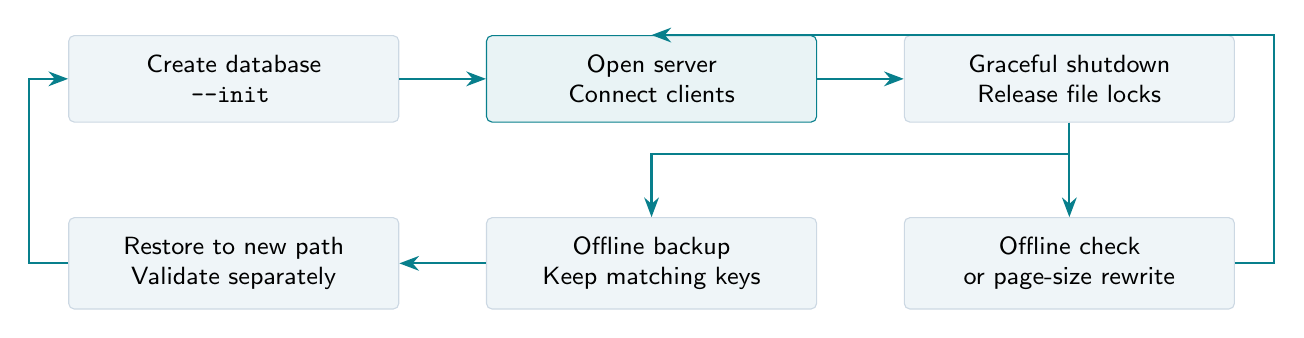
\begin{tikzpicture}[node distance=12mm and 11mm]
\node[box,text width=37mm] (init) {Create database\\\texttt{--init}};
\node[strong,text width=37mm,right=of init] (serve) {Open server\\Connect clients};
\node[box,text width=37mm,right=of serve] (stop) {Graceful shutdown\\Release file locks};
\node[box,text width=37mm,below=of init] (restore) {Restore to new path\\Validate separately};
\node[box,text width=37mm,below=of serve] (backup) {Offline backup\\Keep matching keys};
\node[box,text width=37mm,below=of stop] (check) {Offline check\\or page-size rewrite};
\draw[arrow] (init) -- (serve);\draw[arrow] (serve) -- (stop);\draw[arrow] (stop) -- (check);
\draw[arrow] (stop.south) -- ++(0,-4mm) -| (backup.north);
\draw[arrow] (backup) -- (restore);\draw[arrow] (restore.west) -- ++(-5mm,0) |- (init.west);
\draw[arrow] (check.east) -- ++(5mm,0) |- (serve.north);
\end{tikzpicture}
\caption{A safe teaching workflow. A restore is a new candidate database that must be checked before it replaces the working copy. Advanced replication has additional base, WAL and fencing requirements.}
\label{fig:database-lifecycle}
\end{figure}


\section{Create and verify a base backup}
\index{backup}

\subsection{The command-line backup is an offline operation}

The base-backup command opens the database directly and takes its normal
database ownership lock. Stop the server before invoking it. The internal
\code{runOpen} API can work with an already-open managed database, but that
does not make the public standalone CLI a network online-backup service.

Choose a destination that does not exist, including its staging counterpart:

\begin{lstlisting}
minisql-backup.exe backup C:\MiniSQL-Data\db_ACTUAL_ID `
  E:\MiniSQL-Backups\learning-base-001
\end{lstlisting}

\begin{lstlisting}[language=bash]
minisql-backup backup /srv/minisql/db_ACTUAL_ID \
  /backup/minisql/learning-base-001
\end{lstlisting}

MiniSQL captures authoritative metadata, catalog/security state, schema state,
optional statistics/encryption metadata, audit artifacts, WAL/checkpoint
state, tables, and indexes. It writes a directory containing captured files
and a checksummed \path{backup.manifest}. The report gives file count and
total bytes. The destination is not a single ZIP file and should be treated
as one complete backup unit.

Derived \path{*.heap-pages} scan directories are not needed for the backup;
restored databases rebuild them from authoritative table pages. Runtime
configuration, executable binaries, external raw keys, TLS private keys, and
ordinary server log directories are not all automatically included in this
database capture. Inventory those separately.

\subsection{Capacity and memory limitations}

The current capture code reads file images into memory and retains the
captured file collection while constructing the backup. It is not the
streaming algorithm used by the checker. A large database can therefore need
substantial working memory in addition to destination disk space. Encrypted
backup temporarily retains captured and encrypted representations as well.
Measure the largest real backup, not just a tiny demonstration database.

The explicit per-file safety limit is 4,294,967,295 bytes. The manifest uses
wide lengths, but the current implementation still applies this U32-sized
file cap. Its total safety bound is
1,152,921,504,606,846,975 bytes and its entry-count cap is U32; these format
bounds are not claims that the in-memory implementation can practically back
up that amount of data. Relative manifest paths are limited to 240 bytes and
validated against traversal/absolute-path forms.

\sourcecode{src/minisql/tools/backup.ml}{captureDatabase, runOpen, manifest limits, and path validation.}

\section{Restore a base into a new directory}
\index{restore}

\begin{lstlisting}
minisql-backup.exe restore E:\MiniSQL-Backups\learning-base-001 `
  C:\MiniSQL-Restores\learning-restore-001
minisql-check.exe C:\MiniSQL-Restores\learning-restore-001
\end{lstlisting}

The target and its \path{.restore-new} staging path must not exist. Restore
validates captured file lengths/checksums, stages the database, opens it for
recovery/verification, checks its database identity, and publishes the
validated target. It does not overwrite an existing live database in place.
The restored database retains the backup's logical database identity; the
chosen directory name is an operational path, not a new SQL database name.

After structural checking, start the restored copy on a separate unused port
and run semantic application checks: representative row counts, important
records, totals computed with the currently documented type semantics, and
relationship checks. Do not expose both the old and restored writable copy to
the same application by accident. Choose a single authoritative copy and
update application connection configuration deliberately.

If a restore fails, preserve the diagnostic and the original backup. A
leftover staging directory can be evidence of the failure. Inspect it before
removing it to retry, and never mistake a staging directory for a fully
published restore. Existing-target refusal is a deliberate guard against
overwriting prior data or a previous recovery attempt.

\sourcecode{src/minisql/tools/backup.ml}{restore and post-copy identity/consistency validation.}

\subsection{Automate the restore drill}

The repository's recovery drill performs backup, restore, and checker stages,
records timings and bounded command output, and writes a JSON report:

\begin{lstlisting}[language=bash]
python3 tools/recovery/production_recovery_drill.py \
  /srv/minisql/db_ACTUAL_ID \
  /backup/minisql/drill-base-001 \
  /srv/minisql-restores/drill-001 \
  --bin-dir build/bin-linux \
  --report build/recovery/drill-001.json
\end{lstlisting}

The default binary directory is \path{build/bin}; Linux users must select
\path{build/bin-linux} unless they have installed the programs elsewhere.
The default report path is \path{build/recovery/recovery-drill.json}.
Both output destinations must be new. This runner does not start and stop
your live server for you; arrange its offline prerequisite first.

\sourcecode{tools/recovery/production_recovery_drill.py}{Arguments, three stages, and evidence report.}

\section{Encrypt a backup independently of live TDE}

Generate a distinct 32-byte backup key outside the backup tree and create an
encrypted backup:

\begin{lstlisting}
minisqld.exe --generate-encryption-key D:\MiniSQL-Keys\backup-001.key
minisql-backup.exe backup-encrypted C:\MiniSQL-Data\db_ACTUAL_ID `
  E:\MiniSQL-Backups\learning-encrypted-001 `
  D:\MiniSQL-Keys\backup-001.key
minisql-backup.exe restore-encrypted `
  E:\MiniSQL-Backups\learning-encrypted-001 `
  C:\MiniSQL-Restores\learning-encrypted-001 `
  D:\MiniSQL-Keys\backup-001.key
\end{lstlisting}

Each captured file is encrypted/authenticated independently and remains
covered by the manifest. Wrong keys or modified encrypted payloads fail
closed. If live TDE is enabled, the backup process rewraps its DEK for the
backup provider. On restore, the same key bytes can be supplied from a new
machine-local path; MiniSQL authenticates the exported envelope and rewraps
the DEK to that restore provider identity before opening the database.

Keep the backup key available for the retained backup's lifetime. Rotating the
live KEK does not magically update already-created backups. The normal
\code{restore} command is not a substitute for \code{restore-encrypted},
and a password reset is not an encrypted-backup recovery method. The backup
key is a binary file argument, not a SQL user's password.

\sourcecode{src/minisql/tools/backup.ml}{Encrypted record format, runOpenEncrypted, and restoreEncrypted.}

\section{WAL archives and point-in-time recovery}
\index{PITR}\index{WAL archive}\index{recovery}
\begin{figure}[htbp]\centering
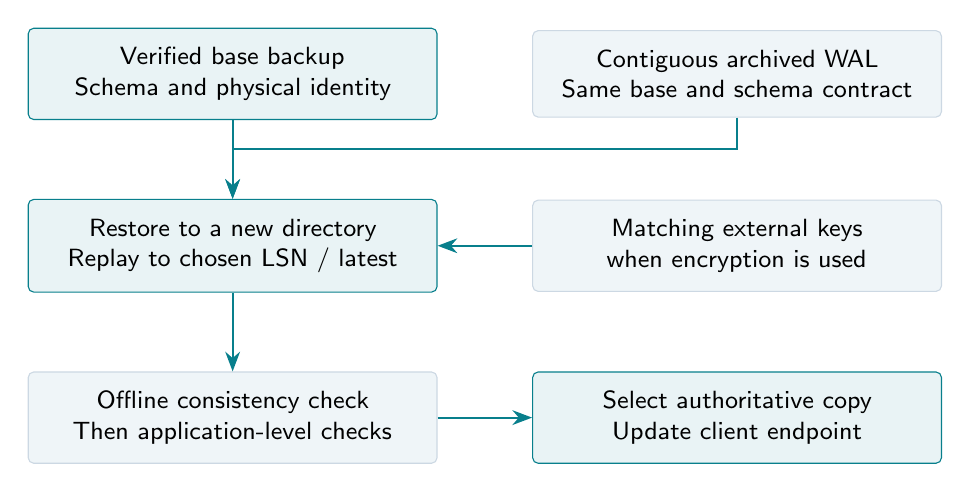
\begin{tikzpicture}[node distance=10mm and 12mm]
\node[strong,text width=47mm] (base) {Verified base backup\\Schema and physical identity};
\node[box,text width=47mm,right=of base] (wal) {Contiguous archived WAL\\Same base and schema contract};
\node[strong,text width=47mm,below=of base] (restore) {Restore to a new directory\\Replay to chosen LSN / latest};
\node[box,text width=47mm,right=of restore] (key) {Matching external keys\\when encryption is used};
\node[box,text width=47mm,below=of restore] (verify) {Offline consistency check\\Then application-level checks};
\node[strong,text width=47mm,right=of verify] (publish) {Select authoritative copy\\Update client endpoint};
\draw[arrow] (base) -- (restore);\draw[arrow] (wal.south) -- ++(0,-4mm) -| (restore.north);
\draw[arrow] (key) -- (restore);\draw[arrow] (restore) -- (verify);\draw[arrow] (verify) -- (publish);
\end{tikzpicture}
\caption{The evidence needed for point-in-time recovery. A missing WAL range, incompatible schema base or unavailable key cannot be repaired by choosing a later target.}
\label{fig:recovery-chain}
\end{figure}


\subsection{Understand the archive model}

A WAL archive contains a verified base backup and successive complete durable
WAL prefixes. Its manifest records database identity, page size, generation,
base-end LSN, latest-end LSN, WAL file name, length, and checksum. LSN is a
byte-position boundary in this WAL model, not a timestamp or SQL transaction
number.

Initialize an archive while the primary is stopped:

\begin{lstlisting}
minisql-backup.exe archive-init C:\MiniSQL-Data\db_ACTUAL_ID `
  E:\MiniSQL-Archives\learning-001
minisql-backup.exe archive-verify E:\MiniSQL-Archives\learning-001
\end{lstlisting}

Start the primary and export a durable prefix while it remains online:

\begin{lstlisting}
minisql-backup.exe archive-wal-live C:\MiniSQL-Data\db_ACTUAL_ID `
  E:\MiniSQL-Archives\learning-001
\end{lstlisting}

The live form reads the durable WAL marker and validates that the captured
prefix ends at a complete record boundary. It verifies continuity against
the previous archive prefix. If no new bytes are durable, it can return the
same generation. The \code{archive-wal} form opens the database normally
and is an offline form. Use only one archive writer for a given archive
directory.

Every generation stores a complete prefix, not only the delta from the
previous generation. Older files are retained so a verifier that already
read an older manifest can still find its referenced file. Archive growth
can therefore be substantial. Create a fresh verified base periodically and
retire old archive sets under a retention policy only after their recovery
requirements have expired.

\warning{The archive follows a fixed base schema}{The current shipping model
is intended for DML on the already archived schema/security state. After DDL,
DCL, VACUUM, page-size migration, key/envelope transitions, or operations that
rewrite or rewind physical state, stop the replication workflow and create a
new verified base. A lost WAL-prefix relationship is diagnosed; editing the
manifest does not repair it.}

\sourcecode{src/minisql/tools/backup.ml}{archiveInit, snapshotDurableWalLive, archiveWalLive, and verifyArchive.}
\sourcecode{docs/formats/wal-archive-v1.md}{Archive and standby metadata fields.}

\subsection{Automatic checkpoints can break archive continuity}

The current automatic checkpoint implementation resets the physical WAL to
zero when it reaches \code{runtime.checkpointWalBytes}, 64 MiB by default.
It has no archive-aware retention handshake. A subsequent live export then
finds that the new WAL is not an extension of the archived prefix and rejects
the export. Normal DML can reach this boundary even when no operator has
issued VACUUM or changed the schema.

Do not assume that either sidecar automatically rebases across this reset.
The hot-primary exporter propagates the failure. The HA controller's
replication error also propagates, and its cleanup stops the managed primary.
For a qualified archival workflow, plan a new base before a reset, monitor
WAL growth/checkpoint resets, and select a threshold consistent with that
maintenance window where the chosen launcher exposes configuration. The
current fenced controller uses the positional server mode and does not offer
a checkpoint-threshold argument. Increasing a threshold postpones the issue;
it does not implement archive-aware WAL retention, and the archive file-size
and memory limits still apply.

\sourcecode{src/minisql/server/database_manager.ml}{checkpointIfNeeded rewinds WAL without an archive-retention handshake.}
\sourcecode{tools/replication/minisql_ha_controller.py}{Replication failure propagation and process cleanup.}

\subsection{Restore to latest or an exact record boundary}

\begin{lstlisting}
minisql-backup.exe restore-pitr E:\MiniSQL-Archives\learning-001 `
  C:\MiniSQL-Restores\learning-latest latest
minisql-check.exe C:\MiniSQL-Restores\learning-latest
\end{lstlisting}

For an earlier recovery target, replace \code{latest} with an exact numeric
LSN taken from valid archive/WAL evidence. The target must lie between the
base-end and latest-end LSN and must be a complete record boundary. A number
in the middle of a record is rejected. There is no public
\code{restore-until-timestamp} switch; mapping a business event to an LSN
requires operational evidence outside this command.

Recovery replays committed transactions within the selected prefix. A
transaction whose commit has not been included is not made committed merely
because some of its records precede the target. When post-base authoritative
table pages have been replayed, the base indexes are marked dirty and rebuilt
before the restored generation is published. An exact base-boundary restore
can retain the already verified base indexes.

The restore destination and its \path{.pitr-stage} must be new. Preserve the
original primary if investigating an accidental change; restore separately,
check the selected state, and only then decide how to resume application
traffic. PITR is a database-wide recovery operation, not a built-in single-row
undo command.

\sourcecode{src/minisql/tools/backup.ml}{walPrefixAt, restoreToLsn, restoreLatest, and repairRecoveredIndexes.}

\section{Materialize and refresh a read-only standby}
\index{standby}

\begin{lstlisting}
minisql-backup.exe standby-materialize `
  E:\MiniSQL-Archives\learning-001 C:\MiniSQL-Standby\slot-a
minisqld.exe --serve-standby C:\MiniSQL-Standby\slot-a 7433 16
\end{lstlisting}

Materialization restores the latest verified archive state and writes a
standby marker before publishing the target. The marker records database
identity, archive generation, and applied LSN. The ordinary writable open path
rejects an unpromoted standby. The standby server permits reads and rejects
attempts to use it as a writable primary.

This describes ordinary mutation dispatch, not a complete safety guarantee for
all expression paths. In this revision, NEXTVAL can be materialized during
streaming-plan probing or EXPLAIN outside the ordinary read-only checks.
Exclude sequence-consuming expressions from standby workloads; do not use
this known gap to advance a standby's state. See the transaction and sequence
chapters for the observed behavior and restrictions.

To advance a manually managed standby, stop its server first, export the
latest primary WAL, and refresh:

\begin{lstlisting}
minisql-backup.exe standby-refresh E:\MiniSQL-Archives\learning-001 `
  C:\MiniSQL-Standby\slot-a
\end{lstlisting}

\warning{Stop the standby before refresh}{The direct refresh routine replaces
WAL/checkpoint files before opening the standby through the database manager.
Do not rely on a later lock conflict to make an attempted live refresh safe.
The public command is for a stopped standby. Use the alternating-slot sidecar
for continued read service while a separate generation is prepared.}

Refresh validates the archive identity and monotonic generation/LSN, checks
the prefix relationship, replays the new state, repairs derived indexes, and
updates the standby marker. A standby can be behind the primary even while
its server answers queries normally. Monitor applied LSN and source LSN;
availability of the read endpoint is not proof that it is current.

\sourcecode{src/minisql/tools/backup.ml}{materializeStandby, refreshStandby, and standby markers.}
\sourcecode{src/minisql/server/database_manager.ml}{Writable-open rejection of unpromoted standbys.}

\section{Continuous shipping with the hot-replica sidecar}
\index{replication}

The Python sidecar automates durable-prefix export and maintains two standby
slots. A loopback TCP switch sends new connections to the current verified
generation while another slot is prepared. Existing connections remain
associated with their selected backend; they are not silently transferred
mid-session to a different database generation. Backend retirement waits for
clients according to the sidecar's lifecycle/timeout policy.

After creating the initial archive, run the primary exporter in a separate
process:

\begin{lstlisting}[language=bash]
python3 tools/replication/minisql_hot_replica.py primary \
  --database /srv/minisql/db_ACTUAL_ID \
  --archive /srv/minisql-ha/archive \
  --backup-exe build/bin-linux/minisql-backup \
  --status-file /srv/minisql-ha/primary-status.json
\end{lstlisting}

Run the standby sidecar against that archive:

\begin{lstlisting}[language=bash]
python3 tools/replication/minisql_hot_replica.py standby \
  --archive /srv/minisql-ha/archive \
  --slot-root /srv/minisql-ha/slots \
  --backup-exe build/bin-linux/minisql-backup \
  --server-exe build/bin-linux/minisqld \
  --listen-port 7433 \
  --status-file /srv/minisql-ha/standby-status.json
\end{lstlisting}

The reference proxy binds only to loopback because it fronts a trusted
standby listener. This script does not distribute archives to another machine,
provision network storage, or add remote authentication by itself. Arrange
the intended shared/transferred archive and its access controls outside the
script. Only one process may write a particular archive.

\begin{longtable}{p{.34\linewidth}p{.59\linewidth}}
\toprule
Sidecar option & Meaning / default \\
\midrule
\endhead
Both: \code{--archive}, \code{--backup-exe} & Required archive path and
native backup executable. \\
Primary: \code{--database} & Required primary database path. \\
Both: \code{--cycles} & 0 means continue indefinitely; positive bounds are
useful for qualification. \\
Both: \code{--interval-ms} & 250 between cycles. \\
Both: \code{--command-timeout} & 600 seconds for native child operations. \\
Both: \code{--status-file}, \code{--ready-file} & Optional atomic status and
startup readiness files. \\
Standby: \code{--slot-root}, \code{--server-exe} & Required alternate-slot
root and native server executable. \\
Standby: \code{--listen-host} & \code{127.0.0.1}; loopback-only switch. \\
Standby: \code{--listen-port} & Required stable read endpoint port. \\
Standby: \code{--backend-port-a}, \code{--backend-port-b} & 0 selects free
backend ports. \\
Standby: \code{--maximum-clients} & 16 for backend native server capacity. \\
Standby: \code{--max-connections} & 0 means unlimited total proxy connections;
this is distinct from simultaneous backend capacity. \\
Standby: \code{--client-timeout} & 600 seconds in proxy/client handling. \\
\bottomrule
\end{longtable}

Use the atomic status files to monitor \code{healthy}, generation,
\code{sourceLsn}, \code{standbyLsn}, \code{lagBytes}, and
\code{cycleDurationMs}. Check both freshness and health; an old healthy file
from a stopped process is not a current success signal. The sidecar has a
\code{self-test} mode for its proxy/backend lifecycle. That test does not
replace a real database failover drill.

\sourcecode{tools/replication/minisql_hot_replica.py}{CLI, two-slot lifecycle, loopback switch, and status reports.}

\section{Promote a standby manually}

Promotion is a controlled change of authority. First stop or positively fence
the old primary so it cannot continue accepting writes. Stop the standby
server, verify the newest available archive state, and decide whether its
known replication lag is acceptable. Then run:

\begin{lstlisting}
minisql-backup.exe standby-promote C:\MiniSQL-Standby\slot-a
minisql-check.exe C:\MiniSQL-Standby\slot-a
minisqld.exe --serve C:\MiniSQL-Standby\slot-a 7432 32
\end{lstlisting}

Use the intended authenticated/TLS mode for a secured deployment instead of
the trusted demonstration mode above. Promotion publishes a promotion marker
and removes the standby marker. Recovery advances future transaction IDs
beyond observed archived transactions, avoiding reuse when the promoted
database begins writing.

Reconnect clients to the selected leader and verify one controlled write.
Existing transactions on a failed connection do not transfer to the promoted
database. Reconcile uncertain commit outcomes as described in the transaction
chapter. Rebuild the retired node from the new authoritative primary rather
than allowing both divergent copies to resume writing.

\warning{Asynchronous does not mean lossless}{A primary can acknowledge a
commit before a later shipping cycle archives it. If that primary is lost,
promotion may omit acknowledged changes that never reached the archive.
Measure and report lag; do not promise zero data loss or synchronous quorum
commit semantics.}

\sourcecode{src/minisql/tools/backup.ml}{promoteStandby.}
\sourcecode{docs/release/REPLICATION.md}{Supported failover scope and current limitations.}

\section{Automatic single-host failover and native write fencing}
\index{failover}\index{fencing}\index{HA controller}

The separate HA controller owns a local primary/backend lifecycle, a stable
loopback endpoint, a file witness, and automatic promotion. The witness
serializes leadership terms. A dedicated renewal thread updates the lease so
a long standby materialization does not by itself stop lease renewal.

The server is started with a lease path, epoch, node ID, and maximum clock
skew. It checks the persistent epoch and current lease before mutations and
again immediately before DML/DDL commit. Missing, malformed, expired, or
foreign records reject writes with error 9038. Reads and rollback remain
available for diagnosis.

\begin{lstlisting}[language=bash]
python3 tools/replication/minisql_ha_controller.py run \
  --primary-db /srv/minisql/db_ACTUAL_ID \
  --archive /srv/minisql-ha/archive \
  --slot-root /srv/minisql-ha/slots \
  --witness-dir /srv/minisql-ha/witness \
  --server-exe build/bin-linux/minisqld \
  --backup-exe build/bin-linux/minisql-backup \
  --proxy-port 7432 \
  --status-file /srv/minisql-ha/controller-status.json
\end{lstlisting}

Start this as the owner of the intended primary process; do not leave an
independently started writer running against the same directory. Use the
controller's documented disposable drill before adapting it to persistent
data. New proxy connections switch to the new leader after a promotion;
established sessions are not live-migrated and must reconnect if their backend
is retired or fails.

\begin{longtable}{p{.34\linewidth}p{.59\linewidth}}
\toprule
Controller run option & Default / meaning \\
\midrule
\endhead
\code{--primary-db}, \code{--archive}, \code{--slot-root},
\code{--witness-dir} & Required database and HA state directories. \\
\code{--server-exe}, \code{--backup-exe}, \code{--proxy-port} & Required
native executables and stable endpoint port. \\
\code{--backend-port-a}, \code{--backend-port-b} & 0 chooses free local
backend ports. \\
\code{--maximum-clients} & 32. \\
\code{--node-id} & 1; leader identity used in fencing records. \\
\code{--lease-ms} & 5000; lease duration. \\
\code{--clock-skew-ms} & 250; expiry allowance before a replacement leader
is promoted. \\
\code{--replication-ms} & 2000; replication-cycle interval. \\
\code{--command-timeout} & 300 seconds for child commands. \\
\code{--status-file} & Optional atomic controller status. \\
\code{--run-seconds} & 0 runs indefinitely. \\
\code{--max-failovers} & 0 leaves the failover count unbounded. \\
\bottomrule
\end{longtable}

The other controller modes are \code{self-test} for fencing record codecs
and \code{write-epoch --database path --epoch n --node-id n} for offline
epoch administration. They are implementation/qualification tools; changing
epochs without understanding the active lease and owner can revoke or confuse
leadership. Prefer the controller-owned workflow.

\subsection{What the witness does not provide}

A local file witness is not distributed consensus. The directory must have
one controller writer and reliable atomic-replacement semantics. Copying the
witness independently to multiple machines does not preserve one shared
leadership decision. A multiple-host design needs an external quorum-based
lease/leadership service and fencing at an authoritative write boundary.
The supplied controller does not add synchronous replication or zero-loss
commits.

The five-second lease and 250-millisecond skew allowance are operational
defaults, not universal safety guarantees for arbitrary clock behavior or
network filesystems. Qualify the actual host, process supervision, witness
filesystem, restart behavior, and client reconnection policy together.

\sourcecode{tools/replication/minisql_ha_controller.py}{Controller modes, leases, promotion, and stable endpoint.}
\sourcecode{src/minisql/server/database_manager.ml}{validateWriteFence and epoch/lease record checks.}
\sourcecode{docs/formats/ha-fencing-records-v1.md}{Persistent fencing-record formats.}

\section{Change page size with an offline rewrite}
\index{migration}\index{page size}

Changing \code{databaseDefaults.pageSize} in JSON does not rewrite a
database. The short migration command only checks whether the requested size
already matches:

\begin{lstlisting}
minisql-migrate.exe C:\MiniSQL-Data\db_ACTUAL_ID 8192
\end{lstlisting}

If the source already uses 8192, it reports success with no change. If it
uses another supported size, it reports that an offline rewrite is required
and does not modify the source. Request that rewrite explicitly:

\begin{lstlisting}
minisql-migrate.exe --rewrite C:\MiniSQL-Data\db_ACTUAL_ID `
  C:\MiniSQL-Migrated learning_8k 8192
\end{lstlisting}

The tool opens the stopped source, creates a new database under a staging
root, clones catalog/schema/security state, reads and rewrites rows at the
new page size, rebuilds indexes, checks the result, and publishes a new
UUID-based target path. It prints that actual path plus row/index counts.
The logical name is the supplied target name; the database identity is new.
The source remains available for rollback.

Supported sizes remain 4096, 8192, 16384, and 32768. Current copy code
materializes each source table's rows for rewriting, so plan memory as well
as additional disk capacity. It preserves the supported schema extensions,
including views, sequences, triggers, and procedure definitions, through the
cloned schema state, but it does not copy the old physical WAL history or
automatically preserve the source's TDE envelope. Enable/verify encryption
on the new target if required, refresh optimizer statistics as appropriate,
and create a fresh replication base.

This command accepts only databases the current engine can open. It cannot
convert a rejected format-1 database into format 2. For that version boundary,
use the old matching engine to extract logical data and rebuild it in a new
current-format database. Compare actual rows and schema objects before
retiring the old copy.

\sourcecode{src/minisql/tools/migrate.ml}{plan, run, copyDatabaseState, and rewrite.}
\sourcecode{src/apps/minisql_migrate/main.ml}{Public migration arguments and success output.}

\section{Complete backup, checker, and migration command reference}

\begin{lstlisting}
minisql-check --version
minisql-check --m0-self-test
minisql-check <database>

minisql-backup --version
minisql-backup --m0-self-test
minisql-backup backup <database> <new-backup>
minisql-backup backup-encrypted <database> <new-backup> <key-file>
minisql-backup restore <backup> <new-database>
minisql-backup restore-encrypted <backup> <new-database> <key-file>
minisql-backup archive-init <database> <new-archive>
minisql-backup archive-wal <stopped-database> <archive>
minisql-backup archive-wal-live <database> <archive>
minisql-backup archive-verify <archive>
minisql-backup restore-pitr <archive> <new-database> <lsn|latest>
minisql-backup standby-materialize <archive> <new-standby>
minisql-backup standby-refresh <archive> <stopped-standby>
minisql-backup standby-promote <stopped-standby>

minisql-migrate --version
minisql-migrate --m0-self-test
minisql-migrate <stopped-database> <page-size>
minisql-migrate --rewrite <stopped-source> <target-root>
  <target-name> <page-size>
\end{lstlisting}

Use \path{.exe} on Windows. The bracketed \code{lsn|latest} position means
choose a numeric LSN or the literal \code{latest}; do not pass the bar.
Wrapped reference lines are one command. These tools return 0 on success,
1 for a reported operational failure, and 2 for invalid usage. Preserve the
printed error code/message, rather than treating every nonzero exit as a
generic copy failure.

\sourcecode{src/apps/minisql_backup/main.ml}{Complete backup/archive/standby dispatch.}
\sourcecode{src/apps/minisql_check/main.ml}{Checker dispatch and warnings.}
\sourcecode{src/apps/minisql_migrate/main.ml}{Migration dispatch.}

\section{A recovery rehearsal from beginning to end}

For a disposable learning database, insert a distinctive baseline record,
stop the server, and create a base/archive. Restart it, insert a second record,
and export a live WAL prefix. Restore the base to one fresh path and the
latest archive to another. Verify that the base has only the baseline record
and the latest restore includes the later committed record. Run the checker
on each stopped copy.

Next materialize a standby, query it through a standby listener, and confirm
that a write is rejected. Stop the original primary and standby listener,
promote the standby, restart it in the intended writable mode, and commit a
third record. This teaches the distinction between a verified backup, an
applied archive generation, a read-only standby, and an authoritative writable
leader.

For automated qualification, use the repository's production failover,
automatic-fencing, and automatic-controller drills in new empty work roots.
The fencing drill deliberately leaves an old leader alive and verifies write
rejection; the controller drill terminates a controller-owned leader and
checks promotion. Keep the reports, repeat them for the deployed revision,
and measure recovery time on data volumes representative of the actual
installation.

\sourcecode{tests/ha/production_failover_drill.py}{Live shipping and manual promotion drill.}
\sourcecode{tests/ha/automatic_fencing_drill.py}{Stale-writer rejection and fenced leadership transition.}
\sourcecode{tests/ha/automatic_controller_live.py}{Controller-owned leader failure and automatic promotion.}

\part{Build, Diagnose and Understand}
\chapter{Clients, Workbench, and Application Integration}
\label{adv:clients}

\section{Choose the interface for the task}

A MiniSQL server process exposes one database at one endpoint. A client connects to that endpoint; it does not select an unrelated database with a \code{USE} statement. Database names in a Python DSN, JDBC URL, or Workbench alias are labels. To use a second database, start or connect to its server endpoint. This distinction explains why changing a catalog label does not change the data you see.

\begin{longtable}{p{.23\linewidth}p{.68\linewidth}}
\toprule Interface & Appropriate use \\\midrule
Native console & Interactive SQL, small UTF-8 scripts, connectivity checks, and operator workflows on Windows or Linux. \\
Windows Workbench & Exploring objects, editing worksheets, inspecting results, staged data editing, and schema design. \\
Python connector & Import/export programs, repeatable analysis, teaching examples, and application services. Python 3.10 or newer is required. \\
JDBC driver & Java applications and tools that accept a JDBC driver. Java 11 or newer is required. \\
MiniLang modules & In-process use of the same engine or native client facilities. This is a source integration, not a separately versioned C ABI. \\
\bottomrule
\end{longtable}

Every interface ultimately uses the same SQL engine, but their transaction defaults and result representations differ. Learn the connector's behavior before moving a script from the shell into an application.
\sourcecode{src/apps/minisql/main.ml}{Native client entry points.}
\sourcecode{clients/python/minisql/dbapi.py}{Python connection and transaction behavior.}
\sourcecode{clients/jdbc/src/main/java/org/minilang/minisql/jdbc/MiniSqlJdbc.java}{JDBC connection and statement handlers.}

\section{The native console}
\index{console}\index{shell}\index{scripts}
\subsection{Connect, query, or run a script}

The executable is \path{build/bin/minisql.exe} on Windows and \path{build/bin-linux/minisql} on Linux. The examples below use the Linux name; use the Windows executable path in PowerShell. Native client commands return exit status 0 on success, 1 for operational or SQL failure, and 2 for invalid command-line usage.

\begin{lstlisting}[language=bash]
./build/bin-linux/minisql --ping 7432
./build/bin-linux/minisql --query 7432 "SHOW TABLES;"
./build/bin-linux/minisql --shell 7432
./build/bin-linux/minisql --script 7432 docs/manual/examples/01-create-shop.sql
\end{lstlisting}

The trusted forms connect to loopback. A successful ping prints \code{PONG}. Query mode formats the request's ordered results and closes its connection; separate query invocations therefore do not share a transaction, prepared statement, or session state. Shell mode and script mode keep a connection open across their statements.

The complete connection families are listed below. Replace \code{ACTION} with \code{ping}, \code{query}, \code{shell}, or \code{script}. Query takes an additional SQL argument; script takes an additional filename. Ping and shell have no trailing argument.

\begin{longtable}{p{.25\linewidth}p{.66\linewidth}}
\toprule Family & Argument order after the executable \\\midrule
Trusted loopback & \path{--ACTION <port> [sql-or-file]} \\
Password prompt, loopback & \path{--auth-ACTION-prompt <port> <user> [sql-or-file]} \\
Password-authenticated protected framing & \path{--secure-ACTION <address> <port> <user> [sql-or-file]} \\
Native TLS & \path{--tls-ACTION <address> <port> <server-name> <user> [sql-or-file]} \\
Native TLS with leaf pin & \path{--tls-pin-ACTION <address> <port> <server-name> <sha256-pin> <user> [sql-or-file]} \\
Version & \path{--version} \\
\bottomrule
\end{longtable}

\begin{lstlisting}[language=bash]
./build/bin-linux/minisql --auth-shell-prompt 7432 analyst
./build/bin-linux/minisql --tls-shell \
  db.example.test 7443 db.example.test analyst
\end{lstlisting}

The authenticated modes prompt for the password. All authenticated connections enable MiniSQL protected framing after authentication, including authenticated loopback and TLS-wrapped sessions. The \code{secure} family is MiniSQL's authenticated encrypted framing; the \code{tls} family explicitly negotiates native TLS. These names are not interchangeable. The client and listener must agree on the transport. A SHA-256 pin in the native client identifies the exact DER leaf certificate; obtain it through a trusted administrative channel.

\subsection{Work efficiently in the shell}

Statements may span lines. The prompt changes from \code{minisql>} to \code{...>} while an unfinished SQL fragment is buffered. The default terminator is a semicolon outside a string, quoted identifier, or comment. Use \code{DELIMITER \$\$} before a compound procedure definition, end the definition with \code{\$\$}, and restore \code{DELIMITER ;} afterward. The delimiter is connection-local client input state and is never sent as SQL. Backslash commands are also client commands.

\begin{longtable}{p{.28\linewidth}p{.63\linewidth}}
\toprule Command & Effect \\\midrule
\path{\help} & Display the shell command list. \\
\path{\q}, \path{\quit} & Close the session when no SQL fragment is pending. \\
\path{\g} & Execute the current multiline buffer without requiring a final semicolon. \\
\path{\reset} & Discard the current unfinished buffer. \\
\path{\source <file>} & Run a UTF-8 SQL script in the same session. \\
\path{\tables} & Execute \code{SHOW TABLES}. \\
\path{\describe <table>} & Execute \code{DESCRIBE table}. \\
\path{\indexes <table>} & Execute \code{SHOW INDEXES FROM table}. \\
\path{\ping} & Perform a protocol liveness check. \\
\bottomrule
\end{longtable}

Use SQL directly for names that need quoting rather than relying on the restricted identifier parser in a metadata shortcut. Most backslash commands are recognized only when the SQL buffer is empty. If a forgotten quote or incomplete statement prevents \path{\q} from behaving as expected, enter \path{\reset} first.

\begin{lstlisting}[language=SQL]
SELECT customer_id, name
FROM customers
WHERE active = TRUE
ORDER BY customer_id;
\end{lstlisting}

\subsection{Script semantics and limits}

A script is scanned with the same quote-aware and comment-aware logic as interactive input. The final SQL statement need not end with a semicolon. Statements execute in order, and processing stops at the first error. Success prints \code{MiniSQL script completed statements=N}. The script reader currently accepts at most 1 MiB of file content; this limit is separate from the protocol's larger frame limit. Split large imports into smaller scripts or use connector batches.

Running a script does not make its statements one transaction. Add \code{BEGIN} and \code{COMMIT} around related DML when atomicity is required. Keep schema changes separate from the DML transaction, and understand what already committed before retrying a partly completed script. A script contains SQL and optional \code{DELIMITER} directives; \path{\source} remains an interactive shell command rather than an SQL include directive.

\sourcecode{src/minisql/client/console.ml}{scanSqlBatch, executeStatements, runScript, printShellHelp, and runShell.}

\section{The Windows Workbench}
\index{Workbench}\index{GUI}
\begin{figure}[htbp]\centering
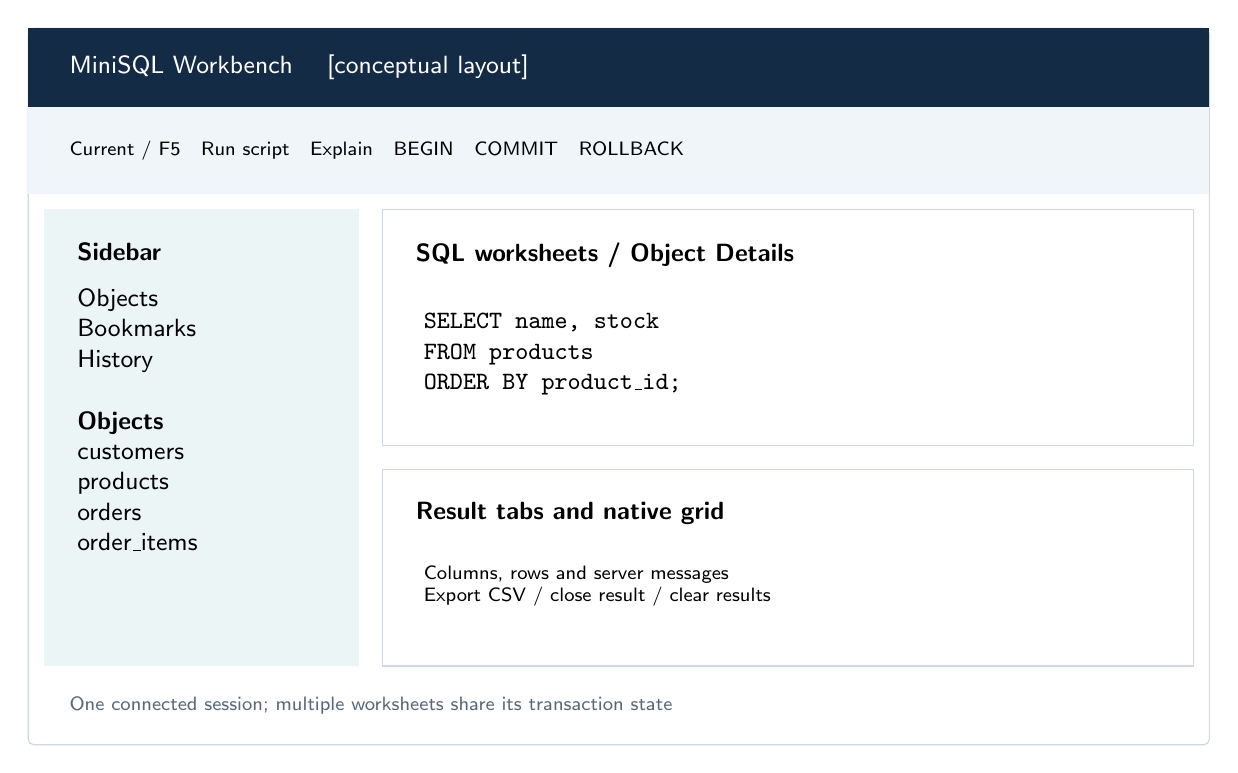
\begin{tikzpicture}[x=1mm,y=1mm]
\draw[draw=Rule,fill=white,rounded corners=2pt] (0,0) rectangle (150,91);
\fill[Navy] (0,81) rectangle (150,91);
\node[font=\sffamily\small,text=white,anchor=west] at (4,86) {MiniSQL Workbench \quad [conceptual layout]};
\fill[Pale] (0,70) rectangle (150,81);
\node[font=\sffamily\scriptsize,anchor=west] at (4,75.5) {Current / F5\quad Run script\quad Explain\quad BEGIN\quad COMMIT\quad ROLLBACK};
\fill[Teal!8] (2,10) rectangle (42,68);
\node[font=\sffamily\small,align=left,anchor=north west,text width=35mm] at (5,65) {\textbf{Sidebar}\\[2mm]Objects\\Bookmarks\\History\\[4mm]\textbf{Objects}\\customers\\products\\orders\\order\_items};
\draw[Rule] (45,38) rectangle (148,68);
\node[font=\sffamily\small,anchor=north west] at (48,65) {\textbf{SQL worksheets / Object Details}};
\node[font=\ttfamily\small,align=left,anchor=north west] at (49,56) {SELECT name, stock\\FROM products\\ORDER BY product\_id;};
\draw[Rule] (45,10) rectangle (148,35);
\node[font=\sffamily\small,anchor=north west] at (48,32) {\textbf{Result tabs and native grid}};
\node[font=\sffamily\scriptsize,align=left,anchor=north west] at (49,24) {Columns, rows and server messages\\Export CSV / close result / clear results};
\node[smalllabel,anchor=west] at (4,5) {One connected session; multiple worksheets share its transaction state};
\end{tikzpicture}
\caption{A navigation map of Workbench concepts. This is an explanatory drawing, not a screenshot or a pixel-exact representation of the Windows interface.}
\label{fig:workbench-map}
\end{figure}

\subsection{Create a connection alias}

Launch \path{build/bin/minisql-admin.exe}. The first-run \emph{Local MiniSQL} alias points to trusted loopback on port 7432. Use trusted local mode only with a matching trusted listener. To connect to an authenticated listener, clear trusted mode, enter the endpoint and user, and provide the password when connecting. For TLS, enable \emph{Native TLS 1.3 / X.509}, enter the expected certificate name, and optionally enter the leaf fingerprint.

Aliases store endpoint, database label, username, transport settings, and optional pin. They do not store passwords. The normal location is \path{%APPDATA%/MiniSQL/workbench-profiles.json}; \code{MINISQL\_ADMIN\_PROFILE\_PATH} overrides it. The adjacent persisted window state restores a valid previous position and size. A failed connection displays an actionable dialog and returns to the connection manager so settings can be corrected.

\begin{lstlisting}
build\bin\minisql-admin.exe --connect-local 7432 shop
build\bin\minisql-admin.exe --connect 127.0.0.1 7432 analyst shop
build\bin\minisql-admin.exe --connect-tls db.example.test 7443 db.example.test analyst shop
\end{lstlisting}

The TLS shortcut accepts an optional SHA-256 pin after the database label. Do not include a password in a shortcut or alias file.

\subsection{Understand the workspace}

The sidebar contains \emph{Objects}, \emph{Bookmarks}, and \emph{History}. The object tree comes from the connected database's metadata. Bookmarks insert useful SQL templates. History retains the newest 100 worksheet batches and provides a search filter. Account statements containing passwords are redacted from history and worksheet/result state.

The main workspace contains SQL worksheets and object-detail pages. Each worksheet has independent text. Results are kept in bounded tabs, with up to 32 recent result tabs. The result view includes column headers, rows, elapsed time, success status, and server messages. Closing a result tab affects that result only. \emph{Clear results} removes all result tabs.

\begin{longtable}{p{.3\linewidth}p{.61\linewidth}}
\toprule Action & Meaning \\\midrule
Current / F5 & Run the selection, or the statement containing the caret when nothing is selected. \\
Run script / \mbox{Ctrl+}\allowbreak\mbox{Shift+Enter} & Run all statements in the worksheet in source order. \\
Explain & Explain exactly one statement in the current/selection scope. \\
+ SQL / Ctrl+N & Create a worksheet. \\
Close SQL / Ctrl+W & Close a worksheet; nonempty text requires confirmation. A fresh blank worksheet replaces the last closed one. \\
Export CSV / Ctrl+E & Save the active result with CSV quote escaping. \\
BEGIN, COMMIT, ROLLBACK & Send the corresponding SQL transaction command. \\
Stop & Stop the active worker and disconnect this session. Reconnect before further work. \\
\bottomrule
\end{longtable}

The application uses a background native worker for execution and metadata loading. Controls that would concurrently access session state are disabled until the worker publishes its result. A responsive window is not evidence that the database statement has completed: check the status and result tab.

Workbench scripts also recognize \code{DELIMITER}. Procedure result sets retain
separate result boundaries, even when successive SELECT statements have the same
column names.

\warning{Workbench Stop is a disconnect}{The current Workbench does not use the newer cooperative cancellation facility exposed by Python and JDBC. Its Stop path aborts the connection to avoid reusing an interrupted response stream. Any uncommitted work needs to be assessed after reconnection. Do not interpret Stop as confirmation that a previously acknowledged commit was undone.}

\subsection{Inspect and edit table data}

Select a table and choose \emph{Open object}. The detail pages show Summary, Columns, Indexes, Data, Row Count, and reconstructed DDL. The Data page normally loads 100 rows per page; the underlying browse API permits page sizes from 1 to 1000. Column headers toggle sorting. The filter accepts one \code{WHERE} predicate and rejects statement terminators or comment openers.

\emph{Add row}, \emph{Copy row}, and \emph{Edit row} open a field editor. A double-click starts editing at the selected cell. Use \code{<NULL>} for SQL NULL. Insert fields can use \code{<DEFAULT>} for defaults or identity values. Text is escaped as SQL; numeric and Boolean inputs are checked before staging.

Edits are staged locally. This gives a deliberate review sequence:

\begin{enumerate}
\item Browse and filter to the intended rows.
\item Stage inserts, updates, or deletions. Pending rows are visibly marked.
\item Inspect \emph{SQL preview}; this is the exact SQL the Workbench plans to send.
\item Choose \emph{Apply changes} to execute the batch, or \emph{Revert} to discard local changes.
\end{enumerate}

Apply uses a transaction, or a savepoint when appropriate, and rolls the batch back on failure. Updates and deletes require a usable primary key or unique index so that a generated predicate can identify one row. If the table lacks such a key, define one with a meaningful business invariant or use an explicitly reviewed SQL statement. While edits are pending, paging, filtering, and sorting are disabled to keep staged row identities stable.

Copy places a header and selected rows on the clipboard as escaped tab-separated Unicode text. Paste requires a matching header and stages at most 1000 inserts. This is useful for controlled small edits; connector imports are better for larger data sets and explicit type conversion.

\subsection{Use the schema designer}

\emph{Schema} supports create/drop/rename table, add/drop/rename column, create/drop index, and add/drop constraint operations. It quotes identifier components, validates definition fields, and displays either generated DDL or a validation error. \emph{Insert into SQL} opens the generated statement in a new worksheet without executing it. \emph{Execute DDL} asks for explicit confirmation, executes the statement, and refreshes metadata after success.

The designer cannot make an engine restriction disappear. For example, a requested column drop can still be rejected because data or dependencies make it unsupported. Read the exact DDL and engine diagnostic. The reconstructed DDL page is useful for understanding an object; use the documented backup tools for a restorable physical database copy.

\sourcecode{src/minisql/admin/fullclient.ml}{Profiles, result/history bounds, browse/edit SQL generation, staged batches, and schema designer.}
\sourcecode{src/minisql/admin/win32_client.ml}{Native controls, execution workers, keyboard actions, and Stop behavior.}
\sourcecode{src/apps/minisql_admin/main.ml}{Workbench command-line dispatch.}

\section{Python DB-API integration}
\index{Python}\index{DB-API}
\subsection{Install and open a connection}

Install the source package from the repository root:

\begin{lstlisting}[language=bash]
python -m pip install ./clients/python
\end{lstlisting}

The distribution name is \code{minisql-connector}, while the import name is \code{minisql}. The package declares \code{cryptography>=41}; password authentication uses it for authenticated encryption. TLS uses Python's \code{ssl} module. The module reports \code{apilevel='2.0'}, \code{paramstyle='qmark'}, and \code{threadsafety=1}: threads can share the module, but should use separate connections.

\begin{lstlisting}[language=Python]
import minisql

connection = minisql.connect(
    host="127.0.0.1", port=7432, database="shop"
)
try:
    with connection:
        with connection.cursor() as cursor:
            cursor.execute(
                "SELECT customer_id, name FROM customers "
                "WHERE active = ? ORDER BY customer_id",
                (True,),
            )
            for customer_id, name in cursor:
                print(int(customer_id), name)
finally:
    connection.close()
\end{lstlisting}

The explicit \code{int} conversion is intentional: ordinary network results contain strings or \code{None}, not automatically typed Python numbers. The connection context manager commits on normal exit and rolls back if an exception escapes. It does \emph{not} close the connection. A cursor context manager does close its cursor.

\subsection{Connection options}

\begin{longtable}{p{.28\linewidth}p{.63\linewidth}}
\toprule Keyword & Default and meaning \\\midrule
\code{host}, \code{port} & \code{127.0.0.1}, 7432. Port must be 1--65535. \\
\code{database} & \code{main}; a nonempty client label, not a server-side database switch. \\
\code{user}, \code{password} & No user selects trusted mode; password defaults to empty. Supply actual credentials for authenticated listeners. \\
\code{tls} & \code{False}; enable TLS 1.3. \\
\code{server\_name} & Host; certificate name and TLS SNI name. \\
\code{pin\_sha256} & None; exactly 32 bytes written as 64 hexadecimal digits. Colons and hyphens may separate digits. \\
\code{trust\_\allowbreak server\_\allowbreak certificate} & \code{False}; pin-only trust. Requires a valid pin and TLS. \\
\code{ca\_file} & None; private CA bundle for ordinary certificate validation. Requires TLS. \\
\code{connect\_timeout} & 10 seconds; 0--3600, with 0 selecting blocking I/O. \\
\code{socket\_timeout} & 30 seconds; 0--3600, with 0 selecting blocking I/O. \\
\code{autocommit} & \code{False}; lazy explicit transactions are the default. \\
\code{isolation\_level} & \code{SERIALIZABLE}; also accepts \code{READ COMMITTED}. \\
\bottomrule
\end{longtable}

The DSN form is \path{minisql://host:port/database}. It can contain URL-encoded user/password information and the supported query options, but keyword credentials are easier to keep out of logs. Non-\code{None} keyword arguments override DSN values. Unknown DSN options are rejected.

\begin{lstlisting}[language=Python]
import os
import minisql

connection = minisql.connect(
    "minisql://db.example.test:7443/shop",
    user="application",
    password=os.environ["MINISQL_PASSWORD"],
    tls=True,
    server_name="db.example.test",
    ca_file="deployment-ca.pem",
)
\end{lstlisting}

Normal TLS validates the trust chain and hostname; an optional pin adds an exact leaf check. Pin-only trust is different: \code{trust\_server\_certificate=True} disables Python's ordinary chain and hostname validation and relies on the supplied exact leaf digest, TLS 1.3, and the required cipher. It must be an intentional deployment choice. Native Workbench pinning has a stricter validation policy; do not assume the two implementations have identical certificate checks. Python's pin option accepts hexadecimal digits with separators, not the native client's \code{sha256:} prefix.

\subsection{Parameters and values}

Use \code{?} placeholders for values. They cannot stand for table names, column names, or SQL keywords. The scanner ignores markers inside strings, quoted identifiers, and comments. Parameter counts must match. Do not build SQL by concatenating user-supplied values.

\begin{lstlisting}[language=Python]
from decimal import Decimal

with connection.cursor() as cursor:
    cursor.execute(
        "INSERT INTO products(product_id,name,price,stock) "
        "VALUES (?,?,?,?)",
        (106, "Field notebook", Decimal("12.50"), 20),
    )
connection.commit()
\end{lstlisting}

\begin{longtable}{p{.29\linewidth}p{.62\linewidth}}
\toprule Python value & Binding behavior \\\midrule
\code{None} & SQL NULL. \\
\code{bool} & TRUE or FALSE. \\
\code{int} & Decimal integer text, checked against the destination SQL type by the server. \\
\code{float}, \code{Decimal} & Finite numeric text. Non-finite values are rejected. Use Decimal for exact business quantities. \\
\code{str} & A quoted SQL string with embedded apostrophes doubled. \\
\code{datetime.date} & Epoch-day integer cast to DATE. \\
\code{datetime.time} & Microseconds since midnight cast to TIME; timezone-aware values are rejected. \\
\code{datetime.datetime} & Epoch microseconds cast to TIMESTAMP; timezone-aware values are rejected. \\
\code{bytes}, \code{bytearray}, \code{memoryview} & Binding is unsupported because SQL has no binary literal. \\
\bottomrule
\end{longtable}

The module also supplies \code{Date}, \code{Time}, \code{Timestamp}, their \code{FromTicks} constructors, and \code{Binary}. The latter creates a Python byte object; it does not add a binary transport-binding capability.

Parameterized SELECT, INSERT, UPDATE, DELETE and CALL statements use a
session-local LRU cache of at most 128 server PREPARE plans. Other accepted
statement forms use validated literal substitution. There is no typed binary
parameter frame. Cache reuse saves preparation work but does not justify
sharing one connection among simultaneous workers.

\subsection{Transactions and DDL boundaries}

With the default autocommit setting, the first non-DDL operation lazily sends \code{BEGIN ISOLATION LEVEL SERIALIZABLE READ WRITE}. \code{commit()} or \code{rollback()} finishes the active transaction; each is a no-op when idle. Setting \code{autocommit=True} commits an active transaction. Change \code{isolation\_level} only between transactions.

The connector treats CREATE, ALTER, DROP, TRUNCATE, VACUUM, REINDEX, and ANALYZE specially: it commits an active DB-API transaction immediately before sending the operation implicitly. Thus schema or maintenance work inside a Python \code{with connection:} block can commit earlier DML. Keep schema installation and business transactions separate.

\begin{lstlisting}[language=Python]
try:
    with connection.cursor() as cursor:
        cursor.execute(
            "UPDATE products SET stock=stock-? "
            "WHERE product_id=? AND stock>=?", (2, 101, 2)
        )
        if cursor.rowcount != 1:
            raise ValueError("Product absent or insufficient stock")
    connection.commit()
except Exception:
    connection.rollback()
    raise
\end{lstlisting}

Avoid manually sending BEGIN/COMMIT while also relying on the connector's transaction tracking. For an administrative SQL script requiring direct session control, use autocommit mode and deliberately manage all SQL boundaries yourself.

\subsection{Cursor API and streaming}

\begin{longtable}{p{.29\linewidth}p{.62\linewidth}}
\toprule Member & Current behavior \\\midrule
\code{execute(sql, parameters)} & Execute one operation and return the cursor. \\
\code{executemany(sql, iterable)} & Consume parameter sets incrementally; optimize compatible inserts into bounded multirow requests. \\
\code{fetchone()} & Return one tuple, or None after exhaustion. \\
\code{fetchmany(size)} & Return up to the requested rows; uses \code{arraysize} if omitted. \\
\code{fetchall()} & Materialize all remaining rows in a list. \\
Iteration & Advance through the result stream until exhausted. \\
\code{description} & Seven-field DB-API column descriptions; negotiated result type families when available, generic STRING otherwise. None for commands. \\
\code{rowcount} & Affected rows for a command; -1 for a SELECT result. \\
\code{lastrowid} & None. Use SQL RETURNING when an inserted identifier is required. \\
\code{setinputsizes}, \code{setoutputsize} & Accepted as no-op hints. \\
\code{callproc(name, parameters)} & Return IN values and updated OUT/INOUT values as a tuple; spool result frames to a temporary file for subsequent fetching. \\
\code{nextset()} & Discard unread rows of the current result and advance; return None when no further result exists. \\
\code{close()} & Drain every remaining result and release the cursor. \\
\bottomrule
\end{longtable}

Only one unread result stream may own a connection. Consume or close it before another operation. Closing a cursor can involve network reads because pending frames must be drained. Fetching in chunks bounds application-held rows; \code{fetchall()} removes that benefit. Server operators may still materialize intermediate or final results, so a streaming client is not proof that the entire query uses constant memory.

\begin{lstlisting}[language=Python]
with connection.cursor() as cursor:
    cursor.execute("SELECT product_id,name,price FROM products ORDER BY product_id")
    while True:
        batch = cursor.fetchmany(200)
        if not batch:
            break
        for identifier, name, price in batch:
            process_product(int(identifier), name, Decimal(price).scaleb(-2))
\end{lstlisting}

Here \code{process\_product} is an application function supplied by the reader, not a connector API. The \code{scaleb(-2)} conversion is required for the known \code{DECIMAL(10,2)} column: this implementation returns its scaled integer coefficient as text. For example, a stored 12.50 is returned as \code{1250}. Do not apply this conversion blindly to arbitrary expressions or columns with another scale.

\subsection{Stored procedure calls}

For the \code{sum\_to} procedure defined in Chapter~8, supply a placeholder for
its OUT argument. The original Python IN value is preserved. With a current
server, negotiated OUT and INOUT values retain their SQL type:

\begin{lstlisting}[language=Python]
with connection.cursor() as cursor:
    returned = cursor.callproc("sum_to", (5, None))
    assert returned == (5, 15)
\end{lstlisting}

\code{callproc} drains the call before returning its outputs and spools result
frames, spilling to a private temporary file after 1 MiB. Fetching then replays
the stored frames with bounded memory; closing the cursor releases them.
This avoids retaining every row in RAM,
but still requires disk space and waits for the complete call. For immediate
incremental consumption, use \code{execute("CALL ...")}, consume the current
result when \code{description} is not None, and repeat with \code{nextset()}.
Distinct SELECTs remain distinct even when their columns match. A later error
in this streaming form is raised when advancing to its result boundary.

Typed outputs include Boolean, integer, float, Decimal, text, bytes, date,
time and datetime values; SQL NULL becomes None while literal text NULL stays
text. An older server without the negotiated extension retains text/None output
values, so the example's OUT value would be \code{"15"} in that fallback mode.
Quoted and schema-qualified procedure identifiers are accepted.
When using explicit output session variables, query them after consuming every
CALL result. Submit complete compound CREATE definitions to \code{execute};
the client-only \code{DELIMITER} directive is omitted from API SQL strings.

\subsection{Import and export data}
\index{CSV}\index{import}\index{export}

There is no SQL \code{COPY} or \code{LOAD DATA} command in this implementation. Use a connector to parse an interchange file, validate its values, and bind them. A CSV import can remain incremental:

\begin{lstlisting}[language=Python]
import csv
from decimal import Decimal

with open("products.csv", newline="", encoding="utf-8") as source:
    records = csv.DictReader(source)
    parameters = (
        (int(row["product_id"]), row["name"],
         Decimal(row["price"]), int(row["stock"]))
        for row in records
    )
    try:
        with connection.cursor() as cursor:
            cursor.executemany(
                "INSERT INTO products(product_id,name,price,stock) "
                "VALUES (?,?,?,?)", parameters
            )
        connection.commit()
    except Exception:
        connection.rollback()
        raise
\end{lstlisting}

Compatible single-row INSERT operations are grouped into requests of at most 256 rows and 768 KiB of SQL. If a grouped request fails, the connector retries original entries in order; a savepoint protects an explicit transaction before this fallback. This preserves first-failure behavior, not an automatic all-file rollback. The surrounding exception handler above makes the import atomic by rolling back the whole explicit transaction. With autocommit enabled, earlier successful entries can remain committed.

For export, use \code{csv.writer}, write headers from \code{cursor.description},
and iterate through the cursor. Choose and document a NULL convention in the
output file. Current peers negotiate an exact per-cell NULL bitmap; older
peers using the legacy result format still conflate SQL NULL and literal text
\code{NULL}. Account for the negotiated format before promising exact export
round-tripping.

\subsection{Errors and cancellation}

Negotiated errors expose \code{code}, \code{sqlstate} and the message without
requiring message parsing. SQLSTATE class 23 maps to \code{IntegrityError},
22 to \code{DataError}, 42 to \code{ProgrammingError}, and 0A to
\code{NotSupportedError}; connection and transaction-retry classes use
\code{OperationalError}. Other states may use the base \code{DatabaseError}.
For legacy peers the connector retains its native-code fallback, including
constraint errors 9021/9022 and type mismatch 9017. Do not rely on every
operational failure having the same Python subclass.

\code{cursor.messages} and \code{connection.messages} expose the DB-API warning
extension as pairs of Warning class and Warning instance. Each warning retains
its SQLSTATE, code and message. Cursor warnings remain associated with that
cursor even if another statement is subsequently executed on the connection.

\code{Connection.cancel()} opens a short-lived control connection using the same connection settings and targets the session identifier learned during HELLO. It is designed to work while the query connection is blocked. Trusted-local callers can use it directly; authenticated callers need database ADMIN. Alternatively, a separate administrator connection can call \code{cancel\_session(id)} for a session shown by SHOW PROCESSLIST. Cancellation is cooperative: success means the token was set; the target observes it at a polling boundary and reports error 9035. Handle any resulting transaction failure and roll back as required before reusing it.

\sourcecode{clients/python/minisql/dbapi.py}{Complete public connection/cursor API, binding, batches, and DDL classification.}
\sourcecode{clients/python/minisql/protocol.py}{TLS policy, continuation frames, cancellation, and server-error mapping.}

\section{Java and JDBC integration}
\index{Java}\index{JDBC}
\subsection{Build and connect}

Build from the repository root with \path{clients/jdbc/build.ps1}; the JAR is \path{build/jdbc/minisql-jdbc-1.1.1.jar}. Alternatively run \code{mvn package} in \path{clients/jdbc}. The driver has no runtime dependencies and includes the JDBC service registration. With the JAR on the classpath, \code{DriverManager} finds \code{org.minilang.minisql.jdbc.MiniSqlDriver}; explicit \code{Class.forName} is optional for older frameworks.

\begin{lstlisting}[language=Java]
import java.sql.*;

try (Connection connection = DriverManager.getConnection(
        "jdbc:minisql://127.0.0.1:7432/shop")) {
    try (PreparedStatement statement = connection.prepareStatement(
            "SELECT product_id,name,price FROM products " +
            "WHERE stock >= ? ORDER BY product_id")) {
        statement.setInt(1, 1);
        try (ResultSet rows = statement.executeQuery()) {
            while (rows.next()) {
                System.out.println(rows.getInt("product_id") + " " +
                    rows.getString("name") + " " +
                    rows.getBigDecimal("price").movePointLeft(2));
            }
        }
    }
}
\end{lstlisting}

A URL has the form \path{jdbc:minisql://host[:port]/database[?property=value&...]}. It labels the endpoint's catalog; \code{setCatalog} refuses a different catalog. Schemas still use explicit two-part SQL names; the driver's \code{setSchema} accepts only public and does not establish a search path.

\begin{longtable}{p{.3\linewidth}p{.61\linewidth}}
\toprule Property & Default and use \\\midrule
\code{user}, \code{password} & No user means trusted mode; prefer a Properties object for credentials. \\
\code{tls} & false; enable TLS 1.3 with the required AES-256-GCM suite. \\
\code{serverName} & URL host; SNI and ordinary endpoint validation name. \\
\code{pinSha256} & None; 64 hexadecimal digits, optionally separated with colons or hyphens. \\
\code{trustServerCertificate} & false; pin-only trust, requiring a valid leaf pin. \\
\code{connectTimeoutMs} & 10000; TCP connection timeout, zero for platform default. \\
\code{socketTimeoutMs} & 30000; socket read timeout, zero disables it. \\
\bottomrule
\end{longtable}

URL query properties override values from the Properties object, unlike Python's keyword-over-DSN rule. Ordinary TLS validates the chain through the JVM trust store and performs endpoint-name validation. Adding a pin also checks the exact leaf digest. Pin-only mode disables ordinary trust and endpoint-name checks and relies on the exact pinned leaf; provision and rotate that pin deliberately.

\subsection{Transaction behavior}

JDBC defaults to autocommit true. To start a business transaction, choose isolation and any read-only setting first, then call \code{setAutoCommit(false)}. This immediately sends BEGIN. \code{commit()} and \code{rollback()} complete the current transaction and immediately begin the next while autocommit remains disabled. Enabling autocommit commits an active transaction. Closing the connection attempts to roll back outstanding work.

\begin{lstlisting}[language=Java]
connection.setTransactionIsolation(Connection.TRANSACTION_READ_COMMITTED);
connection.setAutoCommit(false);
try (PreparedStatement change = connection.prepareStatement(
        "UPDATE products SET stock=stock-? " +
        "WHERE product_id=? AND stock>=?")) {
    change.setInt(1, 2);
    change.setInt(2, 101);
    change.setInt(3, 2);
    if (change.executeUpdate() != 1) {
        throw new SQLException("Insufficient stock");
    }
    connection.commit();
} catch (SQLException failure) {
    connection.rollback();
    throw failure;
} finally {
    connection.setAutoCommit(true);
}
\end{lstlisting}

READ COMMITTED and SERIALIZABLE are the implemented isolation levels. Isolation changes are refused while autocommit is disabled. The read-only flag influences a subsequently opened explicit transaction; it is not a substitute for database privileges or standby mode.

Unlike the Python connector, the current JDBC execute path does not proactively commit before DDL. Run schema installation and autocommit-only maintenance with autocommit true. Do not infer automatic schema-transaction rewriting from broad JDBC metadata capability flags. JDBC savepoint objects are unsupported; SQL savepoint statements belong to the engine, but mixing manual transaction boundaries with driver-managed state requires care.

\subsection{Statements, batches, and results}

Prepared parameters are numbered from 1. Implemented setters include NULL, Boolean, integral and floating numbers, BigDecimal, String/NString, Date, Time, Timestamp, and supported Object values. The explicit temporal setters convert to the engine's integer temporal units; use them rather than assuming every Java object representation will cast correctly. \code{setBytes} is unsupported. Server PREPARE is attempted lazily; an unsupported statement or older-server failure uses safe quoted-literal substitution unless the error is a connection failure.

Use \code{addBatch} and \code{executeBatch} for repeated statements. Compatible inserts are coalesced up to 256 rows and 768 KiB, with one update count per original entry. A failed coalesced request is retried in order, using an internal savepoint in an explicit transaction. A batch exception can therefore contain prior successful counts; decide explicitly whether to roll back the encompassing transaction.

Results are forward-only and read-only. \code{next()} advances; getters accept either a one-based index or label. Numeric getters parse the returned text, temporal getters parse temporal representations, and \code{getBytes} decodes the server's hexadecimal rendering. Use \code{wasNull()} after a primitive getter, because zero/false alone cannot identify SQL NULL. Closing a ResultSet discards only its current result; \code{getMoreResults()} can advance to the next result. Closing the Statement drains all remaining results. A connection can own only one unread result stream.

\code{Statement.execute("CALL ...")} exposes the ordered procedure results,
including the final update count. Continue until both \code{getMoreResults()}
returns false and \code{getUpdateCount()} returns -1. For output parameters,
\code{prepareCall} supports \code{CALL ...} and \code{\{call ...\}} forms,
including quoted identifiers, mixed literal/placeholder arguments and
zero-argument calls without parentheses. Bind IN values with ordinary setters,
register OUT positions, and do both for INOUT parameters. Parameter names from
the routine's catalog declaration can also be used:

\begin{lstlisting}[language=Java]
try (CallableStatement call = connection.prepareCall("{call sum_to(?, ?)}")) {
    call.setInt("p_limit", 5);
    call.registerOutParameter("p_sum", java.sql.Types.INTEGER);
    call.execute();
    System.out.println(call.getInt("p_sum")); // 15
}
\end{lstlisting}

Callable statements drain results to a private temporary file before exposing
outputs; those results remain available through \code{getResultSet()} and
\code{getMoreResults()}. Memory use is bounded by result frames, while required
temporary disk space grows with the call's results. Ordinary statements can
consume CALL results as they arrive. \code{KEEP\_CURRENT\_RESULT} detaches the
remaining rows of the current result for independent replay; close retained
results, use CLOSE\_ALL\_RESULTS or close the statement to release them.

Callable batches accept procedures with IN parameters only. They preserve
individual update counts; a failure raises BatchUpdateException with the
completed prefix. OUT/INOUT batches and function-return call escapes remain
unsupported. Numeric date, time and timestamp output getters use the engine's
documented epoch units, including negative date/timestamp values.

Negotiated \code{ResultSetMetaData} reports available native SQL type families;
sizes and nullability may remain conservative. Ordinary prepared statements
retain conservative parameter metadata. CallableStatement
\code{getParameterMetaData()} uses the declared routine modes, types, precision
and scale. \code{getProcedures()} and \code{getProcedureColumns()} expose visible
routine catalog information with the standard JDBC column layouts and pattern
filters. Existing \code{getTables}, \code{getColumns} and \code{getIndexInfo}
remain available. Metadata visibility follows the server's authorization rules.

Errors retain SQLSTATE and the server error code. Connection, Statement and
ResultSet expose SQLWarning chains through \code{getWarnings()} and allow
\code{clearWarnings()}; warning inspection does not require parsing error text.

\begin{longtable}{p{.34\linewidth}p{.57\linewidth}}
\toprule JDBC operation & Current boundary \\\midrule
\code{setFetchSize} & Stores a hint; does not negotiate new server frame sizes. \\
\code{setMaxRows} & Limits rows exposed by the ResultSet; use SQL LIMIT to express a server-side query bound. \\
\code{setQueryTimeout} & Only zero is accepted. A nonzero per-statement timeout is unsupported. \\
\code{setNetworkTimeout} & Changes socket read timeout; this is not a server query deadline. \\
\code{Statement.cancel} & Separate control connection and cooperative cancellation; authenticated users need ADMIN. \\
\code{getGeneratedKeys} & No generated keys are supplied. Use SQL RETURNING and a result-reading execution method. \\
\code{CallableStatement} & Positional/named IN/OUT/INOUT, typed outputs, disk-spooled results and IN-only batches. No function-return escape. \\
Scrollable/updatable ResultSet & Unsupported. \\
XA, two-phase commit, JDBC Savepoint & Unsupported. \\
\bottomrule
\end{longtable}

\sourcecode{clients/jdbc/src/main/java/org/minilang/minisql/jdbc/MiniSqlJdbc.java}{Actual JDBC transaction, timeout, metadata, setter/getter, and batching behavior.}
\sourcecode{clients/jdbc/src/main/java/org/minilang/minisql/jdbc/MiniSqlProtocol.java}{Transport, TLS validation, streaming, and administrative cancellation.}

\section{Negotiated result metadata and legacy compatibility}
\index{wire protocol!result representation}
\label{adv:wire-null}

Current native, Python and JDBC clients negotiate \code{results-v2} during
HELLO. The protocol remains version 1 with the existing frame structure;
negotiated responses append metadata for SQLSTATE, warnings, per-cell NULL
bits, result type families and completed CALL output parameters. An older
client or server keeps the legacy layout. The extension is not the MySQL wire
protocol.

With the extension, SQL NULL and literal text \code{NULL} remain distinct.
Generic row values still use the existing textual representation; type-family
metadata alone does not supply every column size, expression scale or collation.
Without the extension the legacy token \code{NULL} is ambiguous. For such peers,
project an explicit indicator such as
\code{CASE WHEN note IS NULL THEN 1 ELSE 0 END AS note\_is\_null}
and interpret it together with the returned text.

Ordinary DECIMAL row output still exposes the scaled coefficient:
\code{DECIMAL(10,2)} 3.30 is returned as \code{330}. For a direct column of known
scale 2, use \code{Decimal(raw).scaleb(-2)} or
\code{getBigDecimal(...).movePointLeft(2)}. Negotiated procedure OUT/INOUT
snapshots carry normalized decimal text and produce Decimal/BigDecimal values;
do not apply that extra rescaling to typed outputs. Generic decimal arithmetic
retains the separate limitations in Section~\ref{sql:decimal-caveat}. Binary
results use \code{0x} plus hexadecimal digits and typed procedure outputs decode
to bytes; this does not add binary input-parameter binding.

\sourcecode{docs/formats/wire-protocol-v1.md}{Capability negotiation, metadata trailers and compatibility with legacy peers.}

\section{MiniLang source integration}
\index{embedded integration}\index{MiniLang}

The native client module offers \code{openLoopback}, authenticated/TLS open functions, \code{query}, \code{beginQuery}, \code{nextQueryBatch}, \code{ping}, \code{cancelSession}, \code{close}, and \code{abort}. \code{query} appends continuation batches into one result. For bounded client buffering, use a query cursor and consume batches. Call cancellation on a separate administrative connection while the target owns an unread response.

For in-process applications, \code{minisql.executor.executor.open(databasePath)} opens an engine and its managed database; \code{executeSql(engine, sqlText)} returns an array of statement results; \code{close(engine)} releases owned resources. \code{attach(managedDatabase)} attaches a session to an existing managed database. These interfaces are demonstrated in the repository's native tests.

\begin{lstlisting}
import minisql.executor.executor as executor

function main(args)
  if len(args) != 1 then return 2 end if
  engine = executor.open(args[0])
  result = try(executor.executeSql(engine,
    "SELECT customer_id, name FROM customers ORDER BY customer_id"))
  if typeof(result) == "error" then
    ignored = try(executor.close(engine))
    print result.message
    return 1
  end if
  for each row in result[0].rows
    print row[1].value
  end for
  executor.close(engine)
  return 0
end function
\end{lstlisting}

This example uses the database path printed by initialization. Run it against an exclusively available database; it is not a way to bypass a running server's database lock. Engine results contain typed SQL values with a NULL flag. Source integration must obey the same database ownership, locking, durability, and cleanup rules as the daemon. There is no separately published stable binary embedding ABI, ODBC driver, or HTTP SQL endpoint in this tree.

\sourcecode{src/minisql/client/client.ml}{Public native client functions and streaming cursors.}
\sourcecode{src/minisql/executor/executor.ml}{open, attach, executeSql, close, and typed QueryResult.}
\sourcecode{src/tests/m15_sql_engine.ml}{Working in-process engine usage.}

\chapter{Query Plans and Performance}
\label{adv:performance}

\section{Start with a measured question}

Performance work begins with an observable requirement: a query takes too long, an import produces too many round trips, a report uses too much memory, or readers delay a writer. Record the SQL, parameter values, row counts, database page size, server limits, concurrency, and elapsed time. Then change one relevant factor and compare the same workload. A fast query on an empty tutorial database is not evidence of capacity at production size.

MiniSQL separates parsing, binding, optimization, and execution. Binding resolves names and types. Optimization chooses a typed executable plan. EXPLAIN renders that plan; execution consumes its chosen access and operator decisions. This makes plan inspection useful, but an estimated cost is still a model rather than a promise of milliseconds.

\begin{lstlisting}[language=SQL]
EXPLAIN SELECT product_id, name
FROM products WHERE stock = 20;

EXPLAIN ANALYZE SELECT product_id, name
FROM products WHERE stock = 20;
\end{lstlisting}

EXPLAIN currently accepts SELECT. EXPLAIN ANALYZE actually executes the SELECT and reports measurements; do not treat it as a free inspection command. A SELECT can consume a sequence value or perform expensive work even when its result is only a plan report. Run diagnostic statements with the same privileges and workload expectations as the underlying query.

\sourcecode{src/minisql/executor/executor.ml}{executeExplain builds and executes SELECT diagnostics.}
\sourcecode{src/minisql/planner/execution_plan.ml}{Typed access, join, aggregate, and sort selections.}

\section{Read an EXPLAIN result}
\index{EXPLAIN}\index{EXPLAIN ANALYZE}\index{query plan}

The result has one text column named \code{QUERY PLAN}. The leading diagnostic identifies \code{statistics=defaults} or \code{statistics=analyzed}. An indexed first source can also retain an \code{Index Seek rows=...} compatibility line; inspect the following operator tree for the complete picture.

\begin{longtable}{p{.3\linewidth}p{.61\linewidth}}
\toprule Operator or field & Interpretation \\\midrule
Sequential access / scan & Visit qualifying heap rows without a selective B+ tree access path. Often appropriate for small tables or a large qualifying fraction. \\
Index Scan & Use an index to find row references, then retrieve heap rows. \\
Index Only Scan & Obtain every required value from index keys and INCLUDE payloads, avoiding heap/overflow reads. \\
Index intersection/union & Combine row-reference sets from eligible indexed conjunctions/disjunctions; union removes duplicate references. \\
Nested Loop Join & Compare inner rows for each outer row. Useful for small inputs or predicates without an eligible equality strategy. \\
Index Nested Loop Join & Probe an index for outer rows when the matching access path is available. \\
Hash Join & Build and probe hash partitions for an eligible equality join. \\
Dynamic Join Order & Reorder an eligible connected inner-equijoin graph using cost estimates. \\
Hash Aggregate & Accumulate groups; eligible large inputs can spill and use partition workers. \\
Streaming Aggregate & Maintain bounded scalar accumulators for eligible aggregate queries. \\
Count Slots & Count verified live slots for eligible COUNT(*) queries. \\
Streaming Join Count & Count final matches of eligible reordered inner joins without retaining the complete final join rowset. \\
Top-N & Retain only the needed ordered prefix for an eligible ORDER BY with a small LIMIT. \\
External Merge Sort & Write sorted runs to temporary storage and merge them. \\
\bottomrule
\end{longtable}

With ANALYZE, trailing rows include elapsed milliseconds, buffer-cache hit/read deltas, actual output row count, and query-memory/spill counters. The exact numerical values depend on the data, cache state, machine, and competing work.

\begin{longtable}{p{.28\linewidth}p{.63\linewidth}}
\toprule Metric & What it tells you \\\midrule
\code{timeMs} & Engine execution time for the measured operation; not an end-to-end client timing including all application work. \\
\code{buffers hit}, \code{read} & Delta in the MiniSQL read cache's hits and misses; not a direct count of physical device operations below the operating system cache. \\
\code{actual rows} & Final output count. A scalar aggregate can output one row after reading many input rows. \\
\code{peakBytes} & Engine's estimated retained operator representation, not total process RSS. \\
\code{limitBytes} & Soft per-query operator memory policy. \\
\code{spillBytes}, \code{spillRuns} & Disk-backed work reported by the query's spill accounting. \\
\bottomrule
\end{longtable}

A useful experiment measures a first execution and repeated executions separately. A warm cache can make repeated tests much faster. Do not report the best warm run as the cold-start time, and do not assume the cache counters include the application's own buffering.

\section{Maintain optimizer statistics}
\index{statistics}

\begin{lstlisting}[language=SQL]
ANALYZE products;
ANALYZE;
\end{lstlisting}

The table form updates one table; the bare form updates all catalog tables. ANALYZE is autocommit-only. It obtains exact live population and page counts, then samples at most 8192 uniformly spaced rows for column distributions. Small tables whose full population fits the sample can have exact sampled distributions; larger tables produce estimates.

Statistics include NULL counts, distinct estimates, average value widths, bounded numeric/date histograms, up to eight most-common values, and joint distinct/most-common information for composite index key groups of up to eight columns. The current histogram representation uses eight equi-depth buckets where compact comparable values are available. Some wide values use hashes for equality-frequency estimates. These do not supply complete ordering distributions for every SQL type or expression.

Statistics are advisory and checksummed. They do not change rows or constraints. Refresh after bulk loading, large deletions, major skew changes, or index changes that matter to a repeated workload. Stale statistics can select a poor plan even though the result remains correct. Full expression distributions, functional dependencies, bushy join search, and unrestricted correlation models are not implemented.

\tip{Teach selectivity with a concrete count}{If 5 of 100000 orders are pending, an index may avoid most heap work. If 95000 are pending, scanning may be cheaper than following thousands of index references. The optimizer needs population and distribution information to distinguish these cases; the existence of an index alone does not guarantee its use.}

\sourcecode{src/minisql/catalog/statistics.ml}{Distribution encoding, bounded histograms/MCVs, and column groups.}
\sourcecode{src/minisql/executor/executor.ml}{ANALYZE sampling and planning-context invalidation.}

\section{Design indexes around real predicates}
\index{index design}
\begin{figure}[htbp]\centering
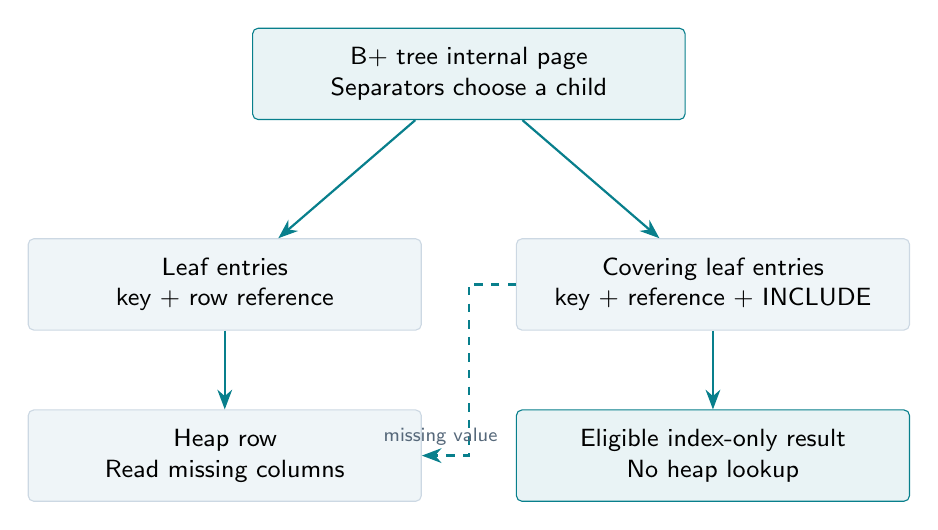
\begin{tikzpicture}[node distance=10mm and 12mm]
\node[strong,text width=50mm] (root) {B+ tree internal page\\Separators choose a child};
\node[box,text width=45mm,below=15mm of root,xshift=-31mm] (leaf1) {Leaf entries\\key + row reference};
\node[box,text width=45mm,below=15mm of root,xshift=31mm] (leaf2) {Covering leaf entries\\key + reference + INCLUDE};
\node[box,text width=45mm,below=of leaf1] (heap) {Heap row\\Read missing columns};
\node[strong,text width=45mm,below=of leaf2] (covered) {Eligible index-only result\\No heap lookup};
\draw[arrow] (root) -- (leaf1);\draw[arrow] (root) -- (leaf2);
\draw[arrow] (leaf1) -- (heap);\draw[arrow] (leaf2) -- (covered);
\draw[arrow,dashed] (leaf2.west) -- ++(-6mm,0) |- node[smalllabel,pos=.8,above] {missing value} (heap.east);
\end{tikzpicture}
\caption{Why a covering index can avoid heap reads. The right branch is available only when every referenced value is recoverable from an eligible index; functional indexes currently remain heap-backed.}
\label{fig:index-access}
\end{figure}

\subsection{Basic and unique indexes}

\begin{lstlisting}[language=SQL]
CREATE INDEX idx_products_stock ON products(stock);
CREATE UNIQUE INDEX ux_products_name ON products(name);
SHOW INDEXES FROM products;
\end{lstlisting}

A normal index permits repeated keys. A unique index adds a uniqueness rule, so create one because the rule is meaningful, not merely because a lookup happens to return one row today. Indexes cost storage and add work to inserts, updates, deletes, maintenance, and recovery. Before adding several indexes, identify the query each one is meant to improve.

Single-column equality and range predicates can use eligible B+ tree paths. The catalog type of the indexed expression and bound query must agree. Avoid gratuitous casts or function wrappers around an indexed column: they can change the bound expression and prevent the intended access path.

The encoded key has a hard 256-byte limit, including type tags, separators, escapes, and the four-byte SQL prefix. A long VARCHAR declaration does not guarantee that every value can be indexed. Variable values containing zero bytes expand under escaping. The leaf payload has a separate 3584-byte limit, independent of database page size. Size keys and included payloads for realistic maximum values, not only an average row.

\subsection{Composite indexes: the current restriction matters}

\begin{lstlisting}[language=SQL]
CREATE INDEX idx_orders_customer_status
ON orders(customer_id, order_status);

EXPLAIN SELECT order_id FROM orders
WHERE customer_id = 1 AND order_status = 'new';
\end{lstlisting}

The current SQL optimizer accepts a composite index for equality on every key column. It does not select a partial leftmost-prefix lookup or a composite range access path. Therefore the index above is not a general replacement for a separate \code{customer\_id} index when the query filters only on that column. This is narrower than the usual textbook description of a B+ tree's theoretical capabilities.

Composite encoding and the tree comparator do understand component boundaries, but a representable range is not automatically an implemented planner path. Use EXPLAIN on the exact predicate. When both full-key and single-column queries are important, compare the benefit and write cost of a separate single-column index.

\sourcecode{src/minisql/planner/optimizer.ml}{chooseIndex requires complete equality for multi-column keys.}

\subsection{Covering indexes with INCLUDE}

\begin{lstlisting}[language=SQL]
CREATE INDEX idx_orders_customer_cover
ON orders(customer_id) INCLUDE (order_id, order_status);

EXPLAIN SELECT order_id, order_status FROM orders
WHERE customer_id = 1;
\end{lstlisting}

INCLUDE columns are stored in leaf payloads. They do not participate in key ordering or uniqueness. Key and included column lists may not overlap. An index-only plan is possible only when the key and included values cover every value required by projections, predicates, grouping, and ordering in the eligible query.

Covering is particularly useful when the omitted heap columns contain large TEXT/BLOB payloads. Projection pruning already avoids loading unreferenced external values during supported scans; index-only access can avoid opening heap/overflow pages entirely. However, including large text values duplicates them in every relevant leaf entry and can exceed the payload bound. Use INCLUDE for compact frequently returned values.

\subsection{Partial indexes}

\begin{lstlisting}[language=SQL]
CREATE INDEX idx_active_customers_city
ON customers(city) INCLUDE (customer_id, name)
WHERE active = TRUE;

EXPLAIN SELECT customer_id, name FROM customers
WHERE active = TRUE AND city = 'London';
\end{lstlisting}

A partial index stores only rows whose predicate is TRUE; FALSE and UNKNOWN/NULL are omitted. Its predicate must be an immutable, row-local Boolean expression. The supported subset uses columns, literals, unary/binary operations, and IS NULL. Functions, subqueries, aggregates, windows, and session-dependent expressions are rejected in this predicate position.

The optimizer proves safety conservatively for single-table plans. It recognizes identical typed conjuncts and certain stronger typed equality/range bounds on the same column. It does not prove arbitrary Boolean equivalence or floating-point bounds. A query can be logically compatible with a partial index and still fall back to another path. Rewriting a query to match the established predicate directly can make the intent clearer, but never weaken the predicate merely to obtain an index plan.

A partial unique index enforces uniqueness only among qualifying rows. It is not an eligible foreign-key target, and the current ON CONFLICT column target cannot infer it because that syntax does not specify a partial predicate.

\subsection{Functional indexes}

\begin{lstlisting}[language=SQL]
CREATE INDEX idx_customers_lower_name
ON customers(LOWER(name));

EXPLAIN SELECT customer_id, name FROM customers
WHERE LOWER(name) = 'ada';
\end{lstlisting}

The current functional index accepts one deterministic row-dependent scalar expression. Casts, literals within that expression, deterministic scalar functions, and unary/binary operations are supported where binding permits them. Constant-only keys, parameters, subqueries, aggregates, windows, and mixed expression/composite keys are rejected.

The query must compare the same typed bound expression with a literal. Functional join probes, expression statistics, and expression-aware index-only decoding are not implemented; matching rows are fetched from the heap. INCLUDE, WHERE, and UNIQUE can be combined with a functional key within their individual restrictions. A quoted identifier whose meaning cannot survive canonical expression serialization is rejected at index creation rather than being persisted ambiguously.

\subsection{Combine access paths without changing correctness}

Eligible independent indexed conjunctions can intersect row-reference sets; fully indexable disjunctions can union and deduplicate them. This is useful when no single index matches a combination well. A residual predicate remains necessary for conditions not guaranteed by the access path. The optimizer also propagates typed non-NULL constants across top-level inner-equality graphs, enabling selective access on related tables. Outer-join inference is deliberately excluded because moving a condition can change which unmatched rows survive.

\sourcecode{src/minisql/planner/optimizer.ml}{Covering decisions, selectivity, access-path combinations, and join order.}
\sourcecode{src/minisql/executor/dml.ml}{Typed index maintenance, partial predicates, functional keys, and INCLUDE decoding.}

\section{Join order and operator behavior}
\index{join algorithms}\index{optimizer}

Connected inner-equijoin graphs of up to eight sources use bounded left-deep dynamic programming. Larger graphs use a deterministic connected greedy fallback. Outer joins retain their SQL order. There is no unrestricted search of bushy join trees.

Use explicit JOIN syntax for clarity. Comma-separated FROM sources are accepted; an equality linking sources can be promoted into the same costed join machinery, while other predicates remain residual filters. This optimization does not rescue a missing join condition: a cartesian product still multiplies rows and can dominate memory and runtime.

A hash join is not universally faster than nested loops. A selective outer input plus a matching index can favor index nested loops; tiny tables may favor a simple nested loop. Large eligible hash joins and grouped aggregates can partition to validated temporary runs and use up to four native workers. Parallelism has startup and partitioning costs, so small tutorial queries should not be expected to use all cores.

For aggregation, scalar COUNT/SUM/AVG/MIN/MAX/BOOL\_AND/BOOL\_OR can use fixed-size streaming accumulators in eligible plans. COUNT(*) can use verified slot metadata. Grouping requires retaining or spilling groups, and STRING\_AGG necessarily accumulates output content. A one-row aggregate result does not mean one row of work.

\section{Memory, temporary files, and result size}
\index{spill}\index{Top-N}

The per-session \code{runtime.temporaryMemoryBytes} setting supplies a soft blocking-operator budget. The engine default is 64 MiB; the accepted minimum is 1 MiB. Sort and hash operators estimate row widths and derive thresholds from bytes rather than treating a short row and a huge row as equivalent. Eligible operations spill to the database's temporary area.

This setting is not a total-process ceiling. Parser objects, unsupported materializing operations, a very wide row, and a compatibility result array can temporarily exceed it. \code{runtime.temporaryStorageBytes} separately limits shared spill reservations. \code{runtime.processMemoryBytes} uses live MiniLang managed-heap accounting at admission and cooperative polling points; native TLS/socket allocations, mapped files, and total RSS remain outside that measure. Set an operating-system limit when a strict process ceiling is required.

Result rows are transmitted in bounded continuation frames, normally at most 512 rows and targeting roughly 1 MiB. The protocol's defensive payload ceiling is 16 MiB; one unsplittable row must still fit. Server max-result-row/byte controls can reject a statement even when its operators stayed within their spill budgets. Client-side fetch size does not override these server bounds.

Eligible simple SELECTs inside CALL emit bounded 128-row execution batches
without retaining completed result sets. Blocking queries, unproved expression
dependencies and dynamic SQL use the ordinary materializing path. The embedded
executeSql API still returns complete QueryResult objects. Direct Python/JDBC
CALL consumers can fetch incrementally; callproc and CallableStatement instead
consume completion to obtain OUT values and spool preceding results to
temporary files for later traversal. Temporary disk capacity and the lifetime
of an unread result therefore remain relevant even when row residency is
bounded. A transport failure stops evaluation and closes its cursor and read
lease; a SQL handler cannot resume work after a failed consumer.

Three independent questions must therefore be answered:

\begin{enumerate}
\item Does the server operator stream or materialize its inputs and result?
\item Does the transport divide the result into bounded frames?
\item Does the application consume incrementally or retain every received row?
\end{enumerate}

A positive answer to only the second question does not bound total memory. Use narrow projections, explicit predicates, and meaningful LIMITs when the application needs only a subset. Avoid SELECT * for exports that intentionally exclude large payloads.

\section{Plan reuse and cache invalidation}
\index{plan cache}

Each engine session has a 64-entry optimizer plan cache. Exact top-level SQL text and canonical nested AST keys are used. Repeating structurally similar SQL with different inline literal text is not the same as guaranteed reuse of one top-level key. Driver prepared statements provide another explicit reuse layer, with their own lifetimes and bounds.

DDL, ANALYZE, VACUUM, and REINDEX invalidate planning context across attached sessions. This prevents a cached plan from silently assuming an obsolete schema or statistics generation. After maintenance, the first query can incur replanning and a cold read-cache path. Measure a representative sequence rather than treating that first execution as a permanent regression.

Cache counters describe implementation activity; they are not guarantees that every part of a query bypassed parsing, binding, authorization, or storage checks. Prepared statements also do not freeze data or isolation behavior.

Each engine also retains at most 64 parsed procedure definitions. This cache
is separate from query plans and is keyed by durable procedure identity,
complete canonical SQL and persisted execution context. ALTER, replacement
and drop/recreate therefore invalidate the matching program. Argument values,
local scopes and privilege decisions are never cached: each CALL checks its
caller and definer again, so a warm cache does not postpone REVOKE.

\section{Concurrency and application design}
\index{concurrency}\index{readers/writer gate}

\begin{figure}[htbp]
\centering
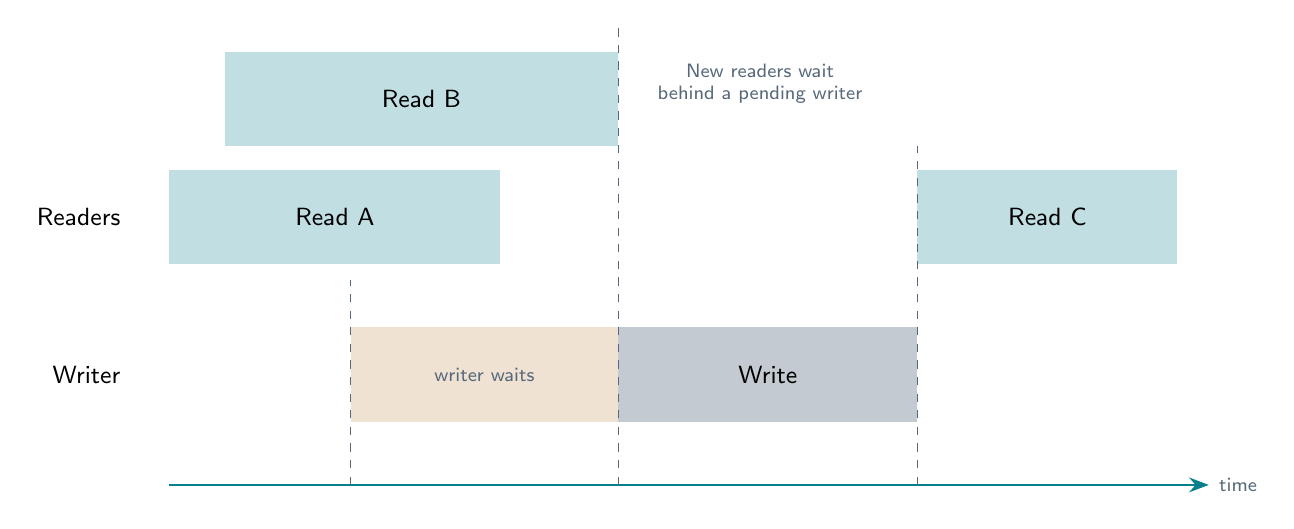
\begin{tikzpicture}[x=1mm,y=1mm]
\node[font=\sffamily\small,anchor=east] at (0,34) {Readers};
\node[font=\sffamily\small,anchor=east] at (0,14) {Writer};
\draw[arrow] (5,0) -- (137,0) node[right,smalllabel] {time};
\fill[Teal!25] (5,28) rectangle (47,40);\node[font=\sffamily\small] at (26,34) {Read A};
\fill[Teal!25] (12,43) rectangle (62,55);\node[font=\sffamily\small] at (37,49) {Read B};
\fill[Amber!18] (28,8) rectangle (62,20);\node[smalllabel] at (45,14) {writer waits};
\fill[Navy!25] (62,8) rectangle (100,20);\node[font=\sffamily\small] at (81,14) {Write};
\fill[Teal!25] (100,28) rectangle (133,40);\node[font=\sffamily\small] at (116.5,34) {Read C};
\draw[dashed,draw=Muted] (28,0) -- (28,26);\draw[dashed,draw=Muted] (62,0) -- (62,58);\draw[dashed,draw=Muted] (100,0) -- (100,43);
\node[smalllabel,align=center] at (80,51) {New readers wait\\behind a pending writer};
\end{tikzpicture}
\caption{The database execution gate permits concurrent ordinary reads and one exclusive writer. This scheduling diagram is separate from SQL transaction isolation and logical locks.}
\label{fig:read-write-gate}
\end{figure}


Each connection occupies a worker in the bounded native connection pool.
Network handling, framing and independent read-only plans can proceed in
parallel. Every database has a writer-prioritized readers/writer execution
gate: ordinary read-only SELECT, EXPLAIN and metadata can be shared, while
ordinary mutations, maintenance and session-state operations are conservatively
exclusive. CALL can share the reader gate only after its complete known body
and callee tree have been proved free of database writes. This proof inspects
expressions and handlers; READS SQL DATA and NO SQL are descriptions, not
authorization to bypass it. Dynamic SQL, sequence mutation, views/subqueries
with unproved dependencies and other unknown operations use the exclusive
path. The separate read-only transaction setting still has the documented
sequence limitation; it is not a general protection against NEXTVAL.

There is one active physical writer per database. Raising maxConnections admits more sessions; it does not create multiple physical writers. When a writer waits, new readers stop entering so it will not starve. Existing readers still need to complete. Long queries, slow result consumers, and long logical transactions can therefore affect other work even when the machine has idle CPU capacity.

Keep application transactions short and purposeful. Do not wait for a user dialog, HTTP call, or lengthy file processing while retaining database locks. Parse and validate an import before or incrementally within a carefully chosen transaction strategy. For very large loads, decide whether all-file atomicity is worth a long transaction or whether independently committed chunks with an explicit restart key better fit the application.

\section{A repeatable tuning exercise}

Use a disposable copy of the tutorial database, and add enough rows to make access differences visible. Preserve query results before and after each change; performance tuning must not change the answer.

\begin{enumerate}
\item Run a filtered SELECT without new indexes. Record wall time and EXPLAIN ANALYZE.
\item Run ANALYZE and compare estimated selectivity with actual output counts.
\item Add one index matching the equality or range predicate. Explain the identical SQL again; a small table may still favor a scan.
\item Add compact INCLUDE columns for a frequent projection. Check whether Index Only Scan appears and whether heap reads decrease.
\item Compare a narrow projection with SELECT * when another column has external TEXT/BLOB values.
\item Compare ordered LIMIT queries against full ORDER BY results. Look for Top-N only when its eligibility conditions are met.
\item Repeat with several simultaneous reader connections, then introduce a controlled writer and measure its waiting time.
\item Remove any experimental index whose measured value does not justify its storage and write cost.
\end{enumerate}

Use the performance and production-control test programs in \path{tests/performance} and \path{tests/integration} as workload examples. Their dated results describe particular earlier revisions and machines; the current storage-v2 development commit must be qualified independently for the intended deployment.

\chapter{Storage Architecture and Formats}
\label{adv:storage}

\section{Why an administrator should understand the files}

SQL users normally manipulate tables, not bytes. Physical knowledge becomes useful when estimating storage, selecting a page size, diagnosing corruption, interpreting a backup, or writing an inspection tool. It also prevents dangerous assumptions: a table is not a single CSV-like sequence of rows, deleting a row need not shrink its file, and a WAL file is not a replayable list of SQL statements.

This chapter describes the current storage-v2 development implementation. The product version string remains 1.1.1, but that does not identify the on-disk generation. Earlier 1.1.1 builds used database format 1. The explicit persisted format fields decide whether a database can open.

\warning{Storage generation 2 is an intentional break}{Format-1 databases and backups containing them are rejected. Editing a version number or configuration value cannot convert their layout. The page-size rewrite tool operates on databases accepted by the current engine and is not a format-1 importer. Preserve an appropriate old engine when extracting data from an older database.}

Unless stated otherwise, numeric fields below are little-endian, offsets are zero-based, and lengths are bytes. UUIDs and text are byte strings rather than endian-swapped integers. Reserved bytes must have the specified zero values; an inspector must validate them rather than inventing meanings.

\begin{longtable}{p{.56\linewidth}p{.33\linewidth}}
\toprule Structure & Current version \\\midrule
Database metadata identity/envelope & 2 \\
User-table header, physical row & 2 \\
Overflow pointer and page payload & 2 \\
B+ tree metadata and nodes, SQL key, INCLUDE payload & 2 \\
Paged-file superblock and common page header & 1 \\
WAL record framing, checkpoint and durable marker & 1 \\
Catalog envelope and generic envelope header structure & 1 \\
Wire protocol & 1 \\
\bottomrule
\end{longtable}

A retained version-1 wrapper does not make its new payload compatible with old engines. For example, a common page header remains version 1 around a version-2 row or index payload. Schema version is another independent number: it tracks compatible column evolution within the physical row generation.

\sourcecode{src/minisql/common/format_version.ml}{Central format-version registry.}
\sourcecode{docs/formats/FORMAT_COMPATIBILITY.md}{Storage-v2 compatibility boundaries.}

\section{Database directory and ownership}

Initialization creates a generated \path{db_<uuid>} directory under the requested root. Use the returned actual path for daemon and offline commands. The friendly SQL database name lives in metadata; it is not the physical directory name.

\begin{longtable}{p{.36\linewidth}p{.55\linewidth}}
\toprule Path or family & Purpose \\\midrule
\path{db.meta} & Database UUID, name, persisted format tuple, page size, and identifier/checkpoint high-water marks. \\
\path{db.lock} & Operating-system-backed ownership/locking coordination. A filename alone is not proof of a live lock. \\
\path{catalog/catalog.tbl} & Bootstrap table/column catalog in a scalable paged representation. \\
\path{catalog/schema.history} & Table schema versions, constraints, defaults, identities, and index-related metadata. \\
\path{catalog/schema.extensions} & Additional schema objects and their durable definitions, as used by the extension layer. \\
\path{catalog/security.tbl}, \path{catalog/security.0.tbl}, \path{catalog/security.1.tbl}, \path{catalog/security.v2} & Security metadata, scalable independently durable generations, and publication marker. These form a coordinated state. \\
\path{tables/t<ID>.tbl} & User-table header, heap pages, and overflow pages. \\
\path{tables/t<ID>.tbl.heap-pages} & Derived checksummed heap-page directory used to accelerate scans. \\
\path{indexes/i<ID>.idx} & B+ tree index file. \\
\path{wal/wal.log} & Transaction records and full page images. \\
\path{wal/checkpoint.meta} & Redundant checkpoint positions. \\
\path{wal/wal.log.durable} & Published durable WAL prefix used by replication. \\
\path{tmp/} & Temporary sort/hash work. \\
\path{audit/} & Audit chain and anchor records when used. \\
\bottomrule
\end{longtable}

The engine also creates pending journals, index-dirty markers, statistics, encryption metadata, and replication/fencing state for the relevant features. Presence depends on the database's history and configuration. Treat a database directory as one coordinated unit. Copying a table, catalog, security generation, or WAL file in isolation does not create a consistent database.

The heap-page directory is derived acceleration metadata. If it is missing, stale, or damaged, the engine rebuilds it by classifying physical pages; it excludes user-table page zero. Do not restore it independently of its table. Authoritative data and derived metadata have different recovery roles, but an operator should still use supported maintenance and backup procedures instead of deleting files while the server runs.

\sourcecode{src/minisql/catalog/catalog.ml}{ensureLayout, generated database paths, catalog and security file ownership.}
\sourcecode{src/minisql/storage/heap_file.ml}{Heap pages, derived directories, and forwarding.}
\sourcecode{src/minisql/catalog/schema_history.ml}{Schema history and extension paths.}

\section{Paged-file wrapper and superblocks}
\index{superblocks}

A paged file starts with two 4096-byte superblock slots, independent of the logical page size. Logical page 0 begins after these 8192 bytes. For an unencrypted file with page size $P$, logical page $n$ starts at
\[
  \mathrm{offset}(n) = 8192 + nP.
\]
The supported $P$ values are 4096, 8192, 16384, and 32768. Increasing page size does not remove every independent per-entry or protocol bound.

Each superblock slot has this layout:

\begin{longtable}{p{.12\linewidth}p{.12\linewidth}p{.65\linewidth}}
\toprule Offset & Bytes & Field \\\midrule
0 & 8 & ASCII \code{MSQLSB01}. \\
8 & 2 & Superblock format version 1. \\
10 & 2 & Header size 128. \\
12 & 2 & File type: table 1, index 2, WAL 3, database metadata 4, generic 255. \\
14 & 2 & Reserved zero. \\
16 & 8 & Generation. \\
24 & 4 & Logical page size. \\
28 & 4 & Reserved zero. \\
32 & 8 & File identifier. \\
40 & 8 & Committed logical page count. \\
48 & 16 & Database UUID. \\
64 & 4 & Feature flags; bit 0 enables page encryption. \\
68 & 4 & Reserved zero. \\
72 & 4 & CRC-32C of the full 4096-byte slot with this field zeroed. \\
76 & 52 & Reserved header bytes. \\
128 & 3968 & Reserved slot bytes. \\
\bottomrule
\end{longtable}

The redundant slots permit generation-based publication and validation of an independently valid slot. The committed page count is the allocation authority; a physical tail beyond that frontier is not automatically committed data. Database/file identity must agree across the selected superblock, page headers, and catalog expectations.

With TDE, the superblocks remain plaintext. Each logical page is stored as 12 nonce bytes, $P$ ciphertext bytes, and a 16-byte GCM tag, giving stride $P+28$. The unencrypted logical-page offsets then refer to the decrypted page contents, not direct byte positions in the ciphertext file. Inspectors must authenticate and decrypt before parsing page headers.

\sourcecode{src/minisql/storage/superblock.ml}{Slot codec, generation selection, and supported identifiers.}
\sourcecode{src/minisql/storage/paged_file.ml}{Physical page offsets, publication, and encryption stride.}

\section{The common page header}
\index{page header}\index{CRC-32C}

Every ordinary logical page starts with a 64-byte header. It protects both identity and content.

\begin{longtable}{p{.12\linewidth}p{.12\linewidth}p{.65\linewidth}}
\toprule Offset & Bytes & Field \\\midrule
0 & 4 & ASCII \code{MSPG}. \\
4 & 2 & Page-header version 1. \\
6 & 2 & Header size 64. \\
8 & 2 & Page type. \\
10 & 2 & Flags. \\
12 & 4 & Reserved zero. \\
16 & 8 & File identifier. \\
24 & 8 & Logical page number. \\
32 & 8 & Page LSN. \\
40 & 8 & Page generation. \\
48 & 2 & Item count. \\
50 & 2 & Free-start offset. \\
52 & 2 & Free-end offset. \\
54 & 2 & Reserved zero. \\
56 & 4 & CRC-32C of the payload, bytes 64 through end of page. \\
60 & 4 & CRC-32C of all 64 header bytes with this field zeroed. \\
\bottomrule
\end{longtable}

Page types are free 0, heap 1, overflow 2, B+ tree internal 3, B+ tree leaf 4, catalog 5, table metadata 6, and generic 255. The payload's own marker and version refine this interpretation. A checksum is not authentication; CRC detects accidental corruption, while encrypted pages additionally use authenticated encryption.

\sourcecode{src/minisql/storage/page.ml}{Header fields and page-type registry.}

\section{User-table page zero}
\index{table metadata page}

A format-v2 user table always reserves logical page 0 for immutable identity metadata. Heap and overflow data begin at page 1. This rule does not apply to catalog/security files merely because they share the paged-file table type.

\begin{longtable}{p{.12\linewidth}p{.12\linewidth}p{.65\linewidth}}
\toprule Offset & Bytes & Field in the decrypted logical page \\\midrule
0 & 64 & Common header, type TABLE\_META (6), page 0, LSN 0, item count 0, free-start 128, free-end $P$. \\
64 & 4 & ASCII \code{MSTB}. \\
68 & 2 & Table format 2. \\
70 & 2 & Occupied header bytes 128. \\
72 & 16 & Database UUID. \\
88 & 8 & Table/file object identifier. \\
96 & 4 & Logical page size $P$. \\
100 & 2 & Checksum algorithm 1, CRC-32C. \\
102 & 2 & Physical row format 2. \\
104 & 8 & Nonzero immutable creation generation. \\
112 & 8 & First permitted data page, 1. \\
120 & 8 & Reserved zero. \\
128 & $P-128$ & Reserved zero tail. \\
\bottomrule
\end{longtable}

Page zero is made durable before data allocation. It intentionally has no mutable page-count hint: the superblock owns that information. The common header generation equals the recorded creation generation and must not exceed the selected superblock generation. Creation, reopen, VACUUM, and page-size rewrite all validate or create this header. A row identifier that points to page zero is invalid.

\sourcecode{src/minisql/storage/table_header.ml}{encode, validatePage, initialize, and checked open paths.}

\section{Heap pages and stable row references}
\index{slotted page}\index{row reference}
\begin{figure}[htbp]
\centering
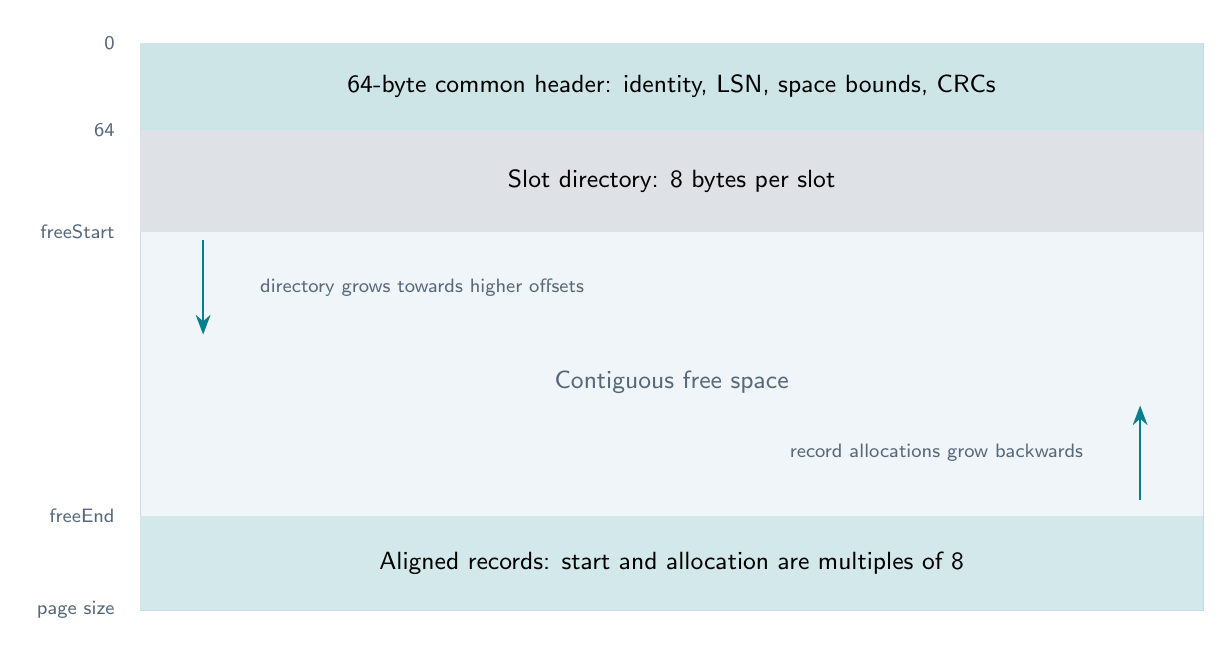
\begin{tikzpicture}[x=1mm,y=1mm]
\draw[draw=Rule,fill=Pale] (0,0) rectangle (135,72);
\fill[Teal!20] (0,61) rectangle (135,72);
\node[font=\sffamily\small] at (67.5,66.5) {64-byte common header: identity, LSN, space bounds, CRCs};
\fill[Navy!14] (0,48) rectangle (135,61);
\node[font=\sffamily\small] at (67.5,54.5) {Slot directory: 8 bytes per slot};
\draw[arrow] (8,47) -- (8,35);\node[smalllabel,anchor=west] at (14,41) {directory grows towards higher offsets};
\node[font=\sffamily\small\color{Muted}] at (67.5,29) {Contiguous free space};
\draw[arrow] (127,14) -- (127,26);\node[smalllabel,anchor=east] at (121,20) {record allocations grow backwards};
\fill[Teal!18] (0,0) rectangle (135,12);
\node[font=\sffamily\small] at (67.5,6) {Aligned records: start and allocation are multiples of 8};
\node[smalllabel,anchor=east] at (-2,72) {0};
\node[smalllabel,anchor=east] at (-2,61) {64};
\node[smalllabel,anchor=east] at (-2,48) {freeStart};
\node[smalllabel,anchor=east] at (-2,12) {freeEnd};
\node[smalllabel,anchor=east] at (-2,0) {page size};
\end{tikzpicture}
\caption{A slotted data page in storage format 2 (schematic, not to scale). Slot identities remain stable when record bodies move during page compaction. Table page 0 has a different metadata layout.}
\label{fig:slotted-page}
\end{figure}


A heap page has a slot directory growing upward from byte 64 and record allocations growing downward from the page end. A slot is eight bytes: U16 record offset, U16 logical record length, U16 state, and U16 generation. Slot $i$ starts at $64+8i$.

\begin{longtable}{p{.17\linewidth}p{.72\linewidth}}
\toprule State & Meaning \\\midrule
0 & Live record. \\
1 & Deleted; offset and length are zero. \\
2 & Forwarding root, retaining the externally referenced row identity. \\
3 & Internal forwarding record. \\
4 & Moved record. \\
\bottomrule
\end{longtable}

These are enumerated states, not flags that may be combined. Every nondeleted allocation starts on an eight-byte boundary and occupies the logical length rounded up to eight bytes. Padding is zero. A row-v2 record already has an aligned length; a short forwarding or other record can need slot-level padding.

The directory size is $8\times\mathrm{slotCount}$, so free-start is $64+8\times\mathrm{slotCount}$. Free-end is aligned. If no deleted slot can be reused, inserting a record requires its rounded allocation size plus another eight directory bytes. On an empty 4096-byte page, a three-byte body occupies eight bytes at offset 4088. A following nine-byte body occupies sixteen bytes at 4072. Two directory entries consume sixteen bytes, leaving $4096-64-16-24=3992$ contiguous free bytes.

Compaction moves record bodies but preserves slot IDs and generations. Deletion advances a slot generation; generation 65535 is retired instead of wrapped. Thus a stale row reference cannot silently identify a new row that reused the same physical slot. A forwarding record retains a stable root when a growing row moves. Its 24-byte \code{MSFW} layout contains version, target page, slot, and generation; resolution rejects cycles and is bounded to 64 links.

\sourcecode{src/minisql/storage/slotted_page.ml}{Slot states, aligned allocation, generation handling, and validation.}
\sourcecode{src/minisql/storage/heap_file.ml}{Stable row identities and forwarding chains.}

\section{Physical row format 2}
\index{row format}\index{binary64}
\subsection{Header, NULL bitmap, and directory}

A row starts at an eight-byte-aligned offset and its total encoded length is a multiple of eight. Its header is:

\begin{longtable}{p{.12\linewidth}p{.12\linewidth}p{.65\linewidth}}
\toprule Offset & Bytes & Field \\\midrule
0 & 4 & ASCII \code{MSRW}. \\
4 & 2 & Row format 2. \\
6 & 2 & Schema version, 1--65535. \\
8 & 2 & Stored column count; codec limit 1--4095. \\
10 & 2 & NULL bitmap bytes, $\lceil C/8\rceil$. \\
12 & 2 & Directory offset, $\mathrm{align8}(16+\lceil C/8\rceil)$. \\
14 & 2 & Reserved zero. \\
16 & variable & NULL bitmap, then zero alignment padding. \\
\bottomrule
\end{longtable}

For column $i$, the NULL bit is bit $i\bmod 8$ of byte $\lfloor i/8\rfloor$, least-significant bit first. Unused bitmap bits are zero. Each eight-byte directory entry contains U16 type code, U16 flags, U16 value offset, and U16 value length. Value offsets are relative to the row start.

Flags are exactly 0 for inline, 1 for NULL, or 2 for an external TEXT/BLOB pointer. A NULL has length zero and the current value cursor, without new alignment padding; its bitmap bit and flag must agree. An empty string instead has flag 0, a clear NULL bit, and length zero. Readers reject combinations such as flag 3, inconsistent bitmap entries, noncanonical offsets, and nonzero padding.

\subsection{Value representations}

\begin{longtable}{p{.08\linewidth}p{.18\linewidth}p{.48\linewidth}p{.12\linewidth}}
\toprule Code & Type & Physical value & Align \\\midrule
1 & BOOLEAN & One byte, 0 or 1. & 1 \\
2 & SMALLINT & Signed 16-bit. & 2 \\
3 & INTEGER & Signed 32-bit. & 4 \\
4 & BIGINT & Signed two's-complement 64-bit. & 8 \\
5 & REAL & Finite IEEE-754 binary64. & 8 \\
6 & DOUBLE & Finite IEEE-754 binary64. & 8 \\
7 & DECIMAL & Signed 64-bit coefficient; scale belongs to schema. & 8 \\
8 & CHAR & UTF-8 with ASCII-space padding to declared byte width. & 1 \\
9 & VARCHAR & UTF-8 bytes. & 1 \\
10 & TEXT & UTF-8 inline or external pointer. & 1/8 \\
11 & BINARY & Exact-width raw bytes. & 1 \\
12 & VARBINARY & Raw bytes. & 1 \\
13 & BLOB & Raw bytes inline or external pointer. & 1/8 \\
14 & DATE & Signed 32-bit epoch-day count. & 4 \\
15 & TIME & Signed 64-bit microseconds. & 8 \\
16 & TIMESTAMP & Signed 64-bit epoch microseconds. & 8 \\
\bottomrule
\end{longtable}

Every non-NULL value begins at its natural alignment; introduced bytes are zero. External pointers align to eight regardless of logical type. After the last value, zero padding brings the entire row to eight-byte length. The U16 lengths/offsets give a maximum aligned encoded row size of 65528 bytes, while the containing page and directory usually impose a lower inline limit.

Both REAL and DOUBLE use eight bytes. REAL is not a four-byte float here. Positive/negative zero, subnormal values, and finite binary64 significands are preserved by the storage codec. NaN and infinities are rejected. Exact storage does not remove the separately documented SQL expression and network-rendering limitations.

\subsection{A complete row example}

For schema version 1 containing BIGINT 1, TEXT \code{Nils}, and BOOLEAN true, the directory begins at 24, the three value offsets are 48, 56, and 60, and the complete row has 64 bytes:

\begin{lstlisting}
4d 53 52 57 02 00 01 00 03 00 01 00 18 00 00 00
00 00 00 00 00 00 00 00 04 00 00 00 30 00 08 00
0a 00 00 00 38 00 04 00 01 00 00 00 3c 00 01 00
01 00 00 00 00 00 00 00 4e 69 6c 73 01 00 00 00
\end{lstlisting}

The first sixteen bytes are the header. Byte 16 is the NULL bitmap; bytes 17--23 align the directory. Three directory entries consume 24 bytes. The BIGINT occupies eight bytes, the text four, and the Boolean one; the final three bytes are padding. An inspector needs the catalog schema for decimal scale and declared widths, not merely the row's type tags.

Compatible schema evolution can leave an older stored column prefix. The decoder accepts that prefix within the same physical generation, and the executor supplies missing trailing columns from schema rules. This is not permission to decode a row-format-1 record with a row-format-2 codec.

\sourcecode{src/minisql/storage/row_codec.ml}{Aligned row encode/decode, type tags, and prefix-compatible decoding.}
\sourcecode{src/minisql/common/float_codec.ml}{Exact finite binary64 conversion.}

\section{Overflow values}
\index{overflow}

The SQL writer externalizes TEXT/BLOB values larger than one quarter of the database page size. Their row directory entry refers to a 48-byte pointer rather than the whole value. The physical maximum length is U32, 4294967295 bytes; transport and configured resource bounds can be much smaller.

\begin{longtable}{p{.12\linewidth}p{.12\linewidth}p{.65\linewidth}}
\toprule Offset & Bytes & External pointer field \\\midrule
0 & 4 & ASCII \code{MSOP}. \\
4 & 2 & Version 2. \\
6 & 2 & Reserved zero. \\
8 & 8 & File identifier. \\
16 & 8 & First overflow page. \\
24 & 4 & Total value length, U32. \\
28 & 4 & Reserved zero alignment; not a high length word. \\
32 & 8 & Owner identifier. \\
40 & 4 & CRC-32C of the complete external value. \\
44 & 4 & CRC-32C of the 48-byte pointer with this field zeroed. \\
\bottomrule
\end{longtable}

An empty external value has no chain and uses UINT64\_MAX as the first-page sentinel. Nonempty chain pages use common type 2. After the 64-byte page header, their payload is:

\begin{longtable}{p{.12\linewidth}p{.12\linewidth}p{.65\linewidth}}
\toprule Offset & Bytes & Overflow page field \\\midrule
64 & 4 & ASCII \code{MSOV}. \\
68 & 2 & Version 2. \\
70 & 2 & Reserved zero. \\
72 & 8 & Owner identifier. \\
80 & 8 & Next page, or UINT64\_MAX at chain end. \\
88 & 4 & Chunk byte length. \\
92 & 4 & Total value length, U32. \\
96 & 4 & Zero-based chunk sequence. \\
100 & 4 & Reserved zero. \\
104 & variable & Chunk bytes, at most $P-104$. \\
\bottomrule
\end{longtable}

Reads validate page identity, owner, sequence, length, checksums, and termination before returning a value. The pointer checksum, each page checksum, and full-value checksum serve different scopes. A valid pointer checksum alone cannot prove the chain is complete.

\sourcecode{src/minisql/storage/overflow.ml}{Pointer, chain encoding, and validated reads.}

\section{B+ tree files and typed keys}
\index{B+ tree}\index{index key encoding}
\subsection{Tree metadata and nodes}

An index uses the same 8192-byte superblock region. Logical pages 0 and 1 contain redundant tree metadata; nodes start at page 2. Metadata uses common page type 3 with flag 32768, zero item count, free-start 128, and free-end $P$.

\begin{longtable}{p{.12\linewidth}p{.12\linewidth}p{.65\linewidth}}
\toprule Offset & Bytes & Tree metadata payload \\\midrule
64 & 4 & ASCII \code{MSBM}. \\
68 & 2 & Version 2. \\
70 & 2 & Unique flag: 1 for unique, otherwise 0. \\
72 & 8 & Tree generation. \\
80 & 8 & Root page. \\
88 & 8 & First leaf page. \\
96 & 8 & Last leaf page. \\
104 & 4 & Entry count. \\
108 & 2 & Tree height. \\
110 & 18 & Reserved zero. \\
\bottomrule
\end{longtable}

An empty tree has zero height/count/references. Publication alternates metadata pages after appending the new node state. Full open verifies the highest valid referenced graph and can fall back to an older independently valid generation when the latest graph is damaged. This is a structural recovery mechanism, not a substitute for backup.

Leaf pages have common type 4 and payload marker \code{MSBL} at 64, version at 68, count at 72, previous/next leaf at 76/84, and entries from 96. Each entry is U16 key length, U16 value length, key bytes, then value bytes. Keys are 1--256 bytes and values 1--3584 bytes. The implementation caps a leaf at ten entries even on larger database pages.

Internal pages have common type 3 and marker \code{MSBI} at 64, version at 68, positive level at 70, separator count at 72, first child at 76, and separator records from 88. A separator is U16 key length, U16 zero, U64 right child, then key bytes. The implementation permits 2--12 children, hence 1--11 separators. A separator is the first key of its right-hand child under the actual key comparator.

\subsection{SQL key envelope and ordering}

A SQL key starts with ASCII \code{MSK} and one version byte 2, followed by one or more typed self-delimiting components. The entire prefix and all components count toward the 256-byte limit.

\begin{longtable}{p{.12\linewidth}p{.27\linewidth}p{.5\linewidth}}
\toprule Tag & Domain & Payload after tag \\\midrule
01 & SQL NULL & None. \\
02 & BOOLEAN & One byte 00 or 01. \\
03 & Integral, DECIMAL, DATE/TIME/TIMESTAMP & Signed 64-bit little-endian value/coefficient/temporal unit. \\
04 & REAL/DOUBLE & Eight little-endian binary64 bytes. \\
05 & Character types & Escaped UTF-8 bytes, then 00 00 terminator. \\
06 & Binary types & Escaped raw bytes, then 00 00 terminator. \\
\bottomrule
\end{longtable}

A zero byte in a variable payload is escaped as 00 FF; the terminator is 00 00. Empty strings are therefore representable and distinct from NULL. Catalog metadata fixes each component's declared type and decimal scale.

Little-endian numbers are not lexicographically ordered. The tree comparator reads their typed numeric meaning. For example, 255 contains \code{FF 00 ...}, whereas 256 contains \code{00 01 ...}; the comparator still orders 255 before 256. There is no persisted sign-bit flip or big-endian transform. Composite keys compare component by component. NULL sorts by its low tag in an index key; SQL ORDER BY NULL positioning is a separate executor concern.

\begin{lstlisting}
INTEGER 1:   4D 53 4B 02 03 01 00 00 00 00 00 00 00
INTEGER -1:  4D 53 4B 02 03 FF FF FF FF FF FF FF FF
INTEGER 256: 4D 53 4B 02 03 00 01 00 00 00 00 00 00
DOUBLE 0.1:  4D 53 4B 02 04 9A 99 99 99 99 99 B9 3F
TEXT Nils:   4D 53 4B 02 05 4E 69 6C 73 00 00
\end{lstlisting}

Floating zero signs are preserved in persisted keys and included values, while numerical comparison treats them as equal for lookup and uniqueness. Raw B+ tree keys outside the reserved MSK family retain bytewise ordering. Leaf values are opaque to the tree's ordering; equal keys use bytewise value ordering even when a value happens to start with MSK.

\subsection{Row references and covering payloads}

An ordinary leaf value is twelve bytes: U32 heap page number at 0, U16 slot ID at 4, U16 slot generation at 6, and U32 table ID at 8. The slot generation detects reuse. An INCLUDE value adds ASCII \code{MSI} at offset 12, version byte 2 at 15, and one typed component per included catalog column from 16 onward. There is no repeated column-name list or count in each payload.

The components use the same tags as keys, without the MSK prefix. Included binary64 values decode directly for index-only scans. The catalog order controls interpretation. A wrong version, incomplete component, extra tail bytes, or a catalog-type mismatch is corruption. Changing an INCLUDE list therefore requires proper index DDL and maintenance rather than editing a leaf payload.

\sourcecode{src/minisql/storage/btree.ml}{Metadata, node capacities, typed comparison, and generation publication.}
\sourcecode{src/minisql/executor/dml.ml}{indexValuePart, physical references, and INCLUDE encoding/decoding.}

\section{Database metadata and scalable catalogs}
\index{catalog}\index{database metadata}

\path{db.meta} is paged file type 4 with file ID 1. Its logical page 0 is common type 5. At page offset 64 is U32 envelope length; the \code{MSDBM001} envelope begins at 68. For an unencrypted file, that envelope begins at physical offset 8260.

The generic envelope header is 32 bytes: eight-byte magic, U16 enclosed-format version at 8, U16 kind at 10, U32 flags at 12, U32 payload length at 16, payload CRC at 20, header CRC at 24, and four reserved zero bytes at 28. The header CRC zeroes its own field. For database metadata, version is 2, kind is 1, flags are zero, and the payload is:

\begin{longtable}{p{.12\linewidth}p{.12\linewidth}p{.65\linewidth}}
\toprule Offset & Bytes & Database metadata payload \\\midrule
0 & 4 & Page size. \\
4 & 4 & Logical WAL segment size. \\
8/\allowbreak10/\allowbreak12/\allowbreak14/\allowbreak16 & 2 each & Database/table/index/WAL/row versions: 2,2,2,1,2. \\
18 & 2 & Text encoding 1, UTF-8. \\
20 & 2 & Collation 1, binary. \\
22 & 2 & Database-name UTF-8 byte length $L$. \\
24 & 8 & Next object ID. \\
32 & 8 & Next transaction ID. \\
40 & 8 & Checkpoint LSN. \\
48 & 16 & Database UUID. \\
64 & 16 & Reserved zero. \\
80 & $L$ & Database-name bytes without terminator. \\
\bottomrule
\end{longtable}

The payload length is exactly $80+L$. The codec permits a nonempty name up to 255 bytes; database creation applies stricter identifier rules first. The persisted identifiers/LSNs use U64 fields but are restricted to the supported nonnegative MiniLang scalar range, at most $2^{60}-1$. Do not infer full-U64 API capacity from physical field width alone.

The bootstrap catalog uses file ID 2 and retains an independent version-1 MSCAT001 envelope. Large catalog envelopes are divided into logical page chunks with a BLB2 header: marker at 64, continuation version at 68, total envelope length at 72, chunk index at 80, page count at 88, chunk length at 96, reserved at 100, and data at 104. The reader checks global size and ordering. Catalogs are not restricted to one page or an obsolete one-MiB snapshot.

Schema-history and schema-extension files retain durable SQL definitions and metadata beyond the bootstrap catalog. DDL publication uses a pending journal with before-images and file-move plans. PREPARED means recovery must restore the prior state; COMMITTED means publication succeeded and cleanup can finish. A maintenance journal uses a related protocol for table replacements. Never decide that a temporary-looking file is disposable without understanding whether it belongs to such a pending operation.

\sourcecode{src/minisql/catalog/metadata.ml}{Database metadata and catalog codecs.}
\sourcecode{src/minisql/catalog/catalog.ml}{Paged catalog continuation and security-generation handling.}
\sourcecode{src/minisql/catalog/schema_history.ml}{DDL publication and durable schema definitions.}

\section{WAL, checkpoints, and recovery boundaries}
\index{checkpoint}\index{WAL}

The WAL contains framed transaction records and complete page images. Its logical segment size does not imply a directory of individual segment files: the implementation stores consecutive records in \path{wal/wal.log}. A record has an 80-byte header:

\begin{longtable}{p{.12\linewidth}p{.12\linewidth}p{.65\linewidth}}
\toprule Offset & Bytes & WAL field \\\midrule
0 & 8 & ASCII \code{MSQLWAL1}. \\
8 & 2 & Version 1. \\
10 & 2 & Header size 80. \\
12 & 2 & Record type. \\
14 & 2 & Flags. \\
16 & 4 & Complete record length. \\
20 & 4 & Payload length. \\
24 & 8 & LSN. \\
32 & 8 & Transaction ID. \\
40 & 8 & File ID. \\
48 & 8 & Page number. \\
56 & 8 & Page LSN. \\
64 & 4 & Payload CRC-32C. \\
68 & 4 & Header CRC-32C with this field zeroed. \\
72 & 8 & Zero for plaintext; \code{TDE1WAL1} for encrypted payload. \\
\bottomrule
\end{longtable}

Types 1--4 are transaction begin, page image, commit, and abort; 5/6 reserve checkpoint begin/end. A page-image payload has the matching complete page identity and LSN. Encrypted payloads add a nonce/ciphertext/tag representation. The unchanged WAL framing version cannot make old-format page images valid in a new-format database.

WAL ordering and flushing determine which acknowledged transactions can be recovered. Recovery uses committed page images and refuses inconsistent middle-of-log corruption; an incomplete terminal record is a different case from arbitrary damage in an otherwise committed prefix. The engine's native recovery tests exercise these boundaries. Storage hardware and the operating system must still honor the requested flush semantics.

Checkpoint metadata is a 512-byte file with two 256-byte slots. Each slot has MSQLCKP1 magic, version/size, generation at 16, checkpoint LSN at 24, redo-start LSN at 32, WAL record count at 40, database UUID at 48, and CRC at 64. The highest valid generation wins. Checkpointing changes the redo starting point; it is not a backup and does not replace the database's data files.

The 32-byte \path{wal/wal.log.durable} marker contains MSWDL001, version/size, a durable prefix LSN at 16, and CRC at 24. It is atomically replaced after WAL flush succeeds. It supports replication's view of a durable prefix; local WAL recovery correctness does not depend on treating that marker as a commit record.

Index state, DDL journals, maintenance journals, schema metadata, and WAL each have specific recovery paths. An index can be rebuilt from authoritative rows; a lost authoritative table cannot be reconstructed from an arbitrary current index set. Restore a verified backup plus the matching supported archive history when data files are irrecoverable.

\sourcecode{src/minisql/transaction/wal.ml}{Record framing, durable-prefix publication, and encrypted payload markers.}
\sourcecode{src/minisql/transaction/recovery.ml}{Committed-page recovery and corruption handling.}
\sourcecode{src/minisql/transaction/checkpoint.ml}{Redundant checkpoint metadata.}

\section{Inspection discipline and remaining format references}

Work on an offline copy, identify the database generation first, and validate wrappers before following offsets. A robust parser should check lengths before allocation; identity, checksum, and reserved fields before interpreting payloads; and cycle/sequence bounds before traversing chains. It should preserve corruption diagnostics instead of silently skipping bytes until another magic string appears.

The repository keeps detailed, separately versioned specifications for additional persisted structures. Use these alongside the current code when implementing specialist inspection tools:

\begin{longtable}{p{.44\linewidth}p{.47\linewidth}}
\toprule Specification under \path{docs/formats/} & Scope \\\midrule
\path{protected-envelope-v1.md} & Generic metadata envelope and checksums. \\
\path{catalog-v1.md}, \path{catalog-bootstrap-v1.md} & Catalog records and bootstrap representation. \\
\path{schema-history-v1.md}, \path{schema-extensions-v1.md} & Schema versions, constraints, views, sequences, triggers, and routines. \\
\path{ddl-journal-v1.md}, \path{maintenance-journal-v1.md} & Atomic publication/replacement recovery. \\
\path{statistics-v1.md} & Statistics-family representation and versioned extensions. \\
\path{security-catalog-v1.md}, \path{audit-log-v1.md} & Authorization metadata and audit chain. \\
\path{encryption-envelope-v1.md} & Encrypted pages, WAL, metadata, and key-related envelope rules. \\
\path{backup-manifest-v1.md}, \path{wal-archive-v1.md} & Backup/archive identity, manifest, and replay boundaries. \\
\path{ha-fencing-records-v1.md} & Epoch and lease fencing state. \\
\path{sort-spill-v1.md} & Validated temporary run files. \\
\path{wire-protocol-v1.md}, \path{secure-transport-v1.md} & Network framing and authenticated transport. \\
\bottomrule
\end{longtable}

A filename ending in v1 can describe a retained format family with newer enclosed records; inspect its explicit version tables. The old row/table/index v1 documents are historical references, not the layouts accepted by this development tree.

\chapter{Practice workshops and worked solutions}
\label{learn:workshops}
\learning{Turn reference knowledge into repeatable tasks: query a business model, change data safely, use parameters, inspect a plan and prove that a backup can be restored. Each workshop includes a result or acceptance condition.}

\section{How to use the workshops}
Start with a fresh teaching database loaded by
\path{docs/manual/examples/01-create-shop.sql}. For query-only workshops the dataset
should remain unchanged. For experiments with schema or administration,
use a separate disposable database. Read the task before looking at its
solution. A correct answer must both produce the intended result and respect
the current implementation's limits.

These workshops deliberately distinguish correctness from speed. A four-row
table is suitable for proving join semantics; it is not suitable for drawing
conclusions about throughput. Likewise, a backup command's success status
proves less than an actual restore followed by a checker run and application
queries.

\section{Workshop 1: a stock and customer report}
\subsection{Tasks}
List all active customers in name order. Identify customers whose city is
unknown. Find the two products with the highest stock. Count the total
stock across all products. Explain why an empty city string and SQL NULL
would produce different answers to \code{COUNT(city)}.

\subsection{Solution}
\begin{lstlisting}[language=SQL]
SELECT customer_id, name
FROM customers WHERE active = TRUE ORDER BY name;

SELECT customer_id, name
FROM customers WHERE city IS NULL ORDER BY customer_id;

SELECT product_id, name, stock
FROM products ORDER BY stock DESC, product_id LIMIT 2;

SELECT SUM(stock) AS total_stock FROM products;
\end{lstlisting}
The active customers are Ada, Grace and Linus. Margaret has an unknown city.
The highest-stock products are USB-C Cable (100) and Notebook (50). Total
stock is 200. \code{COUNT(city)} ignores SQL NULL but counts an empty string
as a non-null value. Unknown and known-empty are different facts.

\subsection{Reasoning check}
A result may coincidentally appear sorted without an \code{ORDER BY}.
That does not make the ordering part of the query contract. If two products
have equal stock, the product identifier in the sort makes the displayed
order repeatable.

\section{Workshop 2: joins and customers without orders}
\subsection{Tasks}
Produce one row per order containing the customer's name. Then produce one
row per customer with an order count, including zero. Finally list only
customers with no orders. Explain why a left join followed by
\code{WHERE o.order\_id IS NULL} answers the last question.

\subsection{Solution}
\begin{lstlisting}[language=SQL]
SELECT o.order_id, c.name
FROM orders o JOIN customers c
  ON c.customer_id = o.customer_id
ORDER BY o.order_id;

SELECT c.customer_id, c.name, COUNT(o.order_id) AS orders
FROM customers c LEFT JOIN orders o
  ON o.customer_id = c.customer_id
GROUP BY c.customer_id, c.name
ORDER BY c.customer_id;

SELECT c.customer_id, c.name
FROM customers c LEFT JOIN orders o
  ON o.customer_id = c.customer_id
WHERE o.order_id IS NULL
ORDER BY c.customer_id;
\end{lstlisting}
The counts are 2, 1, 1 and 0 for customer identifiers 1--4. The final query
returns only Margaret. A matching order's primary key cannot be null.
Therefore the null right-hand key identifies the synthetic unmatched row
created by the outer join. Using a nullable non-key column as the unmatched
test would be unsafe because a real matched row might also contain null.

\section{Workshop 3: aggregates, CTEs and windows}
\subsection{Tasks}
Find the quantity in each order. Name the intermediate aggregate with a CTE,
then join it to orders and customers. Number each customer's orders in order
identifier order. Explain the difference between aggregation and a window
function in the shape of the result.

\subsection{Solution}
\begin{lstlisting}[language=SQL]
WITH units AS (
  SELECT order_id, SUM(quantity) AS unit_count
  FROM order_items GROUP BY order_id
)
SELECT o.order_id, c.name, u.unit_count
FROM orders o
JOIN customers c ON c.customer_id = o.customer_id
JOIN units u ON u.order_id = o.order_id
ORDER BY o.order_id;

SELECT order_id, customer_id,
  ROW_NUMBER() OVER (
    PARTITION BY customer_id ORDER BY order_id
  ) AS customer_order
FROM orders ORDER BY customer_id, order_id;
\end{lstlisting}
The first query returns order quantities 3, 3, 3 and 1. The window query
returns four order rows: Ada's orders are numbered 1 and 2; Grace's and
Linus's orders are numbered 1. An aggregate collapses rows into groups. A
window expression calculates a value across related rows while retaining
the row-level result. Consult the window chapter for the implementation's
fixed-frame behavior; explicit frame syntax is unavailable.

\section{Workshop 4: transactions and targeted changes}
\subsection{Tasks}
Reduce keyboard stock by one. Create a savepoint. Reduce it by two more.
Undo only the second change, verify the stock, then undo the entire
transaction. Explain why the final value must equal its initial value.
Do this in one shell session or one script.

\subsection{Solution and checkpoints}
\begin{lstlisting}[language=SQL]
BEGIN;
UPDATE products SET stock = stock - 1 WHERE product_id = 101;
SAVEPOINT second_attempt;
UPDATE products SET stock = stock - 2 WHERE product_id = 101;
SELECT stock FROM products WHERE product_id = 101;
ROLLBACK TO second_attempt;
SELECT stock FROM products WHERE product_id = 101;
ROLLBACK;
SELECT stock FROM products WHERE product_id = 101;
\end{lstlisting}
The displayed values are 9, 11 and 12. The first rollback restores the
savepoint's state; it does not end the transaction. The final rollback
restores the transaction's initial state. Two independent \code{--query}
commands do not share this state, even if both connect to the same port.

As a second exercise, first \code{SELECT} the rows matching a proposed
\code{UPDATE} or \code{DELETE} condition. Compare their identifiers with
your intention before running the change. This habit catches an omitted
predicate more reliably than checking a large affected-row count afterwards.

\section{Workshop 5: application input and result decoding}
\subsection{Tasks}
Write a Python function that fetches a customer by identifier using a bound
parameter. Close both cursor and connection. Explain the return type of the
identifier. Extend the function to return \code{None} when the customer does
not exist. Keep connection secrets outside source code.

\subsection{Solution}
\begin{lstlisting}[language=Python]
import minisql

def customer_by_id(dsn, customer_id):
    connection = minisql.connect(dsn, autocommit=True)
    try:
        with connection.cursor() as cursor:
            cursor.execute(
                "SELECT customer_id, name FROM customers "
                "WHERE customer_id = ?",
                (customer_id,),
            )
            row = cursor.fetchone()
            if row is None:
                return None
            return {"customer_id": int(row[0]), "name": row[1]}
    finally:
        connection.close()
\end{lstlisting}
The connector returns ordinary non-null result cells as strings, so the
application converts the known integer identifier explicitly. A bound
parameter represents a value; it does not replace a table or column name.
The comma in \code{(customer\_id,)} creates a one-element Python tuple.

The connection context manager in this connector controls a transaction
boundary and does not close the connection. The explicit \code{finally}
block is intentional. With \code{autocommit=True}, this single read does not
leave a lazy explicit transaction open. For a multi-step write operation,
use the transaction pattern in the connector chapter instead.

\section{Workshop 6: investigate an index}
\subsection{Tasks}
Explain a query that looks up a product by primary key. Explain a query that
filters a non-key column. On a separate larger fixture, create a suitable
explicit index, run \code{ANALYZE}, then compare \code{EXPLAIN ANALYZE}
before and after. Record both plan shape and observed work.

\subsection{Procedure}
\begin{lstlisting}[language=SQL]
EXPLAIN SELECT product_id, name
FROM products WHERE product_id = 103;

EXPLAIN SELECT product_id, name
FROM products WHERE stock = 100;

CREATE INDEX idx_product_stock ON products(stock);
ANALYZE products;

EXPLAIN ANALYZE SELECT product_id, name
FROM products WHERE stock = 100;
\end{lstlisting}
The acceptance condition is not a particular millisecond value or a promise
that a five-row table must use an index. You should be able to identify the
selected access path, describe the predicate, and explain the trade-off
between reading the table and using a key followed by heap access. Repeat on
data of realistic size and distribution before drawing a performance
conclusion. The performance chapter covers covering, partial and functional
indexes, the full-equality requirement for composite index access, and
statistics that affect these choices.

\section{Workshop 7: a backup is useful only if you can restore it}
\subsection{Tasks}
Use a disposable teaching database. Stop its server gracefully. Create a
backup into a new location using the exact command in the backup chapter.
Restore into a different new location. Run the offline checker on the
restored database, start it on a different port, and compare table counts
and representative joined results with the source.

\subsection{Acceptance conditions}
Record the source directory, backup path, restored directory, source
revision, storage format, page size and tool exit statuses. If encryption
is enabled, demonstrate that the separately protected matching key is
available. The restored server must produce counts 4, 5, 4 and 6 for the
teaching tables, plus Ada 6 and Grace 3 for the grouped-units query. Make a
small reversible write on the restored copy to prove that it is usable as
the intended writable recovery target.

A successful command that merely creates an archive is not sufficient.
An untested key, missing WAL range or schema-mismatched replication base can
remain invisible until recovery is needed. The goal is to prove a full
procedure without changing the original database.

\section{Workshop 8: explain a current implementation limit}
Choose one of the limitations below and write a short explanation containing
the intended SQL meaning, observed behavior at this revision, an example
that exposes the difference and a practical design response.
\begin{itemize}
\item Scaled-decimal coefficients, arithmetic and wire formatting.
\item A parent-key update that leaves a foreign-key child unchanged.
\item \code{CURRENT\_TIMESTAMP} returning epoch zero.
\item \code{NULLIF(5,NULL)} returning null in this implementation.
\item Automatic identities using the current maximum row value rather than
an independent durable sequence allocator.
\item Text \code{'NULL'} and SQL NULL being ambiguous in legacy protocol-v1
results, while peers negotiating results-v2 preserve the distinction.
\end{itemize}
The worked probe results in the validation appendix are the answer key.
An expert answer states the boundary precisely. For example, binary64 row
storage does not fix decimal arithmetic, and a successful foreign-key
definition does not prove that cascading actions execute. When a future
revision repairs a limitation, rerun the relevant probe and revise both
the warning and the expected result.

\section{A capstone project}
Build a small inventory application around the shop model. It should have
parameterized customer/product lookups, a transaction for an order and its
lines, immutable referenced keys, a documented money representation,
explicit handling of every database error, and a repeatable restore test.
Include a short operator guide with the server mode, credentials source,
resource limits, log location, backup retention policy and stop procedure.
Document the exact MiniSQL revision you used.

Assess the project by asking whether a second person can reproduce it from
the instructions, whether failed operations leave a verified state, and
whether the application can distinguish a known failure from an uncertain
commit after a broken connection. These checks combine language knowledge
with the operational judgement needed to use a database well.
\sourcecode{clients/python/minisql/dbapi.py}{Parameter binding, cursor behavior, lazy transactions and connection lifetime.}
\sourcecode{src/minisql/planner/optimizer.ml}{Costed access paths and the index eligibility rules used in the performance workshop.}

\chapter{Troubleshooting and Reference}
\label{adv:reference}

\section{Use the diagnostic before changing the system}

A useful incident record contains the executable/source revision, persisted storage generation, command line or exact SQL, error code and message, relevant server settings, and the smallest reproduction. Add whether the error occurred during connection, parsing, binding, execution, commit, recovery, or result fetching. The same visible symptom can have different causes at these stages.

Before retrying a failed mutation, determine its transaction outcome. A rejected statement, a failed explicit transaction, and a lost connection after a possible commit are different situations. If the application did not receive the result, do not assume either that nothing happened or that retrying is harmless. Use a business key or idempotent application operation to reconcile uncertain outcomes.

\subsection{Connection problems}

\begin{longtable}{p{.3\linewidth}p{.61\linewidth}}
\toprule Symptom & Investigation and next step \\\midrule
Connection refused & Confirm that minisqld is running and that address/port match its listener. Check daemon startup output before changing credentials. \\
Connection closes during HELLO/authentication & Check trusted versus authenticated versus TLS mode. A password-authenticated client cannot be substituted for a TLS client merely because both encrypt some traffic. \\
Wrong database contents & Check the actual daemon database path. Changing the Workbench label, Python database argument, or JDBC catalog label does not switch server databases. \\
TLS failure & Check TLS 1.3 support, required cipher/group, expected server name, certificate dates/trust, correct pin, and the platform credential format. \\
Password rejected & Check principal spelling, enabled/login state, credential source, and endpoint. Do not repeatedly modify users on a different local database. \\
Native client stalls in an older Windows console server & Leave console selection/mark mode with Esc; current daemon code disables QuickEdit, but an older running binary can still be paused by text selection. \\
New statements fail while fetching a prior result & Consume or close the active cursor/ResultSet. Protocol v1 is ordered and does not multiplex unread results. \\
\bottomrule
\end{longtable}

Use the native \code{--ping} family matching the listener before testing a complex query. A successful ping proves an operational connection, not sufficient privileges for every object. A socket read timeout is a client-side deadline; it does not prove that the server rolled back a completed statement.

\subsection{SQL and data problems}

\begin{longtable}{p{.3\linewidth}p{.61\linewidth}}
\toprule Symptom & Explanation and response \\\midrule
An apparently ordinary name causes a syntax error & It may be a reserved keyword. For example, use the tutorial's \code{order\_status}, or explicitly quote an intended identifier. Recheck the grammar at the failing token. \\
An index exists but the plan scans & Check selectivity, ANALYZE, exact expression/type binding, covering requirements, and supported access shape. Composite indexes currently need equality on all key columns. \\
DECIMAL 3.30 displays as 330 & The formatter emits its scaled coefficient. Apply the known schema scale in the client; generic expression scale is not transmitted. \\
DECIMAL arithmetic/comparison surprises & Exact input/storage does not imply correct scale-aware operations in this revision. See Section~\ref{sql:decimal-caveat}; use tested integer units or application decimal arithmetic. \\
DATE/TIME/TIMESTAMP comparison fails & Temporal storage and conversions exist, but current scalar comparison is incomplete. Use the SQL chapter's documented integer-unit alternative where comparisons are required. \\
CURRENT\_TIMESTAMP is zero & This implementation returns epoch zero; provide an application timestamp instead of relying on a real-time default. \\
Text equal to NULL becomes a null in the connector & Wire v1 has no NULL bitmap and uses the token NULL. Project an explicit null indicator when the distinction matters; see Section~\ref{adv:wire-null}. \\
Correlated NOT EXISTS reports runtime error 1306 & A current executor defect produces a missing-struct-member diagnostic. A suitably equivalent LEFT JOIN with a non-nullable joined-key IS NULL test is the documented workaround; ordinary EXISTS and IN subquery support should not be confused with this defect. \\
NULLIF with a NULL second operand is surprising & Current evaluator behavior differs from ordinary SQL expectations in this case; consult the function reference and avoid relying on the unsupported semantic edge. \\
A parent-key UPDATE leaves an orphan child & Incoming foreign-key checks/actions are incomplete. Keep referenced keys immutable and validate existing relationships explicitly. \\
ON DELETE CASCADE/SET NULL fails & The action is parsed and stored but is not implemented as a working cascade. Perform a deliberately ordered, transactional application operation using supported DML. \\
A script stops halfway & The script client stops at the first error. Earlier autocommit statements remain committed. Inspect state before rerunning; scripts are not implicit transactions. \\
A large native script cannot be read & Native script/source reading has a 1 MiB file bound. Split scripts or import through bounded connector batches. \\
\bottomrule
\end{longtable}

These are implementation observations, not merely syntax limitations. Some constructs are accepted by the parser and still have narrower execution behavior. The manual's explicit caveats take precedence over generic SQL tutorials and broad historical feature summaries.

\subsection{Transaction, capacity, and storage problems}

If a transaction has failed, issue ROLLBACK before attempting normal work, unless a supported savepoint recovery path was deliberately established. A second BEGIN is not a general reset operation. In Python, remember that DDL/maintenance can commit earlier DML through the connector's classification; in JDBC, move schema work to autocommit mode yourself.

For slow or blocked work, use an administrative SHOW PROCESSLIST and SHOW STATUS connection. Distinguish a logical lock wait from the database's physical reader/writer gate. Increasing connection count cannot add concurrent physical writers. Cancellation is cooperative and can wait until the next storage-page or DML-row polling point. A long native call or scalar expression may delay that point.

A resource-limit failure can mean statement bytes, response frame size, total result rows/bytes, temporary storage, or managed-heap pressure. Read the complete message and current limits. Increasing every limit at once hides the cause. First narrow a projection, bound a query, release an unread result, or split an import if that matches the application's need. Use OS measurements for total RSS rather than interpreting the managed-heap limit as all allocated process memory.

For corruption or format rejection, stop using the questionable copy for writes, preserve the diagnostic, and run the offline checker on an appropriate stopped database or isolated copy. A format mismatch is not a checksum problem. Never edit the version field to make a file appear current. For an actual corrupt authoritative file, use a verified backup and compatible recovery chain. REINDEX rebuilds indexes; it cannot recreate lost heap rows.

\section{Stable error-code reference}
\index{error codes}

The following registry is part of the observable MiniSQL API. Native clients commonly print \code{ERROR code: message}; connectors map selected codes into language-specific exception types. The module/operation text after the code often supplies the decisive context.

\begin{longtable}{p{.1\linewidth}p{.27\linewidth}p{.52\linewidth}}
\toprule Code & Name & Interpretation / first response \\\midrule
0 & Ok & Success. \\
9000 & NotImplemented & A code path is not implemented; choose a documented alternative. \\
9001 & InvalidArgument & Check API/CLI inputs and bounds. \\
9002 & InvalidConfiguration & Correct the identified configuration field or relationship. \\
9003 & UnsupportedFormat & Verify format generation, flags, and engine compatibility. \\
9004 & CorruptData & Preserve evidence and check the stopped database/copy. \\
9005 & IoFailure & Check path, permissions, free space, and underlying storage diagnostics. \\
9006 & ProtocolFailure & Check matching client/server mode and complete framing diagnostics. \\
9007 & LockConflict & Inspect concurrent ownership/locks and transaction scope. \\
9008 & ClosedHandle & Do not reuse a closed connection, engine, or storage handle. \\
9009 & BufferPoolExhausted & Review buffer use and pinned resources. \\
9010 & PinnedPage & A requested operation conflicts with a pinned page. \\
9011 & TransactionState & Inspect active/failed transaction state; roll back as required. \\
9012 & ReadOnlyViolation & A writable operation was attempted in read-only state. \\
9013 & ObjectExists & Inspect the existing object before retrying creation. \\
9014 & ObjectNotFound & Verify name, schema, endpoint, and object lifetime. \\
9015 & PageFull & A physical record/allocation cannot fit; review row width and supported externalization. \\
9016 & RowNotFound & The targeted physical row is unavailable. \\
9017 & TypeMismatch & Correct type, range, scale, or conversion. \\
9018 & StaleReference & A physical row reference no longer has the expected slot generation. \\
9019 & SqlSyntax & Inspect grammar and the failing token. \\
9020 & BindingError & Resolve names, types, scope, or unsupported bound expression shape. \\
9021 & ConstraintViolation & Read the violated NOT NULL/CHECK/reference/other rule. \\
9022 & DuplicateKey & A primary/unique key conflicts; inspect the business key. \\
9023 & DdlState & DDL context, publication, or transaction state is invalid. \\
9024 & IndexCorrupt & Check/rebuild the affected derived index through supported procedures. \\
9025 & UnsupportedSql & The syntax or execution shape is outside implemented SQL. \\
9026 & NetworkFailure & Inspect transport connectivity and possible transaction outcome. \\
9027 & AuthenticationFailed & Verify credentials and principal state. \\
9028 & AuthenticationRequired & Use a matching authenticated session. \\
9029 & PermissionDenied & Review principal, role memberships, and required grant. \\
9030 & SecurityState & Security metadata or state is inconsistent. \\
9031 & ArchiveState & Backup/archive/replication identities or sequence disagree. \\
9032 & LockTimeout & A logical lock wait exceeded its deadline. \\
9033 & StandbyState & The standby cannot execute the requested writable operation. \\
9034 & TlsFailure & Native TLS setup or transport validation failed. \\
9035 & QueryCancelled & An administrative cancellation token was observed. \\
9036 & QueryTimeout & The absolute cooperative query deadline expired. \\
9037 & ResourceLimit & A configured memory, spill, result, or related resource bound was exceeded. \\
9038 & Write-fence rejection & Leadership lease or epoch no longer permits mutation; check the active primary and fencing state. This code is defined outside the central registry. \\
\bottomrule
\end{longtable}

\sourcecode{src/minisql/common/errors.ml}{Central stable error-code registry through 9037 at the documented revision.}
\sourcecode{src/minisql/server/database_manager.ml}{Fenced-primary mutation rejection uses additional code 9038.}

\section{Capability matrix for migration planning}
\index{compatibility}\index{unsupported features}

Use this matrix when porting an application from another database. ``Implemented'' means the stated subset exists, not that all constructs in another vendor's dialect work. Behavioral exceptions in the SQL chapters remain part of the contract.

\begin{longtable}{p{.27\linewidth}p{.64\linewidth}}
\toprule Area & Current implementation and boundary \\\midrule
Platforms & Native Windows x64 and Linux x64 command-line applications; graphical Workbench is Windows-only. \\
Database selection & One database per listener endpoint; initialization is an administrative tool operation. No SQL CREATE DATABASE or USE workflow. \\
Schemas & Two-part names and public/information\_schema; no configurable search path or three-part catalog qualification. \\
Tables and types & Implemented scalar/text/binary/temporal types, constraints, defaults, identity aliases, stored generated columns; temporal and DECIMAL expression caveats apply. \\
Schema evolution & Supported ALTER operations with dependency/data restrictions; no unrestricted arbitrary type rewrite. \\
DML & INSERT VALUES/SELECT, UPDATE, DELETE, RETURNING, ON CONFLICT, and bounded MERGE form. \\
Foreign keys & Child-reference validation and restrictive parent deletion; parsed cascading actions and parent-key updates have the limitations documented above. \\
Queries & Filtering, ordering, grouping, aggregates, joins including outer forms, derived tables, and set operations in the documented grammar. \\
Subqueries & Scalar, EXISTS, IN, and NOT IN; correlation requires qualified outer references and is limited to supported non-grouped contexts. \\
CTEs & Nonrecursive and recursive anchor plus one UNION/UNION ALL recursive term; no mutual recursion; 10000-iteration guard. \\
Windows & Ranking, navigation, and aggregate windows over complete partitions; no explicit ROWS/RANGE/GROUPS frames or named windows. \\
Views & Stored SELECT definitions; no materialized-view refresh system. \\
Triggers & Row BEFORE/AFTER INSERT/UPDATE/DELETE with one supported DML body and read-only OLD/NEW; recursion depth is bounded to eight. \\
Procedures & Typed positional input parameters and one persisted DML body; no general procedural language or user-defined functions. \\
Sequences & Persisted sequences with session current-value behavior; current evaluation can consume values before per-row execution, so do not rely on NEXTVAL in a SELECT to allocate one distinct value per output row. The cursor-probing path has gaps in read-only and exclusive classification; NEXTVAL can consume twice and can mutate inside BEGIN READ ONLY. Do not rely on those boundaries for sequence use; see the sequence and transaction chapters. Numbering is not gapless. \\
Prepared statements & SQL PREPARE/EXECUTE/DEALLOCATE and connector support; no typed wire parameter-binding frame. \\
Transactions & Explicit/autocommit, savepoints, READ COMMITTED and SERIALIZABLE, supported read-only state; no cross-database transaction or XA coordinator. \\
Concurrency & Parallel connections and eligible independent reads; one physical writer per database. \\
Indexes & B+ tree normal/unique, INCLUDE, partial predicates, and single functional expression within documented restrictions. \\
Composite access & Full-key equality; generic leftmost-prefix and composite range access are not selected by the current SQL optimizer. \\
Planning & Costed scans/joins/aggregates/sorts, bounded inner join reorder, sampled statistics, generation-safe session cache; no optimizer hint language or unrestricted plan search. \\
Administration & Status/process list, SHUTDOWN, cancellation, deadlines, logs/binlog, and configured resource controls. \\
Security & Users/roles/grants, password authentication, protected framing, native TLS, audit, and at-rest encryption workflows. \\
Backup/recovery & Physical backup/restore/check, supported archive/PITR, recovery journals, and offline page-size rewrite; no format-1 conversion in the current engine. \\
Replication/HA & Asynchronous existing-schema WAL replication, standby, fencing, and single-host reference controller; no distributed consensus or synchronous quorum commit. \\
Import/export & SQL scripts, connector programs, Workbench CSV output and clipboard staging; no SQL COPY/LOAD DATA command. \\
Drivers & Python DB-API and Java JDBC; no ODBC or separate HTTP SQL service. \\
Results & Text protocol with string/NULL ambiguity and conservative type metadata; in-process results retain SQL value types. \\
\bottomrule
\end{longtable}

\sourcecode{docs/release/LIMITATIONS.md}{Cross-component scope inventory, checked against the source and explicit caveats in this manual.}

\section{Useful hard bounds and their scope}
\index{limits}

A physical format bound, configured operational limit, and client convenience limit answer different questions. For example, a U32 overflow length does not mean a 4-GiB value can be transmitted in one protocol row.

\begin{longtable}{p{.4\linewidth}p{.49\linewidth}}
\toprule Bound & Value and scope \\\midrule
Database logical pages & 4096, 8192, 16384, or 32768 bytes. \\
Aligned physical row size & At most 65528 bytes by row U16 fields, additionally limited by its page. \\
Row codec column count & 1--4095; not a promise that every such wide row fits a page or result. \\
External value length & U32, at most 4294967295 bytes; other budgets apply. \\
Encoded B+ tree key & 256 bytes including SQL prefix/tags/escaping. \\
B+ tree leaf value & 3584 bytes including row reference and INCLUDE payload. \\
Leaf/internal node capacity & At most 10 entries / 12 children in the current tree implementation. \\
Protocol header/payload & 32-byte header; 16777216-byte defensive payload ceiling. \\
Protocol result frame & At most 1024 columns and normally at most 512 rows; byte limits also apply. \\
Native script file & At most 1048576 bytes read by --script or shell source. \\
Execution scan batch & 128 rows in supported engine batch paths. \\
Optimizer plan cache & 64 entries per session. \\
Python prepared-plan cache & 128 entries per connection. \\
Connector insert coalescing & 256 rows and 768 KiB SQL per combined request. \\
ANALYZE sample & At most 8192 uniformly spaced rows; exact population count. \\
Join-order dynamic search & Up to eight eligible connected inner-equijoin sources. \\
Eligible hash partition workers & Up to four native workers. \\
Recursive CTE guard & 10000 iterations. \\
Trigger recursion guard & Eight nested trigger executions. \\
Heap forwarding resolution & At most 64 links, with cycle rejection. \\
Workbench history/results & 100 history items and 32 result tabs. \\
Workbench browse/paste & Default page 100; browse maximum 1000; paste at most 1000 inserts. \\
\bottomrule
\end{longtable}

Configured server limits can be stricter. Consult the configuration chapter and SHOW STATUS for effective settings rather than treating a compiled protocol maximum as the active deployment policy.

\sourcecode{src/minisql/protocol/constants.ml}{Frame limits, continuation flag, and message registry.}
\sourcecode{src/minisql/storage/btree.ml}{Physical index entry and node limits.}
\sourcecode{src/minisql/executor/executor.ml}{Cache, scan, recursion, and trigger bounds.}

\section{Wire protocol anatomy for implementers}
\index{wire protocol}

A client implementing MiniSQL directly must validate the entire frame, not just read SQL text from a socket. The 32-byte little-endian header contains:

\begin{longtable}{p{.12\linewidth}p{.12\linewidth}p{.65\linewidth}}
\toprule Offset & Bytes & Field \\\midrule
0 & 4 & ASCII MSQL. \\
4 & 2 & Protocol version 1. \\
6 & 2 & Message type. \\
8 & 4 & Flags. \\
12 & 4 & Request ID. \\
16 & 4 & Payload length. \\
20 & 4 & Payload CRC-32C. \\
24 & 4 & Header CRC-32C with this field zeroed. \\
28 & 4 & Reserved zero. \\
\bottomrule
\end{longtable}

Types 1--9 are HELLO, QUERY, PING, CLOSE, AUTH\_BEGIN, AUTH\_CHALLENGE, AUTH\_PROOF, AUTH\_OK, and CANCEL. Types 100--102 are RESPONSE, PONG, and ERROR. Response statuses distinguish command, rows, and error. Flag 1 marks authenticated protected framing; flag 2 means another continuation response with the same request ID follows. Each row frame repeats column information, and the client must reject an unexpected schema or request ID.

HELLO advertises \code{session=<positive-u32>} in its informational message. CANCEL carries a four-byte U32 target session ID and is sent on a separate administrator connection. Its acknowledgement confirms that the cooperative token was set, not that arbitrary native work was synchronously terminated. Older v1 clients can continue interpreting HELLO as text, but an old server without a session identifier cannot supply this cancellation feature.

Password authentication also enables directional authenticated encryption for subsequent MiniSQL frames, including when TLS supplies an outer transport. Implementations must follow nonce/sequence/key-direction rules in the secure-transport specification; do not substitute CRC as an authentication mechanism. Most applications should use the maintained connectors instead of reimplementing this protocol.

\sourcecode{src/minisql/protocol/constants.ml}{Message types, statuses, flags, and payload limits.}
\sourcecode{src/minisql/protocol/messages.ml}{Payload codecs and validation.}
\sourcecode{docs/formats/wire-protocol-v1.md}{Framing and cooperative cancellation extension.}

\section{Glossary}
\index{glossary}

\begin{longtable}{p{.25\linewidth}p{.66\linewidth}}
\toprule Term & Meaning in this manual \\\midrule
Affected rows & Rows changed by a command, distinct from rows returned by a SELECT or RETURNING result. \\
Autocommit & A statement executes without a user-opened multi-statement transaction; connector defaults can differ. \\
Binder & Resolves names, scopes, and types after parsing. \\
Catalog & Metadata describing database objects; JDBC's catalog label is not a database-switch command. \\
Checkpoint & Durable recovery position that bounds later redo work. \\
Collation & Ordering/comparison rule for text; the persisted default is binary. \\
Covering index & An index containing all values required by an eligible query, including INCLUDE columns. \\
CRC-32C & Castagnoli cyclic redundancy check used to detect accidental corruption. \\
DDL / DML / DCL & Definition, data manipulation, and access-control statements respectively. \\
Durable & Written using the engine's required flush/publication protocol, subject to the storage stack honoring those operations. \\
Epoch unit & Integer day or microsecond count relative to a defined origin; not an implicitly timezone-aware timestamp. \\
Execution gate & Per-database coordination of shared readers and exclusive operations. \\
Foreign key & A declared relationship requiring a referenced key; this revision's referential-action limitations must be observed. \\
Heap & Table storage organized around pages and slots, without primary-key clustering. \\
Identity & A generated column value intended for identifiers; not a promise of gapless business numbering. \\
Index-only scan & Query access that obtains needed values from an index without heap reads. \\
LSN & Log sequence number locating/order-identifying WAL state. \\
NULL / UNKNOWN & Missing SQL value and its three-valued Boolean consequence. \\
Overflow & External page chain holding a large TEXT/BLOB value. \\
Partial index & Index containing only rows whose stored predicate is TRUE. \\
Physical row reference & Heap page, slot, and generation information locating a stored row. \\
PITR & Point-in-time recovery using a compatible base archive and available committed WAL history. \\
Prepared statement & A named session statement used with supplied values; not a frozen result. \\
Principal & User or role participating in authorization. \\
Residual predicate & A filter still evaluated after an access path or join has narrowed candidates. \\
Savepoint & A named position for supported partial rollback inside an explicit transaction. \\
Schema version & Evolution of a table definition, distinct from database/row physical format generation. \\
Selectivity & Fraction of rows estimated or observed to satisfy a condition. \\
Spill & Temporary disk representation used by an operator to reduce its retained memory. \\
Standby & Database endpoint serving supported reads while applying compatible replicated history. \\
Superblock & Redundant paged-file metadata slot describing identity and committed allocation. \\
TDE & Transparent data encryption of the supported stored structures. \\
TLS & Transport Layer Security; distinct from MiniSQL's inner authenticated framing. \\
WAL & Write-ahead log used for page-change durability/recovery; not the optional SQL binlog. \\
\bottomrule
\end{longtable}

\section{Read validation evidence precisely}

The historical release gate and the current storage-v2 checks are different evidence. The repository's storage-v2 report records five focused format suites and selected Linux-native regressions, while explicitly stating that the full historical Windows release matrix was not rerun for that change. A successful compile for another target is not a native execution test.

The examples and additional probes delivered with this manual identify their own tested source revision and scope. They improve confidence in the documented learning path and expose known behavior; they do not certify every possible SQL query, driver framework, hardware failure, or production workload. Preserve reproducible test inputs and actual diagnostic output when extending MiniSQL, and update both capability descriptions and limitations when behavior changes.

\sourcecode{docs/acceptance/STORAGE_V2_2026-11-24.md}{Current format-focused validation scope and historical/platform boundaries.}

\appendix
\chapter{Validation, source map and reproducibility}
\label{appendix:validation}

\section{What was checked for this edition}
The implementation reference and source links are pinned to revision
\texttt{\SourceShort}; its full identifier is recorded in \path{edition.tex}.
The original tutorial and recovery examples were
checked with newly built Linux x64 programs from the earlier baseline
\texttt{9bedab0c9de307d0435d3abfb3eab98a2f6d42a5}, using
MiniLangCompilerPy 1.3.10 at compiler revision
\texttt{8e64c9cfda92199b68ac5d3974fea445f12f6c39}.
The server, native client, consistency checker and backup tool were compiled
for the validation. Each run used fresh, disposable database directories.
No existing user database was used as a mutable test fixture.

The manual validation runner executes four complete SQL files through the
native console and checks 53 focused outcomes through the repository's Python
connector. A separate recovery runner verifies the offline backup/restore
procedure, runs the native checker before backup and after restore, starts
the restored database, compares counts and a joined aggregate, and verifies
a writable transaction followed by rollback.

The initial stored-procedure language expansion retains its separate evidence
at revision \texttt{139eb3c}. The subsequent five-package expansion at this
edition's implementation passes 12 focused native Linux cases, including
127 runtime, 21 edge, 154 security/metadata and 105 final parity assertions.
The complete focused run included 100 parity assertions; a later targeted
105-assertion run verifies the final character-set/collation SQLSTATE correction.
Native protocol and authenticated-protocol regressions also pass. Six routine
test programs cross-compile to PE32+ AMD64, and the final parity program is
rebuilt separately after that correction. Windows server, console and
Workbench entry points also cross-compile with validated PE32+ AMD64 images.
No Windows executable was run.

Connector checks pass 18 Python unit tests, 16 general JDBC checks and
77 procedure-specific JDBC checks. Java execution uses Java 21 with
source/target 11 compilation; it is not Java 11 runtime acceptance. A freshly
rebuilt native server passes 33 top-level connector checks, one of which runs
the 25-check JDBC live suite. These two live counts are not additive.
The complete incremental evidence, source hashes and final application-build
results are in \path{docs/acceptance/stored-procedures-2026-11-25.json}.
Historical tutorial and initial procedure records have not been relabeled as
new executions at the current revision.

\begin{longtable}{p{.29\linewidth}p{.63\linewidth}}
\caption{Documentation validation and its limits}\\
\toprule Area & Evidence and interpretation\\\midrule\endhead
Teaching setup & Four tables and 19 data rows loaded through the native script client. Counts are 4 customers, 5 products, 4 orders and 6 order items.\\
Queries & Filtering, sorting, NULL counts, joins, grouped totals, outer-join anti-matching, CTEs, recursion, windows, working subquery shapes and expected results.\\
Changes & Insert/update/delete with RETURNING, savepoint rollback, full rollback, duplicate-key rejection, missing-parent rejection and CHECK rejection.\\
Known limitations & Decimal scaling/presentation, temporal comparison, CURRENT\_TIMESTAMP, NULLIF, legacy text NULL ambiguity, unsupported DELETE CASCADE, orphan-producing parent-key updates, correlated NOT EXISTS, identity reuse and per-row sequence materialization.\\
Operational recipe & Clean stop, native checker, offline backup, restore to a new path, checker on the restored copy, restarted SQL and reversible write.\\
Source review & Parser/binder/executor, command entrypoints, config, security, drivers, Workbench, planner, storage, recovery and replication implementations.\\
Not a claim of execution & This work did not run the full Windows acceptance suite, Windows Workbench, all TLS certificate scenarios, long-duration soak, every replication failure scenario or every SQL combination. Those descriptions are source-reviewed and linked to relevant tests.\\\bottomrule
\end{longtable}

\warning{A passing limitation probe is not a correctness endorsement}{Some
checks deliberately assert an observed defect or unsupported behavior. Such a
check passes when the manual describes the running implementation faithfully.
For example, confirming that \code{NULLIF(5,NULL)} returns null does not make
that result standard-conforming. When the engine changes, a failed limitation
probe may indicate that a warning can be removed after investigation.}

\section{Reproduce the teaching checks}
From the repository root, with matching native executables already built:
\begin{lstlisting}[language=bash]
python3 docs/manual/tools/validate_examples.py \
  --bin-dir build/bin-linux \
  --output build/manual-validation.json

python3 docs/manual/tools/validate_recovery.py \
  --bin-dir build/bin-linux \
  --output build/manual-recovery-validation.json
\end{lstlisting}
On Windows use \code{python} and \path{build/bin}. The runners discover a
free loopback port, create temporary directories under \path{build/}, start
and stop their own processes, and remove their disposable databases when
finished. They do not need a running application server and must not be
pointed at a production database. \code{--bin-dir} selects executables, not
a database path.

The committed \path{validation.json} and \path{recovery-validation.json}
retain the original tutorial/recovery outcomes. They record their source baseline,
platform, script output, expected values and observed results. Rerun with an
output under \path{build/} while comparing a new revision; replace the
committed evidence only as part of a reviewed documentation update.

\section{Selected observed edge cases}
The table below preserves the tutorial-baseline probes. Read the corresponding
language and operations chapters for current explanations and practical
workarounds. In the present procedure expansion, negotiated results-v2 fixes
the literal-NULL ambiguity, and cursor admission no longer evaluates NEXTVAL
once during a probe and again during fallback. Those new regression results
are recorded separately; the historical observations below are unchanged.

\begin{longtable}{p{.45\linewidth}p{.47\linewidth}}
\caption{Recorded tutorial-baseline boundary cases reviewed for this edition}\\
\toprule Probe & Observed outcome\\\midrule\endhead
\code{CAST('3.30' AS DECIMAL(10,2))} & Wire cell \code{330}; the schema scale is not applied by the generic formatter.\\
Add decimal 3.30 and 1.20 & Wire cell \code{45000}; arithmetic adds raw coefficients and rescales incorrectly.\\
Compare decimal 3.30 to integer 330 & \code{TRUE}; mixed-scale comparison is not a reliable numeric comparison.\\
\code{NULLIF(5,NULL)} & SQL NULL.\\
Compare two \code{CAST(0 AS DATE)} values & Error: values are not comparable.\\
\code{CURRENT\_TIMESTAMP} & Wire cell \code{0}, not the current wall-clock time.\\
\code{5 / 2} & \code{2.5}; division deliberately produces a floating result.\\
\code{SELECT 'NULL', NULL} through Python & Both values appear as Python \code{None}.\\
Delete referenced parent with DELETE CASCADE & Rejected with an implementation-stage diagnostic.\\
Update parent key from 1 to 2 with existing child & Update succeeds; child remains at 1.\\
Correlated EXISTS and scalar COUNT subquery & Correct expected fixture results in the tested shapes.\\
Correlated NOT EXISTS & Runtime error 1306: \code{Struct has no member 'kind'}.\\
Sequence starts at 1; query NEXTVAL over products ordered by key & Five rows all display 2; evaluation is not once per row and the cursor/fallback path consumes twice.\\
Next standalone NEXTVAL on that sequence & 4, reflecting the same double-materialization path.\\
BEGIN READ ONLY; NEXTVAL; ROLLBACK & NEXTVAL succeeds with 6; CURRVAL remains 6 after rollback.\\
Identity rows 1,2; delete 2; insert again & The new row reuses 2 because allocation uses the current maximum.\\\bottomrule
\end{longtable}

\section{How the manual covers the repository}
\begin{longtable}{p{.28\linewidth}p{.64\linewidth}}
\caption{The implementation areas behind the handbook}\\
\toprule Area & Primary files and corresponding chapters\\\midrule\endhead
Build and applications & \path{build.ps1}; all six \path{src/apps/*/main.ml} entrypoints. Installation, console, administration and recovery chapters.\\
SQL surface & \path{src/minisql/sql/parser.ml}, \path{lexer.ml}, \path{ast.ml}, \path{binder.ml}, \path{types.ml}, \path{values.ml}, \path{expressions.ml}. Language chapters.\\
Execution & \path{src/minisql/executor/executor.ml}, \path{dml.ml}, aggregate, join, projection and sort modules. Language, transaction and performance chapters.\\
Catalog and schema & \path{src/minisql/catalog/catalog.ml}, \path{schema_history.ml}, \path{statistics.ml}. Definitions, permissions, metadata and internals.\\
Transactions & \path{src/minisql/transaction/transaction.ml}, WAL, recovery and checkpoint modules; database manager and logical locks. Transaction and recovery chapters.\\
Server and configuration & \path{src/minisql/server/}, \path{src/minisql/config/}, logger, diagnostics and deployment templates. Installation and administration.\\
Security & Catalog security, common crypto helpers, TLS platform adapters, protocol authentication, TDE and backup encryption. Security and integration.\\
Client interfaces & \path{src/minisql/client/}, \path{src/minisql/admin/}, \path{clients/python/}, \path{clients/jdbc/}. Clients chapter.\\
Optimizer & \path{src/minisql/planner/}, statistics and executor operators. Performance and queries.\\
Physical formats & \path{src/minisql/storage/}, \path{docs/formats/}, \path{common/format_version.ml}. Storage chapter.\\
Operational tools & \path{src/minisql/tools/}, \path{tools/monitoring/}, \path{tools/replication/}, recovery/fault/soak tests. Administration, recovery and diagnostics.\\\bottomrule
\end{longtable}

The abbreviated module names in this overview inherit the directory of their
first fully qualified sibling. Exact links in the chapters always identify
the full repository path. \path{source-map.json} lists the verified source
references by chapter so that an update can identify which chapters depend
on a changed file. The generated API documentation in \path{docs/api/}
complements this book with declaration-level detail.

\section{Build the PDF from its LaTeX sources}
Install a normal TeX Live or MiKTeX distribution providing pdfLaTeX,
MakeIndex, Latin Modern, TikZ/PGF, tcolorbox, listings, booktabs, longtable,
tabularx, enumitem, titlesec, fancyhdr, microtype, hyperref and bookmark.
The commonly supplied recommended and extra LaTeX packages contain these.
The build uses no shell escape and needs no raster-image generator.

\begin{lstlisting}[language=bash]
python3 docs/manual/tools/build_manual.py
\end{lstlisting}
The build writes auxiliary files to \path{build/manual/}, runs the index
and enough LaTeX passes to resolve navigation, and copies the final document
to \path{docs/manual/minisql-user-manual.pdf}. To choose another output path,
use \code{--output}. All illustrations are editable TikZ source files under
\path{figures/}; all tutorial SQL is under \path{examples/}. The main document
is \path{minisql-user-manual.tex}, with formatting in \path{preamble.tex} and
the pinned source identity in \path{edition.tex}.

\section{Review checklist for the next edition}
When the implementation changes, inspect the changed code and identify
affected manual chapters through the source map. Rebuild native programs
with a recorded compiler. Run the tutorial and recovery checks, then revise
the SQL syntax, limits, examples and known-defect descriptions as needed.
Keep historical release evidence clearly separate from new validation.
Rebuild the PDF and inspect pages containing long command lines, dense
tables, diagrams and chapter transitions. Check hyperlinks, contents entries,
the index, and the absence of missing references.

Publish the source, PDF, executable examples and validation evidence together.
A manual is most useful when another person can both read its explanations
and reproduce the behaviors it describes.
\sourcecode{docs/acceptance/STORAGE_V2_2026-11-24.md}{The separate storage-v2 implementation gate and its explicit platform scope.}
\sourcecode{tests/run_storage_v2.py}{Native focused and selected storage regression runner.}

\backmatter
\printindex
\end{document}
